% Clase del documento
\documentclass[12pt,twoside,titlepage]{report}

% Configuración
\include{config/config.tex}

% A rellenar por el estudiante
\newcommand{\nombreautor}{Eloy de Sande de las Heras}
\newcommand{\nombretutor}{Micael Gallego Carrillo}
\newcommand{\titulotrabajo}{Sky Apartments: Diseño e implementación de una plataforma web para la gestión de apartamentos turísticos basada en microservicios}
\newcommand{\grado}{Grado en Ingeniería del Software}
\newcommand{\curso}{Curso 2025-2026}

%%%%%%%%%%%%%%%%%%%%%%%%%%%%%%%%%%%%%%%%%%%%%%%%%%%%%%%%%%%%%%%%%%%%%%%
%                           Inicio del documento                       
%%%%%%%%%%%%%%%%%%%%%%%%%%%%%%%%%%%%%%%%%%%%%%%%%%%%%%%%%%%%%%%%%%%%%%%

\begin{document}

\pagestyle{plain}

%%%%%%%%%%%%%%%%%%%%%%%%%%%%%%%%%%%% Portada %%%%%%%%%%%%%%%%%%%%%%%%%%%%%%%%%%

\include{config/portada}

%%%%%%%%%%%%%%%%%%%%%%%%%%%%%%%%%%%%%%%%%%%%%%%%%%%%%%%%%%%%%%%%%%%%%%%%%%%%%%%

% Estilo de párrafo de los capítulos
\setlength{\parskip}{0.75em}
\renewcommand{\baselinestretch}{1.25}
% Interlineado simple
\spacing{1}

\pagenumbering{Roman}
\setcounter{page}{2}

%%%%%%%%%%%%%%%%%%%%%%%%% Licencia %%%%%%%%%%%%%%%%%%%%%%%%%%%

\include{config/licencia}

%%%%%%%%%%%%%%%%%%%%%%%%% Agradecimientos o dedicatoria %%%%%%%%%%%%%%%%%%%%%%%%%%%

% \chapter*{Agradecimientos}

% Breves agradecimientos o dedicatoria.

% \afterpage{\blankpage}

%%%%%%%%%%%%%%%%%%%%%%%%%%%%%%%%%%%%%%%%%%%%%%%%%%%%%%%%%%%%%%%%%%%%%%%%%%%%%%%%%%%


%%%%%%%%%%%%%%%%%%%%%%%%%%%%%%%%%%%% Resumen %%%%%%%%%%%%%%%%%%%%%%%%%%%%%%%%%%%%%%

\chapter*{Resumen}

Este Trabajo Fin de Grado (TFG) presenta el diseño, desarrollo y despliegue de \textbf{Sky Apartments}, una plataforma web integral para la gestión de apartamentos turísticos de un único arrendador. El proyecto surge de la necesidad de ofrecer a los pequeños propietarios una herramienta propia que reduzca la dependencia de agencias externas (OTAs) y mejore la rentabilidad mediante la venta directa.

La solución se basa en una \textbf{arquitectura de microservicios} desacoplados (User, Apartment, Booking y Review) desarrollada con \textbf{Java 17 y Spring Boot}. El sistema utiliza el ecosistema \textbf{Spring Cloud} para la gestión de la infraestructura distribuida, incluyendo un \textit{API Gateway} para el enrutamiento y un servidor Eureka para el descubrimiento de servicios. Por su parte, el frontend se ha implementado como una \textit{Single Page Application} (SPA) utilizando \textbf{Angular 19}, proporcionando una interfaz moderna y diseño web adaptable (\textit{responsive}) con funcionalidades avanzadas como calendarios interactivos y paneles de estadísticas.

Entre las funcionalidades técnicas más destacadas se encuentran:
\begin{itemize}
    \item Un \textbf{motor de precios dinámicos} que permite al administrador configurar reglas de ajuste automático según fechas o duración de la estancia.
    \item Un sistema de seguridad robusto basado en \textbf{Spring Security y JSON Web Tokens (JWT)} con una estrategia de \textit{Silent Refresh} para mejorar la experiencia de usuario.
    \item Integración con \textbf{MinIO} para el almacenamiento de imágenes compatible con S3 y \textbf{Jaeger} para garantizar la trazabilidad distribuida de las peticiones.
\end{itemize}
La calidad del software se ha garantizado mediante una estrategia de pruebas exhaustiva (unitarias, integración y E2E) alcanzando una \textbf{cobertura global cercana al 85\%}. Finalmente, todo el sistema ha sido empaquetado en contenedores Docker y desplegado en la nube utilizando \textbf{Amazon EC2}, automatizando el ciclo de vida mediante un pipeline de integración y despliegue continuo (CI/CD) con \textbf{GitHub Actions}.

\mbox{} \bigskip

\noindent \textbf{Palabras clave}:
\begin{compactitem}
    \item Microservicios (o Sistemas Distribuidos)
    \item Spring Boot
    \item Angular 19
    \item Docker
    \item Computación en la nube (AWS EC2)
    \item CI/CD
    \item JWT
\end{compactitem}

\afterpage{\blankpage}

%%%%%%%%%%%%%%%%%%%%%%%%%%%%%%%%%%%%%%%%%%%%%%%%%%%%%%%%%%%%%%%%%%%%%%%%%%%%%%%%%%%





%%%%%%%%%%%%%%%%%%%%%%%%%%%%%%%%%%%% Índices %%%%%%%%%%%%%%%%%%%%%%%%%%%%%%%%%%%%

% Estilo de párrafo de los Índices
\setlength{\parskip}{1pt}
\renewcommand{\baselinestretch}{1}
\renewcommand{\contentsname}{Índice de contenidos}

% Inicializar minitoc
\dominitoc
\setcounter{minitocdepth}{1}
\setlength{\mtcindent}{0pt}

% Índice de contenidos
\tableofcontents
\afterpage{\blankpage}


% Índice de figuras (OPCIONAL)
\listoffigures

\addcontentsline{toc}{chapter}{\listfigurename}
\adjustmtc
\afterpage{\blankpage}
% Índice de códigos/algoritmos (OPCIONAL).   El término "Códigos" se puede cambiar por "Métodos", "Funciones", "Algoritmos", etc.
\renewcommand\lstlistingname{Código}
\renewcommand\lstlistlistingname{Índice de códigos}

\lstlistoflistings
\afterpage{\blankpage}
\addcontentsline{toc}{chapter}{\lstlistlistingname}
\adjustmtc


% En este documento (de momento) no se ha considerado incluir un índice de algoritmos/pseudocódigos, como el que aparece en \ref{AdditionalLouvain}

%%%%%%%%%%%%%%%%%%%%%%%%%%%%%%%%%%%%%%%%%%%%%%%%%%%%%%%%%%%%%%%%%%%%%%%%%%%%%%%%%%%





%%%%%%%%%%%%%%%%%%%%%%% Cabeceras y pies de página (Opcional) %%%%%%%%%%%%%%%%%%%%%%%



\renewcommand{\chaptermark}[1]{\markboth{Capítulo \thechapter.\ #1}{}}

\pagestyle{fancy}
\fancyhf{}
\fancyhead[LO]{\leftmark}
\fancyhead[RO]{}
\fancyhead[RE]{\nouppercase\rightmark}
\fancyhead[LE]{}
\fancyfoot[C]{\thepage}

%%%%%%%%%%%%%%%%%%%%%%%%%%%%%%%%%%%%%%%%%%%%%%%%%%%%%%%%%%%%%%%%%%%%%%%%%%%%%%%%%%%%






%%%%%%%%%%%%%%%%%%%%%%%%%%%%%% Capítulos de la memoria %%%%%%%%%%%%%%%%%%%%%%%%%%%%%

%%%%%%%%%%%%%%%%%%%%%%%%%%%%%%%%%%%%%%%%%%%%%%%%%%%%%%%%%%%%%%%%%%%%%%%%%%
%\cleardoublepage
\clearpage
% Estilo resto de páginas
\pagestyle{fancy}


% Estilo de párrafo de los capítulos
\setlength{\parskip}{0.75em}
\renewcommand{\baselinestretch}{1.25}
% Interlineado simple
\spacing{1}
% Numeración contenido
\pagenumbering{arabic}
\setcounter{page}{1}

%%%%%%%%%%%%%%%%%%%%%%%%%%%%%%%%%%%%%%%%%%%%%%%%%%%%%%%%%%%%%%%%%%%%%%%%%%

% Capítulo 1
\chapter{Introducción y objetivos}

El presente capítulo constituye el punto de partida de este Trabajo de Fin de Grado, estableciendo las bases que motivan e impulsan el desarrollo de la aplicación web \textbf{Sky Apartments}.

En primer lugar, se expone el contexto actual del sector turístico y las necesidades de negocio que justifican la creación de este proyecto (Sección \ref{sec:contexto}). A continuación, se analiza el estado del arte (Sección \ref{sec:estado_del_arte}), examinando las alternativas y plataformas existentes en el mercado para destacar el valor diferencial de la solución propuesta. Finalmente, se definen de manera detallada los objetivos del proyecto (Sección \ref{sec:objetivos}), diferenciando claramente entre las metas funcionales orientadas al usuario y los hitos técnicos necesarios para su implementación.
\section{Contexto}
\label{sec:contexto}

La industria turística se encuentra en un proceso de transformación digital acelerada, donde la autonomía del usuario y la eficiencia operativa son factores determinantes para el éxito. El Informe de Digitalización 2024 de SEGITTUR subraya que la transformación digital de las PYMES turísticas ya no es opcional, sino una necesidad crítica para mantener la competitividad en el mercado actual ~\cite{Segittur2024}.

En este escenario nace \textbf{Sky Apartments}, una solución tecnológica integral diseñada específicamente para la gestión de apartamentos turísticos pertenecientes a un mismo arrendador. El proyecto consiste en una aplicación web que centraliza tanto la experiencia del cliente final (búsqueda y reserva) como la administración del negocio, automatizando el flujo completo desde la verificación de disponibilidad hasta el envío de correos de confirmación.

La implementación de este sistema es altamente relevante y se justifica a través de los siguientes pilares del mercado actual:
\begin{itemize}
    \item \textbf{Independencia de intermediarios y mejora de la rentabilidad:} La dependencia exclusiva de Agencias de Viaje Online (OTAs) supone un coste elevado para los propietarios. Según datos recientes de la industria, las comisiones de estas plataformas oscilan entre el 15\% y el 30\% por reserva, reduciendo drásticamente el margen de beneficio del arrendador ~\cite{SmartOrder2025} ~\cite{SiteMinder2025} . Sky Apartments elimina estos intermediarios, permitiendo la venta directa y maximizando el retorno económico de cada estancia. Además, la venta directa no solo es más rentable, sino que ofrece mayor estabilidad: estudios del sector indican que las reservas directas tienen una tasa de cancelación del 18.2\%, frente a tasas cercanas al 50\% en las grandes OTAs ~\cite{DEdge2024} ~\cite{MiraiCancellations2016}.

    \item \textbf{Eficiencia operativa:}  La gestión manual de reservas mediante llamadas o correos electrónicos es insostenible a medida que el negocio escala. La aplicación implementada automatiza el flujo completo: desde la verificación de disponibilidad en el calendario interactivo hasta el envío automático de correos de confirmación, modificación o cancelación. Esto libera al administrador de tareas repetitivas, permitiéndole centrarse en la calidad del servicio.

    \item \textbf{Control de datos y fidelización:} A diferencia de las plataformas de terceros, este sistema otorga al propietario la plena soberanía sobre la información de sus usuarios, cumpliendo con el RGPD y facilitando estrategias de marketing y fidelización sin depender de algoritmos externos. Además, el sistema interno de reseñas y valoraciones genera confianza sin depender de algoritmos externos, fortaleciendo la relación directa propietario-cliente.
\end{itemize}

\section{Estado del arte}
\label{sec:estado_del_arte}
El mercado actual del alquiler vacacional está dominado por dos tipos principales de plataformas: las Agencias de Viaje Online (OTAs) y los Property Management Systems (PMS).

Por un lado, plataformas globales como Airbnb\footnote{\url{https://www.airbnb.es/}} o Booking.com\footnote{\url{https://www.booking.com/}} ofrecen una visibilidad inmensa y un motor de búsqueda muy refinado para el usuario final. Sin embargo, desde la perspectiva del propietario individual, estas plataformas imponen altas comisiones, retienen la propiedad de los datos del cliente y diluyen la identidad de marca del arrendador, ya que el alojamiento compite en la misma pantalla con cientos de opciones rivales.

Por otro lado, existen herramientas de gestión avanzada o PMS (\textit{Property Management Systems}) como \textbf{Guesty}\footnote{\url{https://www.guesty.com/es/}} o \textbf{Hostaway}\footnote{\url{https://www.hostaway.com/es/}}. Estas plataformas están diseñadas para sincronizar calendarios y gestionar múltiples canales (Channel Managers). Aunque son muy potentes a nivel administrativo, suelen ser complejas, tienen costes de suscripción elevados (a menudo inviables para pequeños propietarios) y no siempre ofrecen una página web de reservas directas (marca blanca) intuitiva para el cliente final.

\textbf{Sky Apartments} se desmarca de estas alternativas al ofrecer un punto intermedio optimizado para propietarios únicos o pequeñas empresas de gestión patrimonial. A diferencia de las OTAs, elimina las comisiones y devuelve el control del dato y la marca al propietario. A diferencia de los PMS tradicionales, no busca ser un gestor multicanal complejo, sino una plataforma "todo en uno" que proporciona un escaparate de reservas propio, directo y atractivo para el usuario, integrado de forma nativa con un panel de administración a medida, sencillo y sin costes recurrentes por licencias de software de terceros.

\section{Objetivos}
\label{sec:objetivos}
Esta sección recoge los objetivos que guían el desarrollo del proyecto, organizados en dos niveles complementarios: los \textbf{objetivos funcionales}, que describen las capacidades que el sistema debe ofrecer a sus usuarios, y los \textbf{objetivos técnicos}, que establecen los criterios de diseño, arquitectura y calidad que debe cumplir la solución desarrollada.
\subsection{Objetivos funcionales} 
El objetivo funcional principal de este proyecto es dotar al usuario final de una plataforma intuitiva y autónoma para la búsqueda y reserva de alojamientos, y proporcionar al administrador un panel de control centralizado para la gestión integral del negocio, prescindiendo por completo de intermediarios.

Para alcanzar este propósito, se plantean las siguientes funcionalidades clave:
\begin{enumerate}
    \item \textbf{Búsqueda y filtrado avanzado:} Permitir a los clientes explorar el catálogo de apartamentos utilizando criterios personalizados (fechas, capacidad, precio, comodidades).

    \item \textbf{Gestión de disponibilidad en tiempo real:} Implementar un calendario interactivo que refleje la ocupación instantánea y evite el solapamiento de reservas (overbooking).
    
    \item \textbf{Motor de reservas automatizado:} Facilitar el proceso de reserva con confirmación inmediata y notificaciones transaccionales automáticas vía correo electrónico (confirmación, modificación o cancelación).
    
    \item \textbf{Sistema de reseñas y valoraciones:} Habilitar un espacio donde los huéspedes puedan valorar su estancia, generando prueba social y confianza para futuros clientes.
    
    \item \textbf{Panel de control administrativo (CRUD):} Proveer al gestor de las herramientas necesarias para Crear, Leer, Actualizar y Borrar la información de los apartamentos y sus imágenes.
    
    \item \textbf{Dashboard de analítica y negocio:} Mostrar al administrador estadísticas clave en tiempo real, tales como ingresos generados, tasas de ocupación y valoraciones medias.
\end{enumerate}
\subsection{Objetivos técnicos}

A nivel tecnológico, el objetivo de este proyecto es diseñar y construir una solución de software moderna, escalable y mantenible, aplicando las mejores prácticas de la ingeniería de software, patrones de diseño actuales y herramientas punteras tanto en el ecosistema de desarrollo web como en el despliegue en la nube.


Los aspectos técnicos fundamentales definidos para el desarrollo son:

\begin{enumerate}
    \item \textbf{Arquitectura de Microservicios:} Diseñar un backend desacoplado (servicios de Usuario, Apartamento, Reserva y Reseñas) utilizando Spring Boot, gestionado mediante un API Gateway y un servidor Eureka para el descubrimiento de servicios.

    \item \textbf{Desarrollo Frontend SPA:} Construir una interfaz de usuario dinámica, \textit{responsive} y de navegación fluida utilizando el framework Angular 19.
    
    \item \textbf{Seguridad y Autenticación:} Proteger las comunicaciones y los endpoints mediante Spring Security, implementando autenticación basada en tokens JWT y definiendo roles de acceso estrictos (anónimo, usuario registrado, administrador).
    
    \item \textbf{Empaquetado en contenedores:} Aislar los entornos de desarrollo y ejecución dockerizando todos los componentes del sistema y orquestándolos mediante Docker Compose.
    
    \item \textbf{Aseguramiento de la Calidad:} Implementar una estrategia de pruebas exhaustiva que incluya tests unitarios, de integración y End-to-End (E2E) para garantizar la robustez del código.
    
    \item \textbf{Metodología y Documentación:} Utilizar un enfoque de desarrollo iterativo, con control de versiones avanzado y generación automática de documentación técnica de la API basada en el estándar OpenAPI.
    
    \item \textbf{Despliegue Cloud:} Configurar el entorno de producción en la nube para alojar los microservicios, estableciendo las políticas de red necesarias y garantizando alta disponibilidad.
\end{enumerate}


\blankpage

% Capítulo 2
\chapter{Metodología}

Para la gestión y desarrollo de este proyecto se ha adoptado una metodología de trabajo a alto nivel basada en un enfoque iterativo e incremental. Este modelo permite estructurar el ciclo de vida del software en bloques manejables, garantizando la entrega de versiones funcionales (\textit{releases}) al final de cada ciclo y facilitando la adaptación flexible a los cambios.

\section{Fases del Proyecto y Temporalidad}

El desarrollo se ha planificado y ejecutado dividiendo el trabajo en las siguientes siete fases principales. A continuación se describe cada una de ellas junto con sus fechas de ejecución planificadas y reales:

\begin{itemize}
    \item \textbf{Fase 1: Definición de funcionalidades.} Durante esta etapa inicial se establecieron los requisitos del sistema. La descripción general y detallada de estas funcionalidades operativas se encuentra documentada en el capítulo \ref{cap:funcionalidades}.
    
    \item \textbf{Fase 2: Configuración de herramientas y entorno.} Esta fase se centró en la preparación del entorno de trabajo y el establecimiento de controles de calidad que se realizan de forma periódica para asegurar la estabilidad del producto. Las tecnologías concretas utilizadas en este proceso se detallan en la sección \ref{sec:tecnologias}.
    
    \item \textbf{Fases 3, 4 y 5: Desarrollo iterativo e incremental.} Constituyen el núcleo de la implementación. El sistema se ha construido progresivamente, publicando una versión (\textit{release}) operativa al final de cada iteración. El detalle exhaustivo del proceso de desarrollo empleado se explica en la sección \ref{sec:proceso_desarrollo}.
    
    \item \textbf{Fase 6: Escritura de la memoria.} Fase dedicada a la recopilación de información, estructuración y redacción final del presente documento académico.
    
    \item \textbf{Fase 7: Preparación de la presentación.} Última etapa del proyecto, enfocada en la síntesis del trabajo realizado y la elaboración del material de apoyo para la defensa oral ante el tribunal.
\end{itemize}

Para ilustrar gráficamente esta temporalidad, la Figura \ref{fig:gantt_fases} presenta el diagrama de Gantt asociado. Para cada fase se muestra la comparativa visual entre el periodo de tiempo estimado inicialmente (representado en color azul) y el periodo real de ejecución (representado en color naranja).

\begin{figure}[H]
    \centering
    \resizebox{\textwidth}{!}{
    \begin{ganttchart}[
        x unit=0.4mm,
        time slot format=isodate,
        y unit title=0.6cm,
        y unit chart=0.6cm,
        vgrid,
        hgrid,
        title label font=\bfseries\footnotesize,
        bar label font=\footnotesize,
        bar/.style={fill=blue!50}, 
        bar1/.style={fill=orange!70}, 
        bar height=0.3,
        bar top shift=0.1
    ]{2025-07-01}{2026-06-30}
    
    \gantttitlecalendar{year, month} \\

    % Fase 1
    \ganttbar{Fase 1 (Planificado)}{2025-07-18}{2025-09-15} \\
    \ganttbar[bar/.style={fill=orange!70}]{Fase 1 (Real)}{2025-07-18}{2025-08-02} \\

    % Fase 2
    \ganttbar{Fase 2 (Planificado)}{2025-09-15}{2025-10-15} \\
    \ganttbar[bar/.style={fill=orange!70}]{Fase 2 (Real)}{2025-08-02}{2025-09-18} \\

    % Fase 3
    \ganttbar{Fase 3 (Planificado)}{2025-10-15}{2025-12-15} \\
    \ganttbar[bar/.style={fill=orange!70}]{Fase 3 (Real)}{2025-09-18}{2025-11-08} \\

    % Fase 4
    \ganttbar{Fase 4 (Planificado)}{2025-12-15}{2026-03-01} \\
    \ganttbar[bar/.style={fill=orange!70}]{Fase 4 (Real)}{2025-11-08}{2025-12-24} \\

    % Fase 5
    \ganttbar{Fase 5 (Planificado)}{2026-03-01}{2026-04-15} \\
    \ganttbar[bar/.style={fill=orange!70}]{Fase 5 (Real)}{2025-12-24}{2026-02-01} \\

    % Fase 6
    \ganttbar{Fase 6 (Planificado)}{2026-04-15}{2026-05-15} \\
    \ganttbar[bar/.style={fill=orange!70}]{Fase 6 (Real)}{2026-02-01}{2026-04-06} \\

    % Fase 7
    \ganttbar{Fase 7 (Planificado)}{2026-05-15}{2026-06-15} \\
    \ganttbar[bar/.style={fill=orange!70}]{Fase 7 (Real)}{2026-03-31}{2026-04-13}
    
    \end{ganttchart}
    }
    \caption{Diagrama de Gantt del proyecto. En azul figura la temporalidad planificada y en naranja la ejecución real.}
    \label{fig:gantt_fases}
\end{figure}

\blankpage

% Capítulo 3
\chapter{Descripción funcional}
\label{cap:funcionalidades}

En este capítulo se describen a alto nivel las funcionalidades principales que componen la versión final de la plataforma \textbf{Sky Apartments}, detallando la experiencia de usuario y las herramientas de gestión desarrolladas. 

Para facilitar la comprensión del sistema y ofrecer una visión dinámica de su funcionamiento, se ha elaborado un vídeo demostrativo alojado en YouTube, accesible a través del siguiente enlace:
\newline
\url{https://www.youtube.com/watch?v=wLvm_5JjNUs}.

Las funcionalidades detalladas se recogen en el Anexo~\ref{anexo:funcionalidades-detalladas}, y las instrucciones de instalación y ejecución en el Anexo~\ref{anexo:instrucciones-ejecutar-aplicacion}.
\section{Roles de Usuario}
El sistema ha sido diseñado bajo una arquitectura de control de acceso basada en roles (RBAC), distinguiendo tres niveles de interacción con la plataforma:
\begin{itemize}
    \item \textbf{Usuario Anónimo:} Puede navegar por el catálogo de apartamentos, utilizar los filtros de búsqueda, visualizar los detalles de los apartamentos y comprobar la disponibilidad en el calendario, pero no puede formalizar reservas.
    \item \textbf{Usuario Registrado:} Dispone de un área personal. Además de las acciones del usuario anónimo, puede realizar reservas, gestionar su historial, cancelar estancias activas y publicar reseñas tras finalizar su viaje.
    \item \textbf{Administrador:} Tiene acceso exclusivo al panel de control (\textit{Dashboard}). Desde allí gestiona el catálogo de apartamentos (CRUD), supervisa todas las reservas del sistema y visualiza las estadísticas de negocio.
\end{itemize}

\section{Navegación y Búsqueda de Alojamientos}
Esta sección describe el sistema de filtrado avanzado para explorar el catálogo de alojamientos según criterios personalizados, y la página de detalle de cada apartamento, que centraliza la galería multimedia y el calendario interactivo con precios dinámicos.
\subsection{Catálogo y Filtrado Avanzado}
Las páginas de visualización de apartamentos ofrecen un catálogo interactivo de apartamentos presentados mediante un diseño de tarjetas (\textit{cards}) (ver Figuras \ref{fig:advanced_filters} y \ref{fig:catalogo_apartamentos}). Para facilitar la búsqueda, se ha implementado un motor de filtrado avanzado que permite a los usuarios combinar múltiples criterios:
\begin{itemize}
    \item \textbf{Capacidad:} Filtrado por número de huéspedes.
    \item \textbf{Comodidades:} Selección de características específicas (terraza, balcón, aparcamiento, piscina, etc.).
    \item \textbf{Disponibilidad:} Búsqueda por rango de fechas exactas.
    \item \textbf{Valoración mínima:} Filtrado basado en la puntuación otorgada por huéspedes anteriores (1 a 5 estrellas).
\end{itemize}

\begin{figure}[!h]
    \centering
    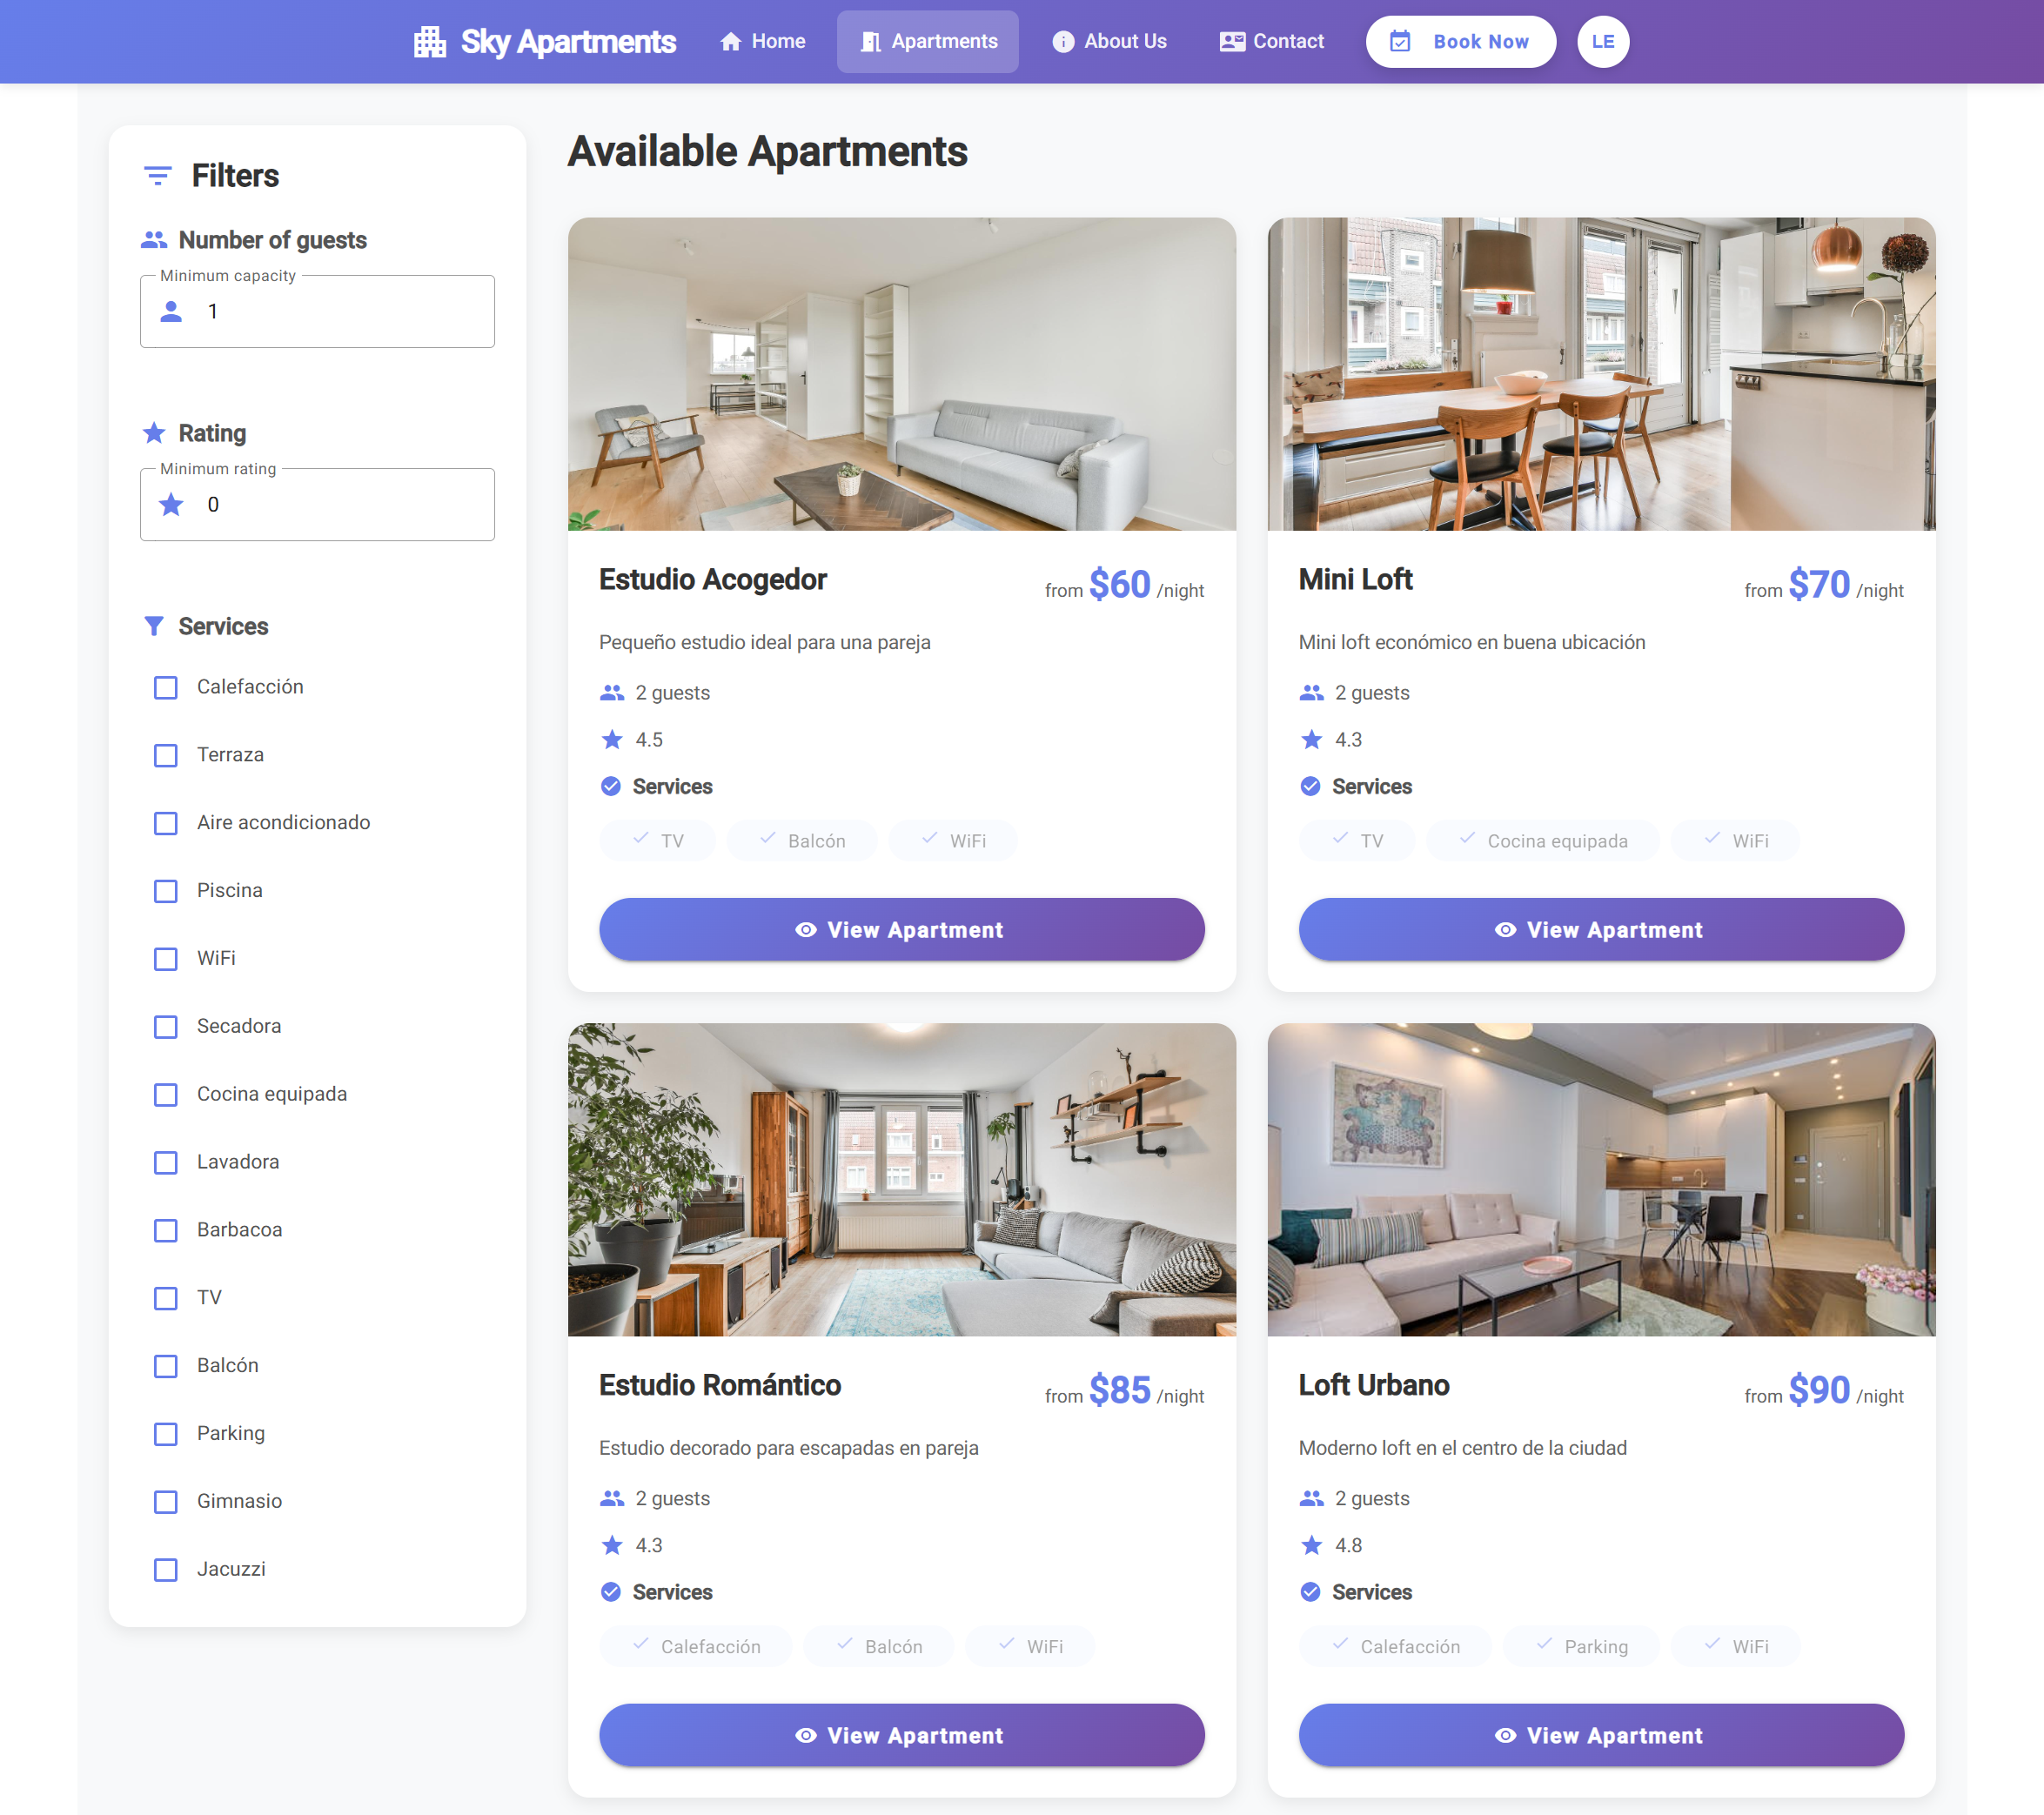
\includegraphics[width=0.8\textwidth]{img/advanced_filters_v1.png}
    \caption{Interfaz del motor de búsqueda con filtros avanzados combinados.}
    \label{fig:advanced_filters}
\end{figure}

\begin{figure}[!h]
    \centering
    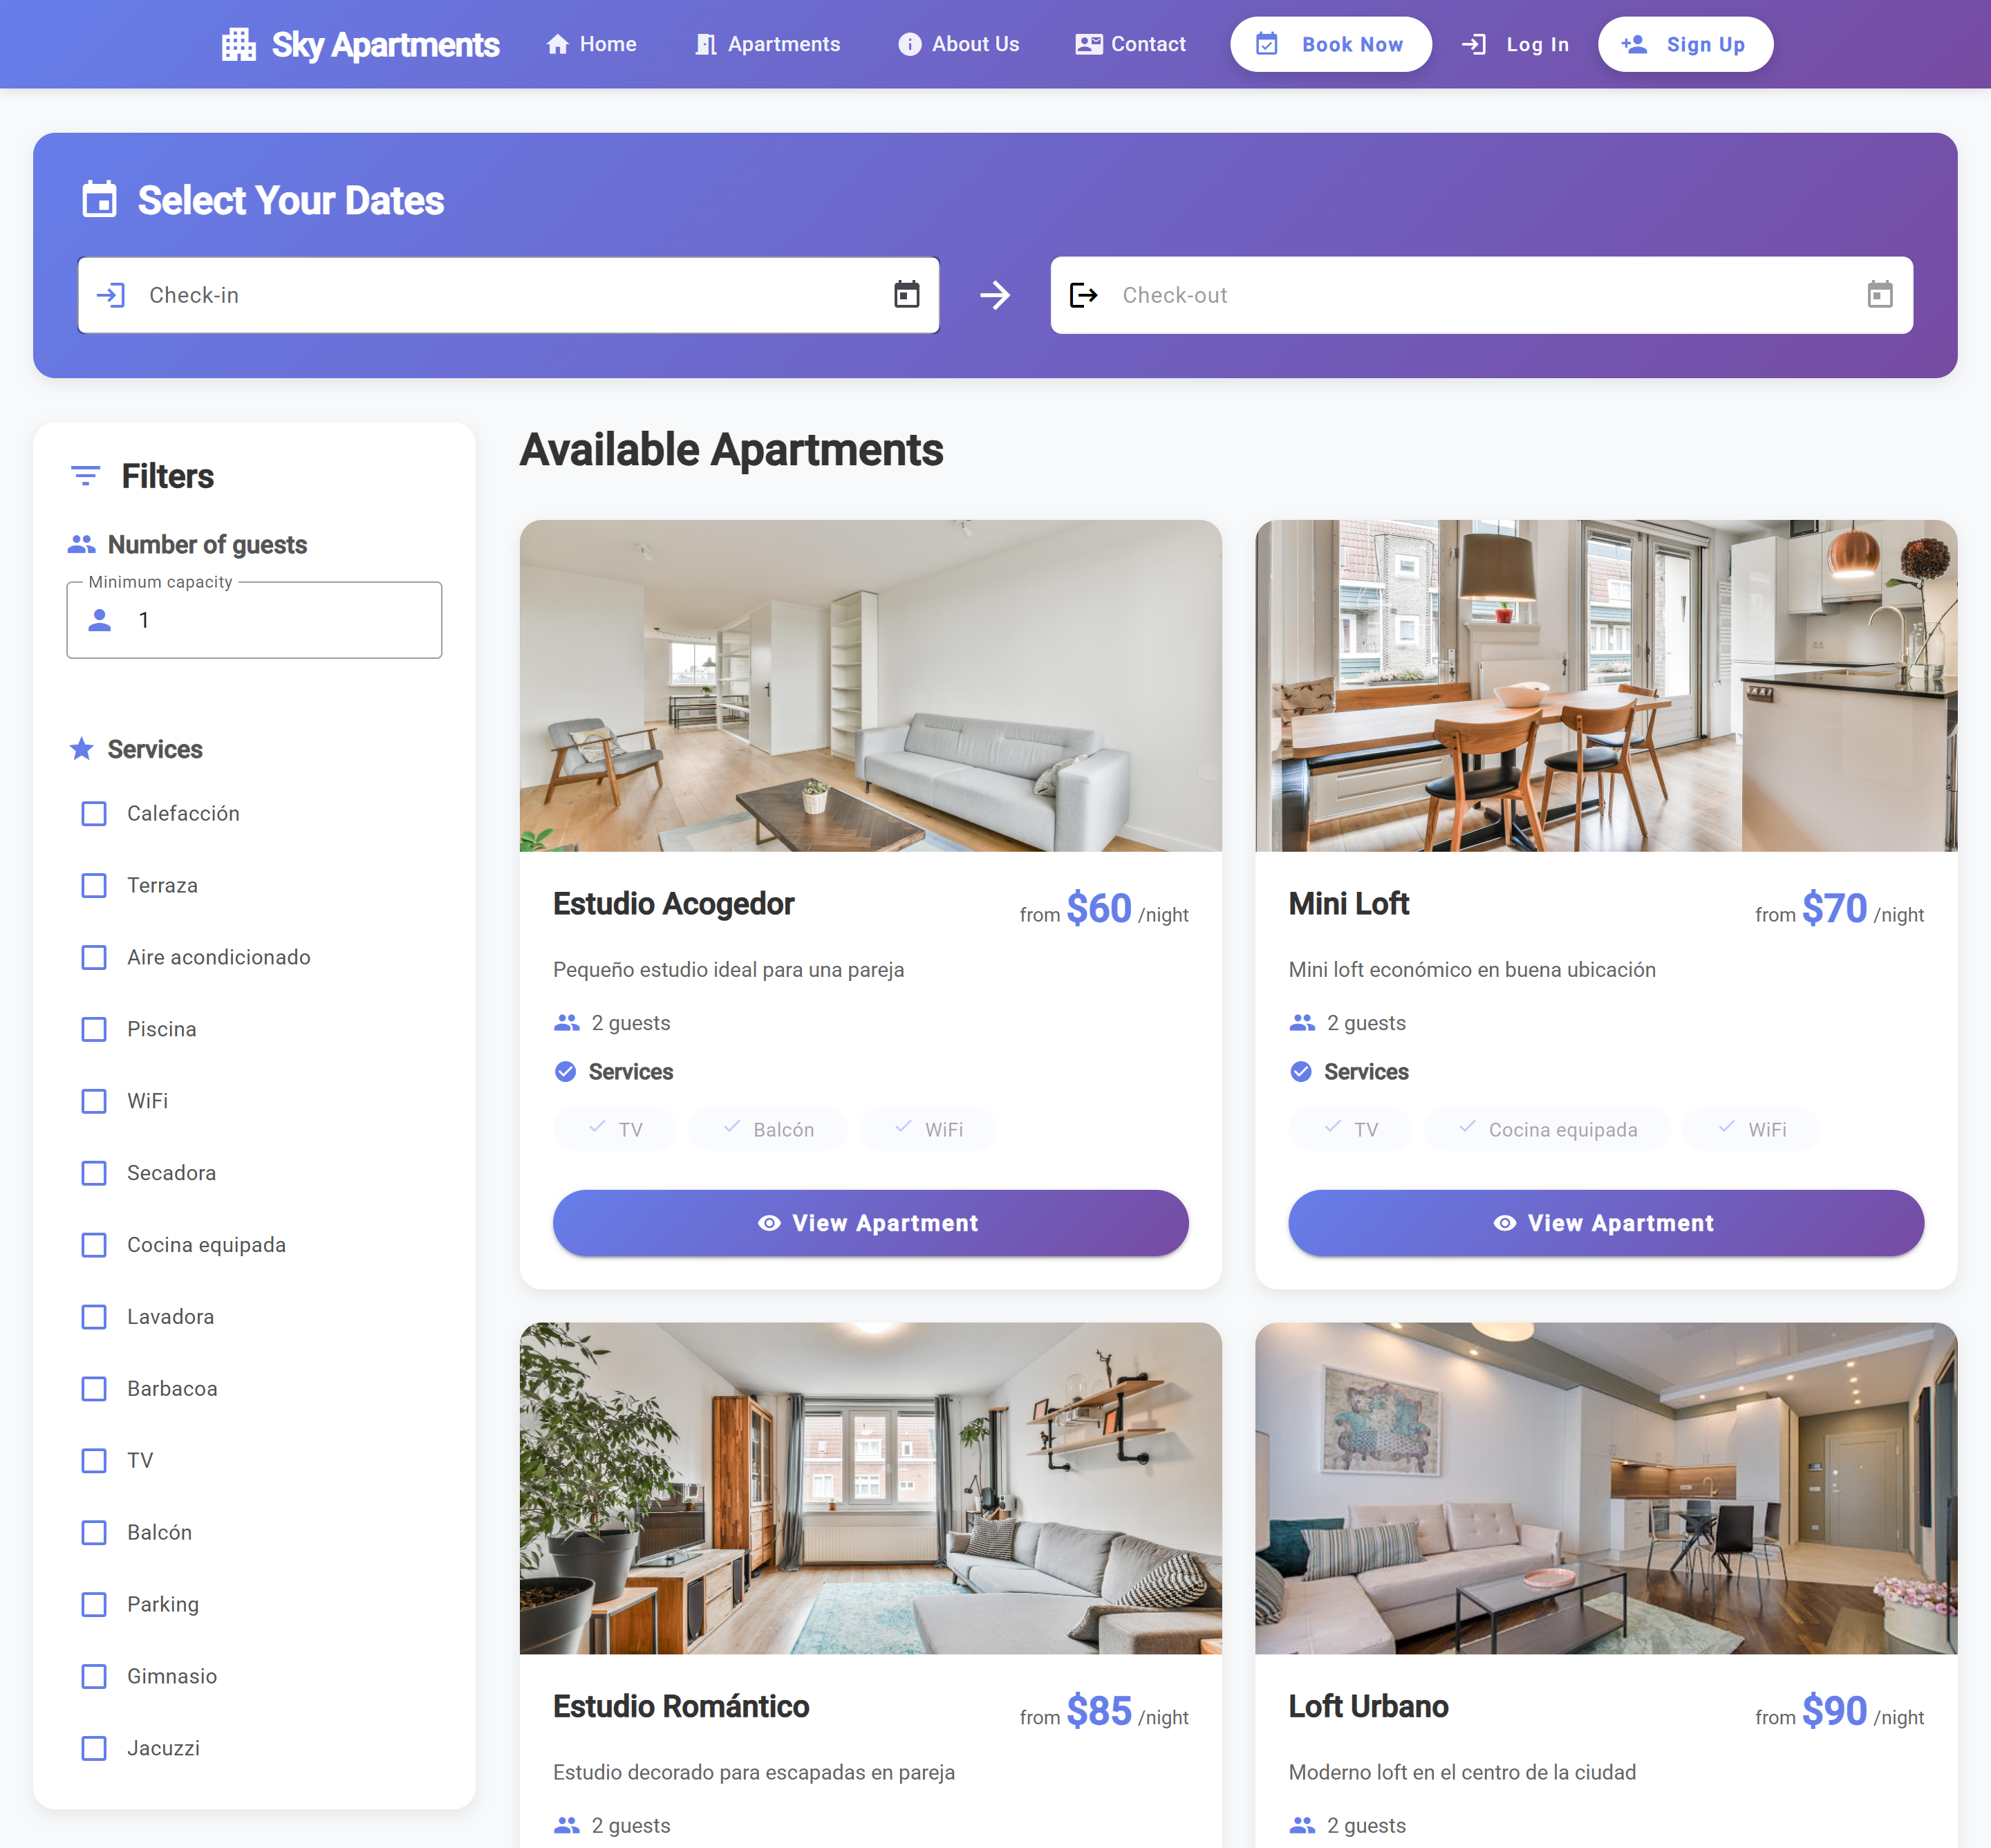
\includegraphics[width=0.8\textwidth]{img/catalogo_apartamentos_2.png}
    \caption{Interfaz del catálogo de apartamentos con filtro por fecha.}
    \label{fig:catalogo_apartamentos}
\end{figure}

\subsection{Detalles del Apartamento e Interfaz de Precios}
Cada alojamiento dispone de una página de detalle exhaustiva. En ella, el usuario puede interactuar con una galería multimedia de alta calidad,  consultar la descripción completa y los servicios incluidos (ver Figura \ref{fig:apartment_detail}).

Uno de los aspectos más destacados de esta vista es el \textbf{calendario interactivo con precios dinámicos}. El sistema no muestra una tarifa plana, sino que calcula y muestra variaciones de precio basadas en la temporada (alta, media, baja), el día de la semana (fines de semana), la proximidad de la fecha de reserva (\textit{last-minute}) o cualquier ajuste del precio que configure el administrador. Esto ofrece total transparencia al usuario, mostrando el desglose entre el precio base y las modificaciones aplicadas.

\begin{figure}[!h]
    \centering
    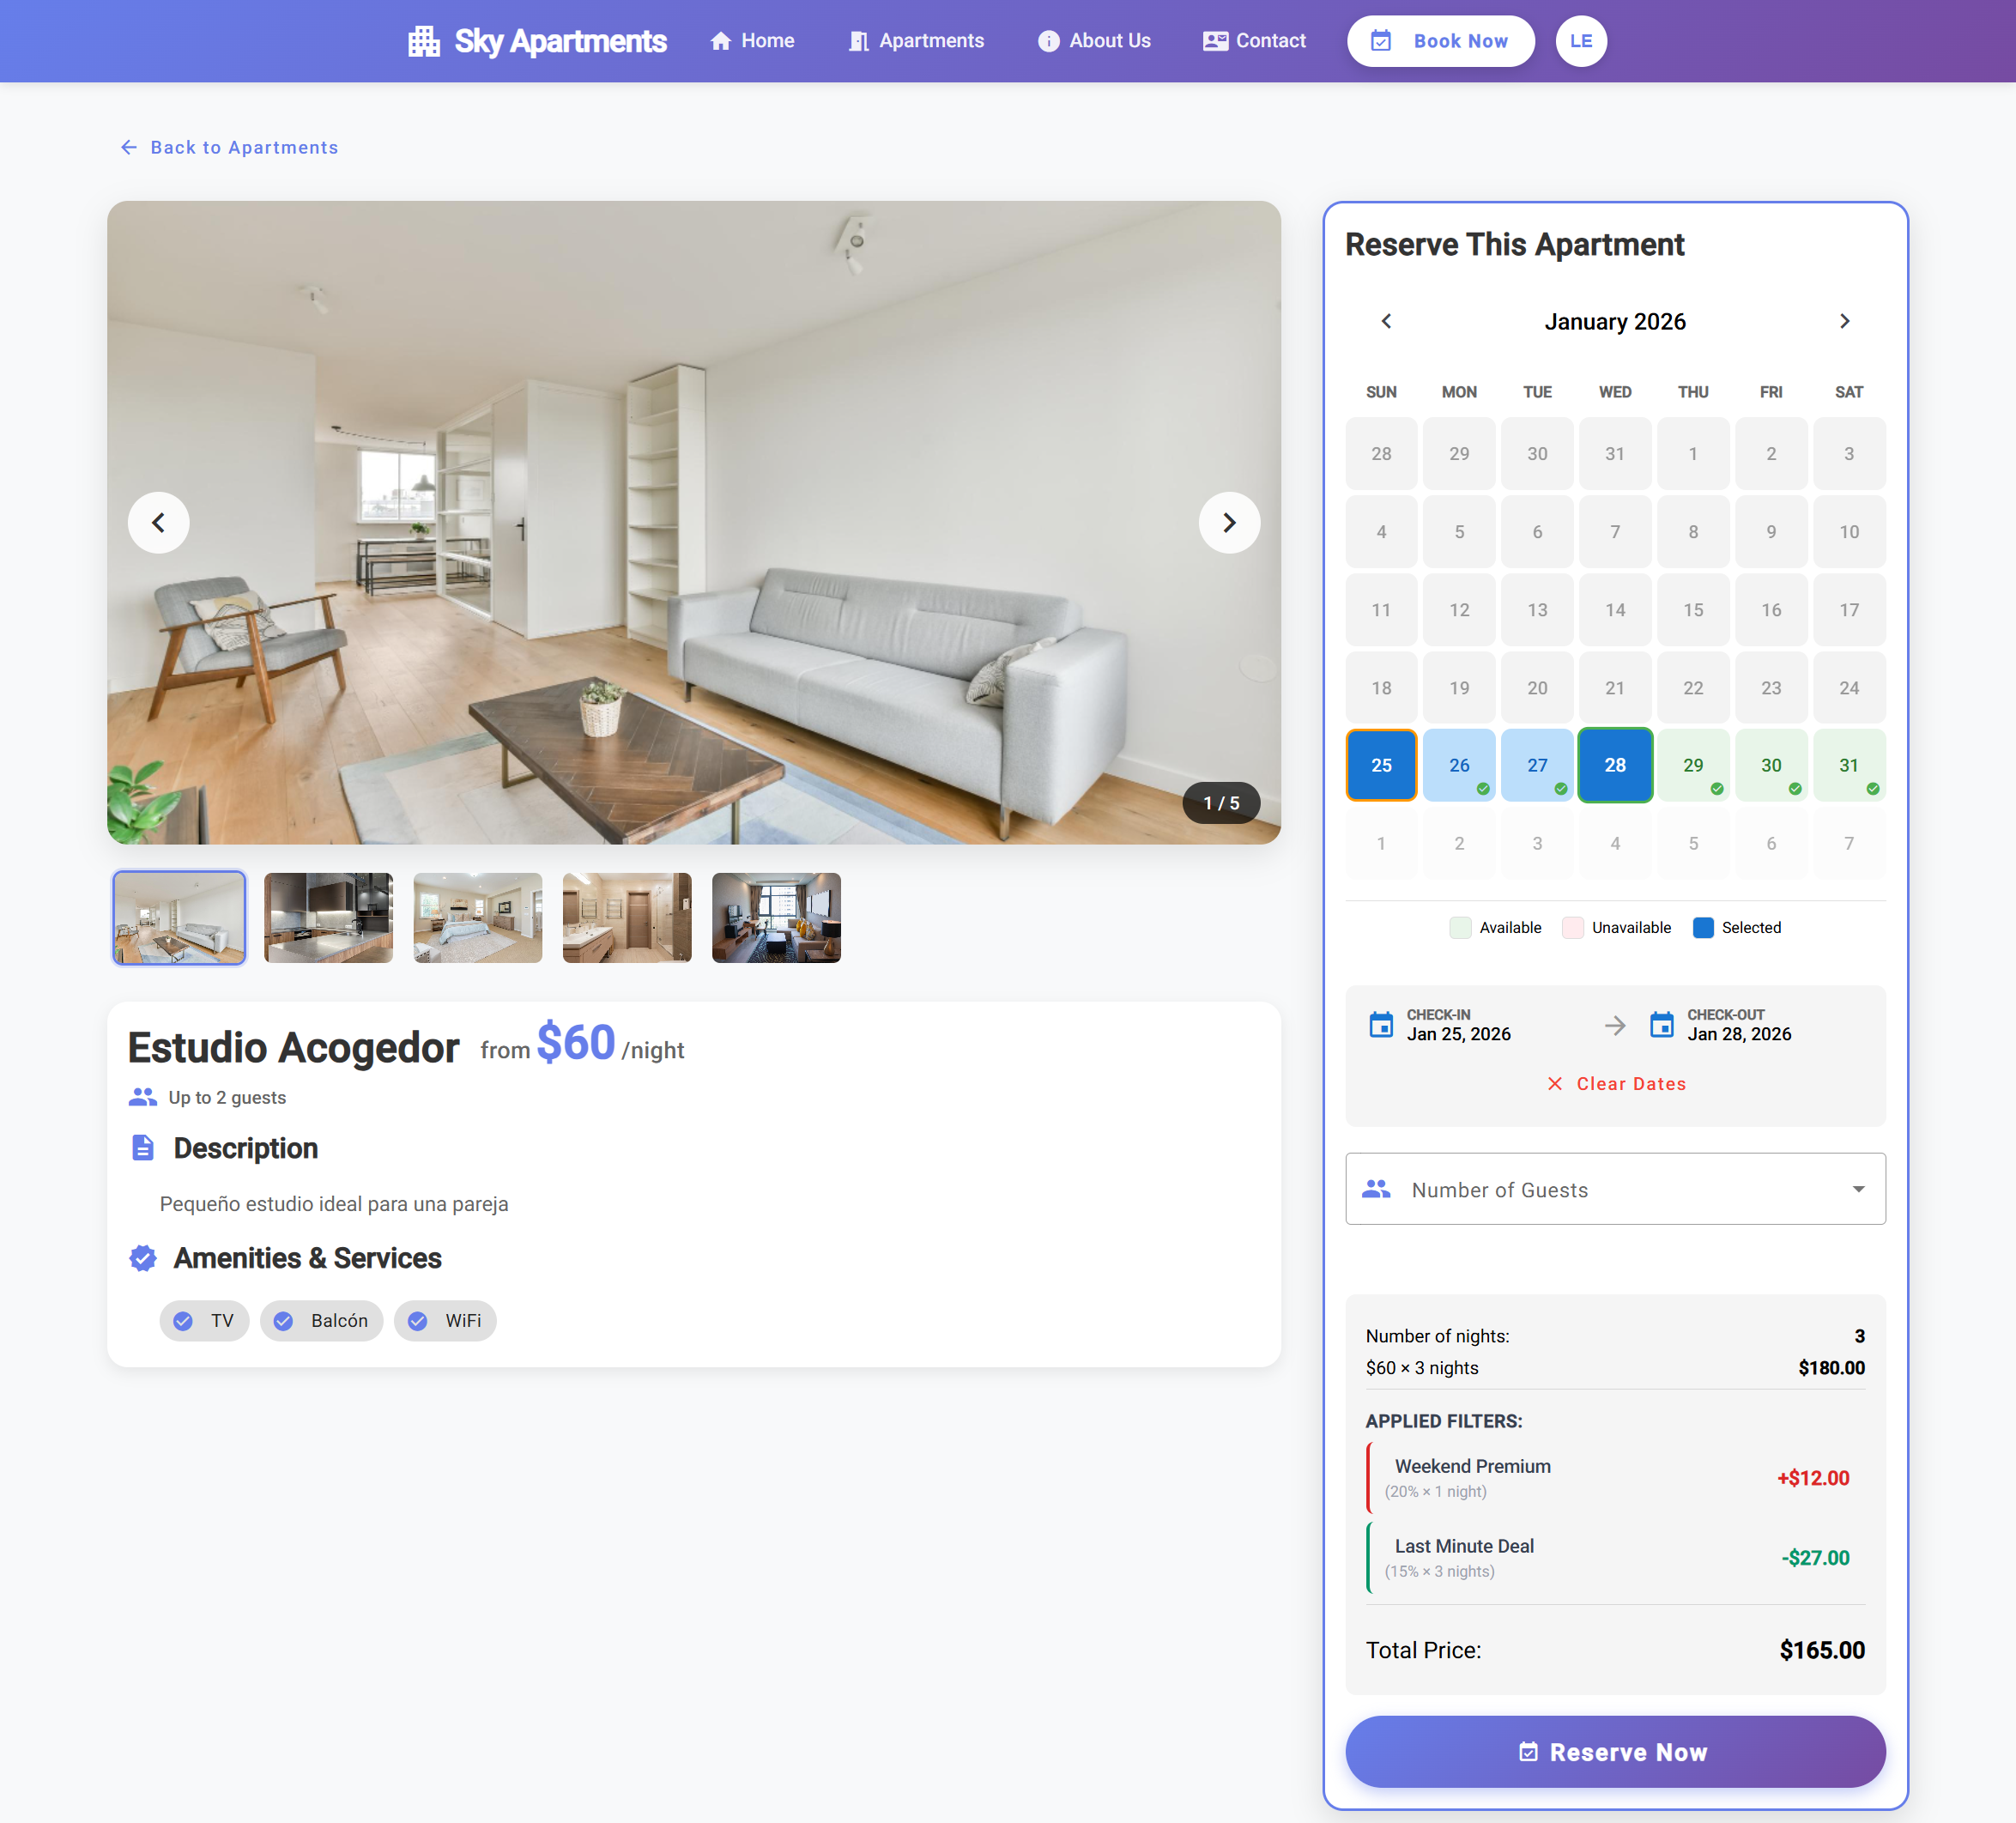
\includegraphics[width=1\textwidth]{img/apartment_detail_v1.png}
    \caption{Página de detalle del apartamento mostrando la galería multimedia y el calendario dinámico con precios.}
    \label{fig:apartment_detail}
\end{figure}

\section{Gestión del Ciclo de Vida de la Reserva}

El proceso de reserva ha sido diseñado para ser intuitivo y seguro. Una vez que el usuario registrado selecciona las fechas y el número de huéspedes, el sistema presenta un resumen detallado con el desglose final del precio.

\subsection{Sincronización y Notificaciones}
Al confirmar una reserva, el sistema ejecuta dos acciones críticas de forma simultánea:
\begin{enumerate}
    \item \textbf{Sincronización inmediata:} Actualiza el calendario global de disponibilidad en tiempo real, bloqueando las fechas para evitar cualquier posibilidad de \textit{overbooking}.
    \item \textbf{Notificaciones transaccionales automáticas:} El usuario recibe correos electrónicos automáticos en cada etapa de la reserva: confirmaciones, actualizaciones, cancelaciones y recordatorios de \textit{check-in} (ver Figura~\ref{fig:booking_confirmation}).
\end{enumerate}

\begin{figure}[!h]
    \centering
    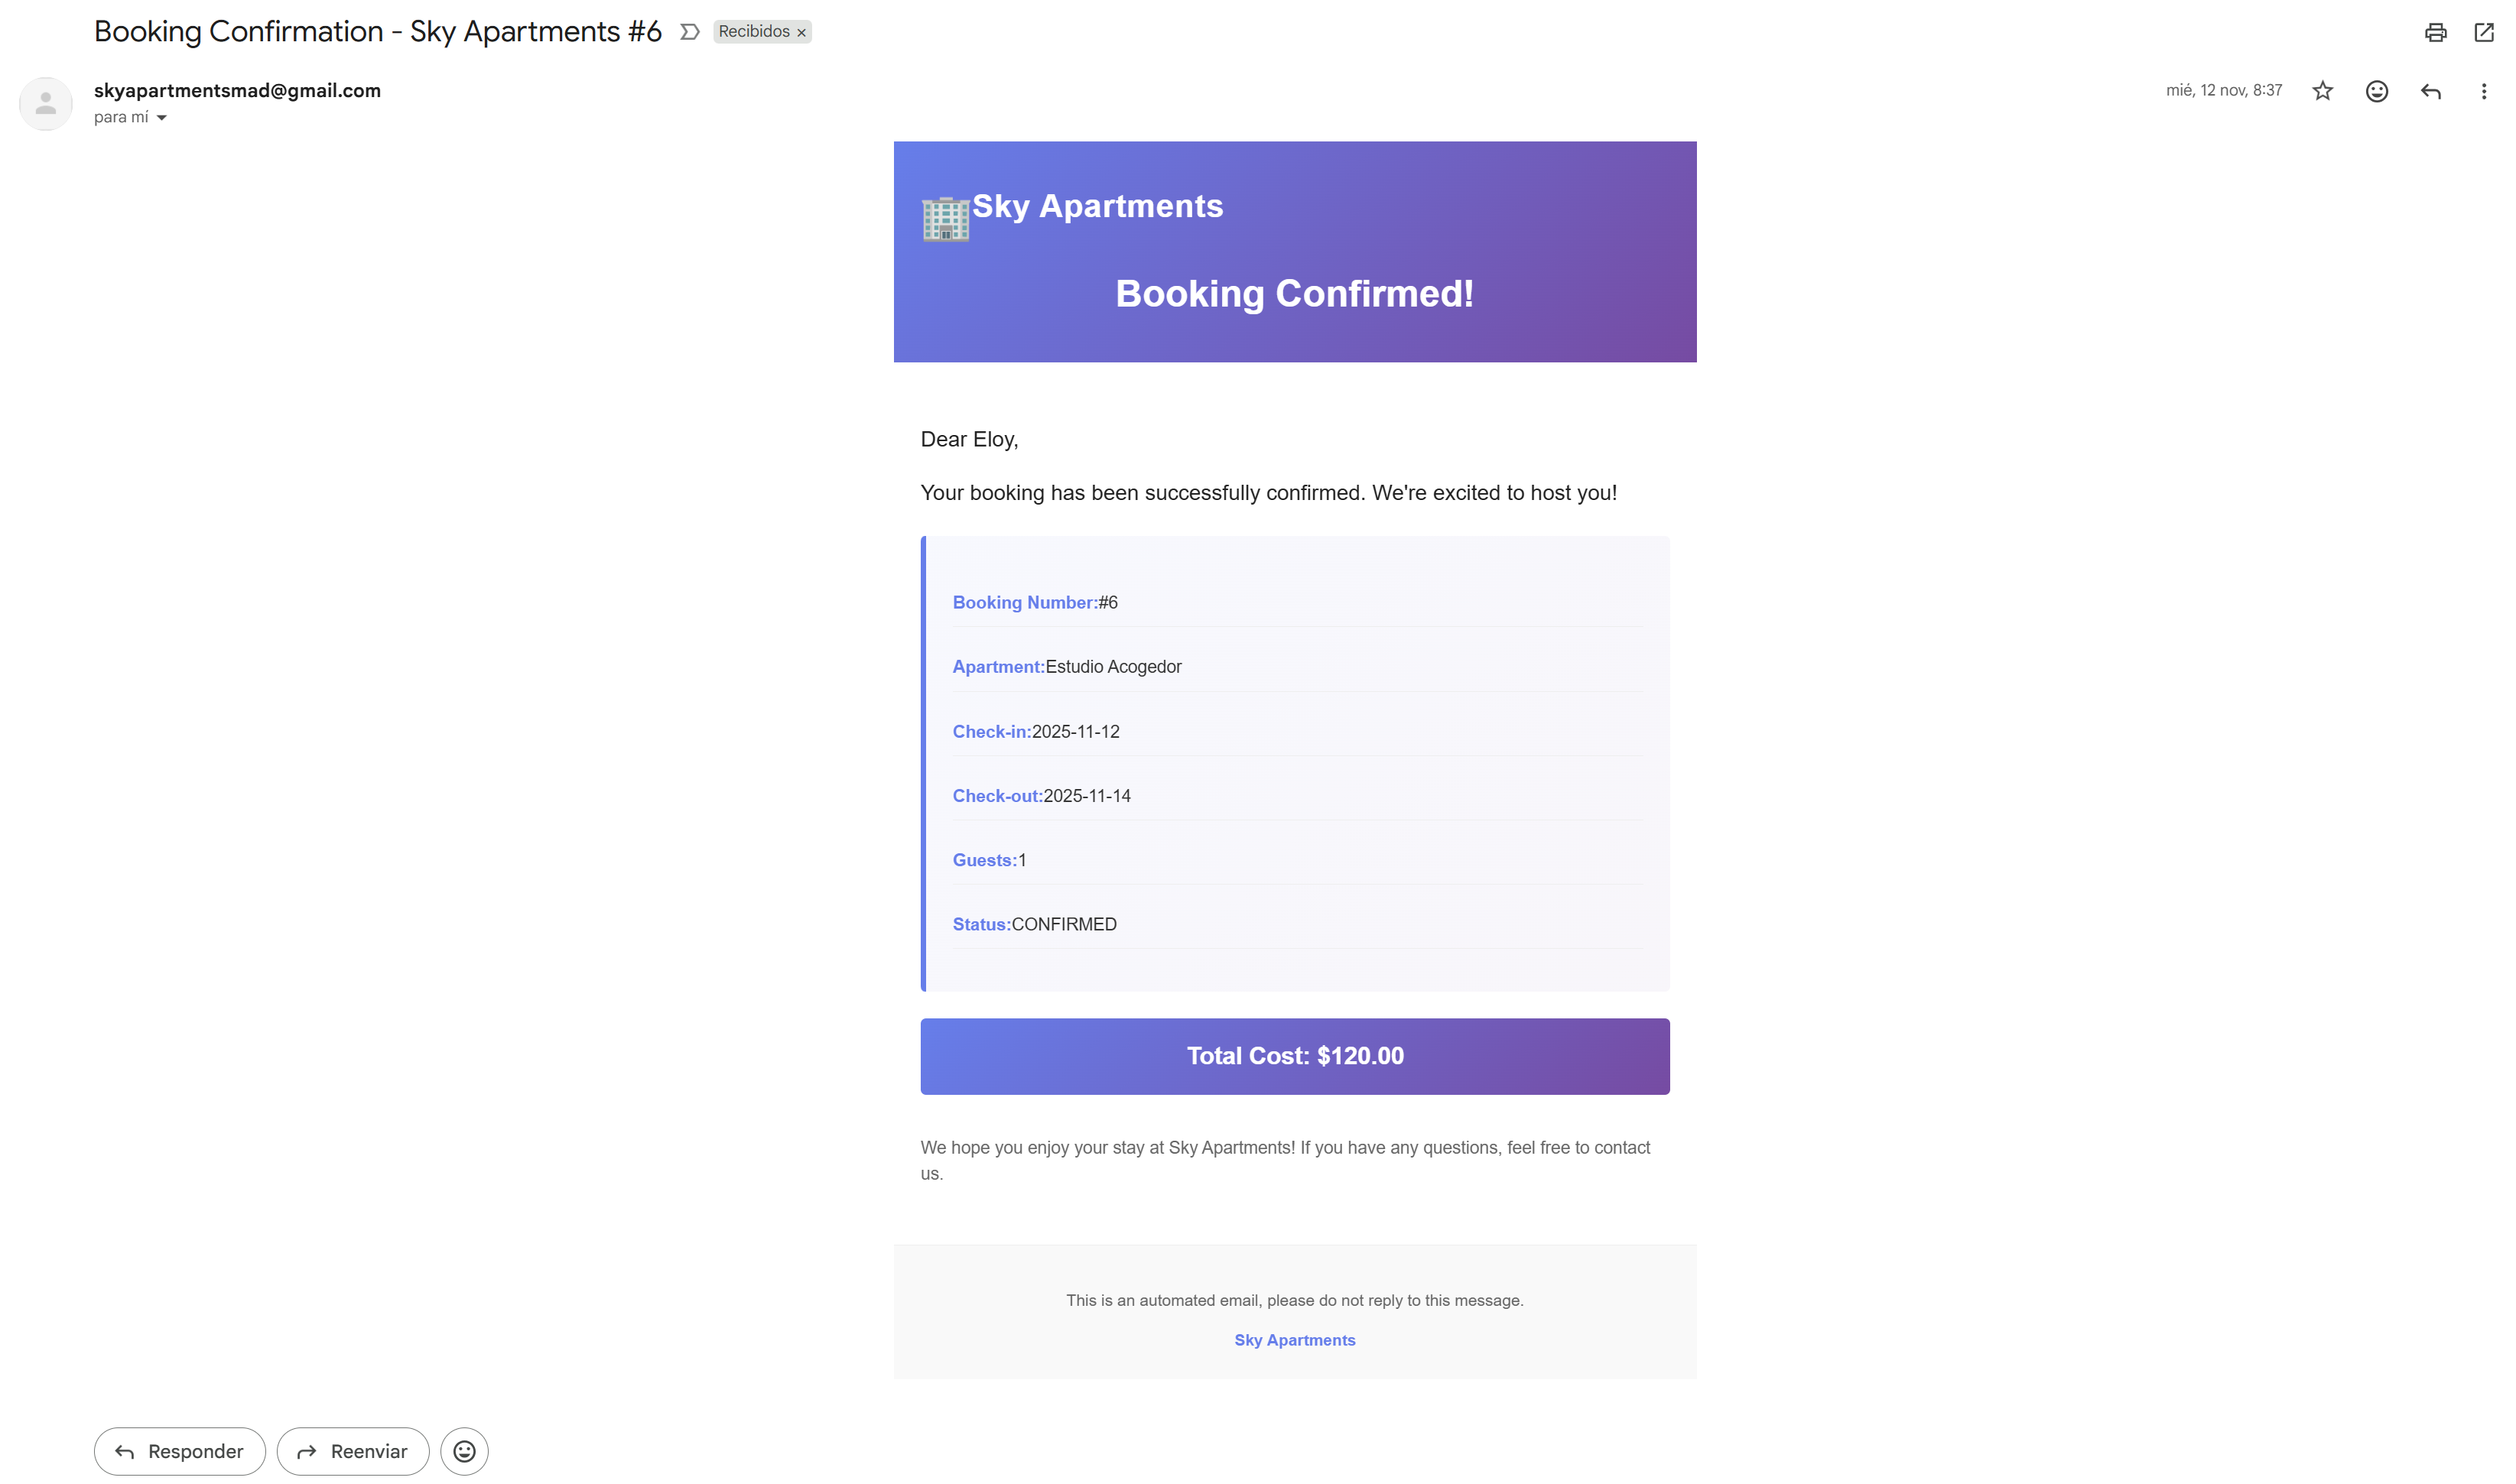
\includegraphics[width=1\textwidth]{img/booking_confirmation_v02.png}
    \caption{Ejemplo de notificación de confirmación de reserva enviada al usuario.}
    \label{fig:booking_confirmation}
\end{figure}

\section{Área de Usuario y Sistema de Reseñas}
Esta sección describe el panel personal del usuario registrado, desde el que puede gestionar su perfil e historial de estancias, y el sistema de reseñas para valorar los alojamientos tras su visita.
\subsection{Perfil e Historial}
Los usuarios registrados disponen de un panel personal donde pueden actualizar sus datos y consultar su historial completo de reservas. Este panel categoriza las reservas por estado (confirmadas, canceladas o completadas) y permite la cancelación ágil de estancias futuras.

\subsection{Valoraciones y Prueba Social}
Para fomentar la confianza en la plataforma, se ha implementado un sistema de reseñas. Una vez que el estado de una reserva pasa a "completada" (tras el \textit{check-out}), el usuario queda habilitado para puntuar el alojamiento (1-5 estrellas) y redactar un comentario detallado sobre su experiencia. Estas reseñas se publican en la página del apartamento, alimentando el algoritmo de valoración media (ver Figura \ref{fig:reviews}).

\begin{figure}[!h]
    \centering
    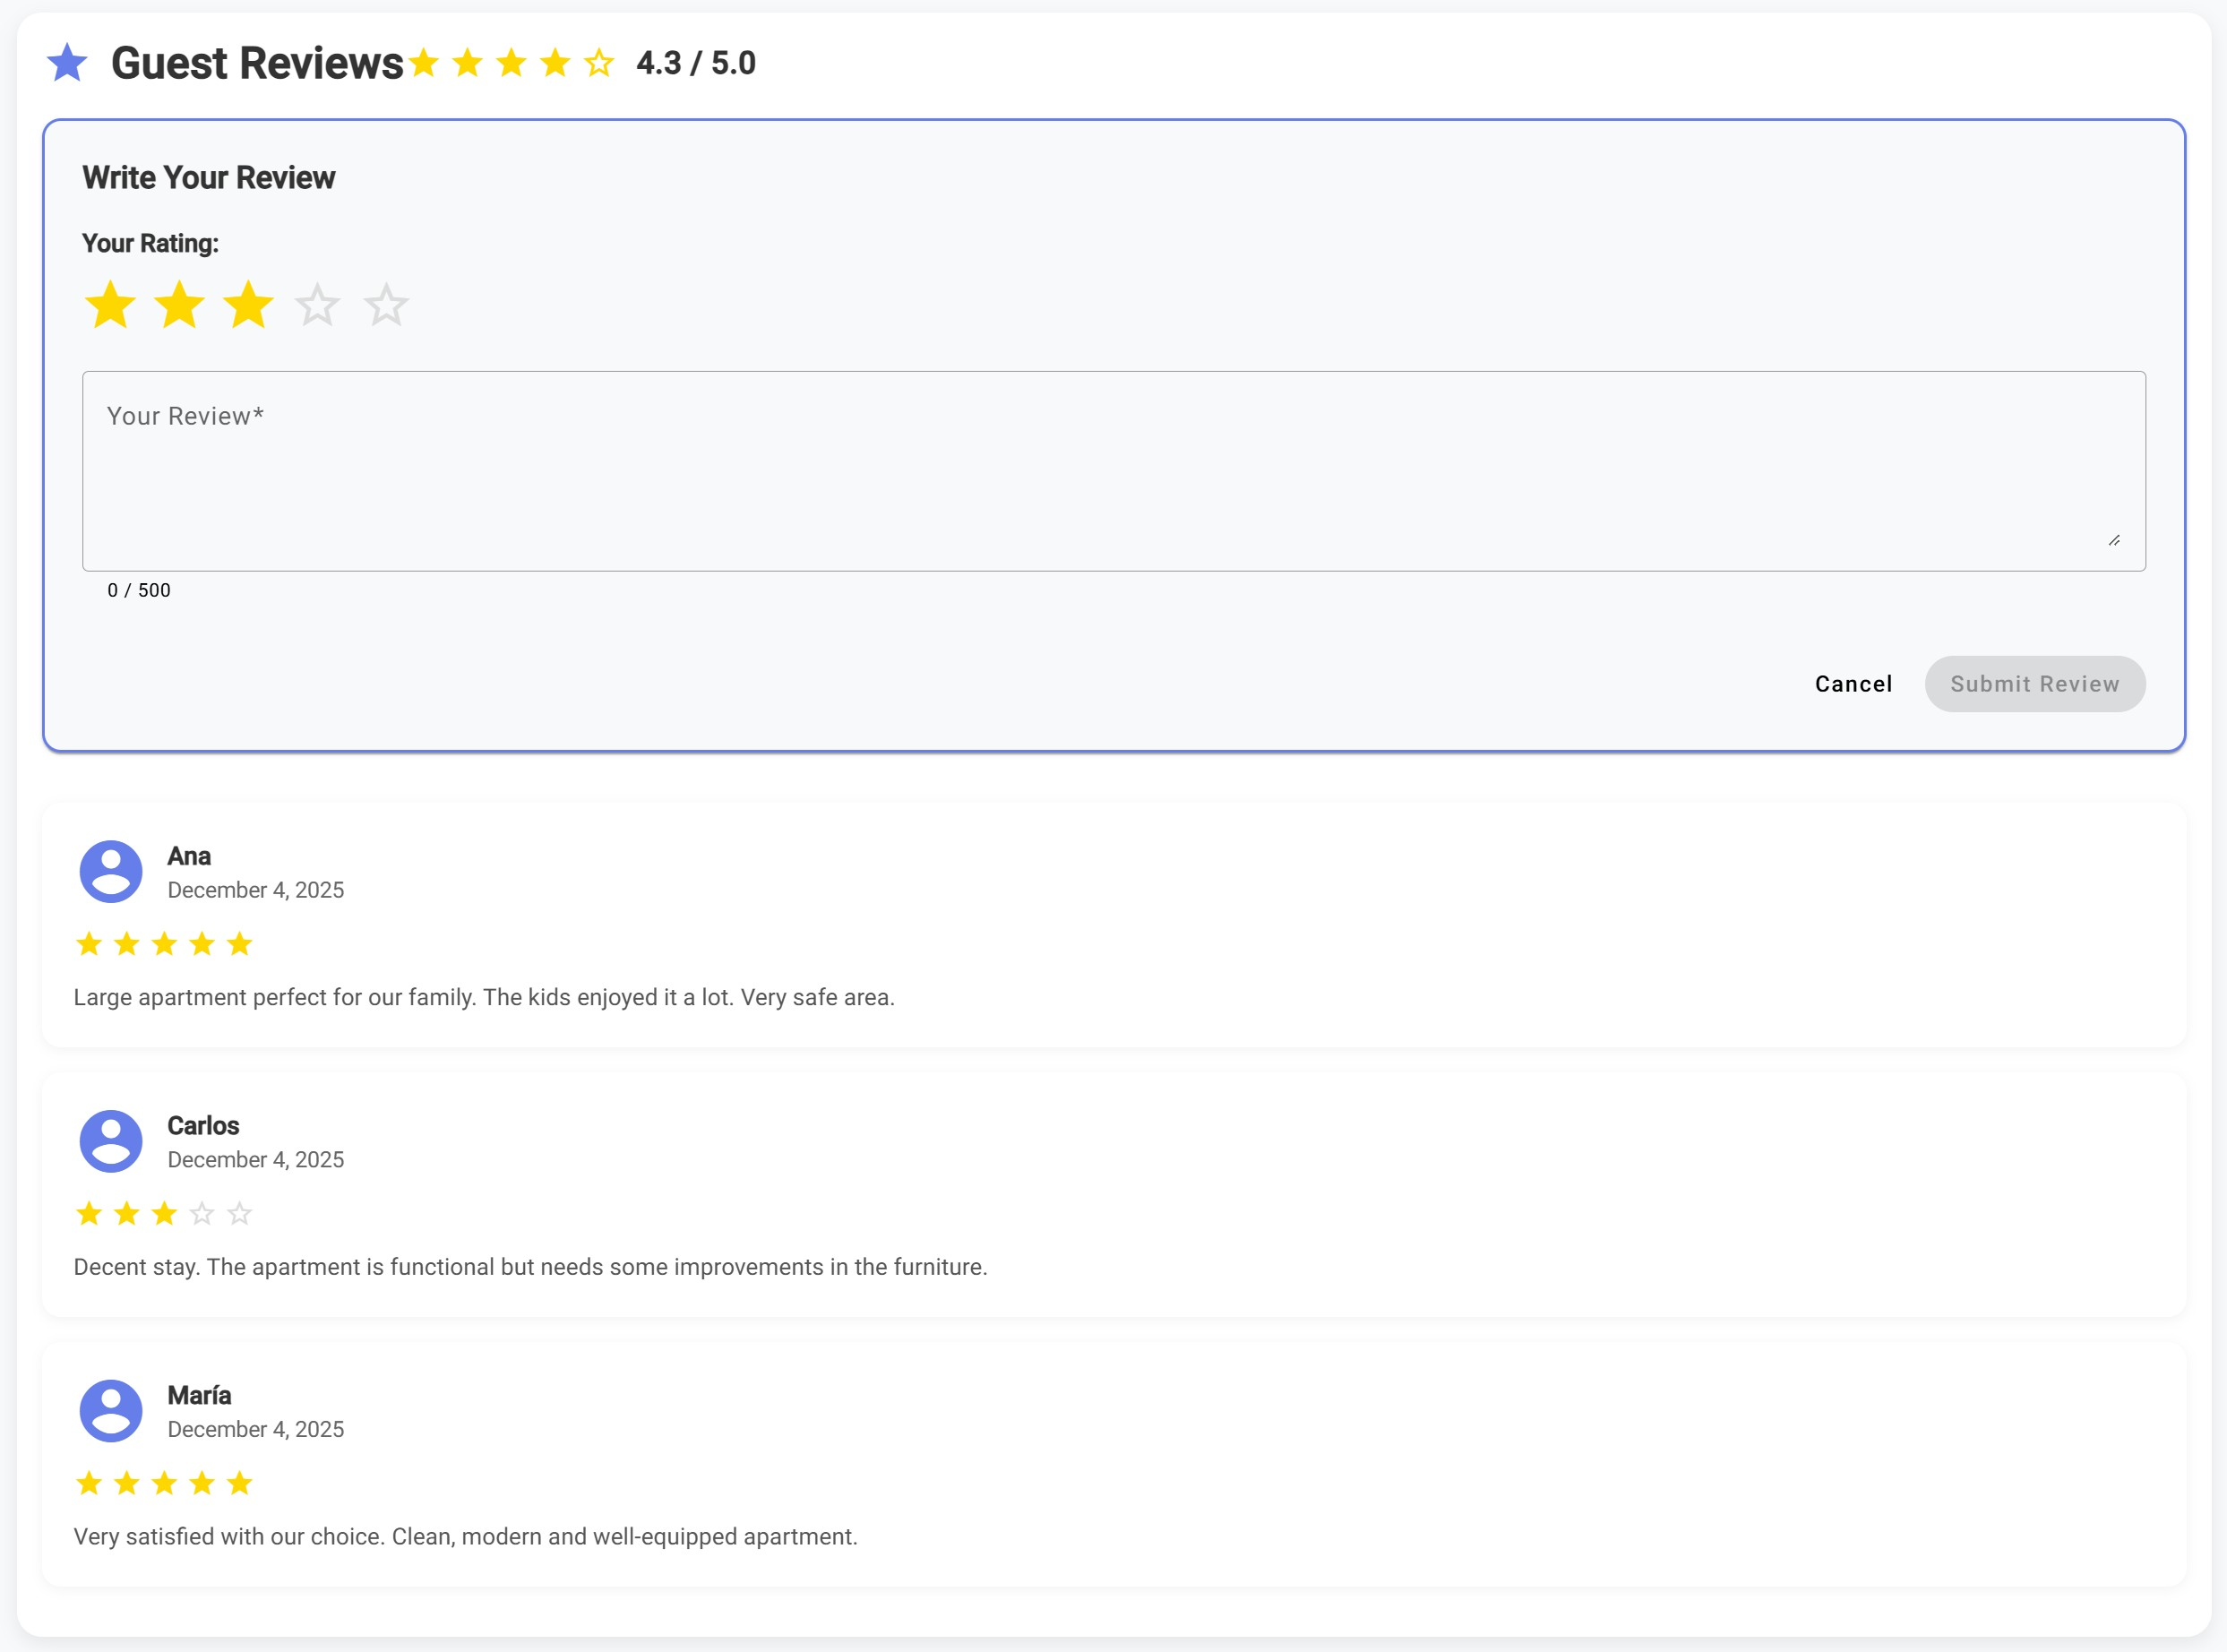
\includegraphics[width=0.9\textwidth]{img/reviews_v02.jpg}
    \caption{Sistema de valoraciones y reseñas integrado en la plataforma.}
    \label{fig:reviews}
\end{figure}

\section{Panel de Administración (Dashboard)}

El panel de administración dota al propietario de un control absoluto sobre su negocio a través de cuatro módulos principales.

\subsection{Analítica y Estadísticas}
El sistema genera representaciones visuales e indicadores clave de rendimiento (\textit{Key Performance Indicators}, KPIs) 
en tiempo real para el período seleccionado, incluyendo ingresos totales, número de 
reservas activas, tasas de ocupación media, duración promedio de las estancias, rankings 
de alojamientos más demandados y mejor valorados, y un gráfico de evolución temporal de 
ocupación (ver Figura~\ref{fig:admin_dashboard}).

\begin{figure}[!h]
    \centering
    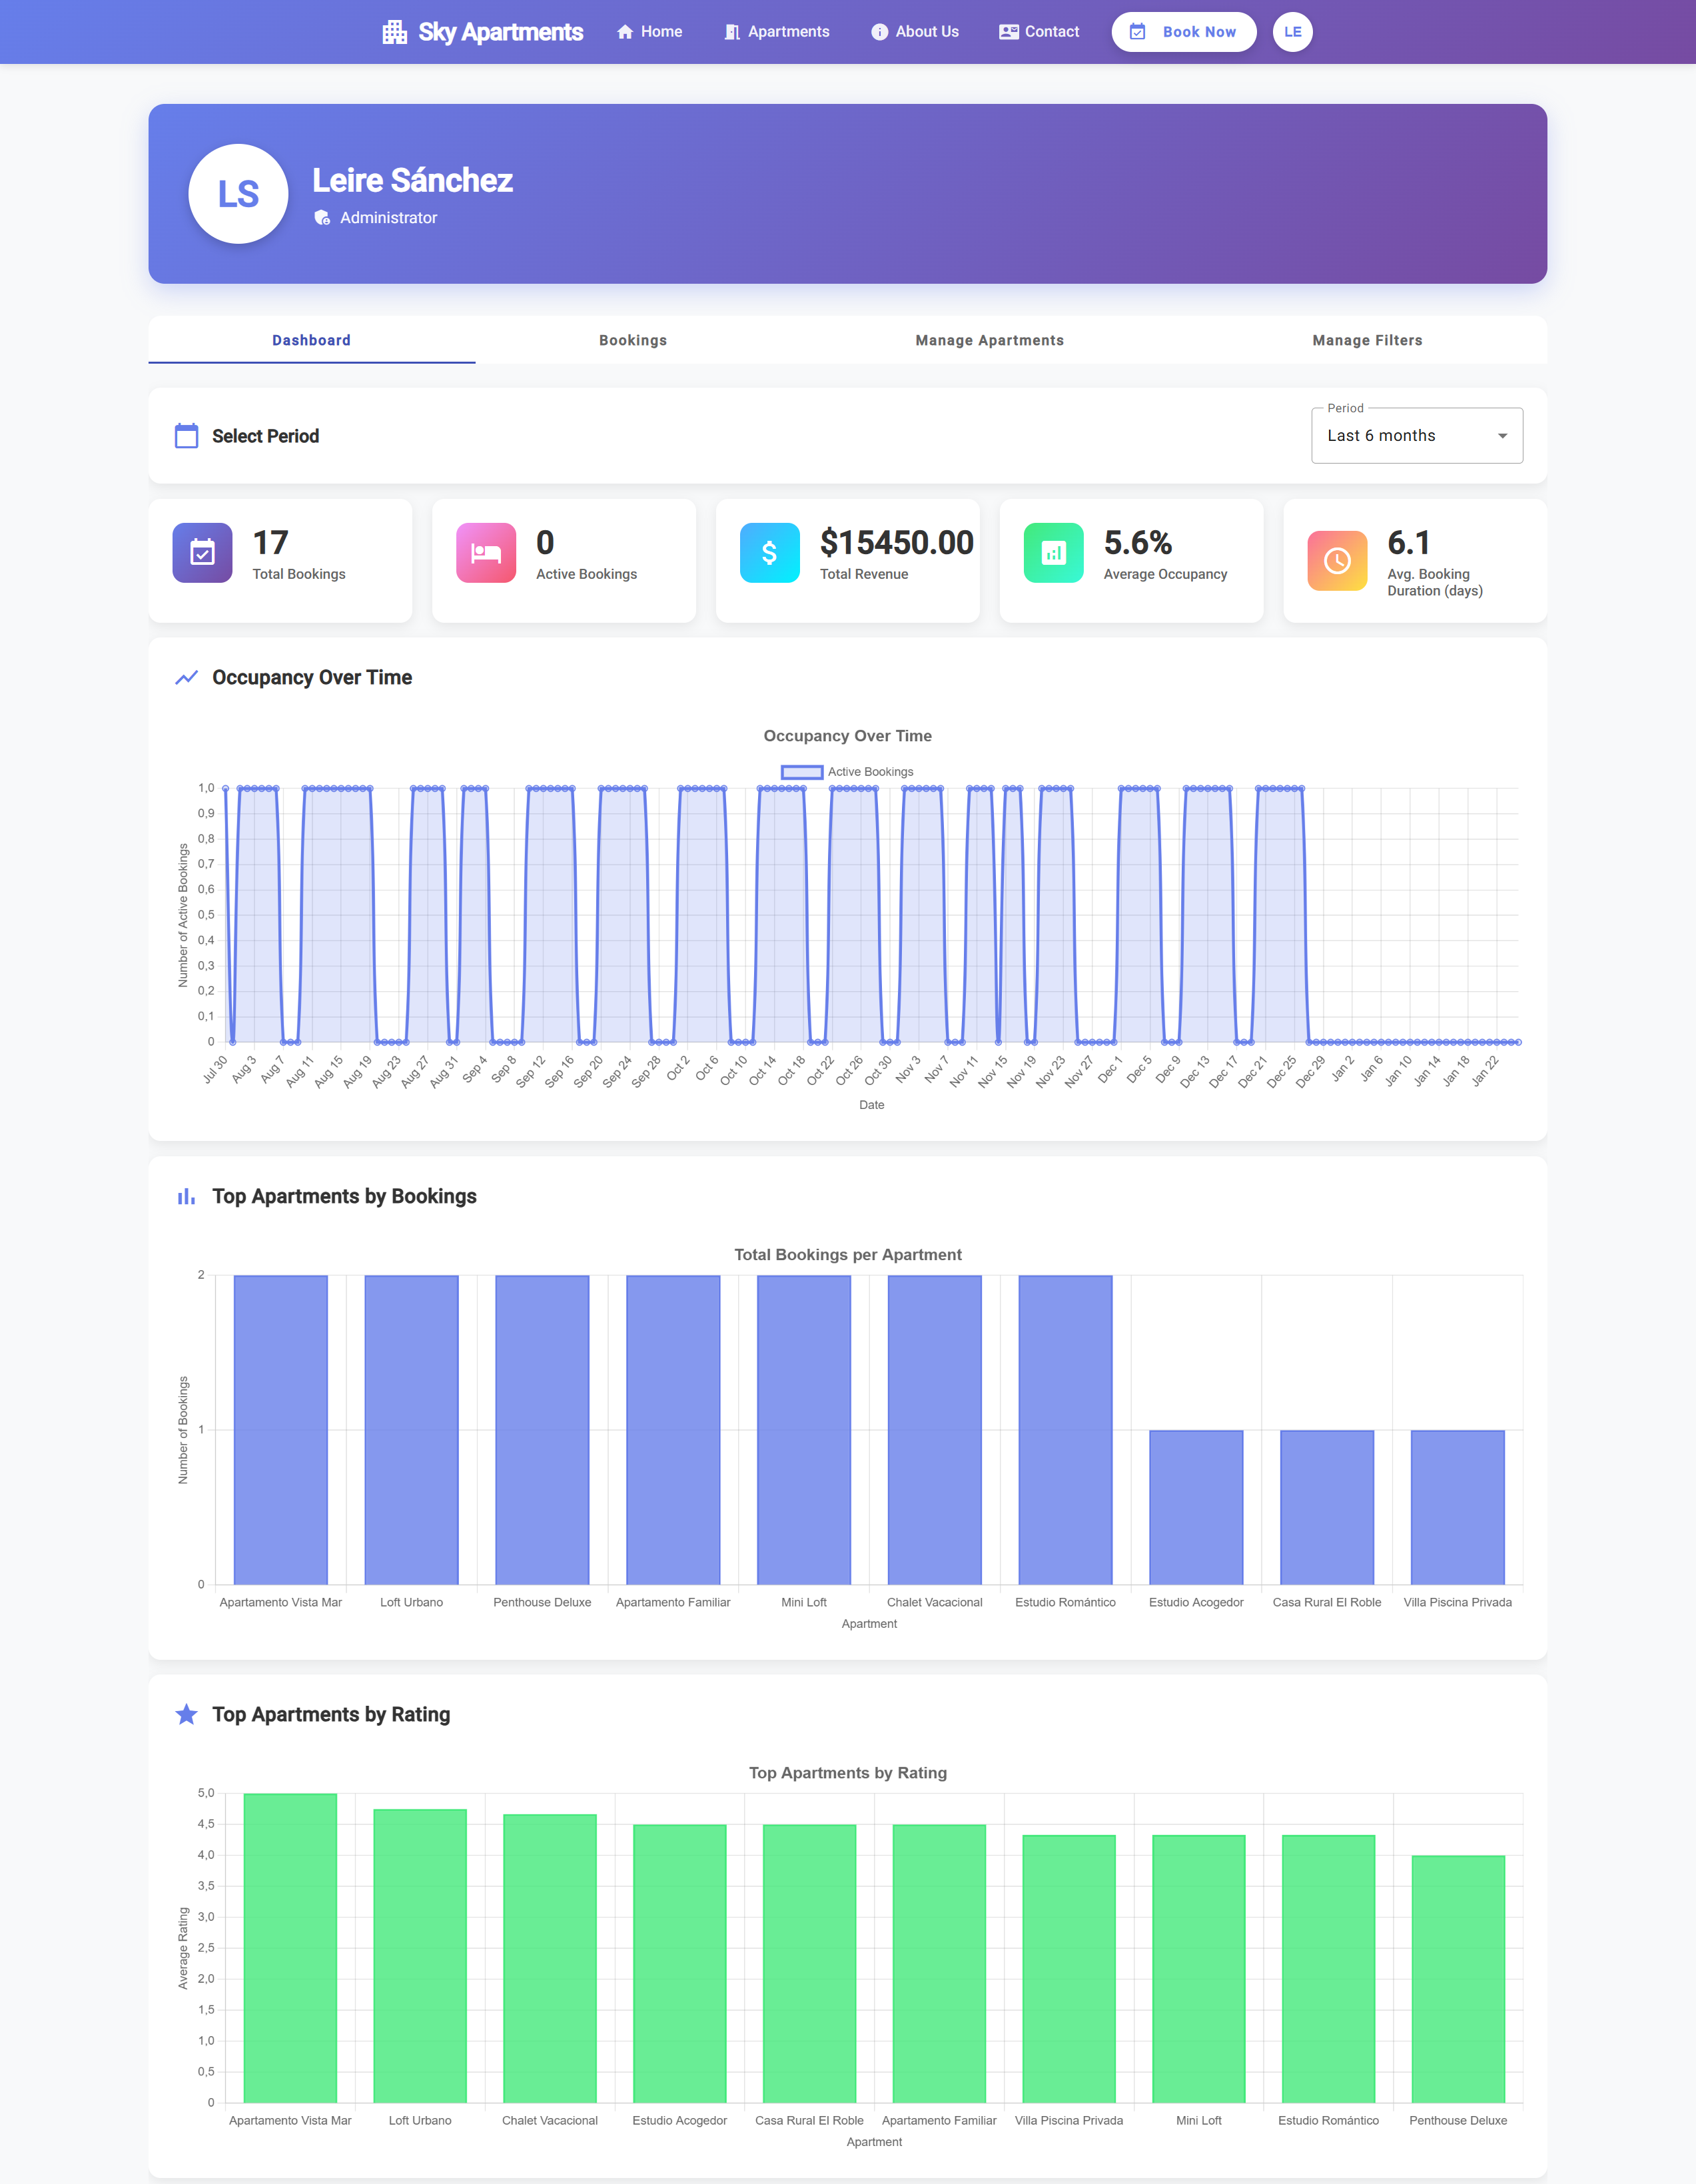
\includegraphics[width=0.9\textwidth]{img/admin_panel_v1.png}
    \caption{Dashboard analítico del panel de administración.}
    \label{fig:admin_dashboard}
\end{figure}

\subsection{Gestión de Apartamentos (CRUD)}
Desde este módulo, el administrador puede dar de alta, editar y eliminar apartamentos, gestionar sus galerías de imágenes y configurar sus características técnicas (capacidad, servicios incluidos, precio base) (ver Figura~\ref{fig:admin_apartments}).
\begin{figure}[!h]
    \centering
    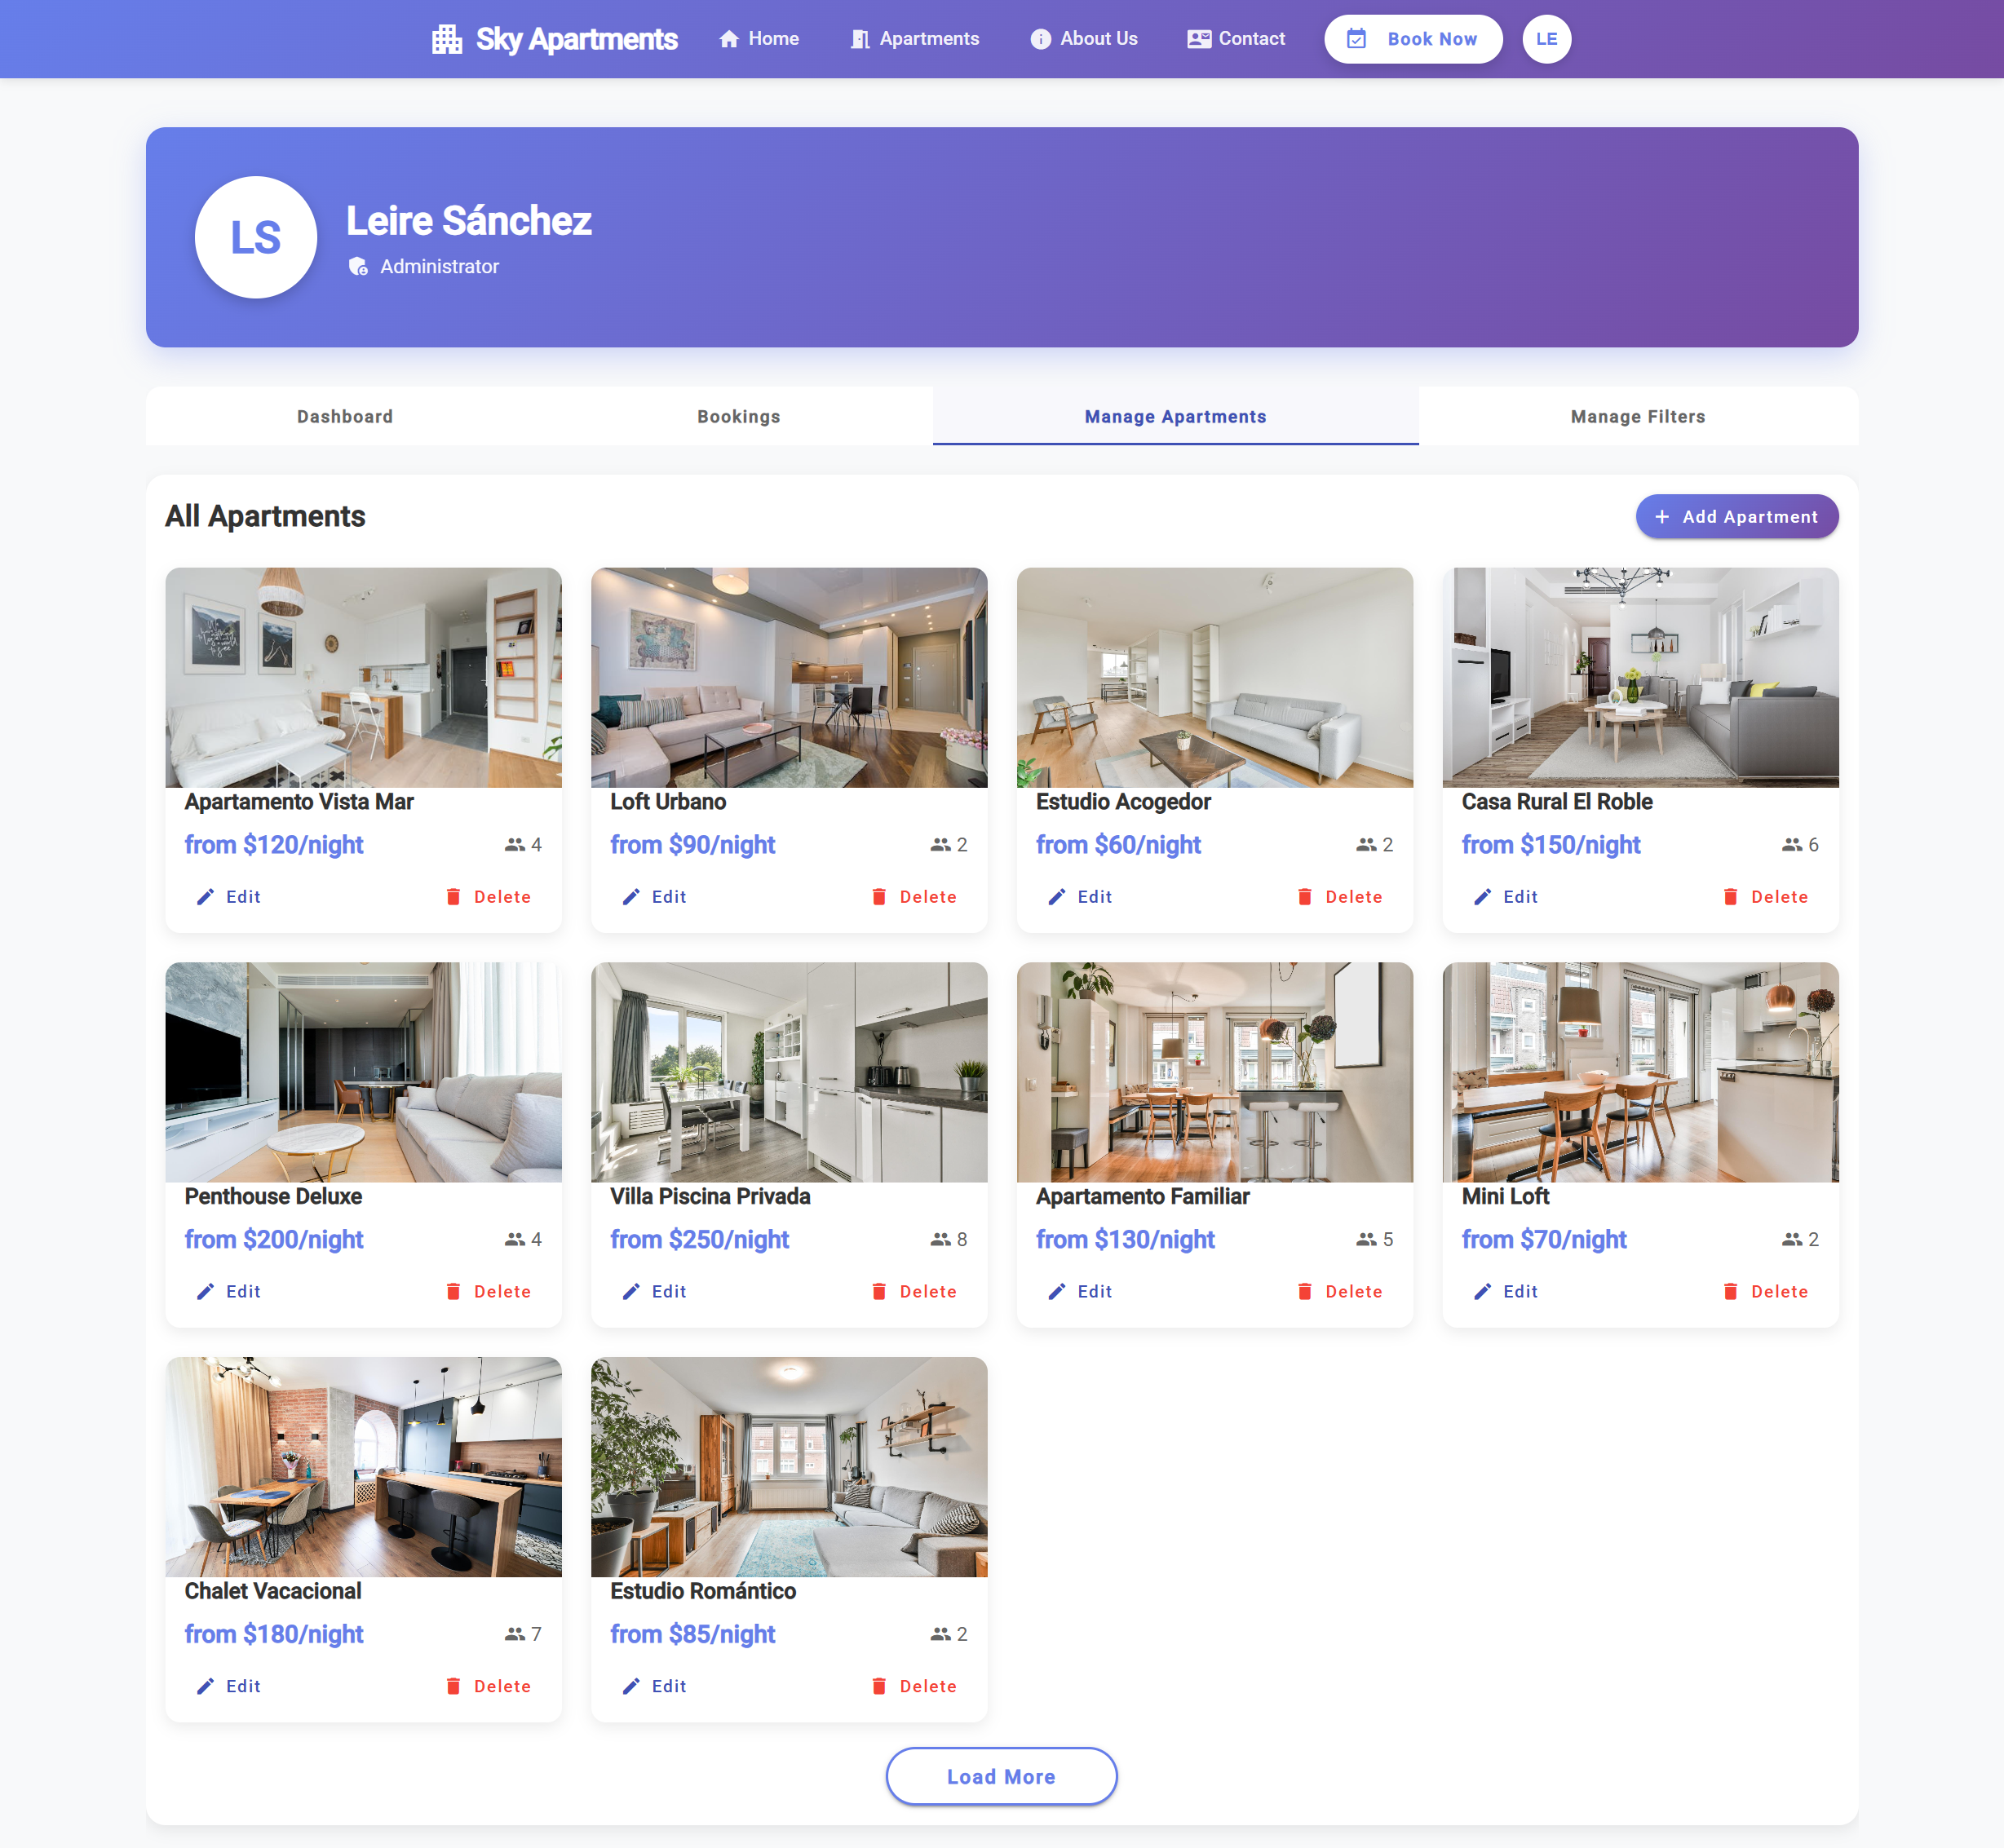
\includegraphics[width=0.9\textwidth]{img/admin_apartments_v1.png}
    \caption{Interfaz de gestión y edición del catálogo de apartamentos.}
    \label{fig:admin_apartments}
\end{figure}

\subsection{Gestión de Precios Dinámicos}
A nivel de negocio, este módulo independiente permite al administrador configurar las reglas del motor de precios dinámicos de forma visual. Desde aquí se pueden crear, activar o desactivar filtros de precio complejos: estableciendo multiplicadores de fin de semana, definiendo las fechas exactas de las distintas temporadas (alta, baja) y configurando ajustes automáticos por reservas de última hora (\textit{last minute}) o largas estancias (ver Figura \ref{fig:admin_filters}).

\begin{figure}[!h]
    \centering
    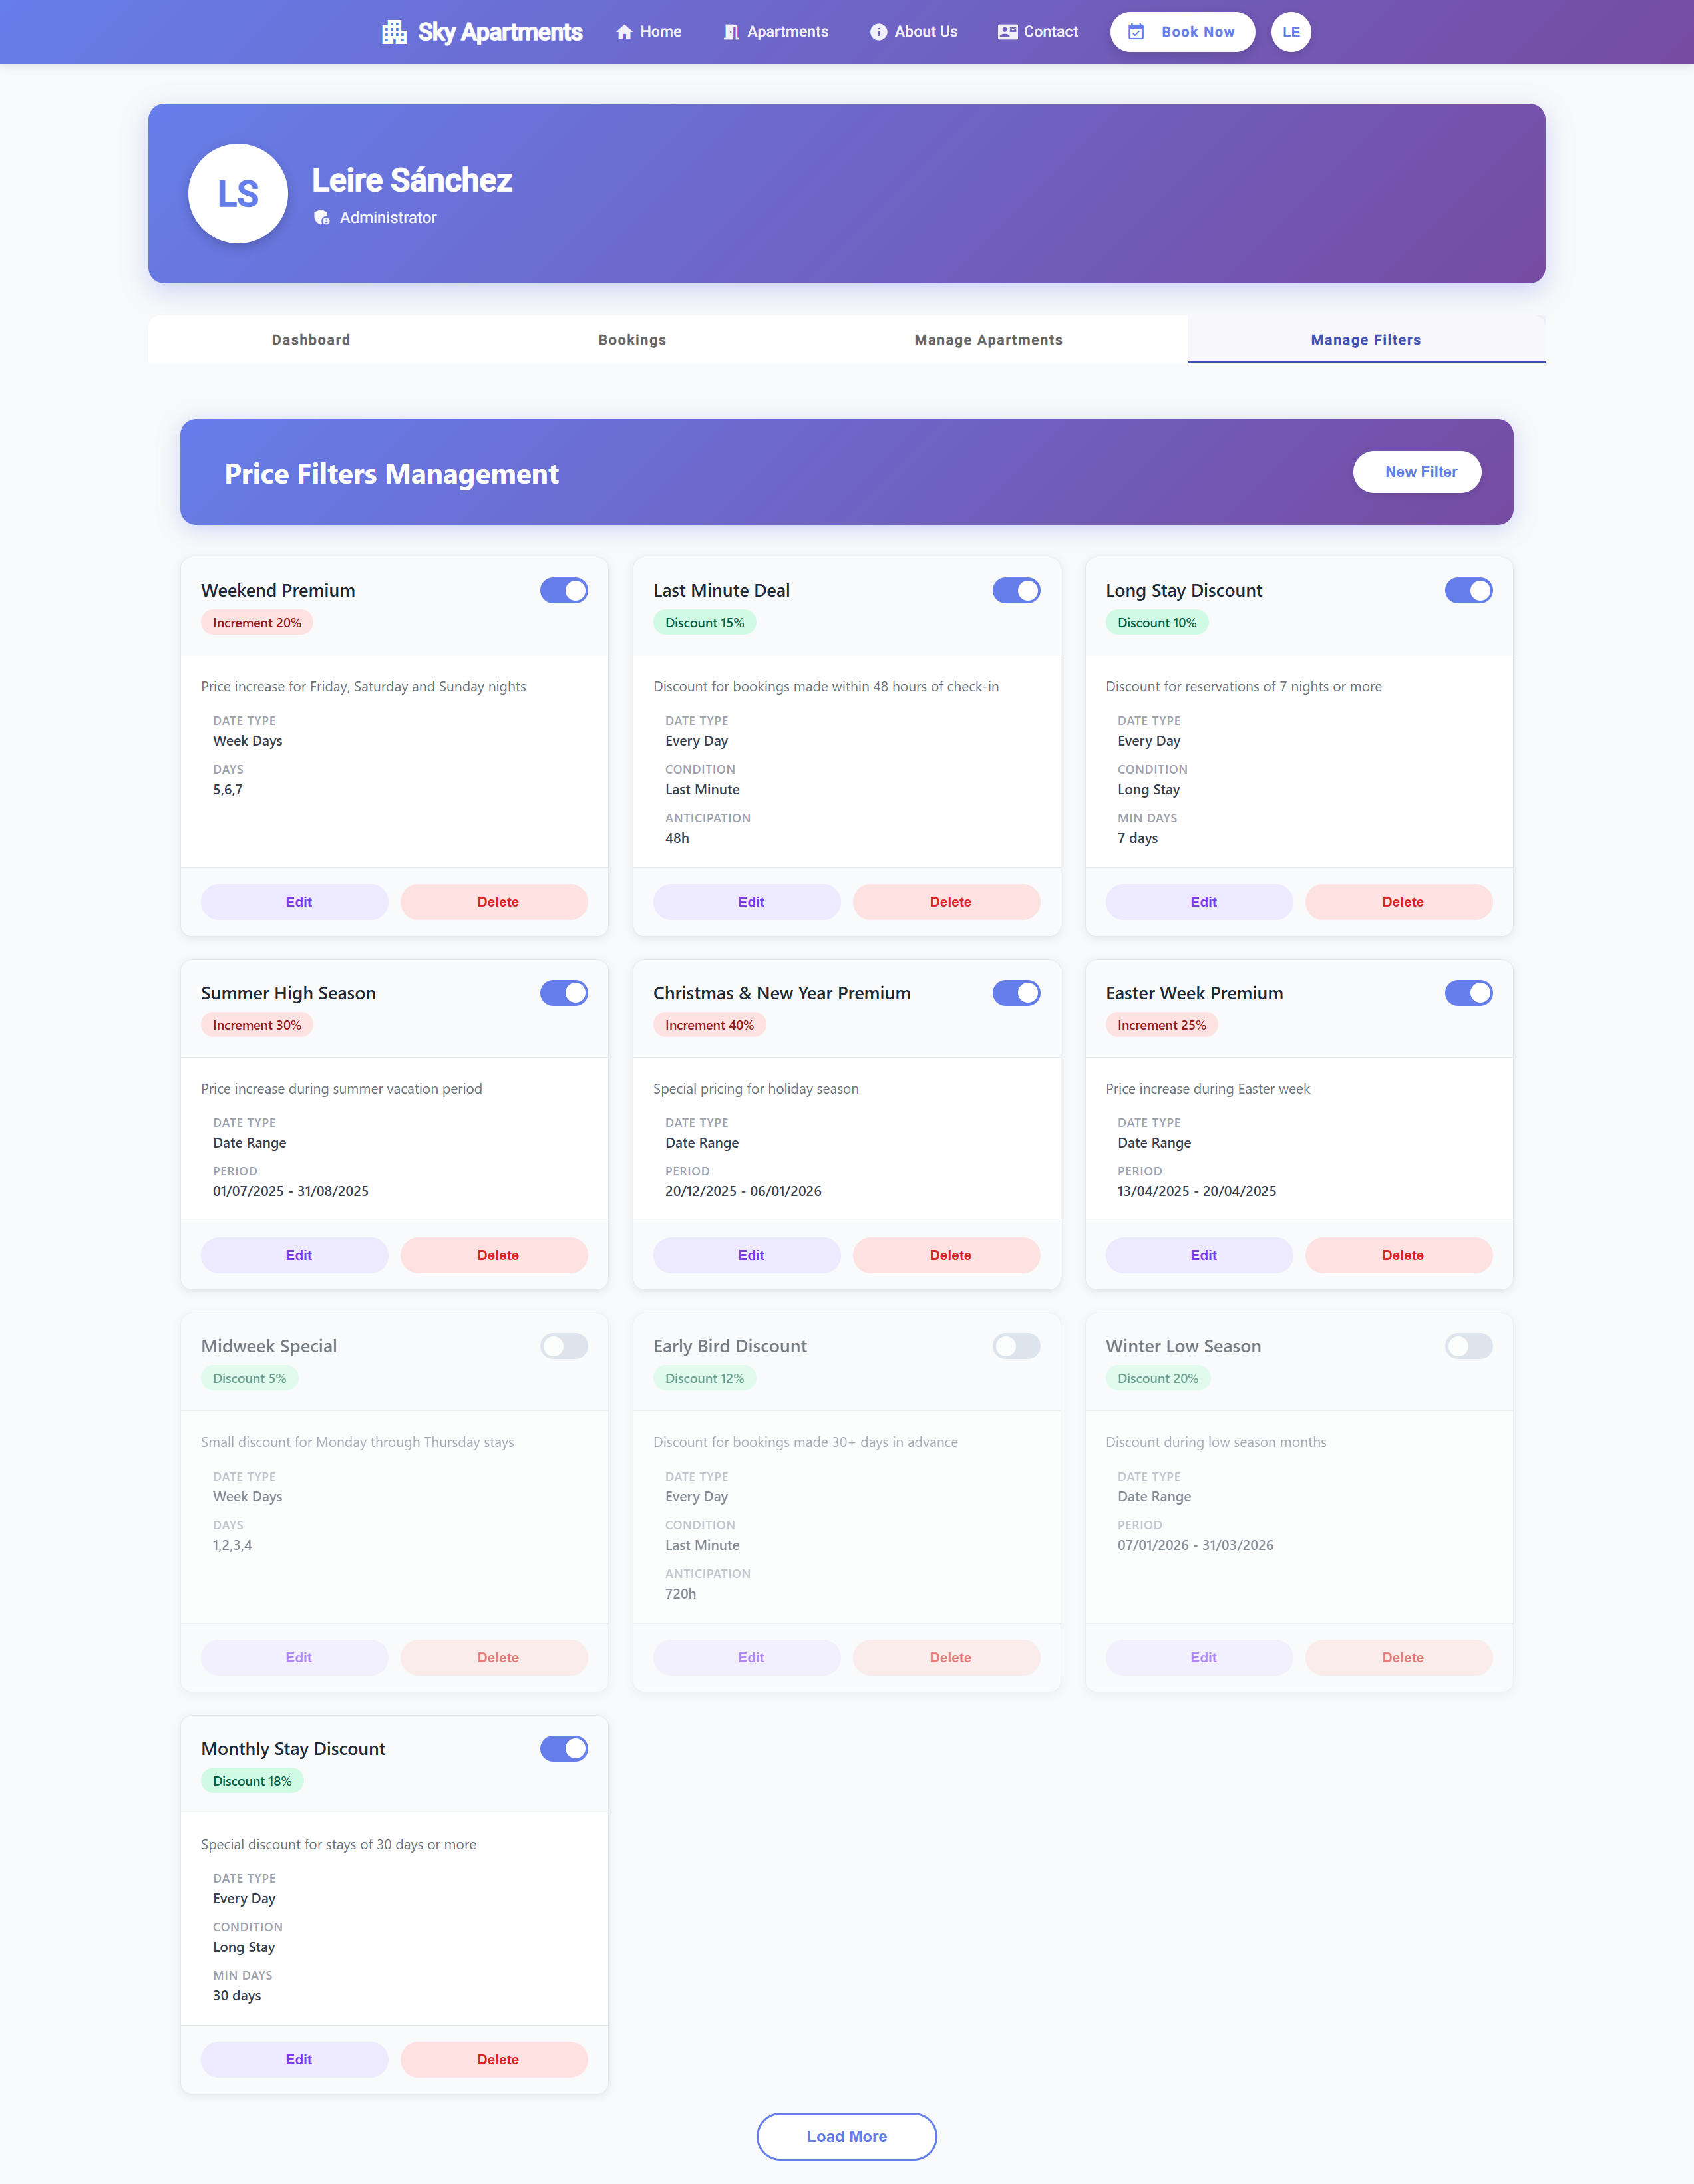
\includegraphics[width=0.9\textwidth]{img/admin_filters_v1.png}
    \caption{Interfaz de gestión y edición de filtros dinámicos de precios.}
    \label{fig:admin_filters}
\end{figure}

\subsection{Administración de Reservas}
Proporciona una vista en forma de lista paginada o calendario de todas las reservas del sistema. Incluye filtros avanzados para buscar reservas por estado, rango de fechas o nombre del apartamento, permitiendo una gestión operativa y eficiente incluso con grandes volúmenes de datos (ver Figura \ref{fig:admin_bookings}).

\begin{figure}[H]
    \centering
    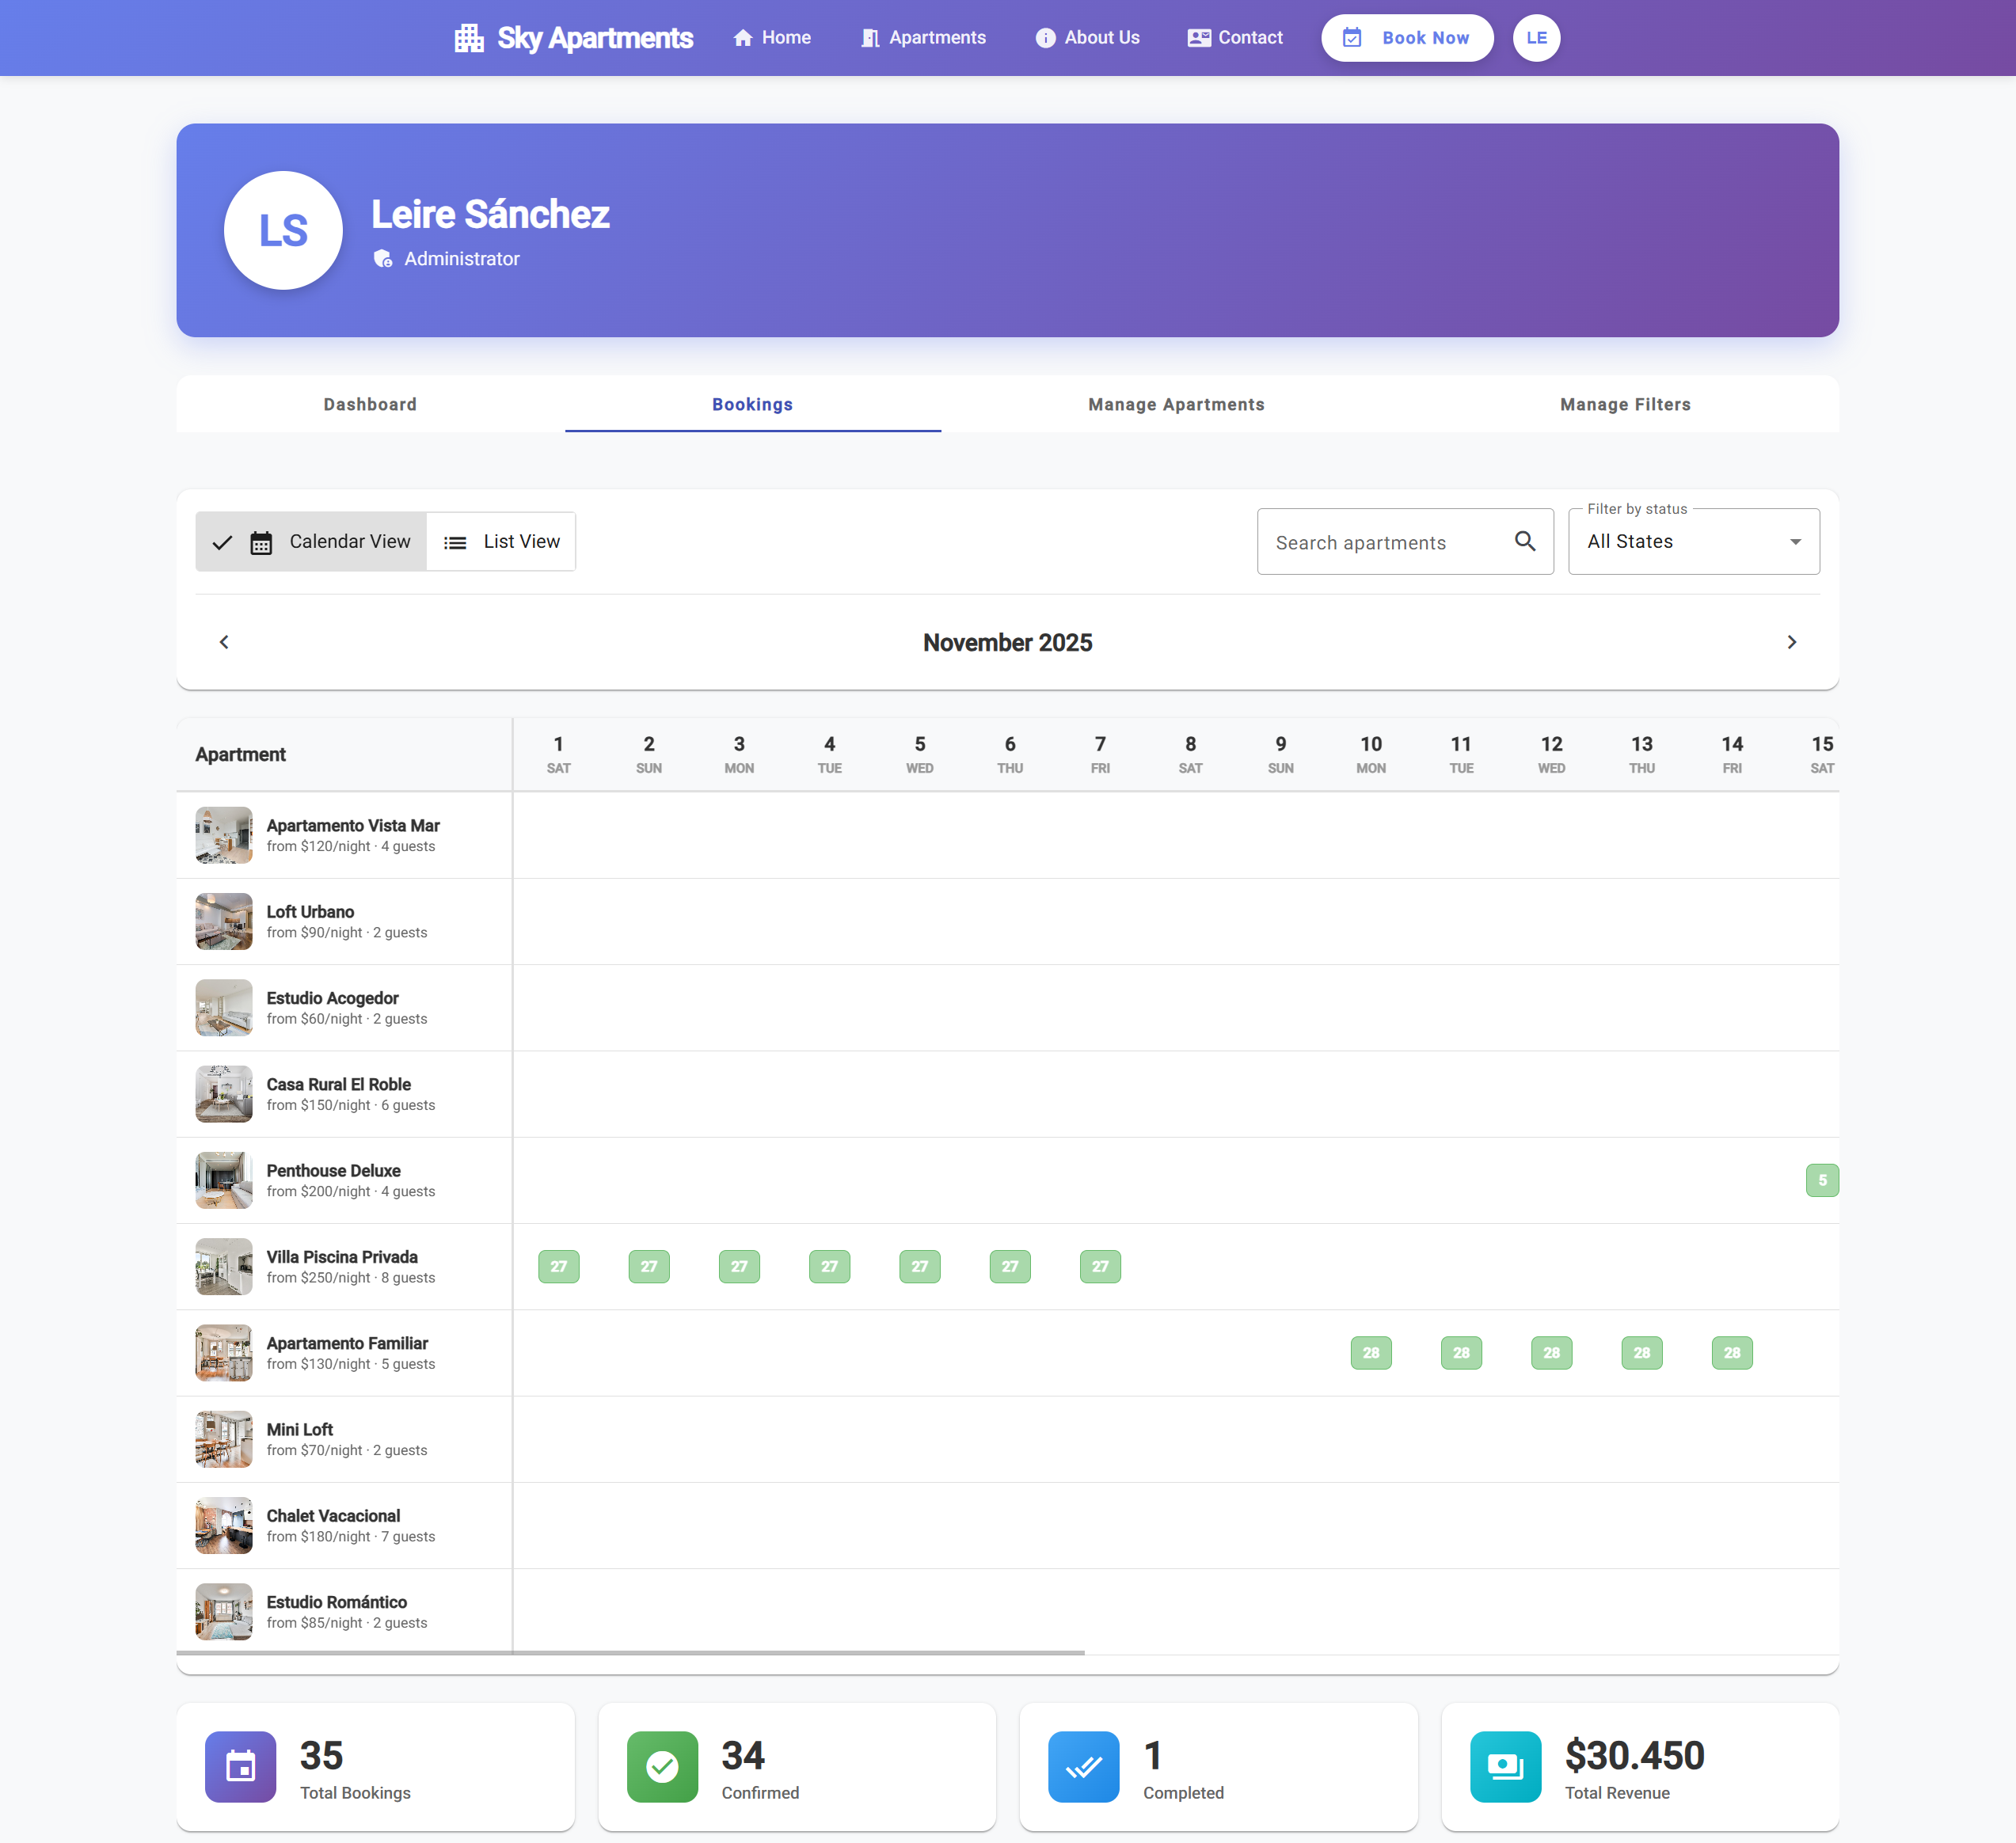
\includegraphics[width=0.9\textwidth]{img/admin_bookings_v1.png}
    \caption{Panel de control para la gestión y seguimiento de todas las reservas.}
    \label{fig:admin_bookings}
\end{figure}


\clearpage
\blankpage

% Capítulo 4
\chapter{Descripción Informática}
\label{sec:descripcionInformatica}

\minitoc
\clearpage

Este capítulo detalla los aspectos informáticos y las decisiones técnicas adoptadas en el desarrollo de \textbf{Sky Apartments}. El código fuente completo está disponible en GitHub:
\newline
\url{https://github.com/codeurjc-students/2025-sky-apartments}.

El sistema sigue una arquitectura distribuida cliente-servidor. El cliente se ha implementado como una \textit{Single Page Application} (SPA) para ofrecer una experiencia de usuario fluida y dinámica. Por su parte, el servidor emplea una arquitectura de \textbf{microservicios} (separando la lógica de usuarios, apartamentos, reservas y reseñas) que se comunican mediante una API REST. Para garantizar un bajo acoplamiento, la capa de datos aplica el patrón de base de datos aislada por servicio.

A modo de síntesis, la configuración técnica del proyecto se resume en la siguiente lista:

\begin{itemize}
    \item \textbf{Tipo:} Aplicación Web SPA, API REST, Arquitectura de Microservicios.
    \item \textbf{Tecnologías:} Java 17, Spring Boot, Spring Cloud, Angular 19, TypeScript, MySQL, MinIO.
    \item \textbf{Herramientas:} Visual Studio Code, Git, GitHub, Maven, Postman.
    \item \textbf{Control de calidad:} Pruebas unitarias, de integración y E2E (JUnit 5, Testcontainers, Karma, Playwright), análisis de cobertura (JaCoCo, Istanbul).
    \item \textbf{Despliegue:} Empaquetado en contenedores con Docker y Docker Compose. Despliegue en la nube mediante Amazon EC2 (AWS). Artefacto distribuido vía DockerHub.
    \item \textbf{Proceso de desarrollo:} Metodología iterativa e incremental, control de versiones (Git), flujos CI/CD automatizados (GitHub Actions).
\end{itemize}

Para abordar estos aspectos en profundidad, el presente capítulo se divide en las siguientes secciones: la \textbf{Sección \ref{sec:tecnologias}} detalla los lenguajes y frameworks de ejecución; la \textbf{Sección \ref{sec:herramientas}} enumera las herramientas de desarrollo empleadas; la \textbf{Sección \ref{sec:arquitectura}} profundiza en el modelo de dominio y la API; la \textbf{Sección \ref{sec:implementacion}} destaca los retos técnicos superados; la \textbf{Sección \ref{sec:control_calidad}} describe la estrategia de pruebas; la \textbf{Sección \ref{sec:despliegue}} detalla el empaquetado en producción; y finalmente, la \textbf{Sección \ref{sec:proceso_desarrollo}} expone la metodología ágil aplicada.

\section{Tecnologías}
\label{sec:tecnologias}

    En esta sección se detallan los lenguajes de programación, frameworks, librerías y sistemas de persistencia que la aplicación utiliza directamente para su ejecución en entornos de producción. La elección de estas tecnologías responde a criterios de escalabilidad, robustez y mantenibilidad, alineándose con los estándares actuales de la industria.

    \subsection{Tecnologías del frontend}
    
        El desarrollo de la interfaz de usuario recae íntegramente sobre tecnologías web modernas orientadas a la construcción de interfaces dinámicas y \textit{responsives}.
        
        \textbf{Angular 19} ~\cite{AngularDocs} \\
        Es una plataforma de código abierto desarrollada y mantenida por Google para la creación de aplicaciones web escalables. En este proyecto, Angular es el pilar fundamental del cliente: gestiona toda la lógica de presentación, el enrutamiento interno entre vistas (catálogo, panel de administración, perfil) y la comunicación HTTP con los microservicios del backend. Su arquitectura basada en componentes y su sistema de inyección de dependencias han permitido estructurar el código de forma modular y reutilizable.
        
        \textbf{TypeScript} ~\cite{TypeScript2014} \\
        Es un superconjunto de JavaScript desarrollado por Microsoft que añade tipado estático opcional. Se utiliza como el lenguaje de programación principal de toda la capa frontend. Su uso en el proyecto ha sido vital para modelar las respuestas de la API mediante interfaces, permitiendo detectar errores de integración en tiempo de compilación y facilitando la refactorización segura del código.
        
        \textbf{RxJS (Reactive Extensions for JavaScript)} ~\cite{RxJS} \\
        Es una librería para programación reactiva que permite componer programas asíncronos mediante secuencias observables. Dada su complejidad y potencia, es una pieza central en el manejo de datos de la aplicación. Se utiliza para gestionar las peticiones asíncronas a la API REST, manejar los eventos de la interfaz de usuario (como los formularios dinámicos de búsqueda) y compartir el estado reactivo entre diferentes componentes sin acoplarlos.
        
        \textbf{HTML5 y CSS3} \\
        Estándares fundamentales de la web utilizados para definir la estructura semántica y el diseño visual de la aplicación, respectivamente. Se han empleado para garantizar un diseño \textit{responsive} que adapte la vista de los apartamentos y calendarios tanto a dispositivos móviles como a resoluciones de escritorio.
        
        \textbf{Chart.js} ~\cite{Chartjs} \textbf{y SweetAlert2} ~\cite{SweetAlert2} \\
        Chart.js es una librería especializada en la visualización gráfica de datos. En el proyecto se utiliza para renderizar los gráficos interactivos (ingresos mensuales, ocupación) del panel de administración. Por su parte, SweetAlert2 es una librería de interfaz de usuario empleada para sustituir los cuadros de diálogo nativos del navegador por ventanas modales personalizadas, mejorando la experiencia de usuario durante confirmaciones críticas (como la cancelación de una reserva).
        
        En la Figura~\ref{fig:stack_frontend} se muestra un resumen visual del stack de tecnologías frontend empleadas en el proyecto.
        \begin{figure}[H]
          \centering
          
\includegraphics[width=0.8\textwidth,clip=true]{img/Diapositiva1.PNG}
          \caption{Tecnologías del frontend empleadas en el proyecto.}
          \label{fig:stack_frontend}
        \end{figure}
    
    \subsection{Tecnologías del Backend}
    
        El servidor se ha construido priorizando el rendimiento, la seguridad y la capacidad de operar en un entorno distribuido.
        
        \textbf{Java 17} ~\cite{java} \\
        Lenguaje de programación orientado a objetos, de propósito general y fuertemente tipado. La versión 17 (Long-Term Support) se utiliza como el motor principal de toda la lógica del servidor, aprovechando sus características modernas (como los \textit{records}) para crear modelos de datos inmutables en la transferencia de información.
        
        \textbf{Spring Boot} ~\cite{SpringBootDocs} \\
        Es el framework base sobre el que se construyen todos los microservicios del sistema. Simplifica radicalmente la configuración de aplicaciones Java de grado empresarial. En el proyecto se utilizan varios de sus submódulos principales:
        \begin{itemize}
            \item \textbf{Spring Web} ~\cite{SpringWeb}\textbf{:} Utilizado para exponer los endpoints de la API REST y procesar las peticiones HTTP entrantes.
            \item \textbf{Spring Data JPA} ~\cite{SpringDataJPA}\textbf{:} Utilizado como capa de abstracción sobre Hibernate para facilitar el acceso y manipulación de los datos en MySQL mediante el patrón Repositorio.
            \item \textbf{Spring Security} ~\cite{SpringSecurity}\textbf{:} Empleado para gestionar la autenticación de usuarios y proteger los recursos mediante control de acceso basado en roles (RBAC).
        \end{itemize}
        
        \textbf{Spring Cloud (Netflix Eureka y \textit{API Gateway})} ~\cite{SpringCloud} ~\cite{SpringCloudNetflix} ~\cite{SpringCloudGateway} \\
        Conjunto de herramientas para el desarrollo de sistemas distribuidos. En este proyecto, Netflix Eureka se utiliza como servidor de descubrimiento dinámico, permitiendo que los microservicios se localicen entre sí sin depender de direcciones IP fijas. Spring Cloud Gateway se utiliza como el punto de entrada único de la aplicación, enrutando las peticiones externas hacia el microservicio correspondiente y actuando como barrera de seguridad perimetral.
        
        \textbf{JSON Web Tokens (JWT)} ~\cite{RFC7519} \\
        Estándar abierto (RFC 7519) que define un formato compacto para transmitir información de forma segura entre las partes como un objeto JSON. Se utiliza como el núcleo del sistema de autenticación sin estado (\textit{stateless}). El microservicio de usuarios emite un JWT firmado tras un login exitoso, y este token se utiliza en las peticiones posteriores para validar la identidad del cliente.
        
        \textbf{OpenAPI 3.0 (SpringDoc)} ~\cite{OpenAPI} ~\cite{SpringDoc} \\
        Especificación estándar para la descripción de interfaces de programación (APIs). Mediante la librería SpringDoc, se utiliza para autogenerar una documentación interactiva y estandarizada de todos los endpoints de los microservicios, facilitando enormemente la integración entre el equipo de frontend y el de backend.
    
    \subsection{Persistencia y Comunicaciones}
    
        Para el almacenamiento de estado y la comunicación asíncrona con los usuarios, el sistema se apoya en tecnologías consolidadas (ver Figura~\ref{fig:stack_persistencia}).
        
        \textbf{MySQL} ~\cite{MySQLManual} \\
        Sistema de gestión de bases de datos relacionales (SGBD) de código abierto. Se utiliza para la persistencia transaccional de los datos del negocio (usuarios, reservas, apartamentos). Siguiendo el patrón de arquitectura adoptado, cada microservicio gestiona su propio esquema de base de datos MySQL independiente para evitar el acoplamiento de datos.
        
        \textbf{MinIO} ~\cite{MinIO} \\
        Servidor de almacenamiento de objetos de alto rendimiento, compatible con el protocolo Amazon S3. A diferencia de las bases de datos relacionales, MinIO está optimizado para datos no estructurados. En el proyecto, se utiliza exclusivamente como el repositorio centralizado para almacenar y servir las imágenes en alta resolución del catálogo de apartamentos.
        
        \textbf{Spring Boot Starter Mail} ~\cite{SpringMail} \\
        Módulo de integración de Spring que proporciona soporte para el envío de correos electrónicos. Se utiliza en el microservicio de reservas para establecer comunicación vía protocolo SMTP con los clientes, enviando automáticamente correos electrónicos HTML transaccionales (confirmaciones de reserva, cancelaciones y recordatorios).
        
        \begin{figure}[H]
          \centering
          
\includegraphics[width=0.8\textwidth,clip=true]{img/Diapositiva3.PNG}
          \caption{Tecnologías de persistencia y almacenamiento de objetos.}
          \label{fig:stack_persistencia}
        \end{figure}


\section{Herramientas}
\label{sec:herramientas}

    En esta sección se describen los Entornos de Desarrollo Integrado (IDE) y las herramientas auxiliares empleadas a lo largo del ciclo de vida del proyecto. A diferencia de las tecnologías detalladas en la sección anterior, estas herramientas no se ejecutan en el entorno de producción, sino que conforman el ecosistema de trabajo local necesario para la escritura de código, gestión de versiones, construcción del software y pruebas manuales.
    
    \subsection{Entorno de Desarrollo Integrado (IDE)}
    
    \textbf{Visual Studio Code (VS Code)} ~\cite{VSCode} \\
    Para la escritura y edición del código fuente se ha seleccionado Visual Studio Code, un editor de código fuente ligero, multiplataforma y altamente personalizable desarrollado por Microsoft. A diferencia de enfoques tradicionales donde se utiliza un IDE pesado para el backend (como IntelliJ IDEA o Eclipse) y otro distinto para el frontend, VS Code ha permitido unificar todo el flujo de trabajo en una única herramienta.
    \begin{itemize}
        \item \textbf{Uso en el proyecto:} Se ha utilizado de forma simultánea tanto para el desarrollo de la \textit{Single Page Application} en Angular como para la implementación de los microservicios distribuidos en Spring Boot.
        \item \textbf{Extensiones clave:} Su extenso ecosistema de extensiones ha sido fundamental para adaptar el editor a las necesidades del proyecto. Se han empleado paquetes como \textit{Extension Pack for Java} y \textit{Spring Boot Tools} para habilitar el autocompletado inteligente, la navegación por el código y la gestión dinámica de dependencias en el backend. Para el frontend, se ha integrado \textit{Angular Language Service}, proporcionando análisis estático y validación de sintaxis en las plantillas HTML en tiempo real.
    \end{itemize}
    
    \subsection{Control de Versiones y Trabajo Colaborativo}
    
    \textbf{Git} ~\cite{Git} \\
    Sistema de control de versiones distribuido de código abierto, diseñado para manejar proyectos de software con rapidez y eficiencia, permitiendo un seguimiento minucioso del histórico de modificaciones.
    \begin{itemize}
        \item \textbf{Uso en el proyecto:} Ha sido la herramienta fundamental para mantener un registro histórico de todos los cambios en el código fuente. Ha permitido estructurar el trabajo mediante el uso de ramas (\textit{branches}), aislando el desarrollo de nuevas funcionalidades y la corrección de errores (\textit{feature branches}) del código estable principal. Esto ha facilitado una experimentación segura, garantizando la posibilidad de revertir cambios (\textit{rollbacks}) en caso de errores críticos.
    \end{itemize}
    
    \textbf{GitHub y GitHub Projects} ~\cite{GitHub} ~\cite{GitHubProjects} \\
    Plataforma de alojamiento basada en la nube para el control de versiones y la colaboración mediante Git.
    \begin{itemize}
        \item \textbf{Uso en el proyecto:} Además de actuar como el repositorio remoto central (\textit{origin}) donde se aloja y respalda el código fuente del TFG, la plataforma ha sido el núcleo operativo de la gestión organizativa. Mediante \textbf{GitHub Projects}, se implementó un tablero de gestión visual tipo Kanban que permitió realizar un seguimiento del progreso. Las tareas, errores detectados y nuevas características se definieron utilizando \textit{GitHub Issues}, vinculándolas directamente a los \textit{commits} correspondientes para garantizar la trazabilidad del código.
    \end{itemize}
    
    \subsection{Gestión de Dependencias y Construcción}
    
    \textbf{Apache Maven} ~\cite{Maven} \\
    Herramienta de gestión y comprensión de proyectos de software basada en el concepto de Modelo de Objetos de Proyecto (POM).
    \begin{itemize}
        \item \textbf{Uso en el proyecto:} En el ecosistema del backend, Maven se ha encargado de la gestión de todas las librerías externas de Spring Boot y Spring Cloud, resolviendo y descargando automáticamente las dependencias transitivas. Asimismo, se ha utilizado para estandarizar el ciclo de vida de construcción del software en Java: desde la limpieza de ejecutables anteriores (\texttt{clean}), pasando por la compilación (\texttt{compile}) y ejecución de pruebas (\texttt{test}), hasta el empaquetado final de cada microservicio en un archivo ejecutable (\texttt{package}).
    \end{itemize}
    
    \textbf{Node Package Manager (npm)} ~\cite{npm} \\
    Es el gestor de paquetes predeterminado para el entorno de ejecución de JavaScript Node.js. Aunque el proyecto no despliega un servidor Node.js en producción, npm es un requisito arquitectónico imprescindible para el desarrollo moderno del frontend.
    \begin{itemize}
        \item \textbf{Uso en el proyecto:} Se ha utilizado para instalar, actualizar y gestionar todas las dependencias del ecosistema Angular (como RxJS, Chart.js o SweetAlert2), manteniendo la coherencia de versiones a través del archivo \texttt{package.json}. Además, npm se encarga de lanzar los \textit{scripts} de desarrollo local, la ejecución de las suites de pruebas del cliente web y el proceso final de compilación e instanciación de los archivos estáticos para producción (\textit{build}).
    \end{itemize}
    
    \subsection{Pruebas de Integración y Documentación de API}
    
    \textbf{Postman} ~\cite{Postman} \\
    Plataforma colaborativa para el desarrollo, prueba y consumo de APIs. Proporciona una interfaz gráfica intuitiva para construir y ejecutar peticiones HTTP complejas.
    \begin{itemize}
        \item \textbf{Uso en el proyecto:} Ha sido una herramienta indispensable durante la fase de desarrollo del servidor backend, operando de puente antes de que existiera una interfaz gráfica en el cliente Angular. Se han creado colecciones de Postman organizadas por dominio (Usuarios, Apartamentos, Reservas, Reseñas). El uso de variables de entorno dentro de Postman ha permitido almacenar de forma dinámica los \textit{tokens} JWT tras la autenticación, facilitando la prueba manual de cada \textit{endpoint} privado simulando el comportamiento del frontend y verificando la exactitud de las respuestas JSON.
    \end{itemize}

    En la Figura~\ref{fig:stack_desarrollo} se ofrece una visión conjunta de las principales herramientas de desarrollo empleadas a lo largo del proyecto.

    \begin{figure}[H]
      \centering
      
\includegraphics[width=0.8\textwidth,clip=true]{img/Diapositiva6.PNG}
      \caption{Herramientas de desarrollo: Git y GitHub (arriba); Apache Maven y Visual Studio Code (abajo); con Postman en el centro.}
      \label{fig:stack_desarrollo}
    \end{figure}


\section{Arquitectura}
    \label{sec:arquitectura}
    En esta sección se presenta la arquitectura del sistema \textbf{Sky Apartments}, describiendo los componentes principales, las relaciones entre ellos y las decisiones de diseño adoptadas.

    La plataforma sigue una arquitectura fuertemente desacoplada donde el cliente web (frontend) y el servidor (backend) evolucionan de forma independiente, comunicándose exclusivamente a través de una API REST.

    \subsection{Despliegue}
        La arquitectura de despliegue de Sky Apartments está basada íntegramente en contenedores, organizando el sistema en diferentes procesos independientes que interactúan a través de una red virtual privada (ver Figura \ref{fig:arquitectura_despliegue}). 

        \textbf{Procesos independientes:}
        El sistema se compone de los siguientes nodos o contenedores aislados:
        \begin{itemize}
            \item \textbf{\textit{API Gateway} y Frontend:} Actúa como punto único de entrada, sirviendo los archivos estáticos de Angular y enrutando las peticiones de la API.
            \item \textbf{Microservicios de Dominio:} Cuatro procesos Java independientes (\textit{User Service}, \textit{Apartment Service}, \textit{Booking Service}, \textit{Review Service}) que ejecutan la lógica de negocio.
            \item \textbf{Infraestructura de Soporte:} Un contenedor para \textit{Eureka Server} (descubrimiento de servicios), uno para \textit{Jaeger} (trazabilidad distribuida) y otro para \textit{MinIO} (almacenamiento de objetos S3).
            \item \textbf{Capa de Persistencia:} Un único motor \textbf{MySQL 8.0} que aloja cuatro esquemas de base de datos independientes (\texttt{usersdb}, \texttt{apartmentsdb}, \texttt{bookingsdb}, \texttt{reviewsdb}), preservando el aislamiento lógico de datos que exige el patrón \textit{Database per Service}~\cite[Cap.~5]{richardson2018}.
        \end{itemize}

        \textbf{Protocolos de comunicación:}
        La interacción entre estos procesos se realiza mediante un conjunto de protocolos estandarizados:
        \begin{itemize}
            \item \textbf{HTTPS (Puerto 443):} Único protocolo expuesto al exterior para la comunicación encriptada entre el navegador del cliente y el \textit{API Gateway}.
            \item \textbf{HTTP/REST:} Utilizado para la comunicación interna síncrona entre microservicios (mediante \textit{Feign Clients}) y para el registro en Eureka.
            \item \textbf{JDBC:} Protocolo utilizado para la conexión entre cada microservicio Java y su respectiva base de datos MySQL sobre la red privada de Docker.
            \item \textbf{S3 Protocol:} Utilizado por el \textit{Apartment Service} para gestionar la carga y descarga de imágenes en el servidor MinIO.
        \end{itemize}

        \begin{figure}[!h]
            \centering
            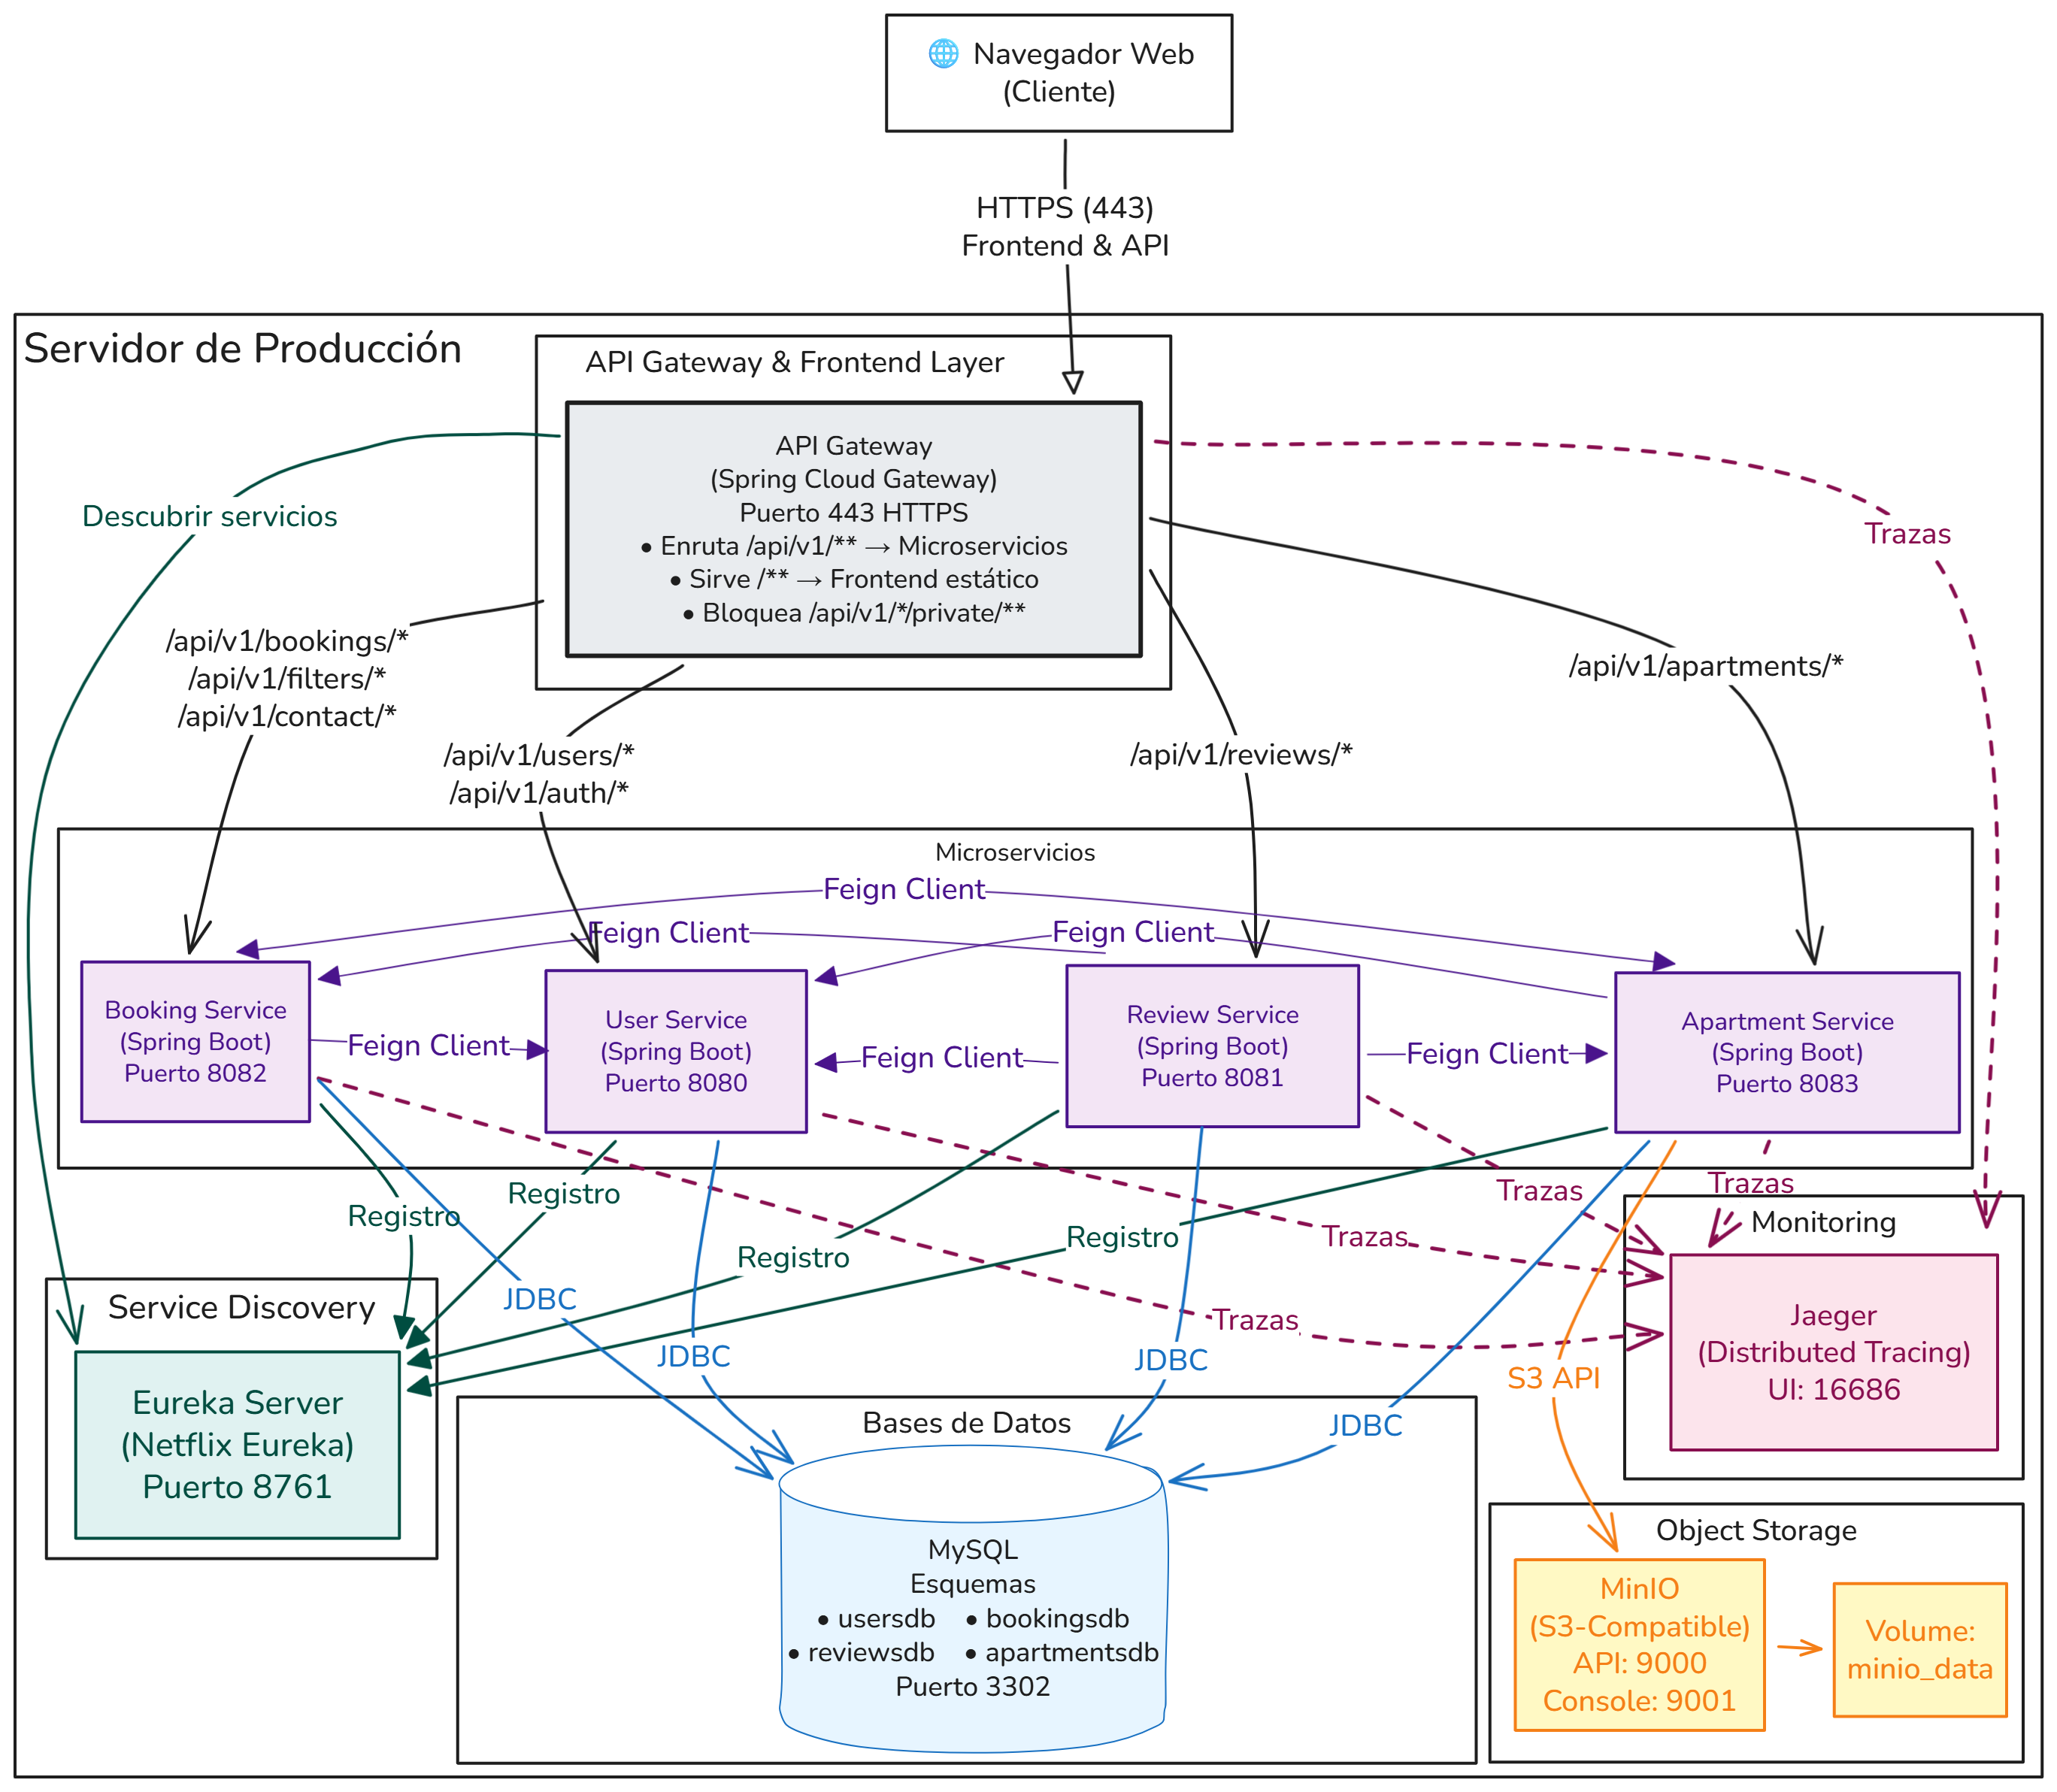
\includegraphics[width=1.2\textwidth, clip=true]{img/deployment_architecture.png}
            \caption{Arquitectura de despliegue: procesos contenerizados, puertos y flujos de comunicación.}
            \label{fig:arquitectura_despliegue}
        \end{figure}

    \subsection{Modelo del Dominio}
        El modelo de dominio representa las entidades principales del sistema, sus atributos clave y las relaciones que definen la lógica del negocio. Debido a la naturaleza distribuida de los microservicios, las relaciones entre dominios distintos no se materializan mediante claves foráneas (\textit{Foreign Keys}) tradicionales en la base de datos, sino a través de referencias lógicas (identificadores) que se validan mediante peticiones REST.

        Las entidades persistentes del sistema son (ver Figura \ref{fig:modelo_dominio}):
        \begin{itemize}
            \item \textbf{User (Usuario):} Representa a los actores del sistema. Contiene atributos como \texttt{id}, \texttt{email} (único), \texttt{password} (encriptada), \texttt{firstName}, \texttt{lastName} y \texttt{role} (USER o ADMIN).
            \item \textbf{Apartment (Apartamento):} Núcleo del catálogo. Sus atributos incluyen \texttt{id}, \texttt{name}, \texttt{description}, \texttt{basePrice}, \texttt{maxGuests}, y una lista de comodidades (\texttt{amenities}) y referencias a imágenes almacenadas en MinIO.
            \item \textbf{Booking (Reserva):} Registra los alquileres. Relaciona un \texttt{userId} y un \texttt{apartmentId}. Incluye \texttt{checkInDate}, \texttt{checkOutDate}, \texttt{totalPrice}, \texttt{status} (CONFIRMED, CANCELLED, COMPLETED) y \texttt{guestCount}.
            \item \textbf{Review (Reseña):} Almacena el \textit{feedback} de los usuarios. Vincula un \texttt{userId} con un \texttt{apartmentId} e incluye \texttt{rating} (1-5), \texttt{comment} y \texttt{createdAt}.
            \item \textbf{Filter (Regla de Precio):} Entidad administrable que define las reglas de precios dinámicos, incluyendo \texttt{name}, \texttt{increment} (booleano), \texttt{value} (porcentaje) y condiciones temporales.
        \end{itemize}

        \begin{figure}[H]
            \centering
            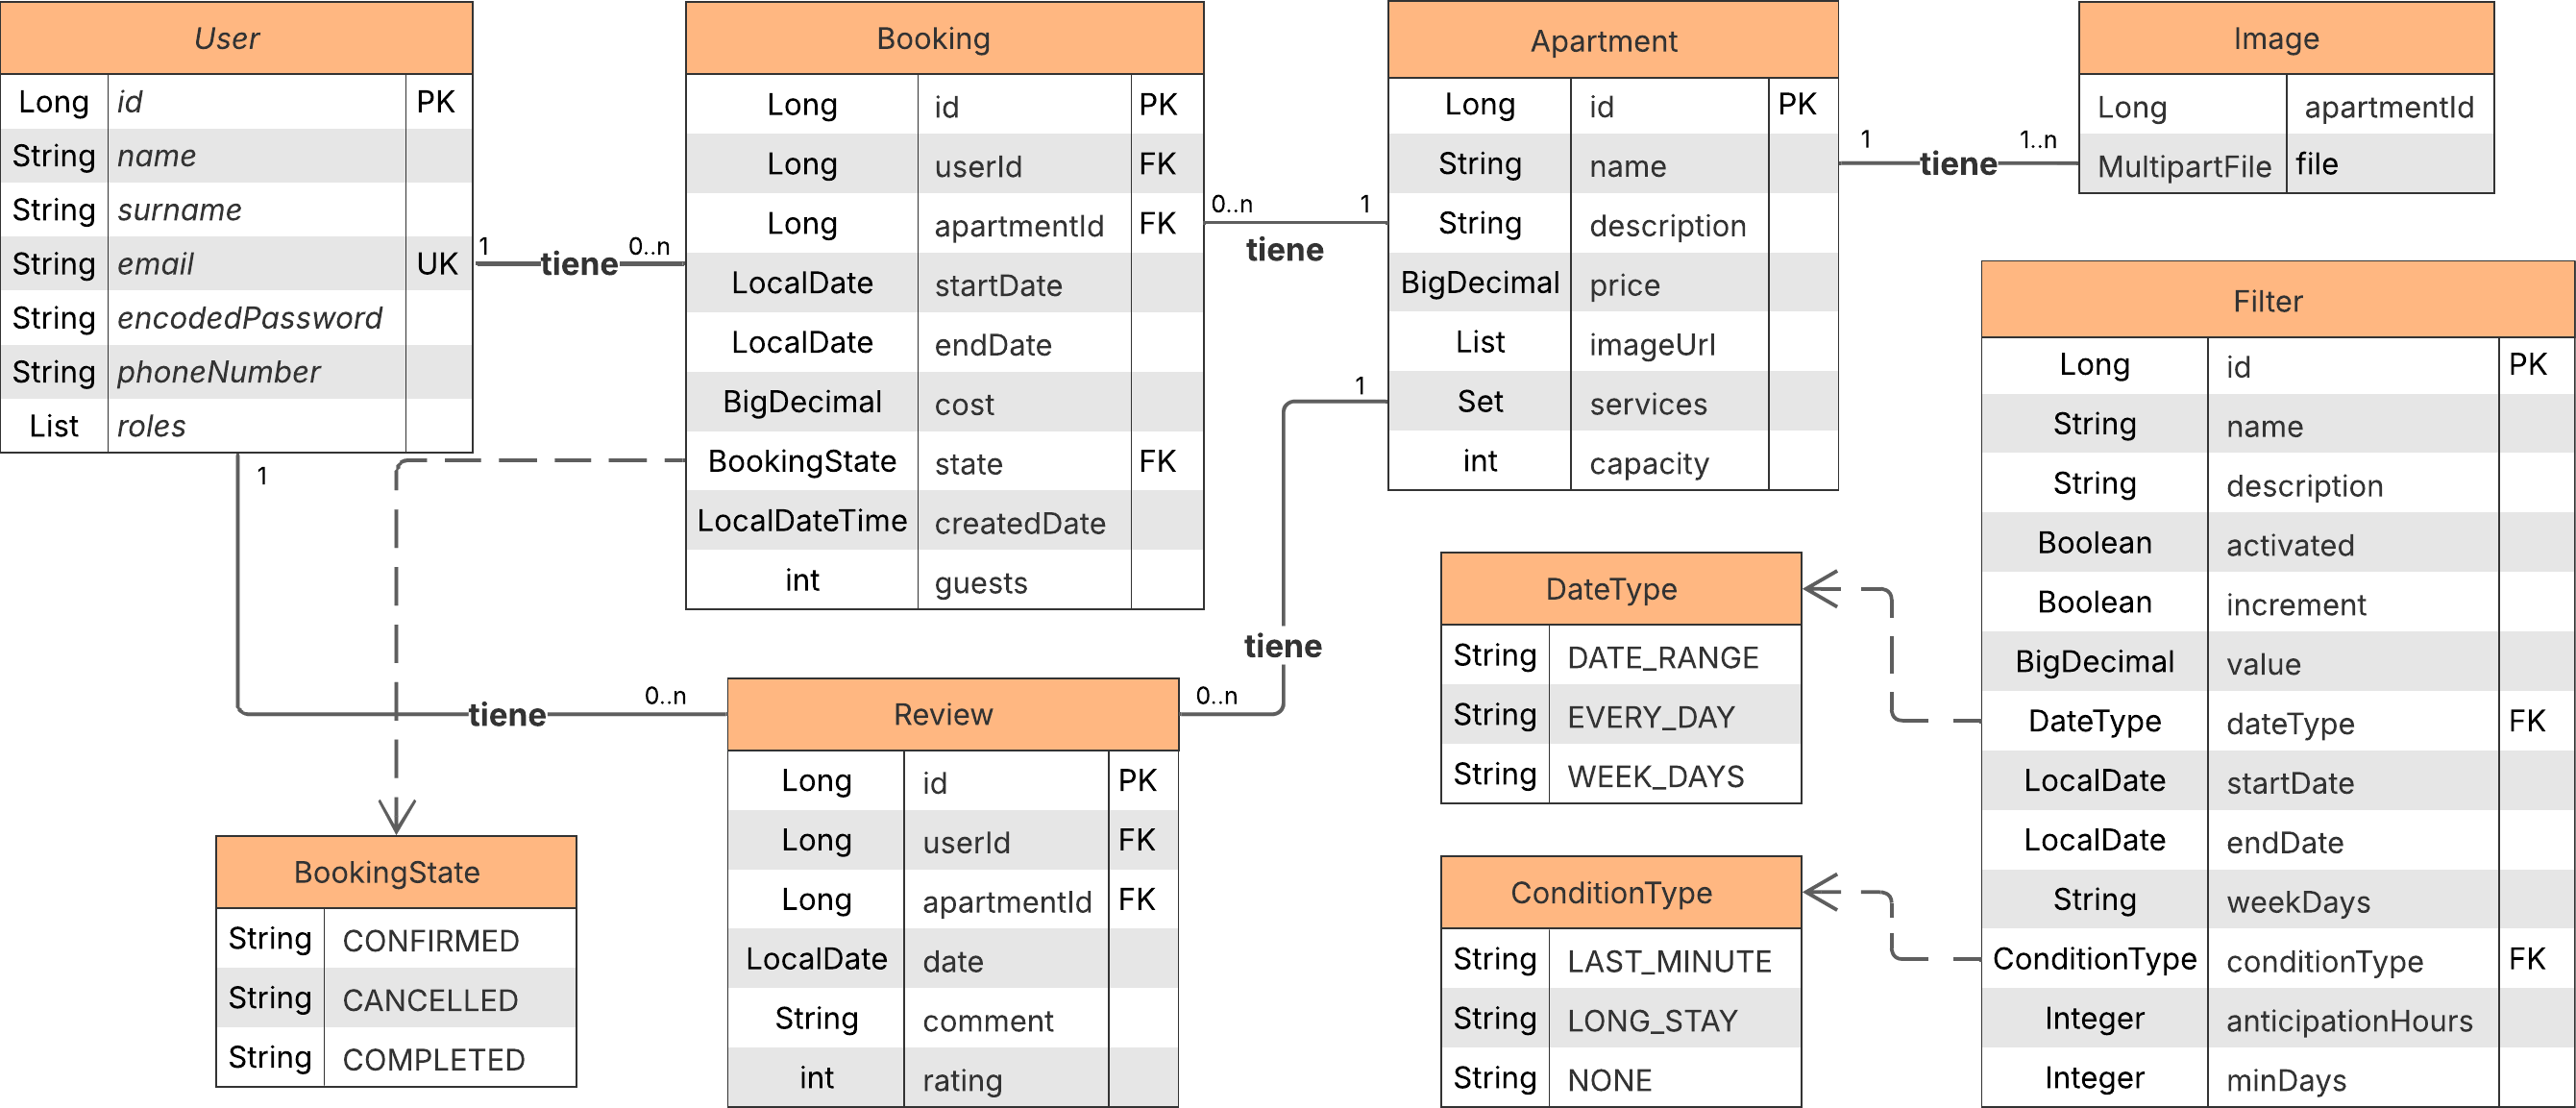
\includegraphics[width=1\textwidth, clip=true]{img/diagrama_entidad.png}
            \caption{Modelo de dominio lógico del sistema Sky Apartments.}
            \label{fig:modelo_dominio}
        \end{figure}

    \subsection{API REST}
        El sistema expone una API RESTful documentada bajo el estándar OpenAPI 3.0. Todas las peticiones del cliente se canalizan a través del \textit{API Gateway} mediante el prefijo \texttt{/api/v1/}. A continuación, se describen a alto nivel los recursos públicos principales, detallando su estructura JSON y las operaciones disponibles agrupadas por método HTTP. Se han omitido de forma deliberada los \textit{endpoints} internos (rutas \texttt{/private/}) diseñados exclusivamente para la comunicación síncrona entre microservicios.

        \subsubsection{Recurso Apartments}
        Gestiona el catálogo de alojamientos, sus características y la comprobación de su disponibilidad.
        \begin{lstlisting}[basicstyle=\jsonbasicfont,frame=single,backgroundcolor=\color{white},rulecolor=\color{black},framerule=0.5pt,numbers=none]
        {
        "id": 1,
        "name": "Ocean View Penthouse",
        "description": "Luxury apartment with panoramic sea views.",
        "price": 150.00,
        "capacity": 4,
        "services": ["WIFI", "TERRACE", "POOL"],
        "imagesUrl": ["https://minio.../image1.jpg"]
        }
        \end{lstlisting}

        \textbf{Operaciones}
        \begin{itemize}
            \item \textbf{GET /api/v1/apartments/} - Obtiene el listado completo paginado de apartamentos.
            \item \textbf{GET /api/v1/apartments/\{id\}} - Obtiene los detalles completos de un apartamento específico.
            \item \textbf{GET /api/v1/apartments/search} - Busca apartamentos filtrando por servicios, capacidad y fechas de disponibilidad.
            \item \textbf{GET /api/v1/apartments/services} - Devuelve el conjunto de todos los servicios/comodidades posibles.
            \item \textbf{GET /api/v1/apartments/\{id\}/availability} - Comprueba si un apartamento está disponible en un rango de fechas.
            \item \textbf{POST /api/v1/apartments} - Crea un nuevo apartamento, soportando subida de imágenes \textit{Multipart} (Requiere rol ADMIN).
            \item \textbf{PUT /api/v1/apartments/\{id\}} - Actualiza la información de un apartamento existente (Requiere rol ADMIN).
            \item \textbf{DELETE /api/v1/apartments/\{id\}} - Elimina un apartamento del catálogo (Requiere rol ADMIN).
        \end{itemize}

    \subsubsection{Recurso Bookings}
        Gestiona el ciclo de vida de las reservas y se encarga del cálculo del precio final basado en fechas.
        \begin{lstlisting}[basicstyle=\jsonbasicfont,frame=single,backgroundcolor=\color{white},rulecolor=\color{black},framerule=0.5pt,numbers=none]
        {
        "id": 1024,
        "userId": 5,
        "apartmentId": 1,
        "startDate": "2026-08-15",
        "endDate": "2026-08-20",
        "guests": 2,
        "cost": 850.50,
        "state": "CONFIRMED",
        "createdDate": "2026-07-01T10:00:00Z"
        }
        \end{lstlisting}

        \textbf{Operaciones}
        \begin{itemize}
            \item \textbf{GET /api/v1/bookings/user/\{userId\}} - Obtiene el historial de reservas paginado de un usuario.
            \item \textbf{GET /api/v1/bookings/apartment/\{apartmentId\}} - Obtiene las reservas asociadas a un apartamento específico.
            \item \textbf{POST /api/v1/bookings} - Crea y confirma una nueva reserva.
            \item \textbf{PUT /api/v1/bookings/\{bookingId\}/dates} - Modifica las fechas de entrada y salida de una reserva existente.
            \item \textbf{DELETE /api/v1/bookings/\{bookingId\}} - Cancela una reserva activa.
        \end{itemize}

    \subsubsection{Recurso Filters}
        Administra el motor de reglas de precios dinámicos aplicables a las reservas.
        \begin{lstlisting}[basicstyle=\jsonbasicfont,frame=single,backgroundcolor=\color{white},rulecolor=\color{black},framerule=0.5pt,numbers=none]
        {
        "id": 1,
        "name": "Weekend Premium",
        "description": "Increment for weekend stays",
        "activated": true,
        "increment": true,
        "value": 15.00,
        "dateType": "WEEK_DAYS",
        "weekDays": "5,6,7",
        "conditionType": "NONE"
        }
        \end{lstlisting}

        \textbf{Operaciones}
        \begin{itemize}
            \item \textbf{GET /api/v1/filters} - Obtiene el listado paginado de todas las reglas configuradas.
            \item \textbf{GET /api/v1/filters/applicable} - Calcula y devuelve qué reglas de precio aplicarían para un rango de fechas concreto.
            \item \textbf{POST /api/v1/filters} - Crea una nueva regla de precios dinámica (Requiere rol ADMIN).
            \item \textbf{PUT /api/v1/filters/\{id\}} - Modifica la configuración de una regla existente (Requiere rol ADMIN).
            \item \textbf{DELETE /api/v1/filters/\{id\}} - Elimina una regla del sistema (Requiere rol ADMIN).
        \end{itemize}

    \subsubsection{Recurso Users y Auth}
        Gestiona la identidad de los clientes, sus perfiles y el proceso de autenticación.
        \begin{lstlisting}[basicstyle=\jsonbasicfont,frame=single,backgroundcolor=\color{white},rulecolor=\color{black},framerule=0.5pt,numbers=none]
        {
        "id": 5,
        "name": "Carlos",
        "surname": "García",
        "email": "cliente@example.com",
        "phoneNumber": "600000000",
        "roles": ["ROLE_USER"]
        }
        \end{lstlisting}

        \textbf{Operaciones de Usuario}
        \begin{itemize}
            \item \textbf{GET /api/v1/users/me} - Obtiene el perfil completo del usuario autenticado actual.
            \item \textbf{GET /api/v1/users/\{id\}} - Obtiene un usuario específico por su ID.
            \item \textbf{POST /api/v1/users} - Registra un nuevo usuario en el sistema.
            \item \textbf{PUT /api/v1/users/\{id\}} - Actualiza la información personal de un usuario.
            \item \textbf{DELETE /api/v1/users/\{id\}} - Elimina a un usuario del sistema.
        \end{itemize}

        \textbf{Operaciones de Autenticación}
        \begin{itemize}
            \item \textbf{POST /api/v1/auth/login} - Valida credenciales y emite las cookies seguras con los \textit{Auth} y \textit{Refresh tokens}.
            \item \textbf{POST /api/v1/auth/refresh} - Renueva el \textit{token} de acceso caducado utilizando el \textit{Refresh token} de la cookie.
            \item \textbf{POST /api/v1/auth/logout} - Invalida la sesión actual y limpia las cookies del navegador.
        \end{itemize}

    \subsubsection{Recurso Reviews}
        Centraliza el sistema de valoraciones y \textit{feedback} de los huéspedes.
        \begin{lstlisting}[basicstyle=\jsonbasicfont,frame=single,backgroundcolor=\color{white},rulecolor=\color{black},framerule=0.5pt,numbers=none]
        {
        "id": 42,
        "userId": 5,
        "userName": "Carlos G.",
        "apartmentId": 1,
        "date": "2026-08-21",
        "comment": "Estancia inolvidable, todo impecable.",
        "rating": 5
        }
        \end{lstlisting}

        \textbf{Operaciones}
        \begin{itemize}
            \item \textbf{GET /api/v1/reviews/apartment/\{apartmentId\}} - Obtiene la lista paginada de reseñas publicadas en un apartamento.
            \item \textbf{GET /api/v1/reviews/apartment/\{apartmentId\}/rating} - Calcula y devuelve la nota media global de un apartamento.
            \item \textbf{GET /api/v1/reviews/can-review} - Verifica si un usuario concreto está autorizado para dejar una reseña (requiere estancia completada).
            \item \textbf{POST /api/v1/reviews} - Publica una nueva reseña en un apartamento.
            \item \textbf{PUT /api/v1/reviews/\{reviewId\}} - Edita el texto y la valoración de una reseña existente.
            \item \textbf{DELETE /api/v1/reviews/\{reviewId\}} - Elimina una reseña publicada.
        \end{itemize}

    \subsubsection{Recurso Contact}
        Punto de entrada para consultas públicas o dudas comerciales.
        \begin{lstlisting}[basicstyle=\jsonbasicfont,frame=single,backgroundcolor=\color{white},rulecolor=\color{black},framerule=0.5pt,numbers=none]
        {
        "name": "Ana Martínez",
        "email": "ana.mtz@example.com",
        "subject": "Duda sobre accesibilidad",
        "message": "¿El apartamento dispone de rampa en el portal?"
        }
        \end{lstlisting}

        \textbf{Operaciones}
        \begin{itemize}
            \item \textbf{POST /api/v1/contact} - Envía un mensaje desde el formulario de contacto público hacia el administrador mediante integración con el servicio de correo electrónico.
        \end{itemize}

    \subsection{Arquitectura del Servidor}
        Para garantizar la separación de responsabilidades y la mantenibilidad del código, cada uno de los microservicios Spring Boot sigue internamente un patrón de arquitectura en capas (Layered Architecture) \cite[pp.~20--24]{buschmann1996} (ver Figura \ref{fig:arquitectura_servidor}).

        \begin{figure}[H]
            \centering
            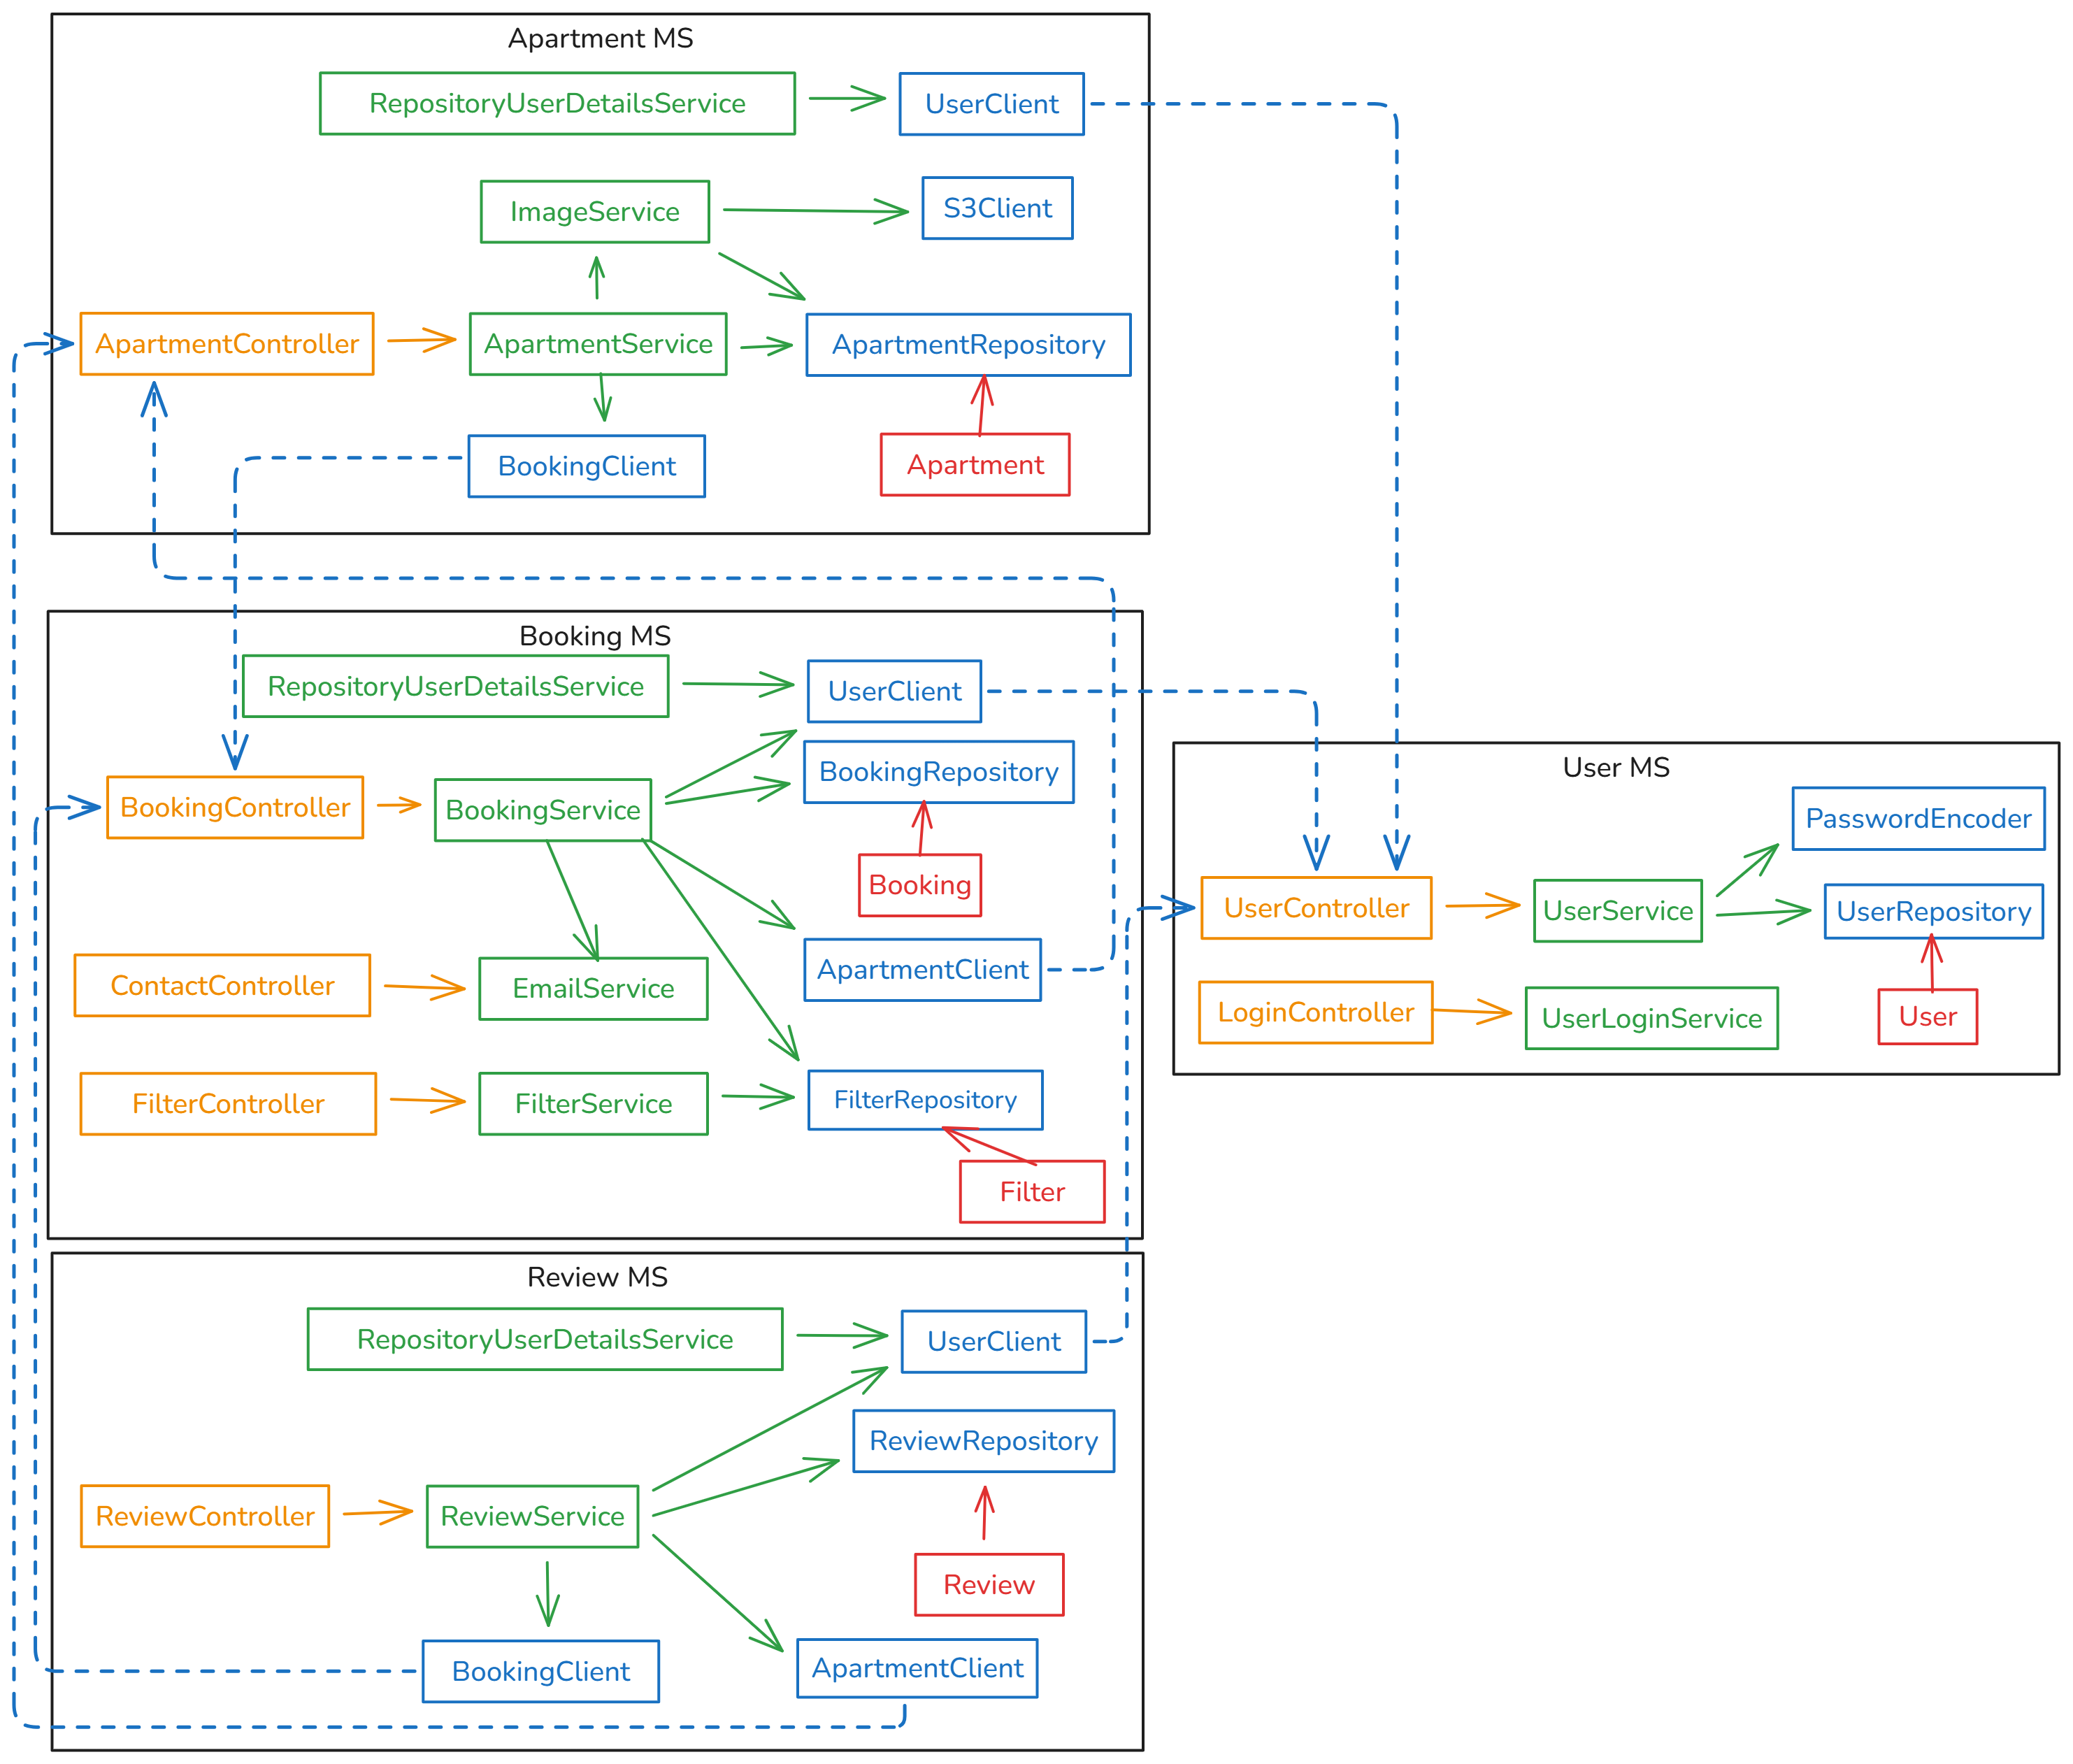
\includegraphics[width=1\textwidth, clip=true]{img/diagrama_server.png}
            \caption{Arquitectura en capas del servidor backend y comunicación entre microservicios.}
            \label{fig:arquitectura_servidor}
        \end{figure}

        Las responsabilidades de cada capa son las siguientes:
        \begin{itemize}
            \item \textbf{Controladores (\textit{Controllers}):} Capa externa que recibe las peticiones HTTP REST, valida los datos de entrada mediante el patrón DTO \cite[pp.~401--402]{fowler2002} y devuelve las respuestas con los códigos de estado adecuados, delegando siempre la lógica de negocio.
            \item \textbf{Servicios (\textit{Services}):} Núcleo del microservicio. Concentran toda la lógica de negocio, los cálculos algorítmicos (ej. motor de precios) y orquestan la comunicación síncrona con otros servicios mediante \textit{Feign Clients}.
            \item \textbf{Repositorios (\textit{Repositories}):} Abstraen el acceso a la base de datos implementando el patrón Repositorio \cite[pp.~322--327]{fowler2002} mediante Spring Data JPA, permitiendo realizar operaciones CRUD y consultas personalizadas sin necesidad de escribir sentencias SQL explícitas.
            \item \textbf{Entidades (\textit{Entities}):} Clases Java que representan el modelo de dominio y se mapean directamente a las tablas de MySQL mediante anotaciones de Hibernate.
        \end{itemize}

    \subsection{Arquitectura del Cliente}
        El cliente web construido con Angular sigue una arquitectura modular basada en componentes, diseñada para fomentar la reutilización de código y la reactividad de la interfaz de usuario (ver Figura \ref{fig:arquitectura_cliente}).

        \begin{figure}[H]
            \centering
            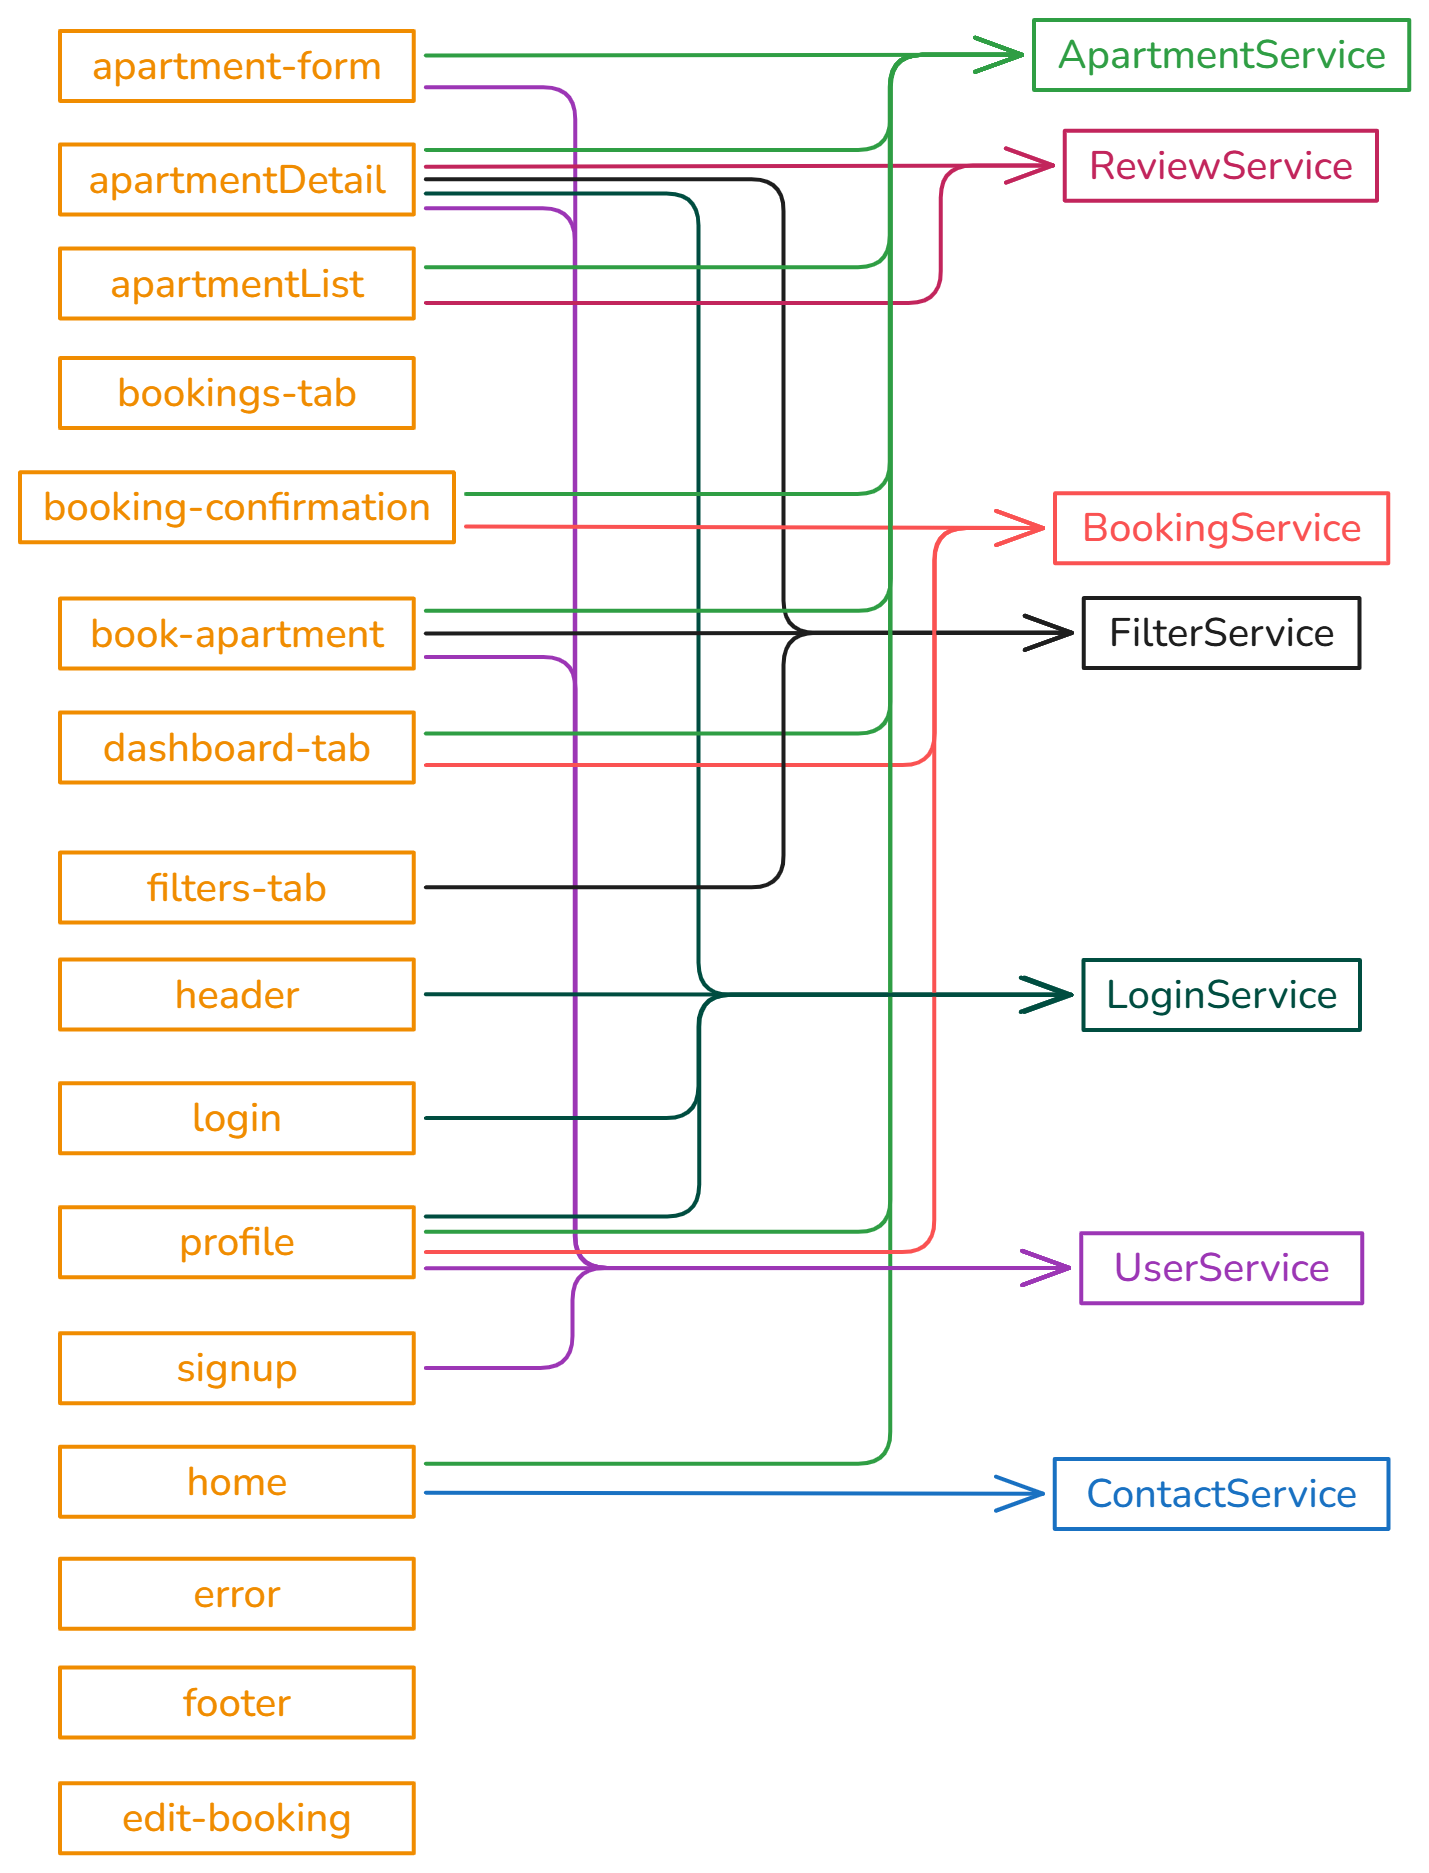
\includegraphics[width=0.6\textwidth, clip=true]{img/diagrama_cliente.png}
            \caption{Arquitectura del cliente Angular: Componentes, Servicios e Interceptores.}
            \label{fig:arquitectura_cliente}
        \end{figure}

        La separación por responsabilidades en el frontend se estructura en las siguientes capas:
        \begin{itemize}
            \item \textbf{Componentes (\textit{Components}):} Gestionan la vista (HTML/CSS) y la interacción del usuario. Se dividen en componentes de enrutamiento (páginas completas) y componentes presentacionales reutilizables (ej. \textit{Navbar} o \textit{Cards}).
            \item \textbf{Servicios (\textit{Services}):} Clases que aplican el patrón de inyección de dependencias \cite{fowler2004} para centralizar la lógica de negocio y aislar la comunicación externa mediante \texttt{HttpClient}. Destaca el uso de RxJS (\textit{BehaviorSubjects}) para gestionar estados globales, como la autenticación en el \textit{AuthService}.
            \item \textbf{Interceptores (\textit{Interceptors}):} \textit{Middleware} HTTP que procesa peticiones salientes y respuestas entrantes. Son fundamentales para aplicar lógicas globales de forma transparente, como ejecutar el refresco silencioso de tokens (\textit{Silent Refresh}) al detectar errores 401.
        \end{itemize}
\section{Implementación} 
\label{sec:implementacion}

En esta sección se describen los aspectos más relevantes del proceso de construcción del software, destacando decisiones de diseño significativas, desafíos técnicos encontrados y las soluciones algorítmicas adoptadas. Se focaliza la atención en aquellos componentes de la lógica de negocio que requirieron un mayor nivel de abstracción y estudio durante el desarrollo.

\subsection{Gestión de Autenticación y Seguridad con JWT}
Uno de los retos técnicos iniciales del sistema fue implementar un mecanismo de autenticación robusto, seguro y transparente para el usuario en una arquitectura distribuida sin estado (\textit{stateless}). La solución adoptada utiliza \textit{JSON Web Tokens} (JWT) combinada con una estrategia de \textit{Silent Refresh} gestionada por cookies de tipo \textit{HttpOnly}.

\subsubsection{Arquitectura de Seguridad y Flujo de Autenticación}
El sistema delega la responsabilidad de la seguridad de forma híbrida: el \textbf{User Service} actúa como servidor central de autorización, mientras que el resto de los microservicios actúan como recursos protegidos que validan la identidad de forma descentralizada.

Como se detalla en la Figura~\ref{fig:diagrama_jwt}, el flujo de autenticación garantiza que las credenciales sensibles y los tokens nunca persistan en el almacenamiento local del cliente (como \textit{LocalStorage}), utilizando el navegador como almacén seguro mediante cookies.

\begin{figure}[h]
    \centering
    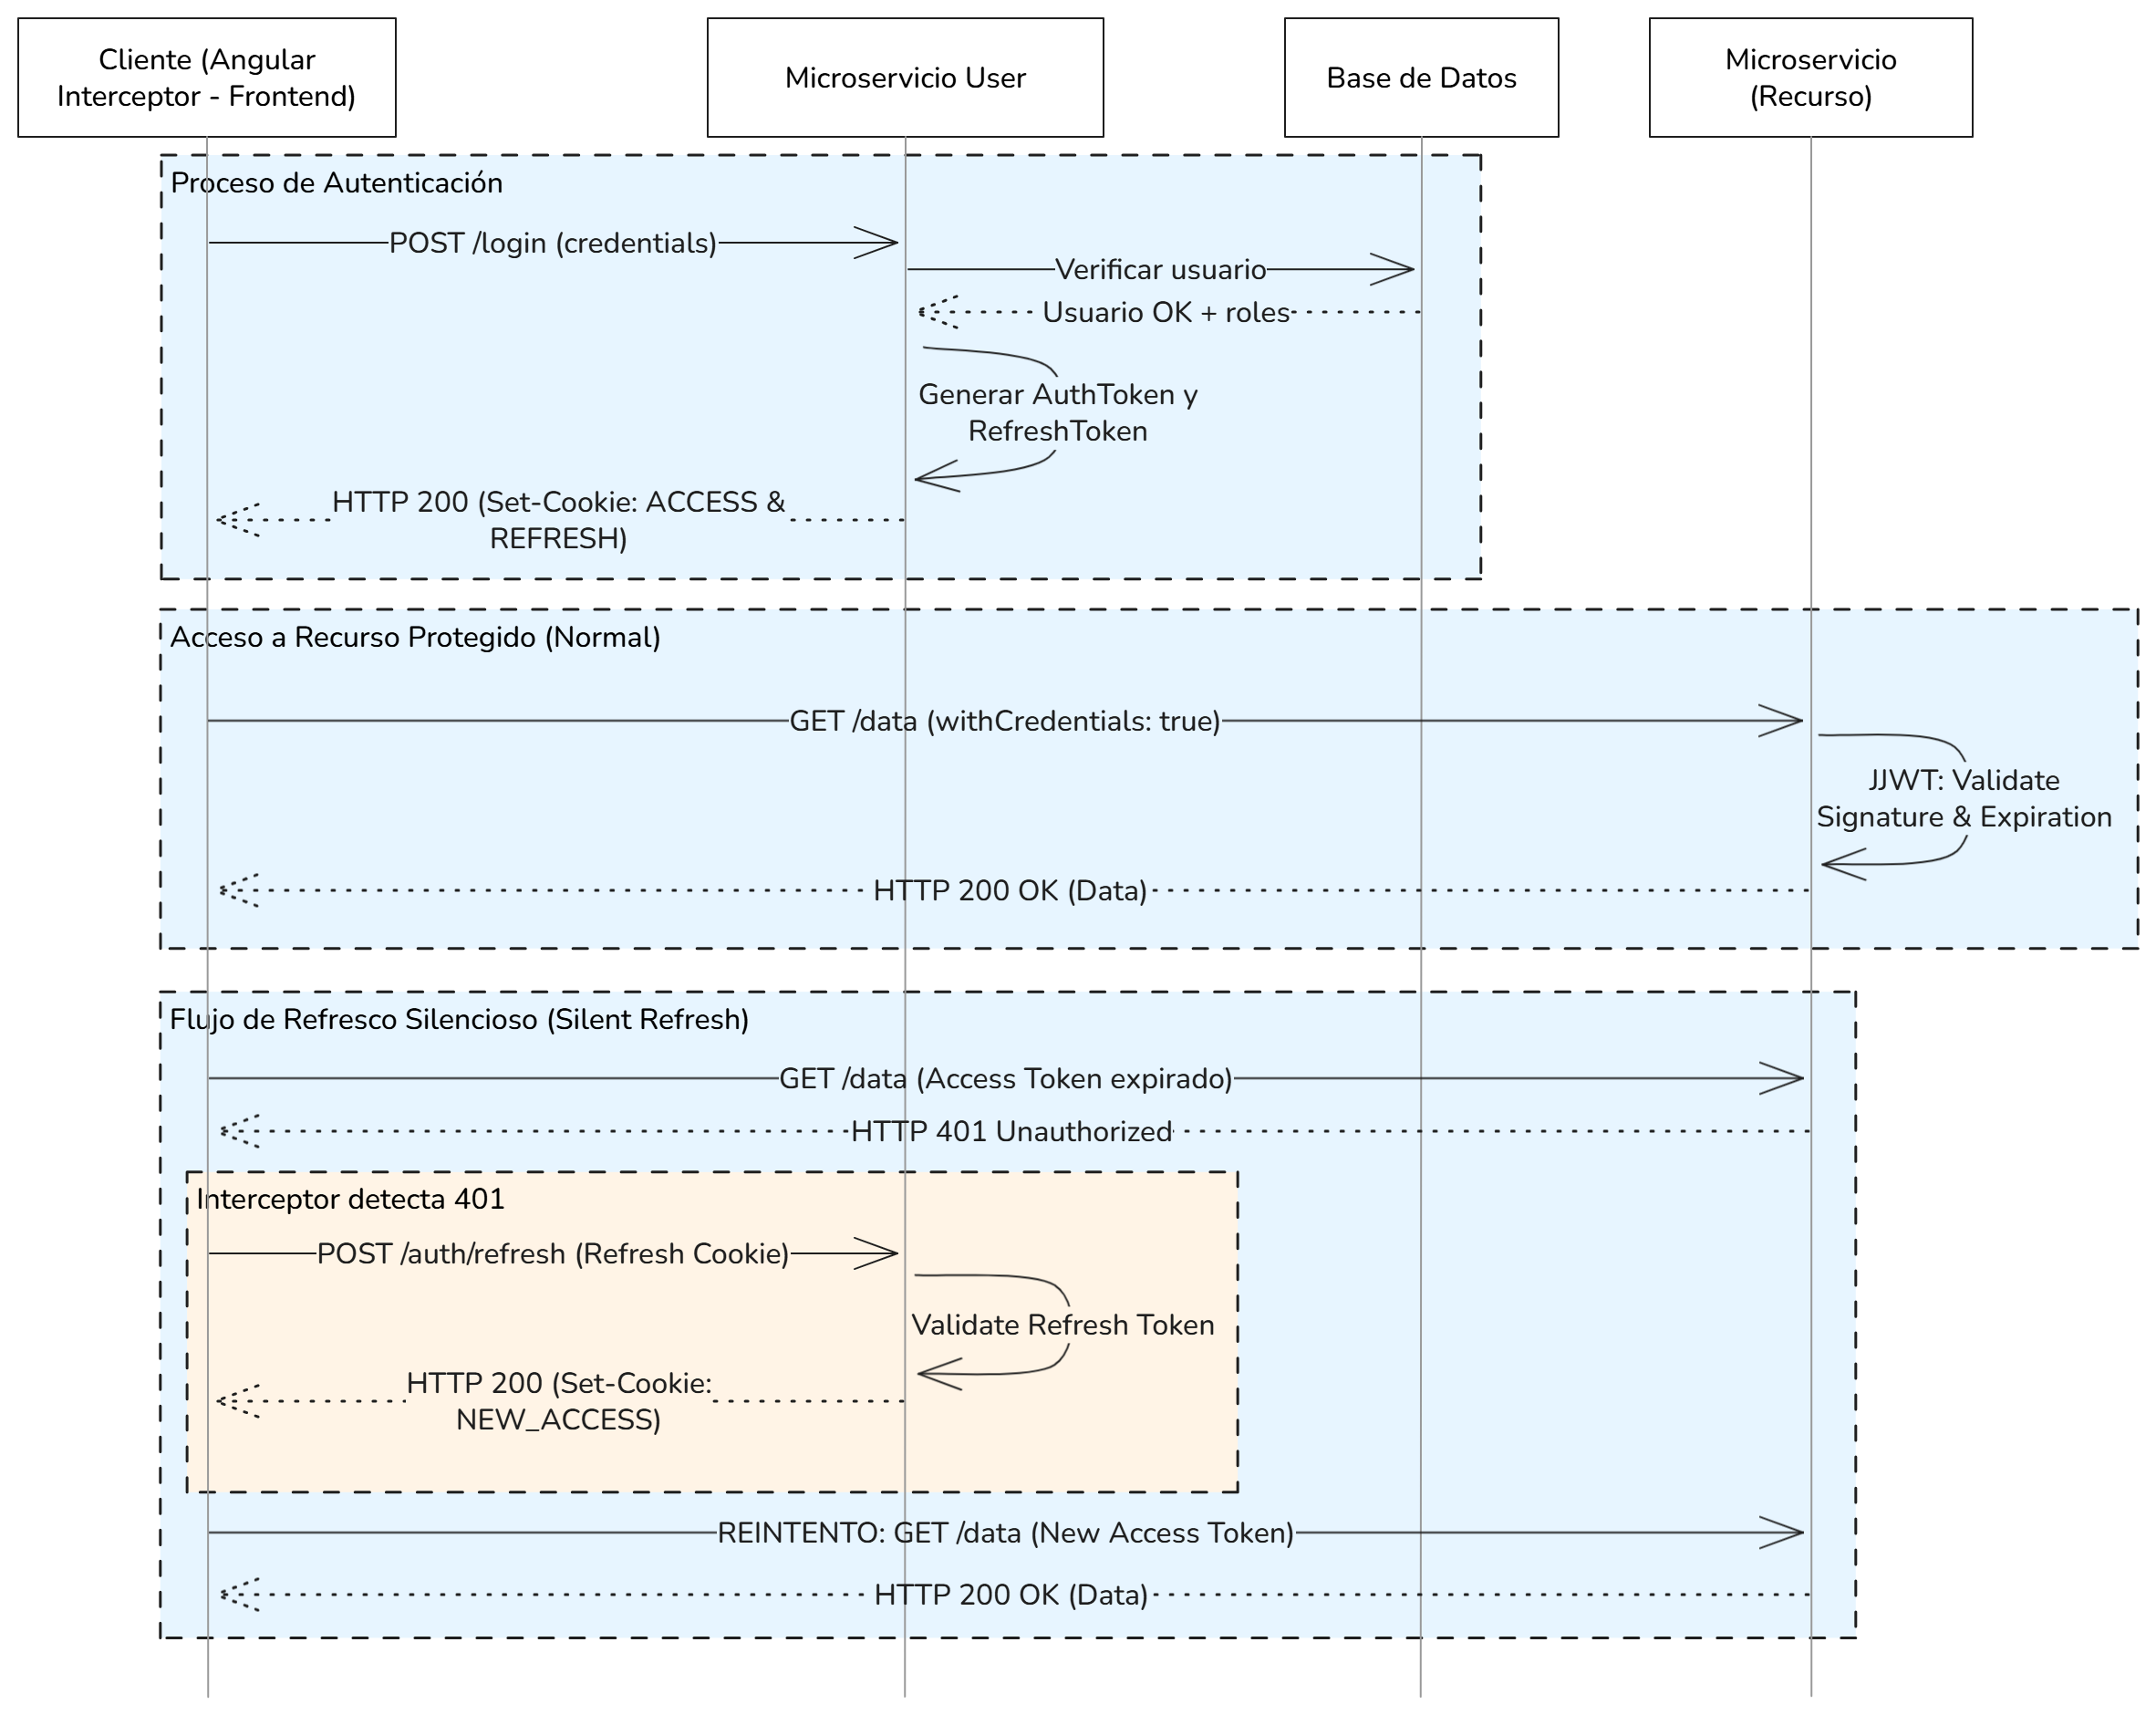
\includegraphics[width=0.9\textwidth]{img/diagrama_jwt.png}
    \caption{Diagrama de secuencia del proceso de autenticación, validación y refresco de tokens.}
    \label{fig:diagrama_jwt}
\end{figure}

\subsubsection{Generación de Tokens y Persistencia}
Tras la validación de credenciales mediante el \texttt{AuthenticationManager} de Spring Security, el sistema genera dos tipos de tokens con la librería JJWT (ver Código~\ref{lst:login_logic}):
\begin{itemize}
    \item \textbf{Auth Token}: Token de acceso de corta duración (5 minutos) firmado con el algoritmo HMAC-SHA512.
    \item \textbf{Refresh Token}: Token de larga duración (7 días) utilizado exclusivamente para solicitar nuevos tokens de acceso al servidor.
\end{itemize}

Ambos tokens se envían al cliente mediante el encabezado HTTP \texttt{Set-Cookie}, configurados estrictamente como \textit{HttpOnly} para mitigar los ataques de inyección de código (\textit{Cross-Site Scripting} o XSS), ya que impiden que el código JavaScript del cliente acceda a ellos.

\begin{lstlisting}[language=Java, caption={Lógica de login y creación de cookies en el User Service}, label={lst:login_logic}]
public ResponseEntity<AuthResponse> login(HttpServletResponse response, LoginRequest loginRequest) {
    Authentication auth = authenticationManager.authenticate(
        new UsernamePasswordAuthenticationToken(loginRequest.getUsername(), loginRequest.getPassword()));
    
    UserDetails user = (UserDetails) auth.getPrincipal();
    
    // Generacion de tokens y persistencia en cookies HttpOnly
    response.addCookie(buildTokenCookie(TokenType.ACCESS, jwtProvider.generateAccessToken(user)));
    response.addCookie(buildTokenCookie(TokenType.REFRESH, jwtProvider.generateRefreshToken(user)));

    return ResponseEntity.ok(new AuthResponse(Status.SUCCESS, "Auth successful"));
}
\end{lstlisting}

\subsubsection{Validación y Refresco Silencioso (Silent Refresh)}
Un aspecto diferencial de la implementación radica en la gestión de caducidad desde el \textbf{Interceptor HTTP de Angular}. Dado que el \textit{Auth Token} tiene una vida muy corta por motivos de seguridad, el interceptor monitoriza todas las respuestas del servidor. 

Si un microservicio devuelve un código de error \texttt{401 Unauthorized}, el interceptor de Angular captura el error, pausa temporalmente las peticiones salientes y lanza una petición asíncrona al \textit{endpoint} \texttt{/auth/refresh}. Si el \textit{Refresh Token} es válido, el servidor emite una nueva cookie y el interceptor reintenta la operación original automáticamente, sin que la experiencia del usuario se vea interrumpida.

\subsubsection{Seguridad de las Claves}
Para garantizar la integridad del sistema en diferentes entornos, la clave secreta JWT no se encuentra codificada en el código fuente (\textit{hardcoded}). Se gestiona mediante variables de entorno inyectadas en tiempo de ejecución, lo que permite rotar las claves en producción sin necesidad de recompilar los artefactos.

\subsection{Motor de Precios Dinámicos}
La funcionalidad troncal y más compleja de la lógica de negocio ha sido el \textbf{motor de precios dinámico}, que permite ajustar el coste por noche de los alojamientos en tiempo real basándose en reglas contextuales.

\subsubsection{Concepto y Arquitectura}
Un filtro de precio es una regla que especifica el tipo de ajuste (incremento o descuento), el porcentaje de ajuste y las condiciones de aplicación.

\subsubsection{Diseño Flexible de la Entidad Filter}
El aspecto más destacable del sistema es el diseño de la entidad \texttt{Filter}, que utiliza un patrón de configuración flexible mediante campos opcionales que se combinan para representar diferentes tipos de reglas (\ref{lst:filter}):

\begin{lstlisting}[ caption={Entidad Filter para sistema dinámico de precios}, label={lst:filter}]
@Entity
public class Filter {
    private Long id;
    private String name;
    private String description;
    private Boolean activated;
    private Boolean increment;        // true = incremento, false = descuento
    private BigDecimal value;         // Porcentaje de ajuste
    
    // Configuracion temporal
    private DateType dateType;        // DATE_RANGE | EVERY_DAY | WEEK_DAYS | DATE_RANGE_WEEK_DAYS
    private LocalDate startDate;      // Requerido si dateType incluye rango
    private LocalDate endDate;        // Requerido si dateType incluye rango
    private String weekDays;          // Requerido si dateType incluye dias (valores: 1-7)
    
    // Condiciones adicionales
    private ConditionType conditionType;  // LAST_MINUTE | LONG_STAY | NONE
    private Integer anticipationHours;    // Requerido si conditionType = LAST_MINUTE
    private Integer minDays;              // Requerido si conditionType = LONG_STAY
}
\end{lstlisting}












La clave del diseño está en que los campos obligatorios dependen de los valores de los enums. El sistema utiliza dos enums:

\textbf{DateType} determina cuándo aplica el filtro temporalmente:
\begin{itemize}
\item \texttt{DATE\_RANGE}: Aplica en un rango específico de fechas (requiere \texttt{startDate} y \texttt{endDate})
\item \texttt{WEEK\_DAYS}: Aplica solo ciertos días de la semana (requiere \texttt{weekDays})
\item \texttt{EVERY\_DAY}: Aplica todos los días sin restricción
\item \texttt{DATE\_RANGE\_WEEK\_DAYS}: Aplica ciertos días dentro de un rango

(requiere \texttt{startDate}, \texttt{endDate} y \texttt{weekDays})
\end{itemize}

\textbf{ConditionType} añade condiciones adicionales sobre la reserva:
\begin{itemize}
\item \texttt{LAST\_MINUTE}: Aplica para reservas con poca antelación

(requiere \texttt{anticipationHours})
\item \texttt{LONG\_STAY}: Aplica solo para estancias de duración mínima (requiere \texttt{minDays})
\item \texttt{NONE}: Sin condición adicional
\end{itemize}

Este enfoque proporciona máxima flexibilidad porque permite combinaciones complejas (por ejemplo, descuento solo en verano y solo para estancias largas), utiliza validación condicional de campos según los enums seleccionados, presenta una interfaz adaptativa que muestra/oculta campos dinámicamente y evita la proliferación de entidades.

Con esta estructura, el sistema puede representar cualquier combinación lógica de restricciones temporales y condiciones de reserva, cubriendo escenarios desde descuentos generales permanentes hasta combinaciones complejas como estancias largas en fines de semana de verano. Esto representa múltiples tipos diferentes de reglas de negocio sin necesidad de crear múltiples entidades o tablas.

Esta arquitectura de \textbf{configuración sobre código} es un ejemplo de aplicación del principio de diseño ``Open/Closed'': el sistema está abierto a extensión (se pueden crear infinitas combinaciones de reglas) pero cerrado a modificación (no hay que cambiar código para añadir nuevos tipos de reglas).

\subsubsection{Consulta de Filtros Aplicables}
El sistema expone un endpoint que permite consultar qué filtros aplicarían a unas fechas específicas antes de realizar la reserva:

\texttt{GET \\ /api/v1/filters/applicable?checkIn=2026-07-16\&checkOut=2026-07-18}

La respuesta organiza los filtros por fecha, mostrando para cada noche de la estancia qué ajustes de precio aplican:
 \begin{lstlisting}
    {
        "checkInDate": "2026-07-16",
        "checkOutDate": "2026-07-18",
        "totalNights": 2,
        "filtersByDate": {
            "2026-07-16": [],
            "2026-07-17": [
                {
                    "id": 1,
                    "name": "Weekend Premium",
                    "description": "Price increase for Friday, Saturday and Sunday nights",
                    "activated": true,
                    "increment": true,
                    "value": 20.00,
                    "dateType": "WEEK_DAYS",
                    "startDate": null,
                    "endDate": null,
                    "weekDays": "5,6,7",
                    "conditionType": "NONE",
                    "anticipationHours": null,
                    "minDays": null,
                    "createdAt": null,
                    "updatedAt": null
                }
            ]
        }
    }
 \end{lstlisting}
 
Esta estructura permite al frontend mostrar una previsualización del precio desglosado noche por noche, dando transparencia al usuario sobre cómo se ha calculado el precio total.


\subsubsection{Cálculo del Precio Final}
Cuando se crea una reserva, el Booking Service obtiene el precio base del apartamento, consulta los filtros aplicables y, para cada noche, aplica secuencialmente cada filtro activo sobre el precio base, acumulando el precio ajustado al total.

Por ejemplo, si un apartamento cuesta \EUR{100}/noche y el usuario reserva un viernes con 20\% de incremento por fin de semana más 10\% de descuento por reserva anticipada, el precio final de esa noche sería \EUR{110} (\EUR{100} + \EUR{20} - \EUR{10}).

\subsubsection{Ventajas del Sistema}
Este diseño proporciona:
\begin{itemize}
\item \textbf{Flexibilidad total}: Los administradores pueden crear cualquier combinación de reglas sin modificar código ni base de datos
\item \textbf{Transparencia}: Los usuarios ven exactamente qué ajustes se están aplicando y por qué
\item \textbf{Competitividad}: Permite implementar estrategias de pricing dinámico similares al \textit{yield management}\footnote{Yield management: estrategia de gestión de ingresos que ajusta precios según demanda y disponibilidad \cite{kimes1989}.} utilizado por aerolíneas y hoteles
\item \textbf{Automatización}: Los precios se ajustan automáticamente según las reglas configuradas, sin intervención manual
\item \textbf{Experimentación}: Fácil probar diferentes estrategias activando/desactivando filtros y midiendo su impacto
\item \textbf{Escalabilidad}: El sistema puede manejar decenas de filtros simultáneos sin degradación de rendimiento
\end{itemize}
Los administradores gestionan los filtros desde un panel dedicado en el frontend, donde pueden crear, editar, activar/desactivar y eliminar reglas mediante formularios intuitivos, sin necesidad de conocimientos técnicos ni programación.

\subsection{Envío de Emails con JavaMailSender}
El Booking Service implementa funcionalidad de notificaciones por email usando Spring Mail.

\subsubsection{Configuración del Servidor SMTP}
La configuración utiliza Gmail SMTP\footnote{SMTP: Simple Mail Transfer Protocol, protocolo estándar para envío de correo electrónico} con autenticación de dos factores mediante contraseña de aplicación. Las credenciales se externalizan mediante variables de entorno para diferentes entornos, permitiendo flexibilidad entre desarrollo y producción.

\subsubsection{Servicio de Email}
El \texttt{EmailService} encapsula la lógica de envío utilizando \texttt{JavaMailSender} y \texttt{MimeMessage} para permitir HTML y archivos adjuntos, con soporte UTF-8 para caracteres internacionales. El servicio implementa manejo de errores silencioso: un fallo en el email no impide crear la reserva.

El servicio proporciona múltiples tipos de notificaciones: confirmación al crear una reserva, actualización al modificar, cancelación y recordatorio programado antes del check-in.


\section{Control de calidad} 
\label{sec:control_calidad}

La estrategia de pruebas del proyecto abarca múltiples niveles tanto en el backend como en el frontend, garantizando la calidad, fiabilidad y correcto funcionamiento del sistema mediante pruebas automatizadas que cubren desde la validación de componentes individuales hasta la verificación de flujos completos de usuario.

\subsection{Estrategia de Testing}
El proyecto sigue la pirámide de testing clásica \cite{fowler2012}, distribuyendo las pruebas en tres niveles:
\begin{itemize}
\item \textbf{Base - Tests Unitarios}: Mayor cantidad de pruebas, ejecución rápida, validan componentes aislados
\item \textbf{Medio - Tests de Integración}: Cantidad moderada, verifican interacciones entre componentes y con infraestructura real
\item \textbf{Cima - Tests End-to-End}: Menor cantidad, costosos pero verifican flujos completos de usuario
\end{itemize}

Esta distribución permite detectar fallos rápidamente en las fases tempranas del desarrollo mientras se garantiza que el sistema funciona correctamente como un todo.

\subsection{Pruebas del Backend}
Los microservicios del backend han sido sometidos a tres tipos de pruebas automatizadas para garantizar la corrección de la lógica de negocio, la persistencia de datos y la comunicación entre servicios.

\subsubsection{Tipos de Pruebas Implementadas}
\begin{itemize}
    \item \textbf{Tests Unitarios:} Validan la lógica de negocio de forma aislada utilizando Mockito para simular dependencias (repositorios y clientes Feign), sin requerir el levantamiento de bases de datos o servicios externos.
    \item \textbf{Tests de Integración:} Verifican el comportamiento del sistema con bases de datos reales mediante contenedores MySQL efímeros (Testcontainers). Validan el mapeo de entidades JPA, las consultas personalizadas y la integridad transaccional.
    \item \textbf{Tests End-to-End (E2E):} Validan flujos completos a través del \textit{API Gateway} realizando peticiones HTTP reales con REST Assured. Verifican la autenticación JWT y la correcta comunicación cruzada entre los distintos microservicios en ejecución.
\end{itemize}

\subsubsection{Cobertura de Código por Microservicio}
La cobertura se mide mediante JaCoCo, que genera reportes HTML detallados tras ejecutar \texttt{mvn test}. Las Figuras \ref{fig:jacoco_apartment}, \ref{fig:jacoco_user}, \ref{fig:jacoco_booking} y \ref{fig:jacoco_review} muestran los reportes.

\begin{figure}[H]
\centering
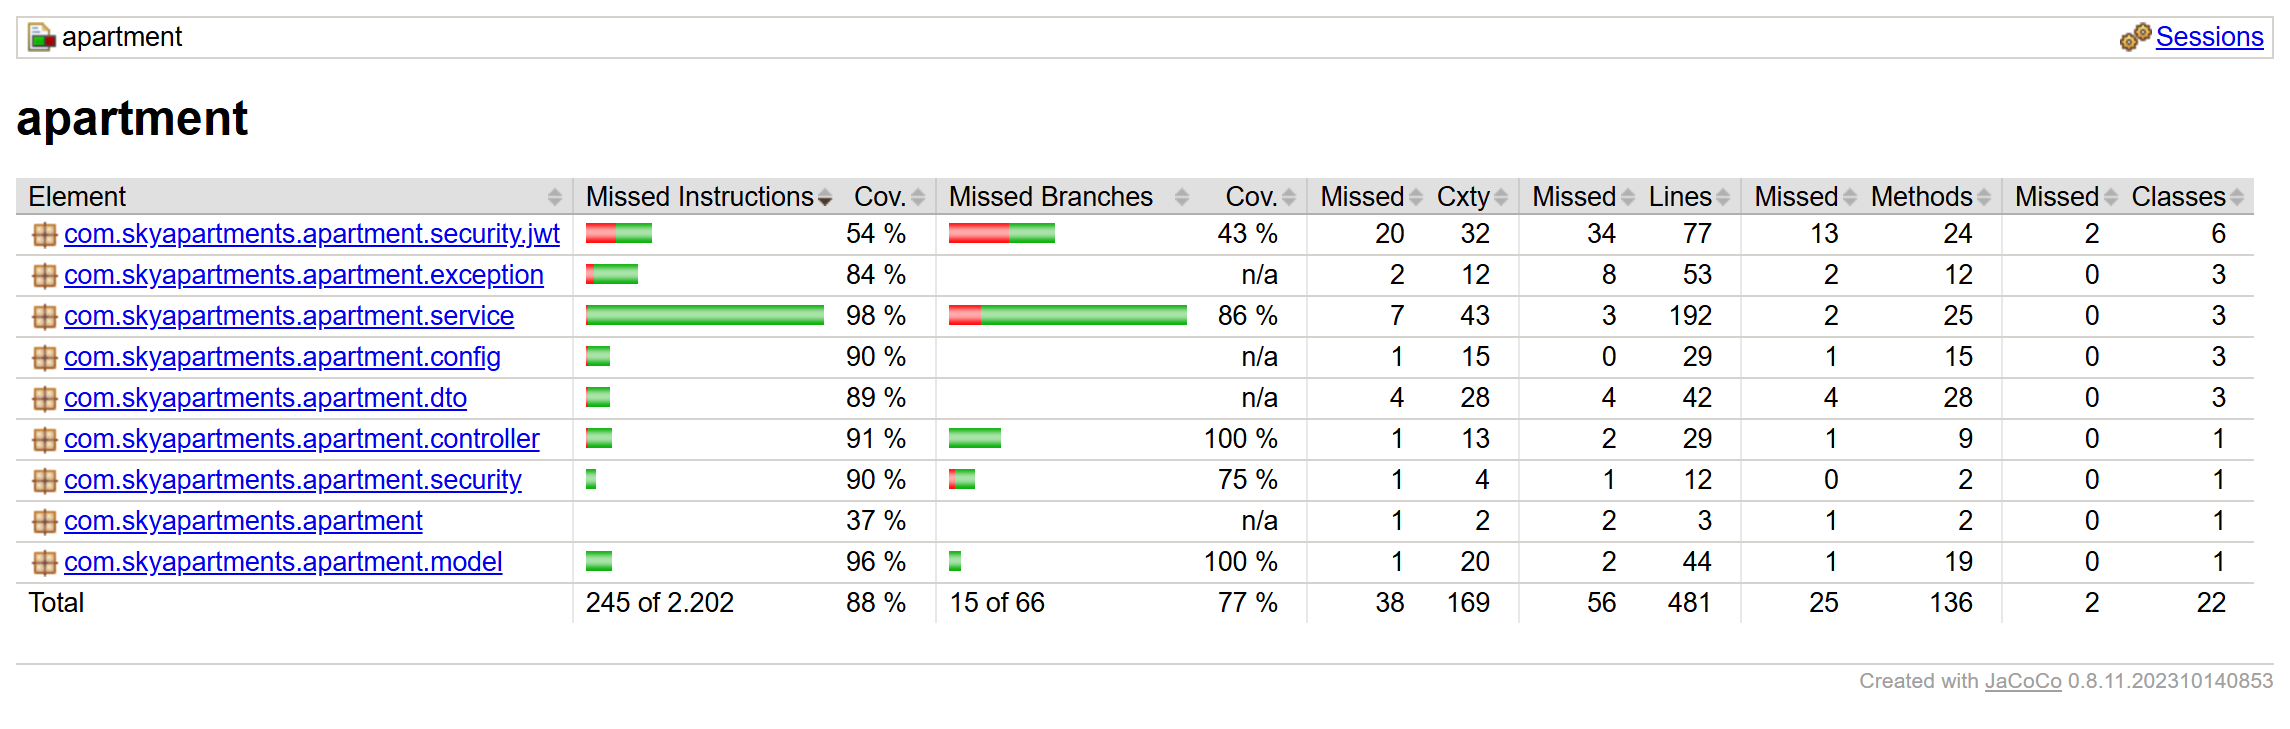
\includegraphics[width=0.9\textwidth]{img/jacoco_apartment.png}
\caption{Reporte de cobertura JaCoCo - Apartment Service}
\label{fig:jacoco_apartment}
\end{figure}

\begin{figure}[H]
\centering
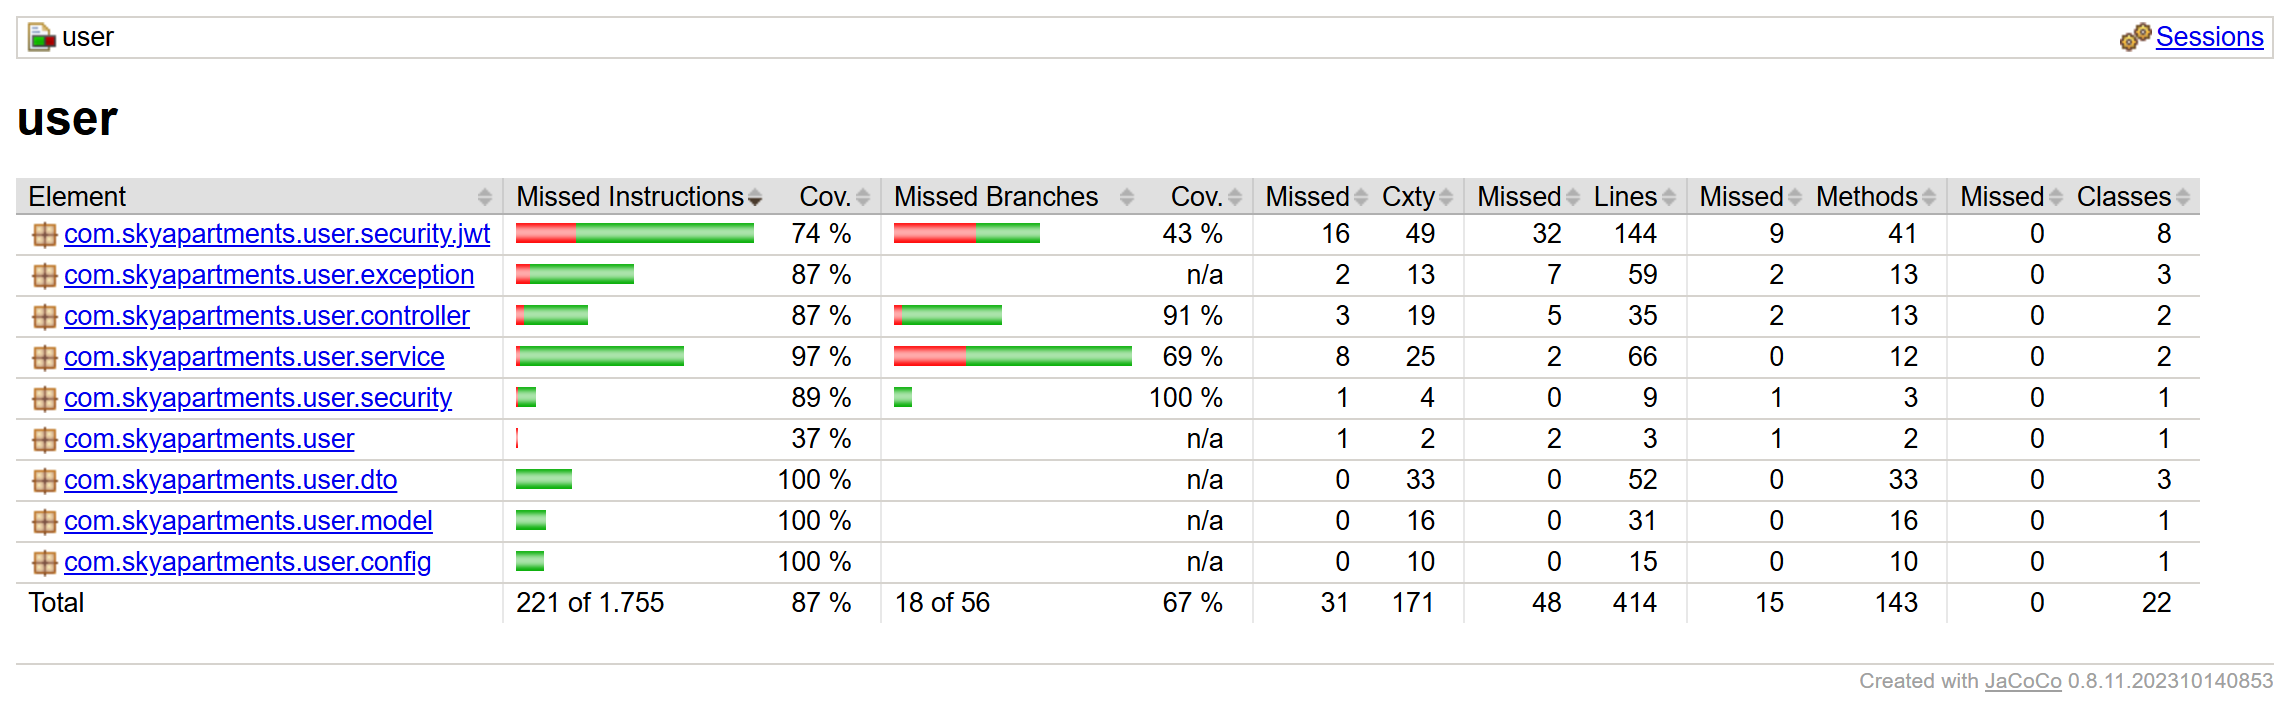
\includegraphics[width=0.9\textwidth]{img/jacoco_user.png}
\caption{Reporte de cobertura JaCoCo - User Service}
\label{fig:jacoco_user}
\end{figure}

\begin{figure}[H]
\centering
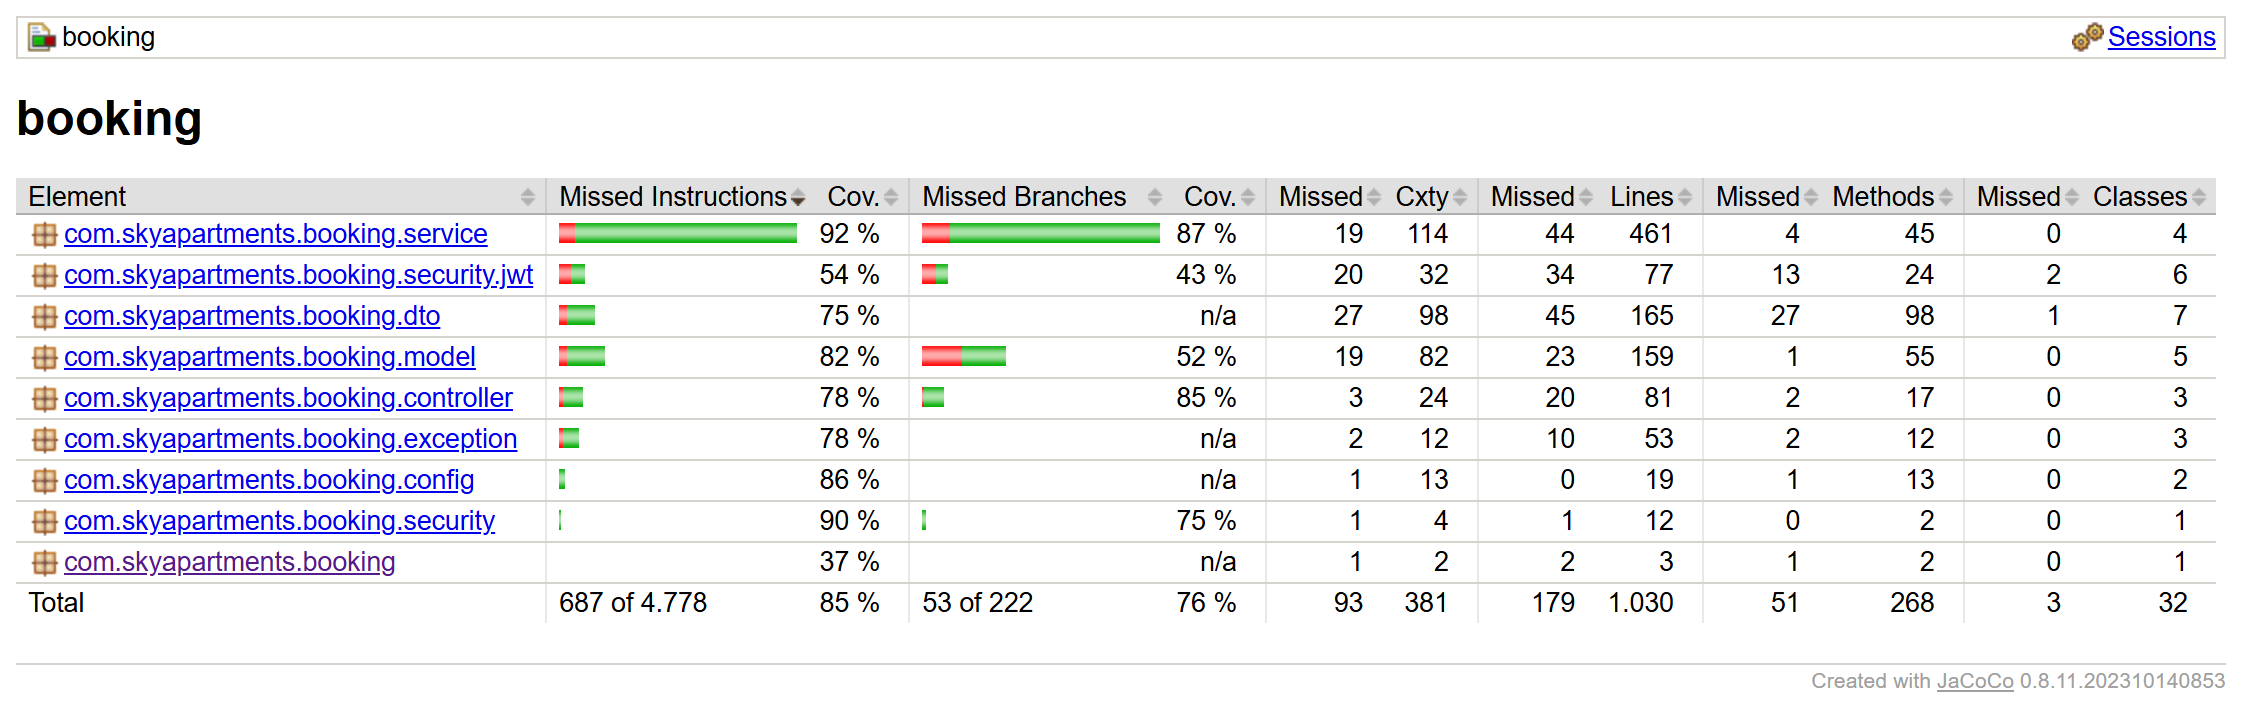
\includegraphics[width=0.9\textwidth]{img/jacoco_booking.png}
\caption{Reporte de cobertura JaCoCo - Booking Service}
\label{fig:jacoco_booking}
\end{figure}

\begin{figure}[H]
\centering
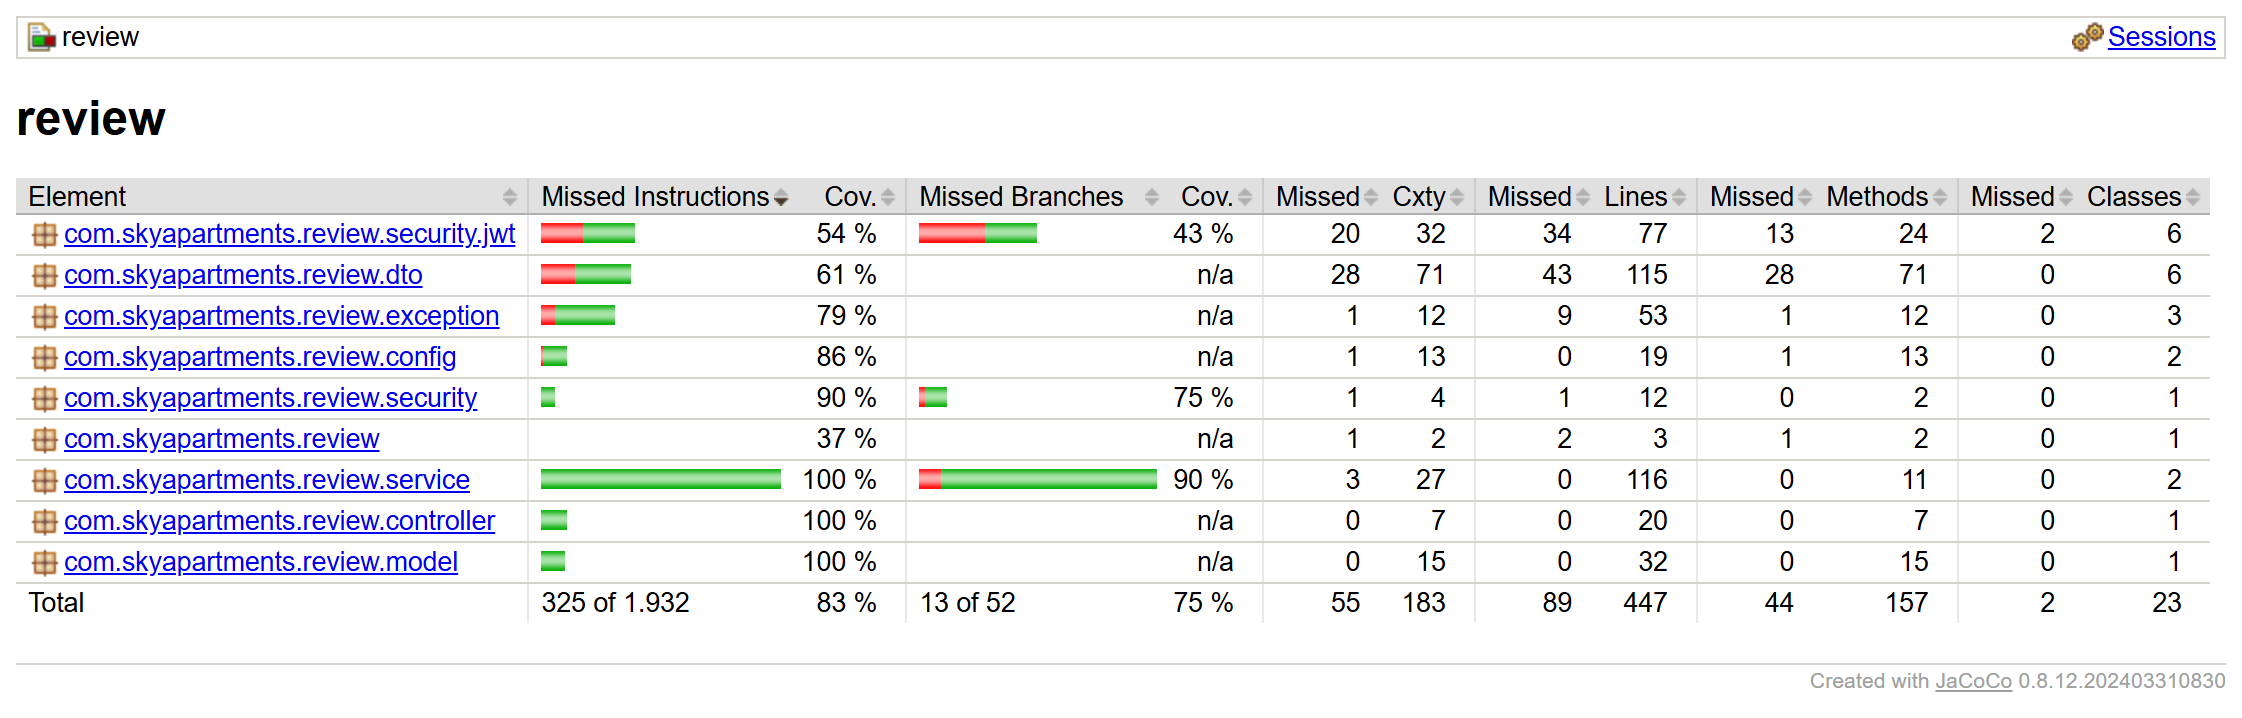
\includegraphics[width=0.9\textwidth]{img/jacoco_review.png}
\caption{Reporte de cobertura JaCoCo - Review Service}
\label{fig:jacoco_review}
\end{figure}

Los cuatro microservicios principales superan el umbral mínimo del 80\% de cobertura de líneas. Las capas de servicio y controladores alcanzan coberturas superiores al 75\% en todos los casos. Las entidades del modelo muestran coberturas del 82-100\% debido a que los tests de integración ejercitan exhaustivamente el mapeo JPA.

\subsection{Pruebas del frontend}
El frontend Angular ha sido testado en tres niveles: tests unitarios, tests de integración y tests end-to-end, garantizando tanto la corrección de componentes individuales como la validación de flujos completos de usuario.

\subsubsection{Tipos de Pruebas Implementadas}
\begin{itemize}
    \item \textbf{Tests Unitarios:} Validan la lógica de componentes aislados mediante un DOM virtual y servicios simulados (\textit{mocks}), empleando Jasmine como \textit{framework} y Karma como \textit{test runner}.
    \item \textbf{Tests de Integración:} Verifican la interacción entre componentes mediante \texttt{TestBed} de Angular, realizando peticiones HTTP reales al \textit{API Gateway} para validar el mapeo de objetos JSON y el manejo de errores.
    \item \textbf{Tests End-to-End (E2E):} Simulan flujos de usuario en navegadores reales mediante Playwright (clics, navegación, escritura). Requieren el backend en ejecución para certificar la integración completa entre el frontend y la base de datos.
\end{itemize}
\subsubsection{Cobertura de Tests Unitarios e Integración}
La cobertura del frontend se genera mediante Karma + Istanbul. El proyecto alcanza una cobertura del 90.94\% en líneas de código, 91.22\% en funciones, 82.34\% en ramas y 90.76\% en sentencias.

La Figura \ref{fig:frontend_coverage} muestra el reporte visual de cobertura generado por Istanbul, que permite identificar archivos con baja cobertura, líneas específicas no cubiertas, ramas condicionales no ejercitadas y funciones no invocadas durante los tests.

\begin{figure}[!h]
\centering
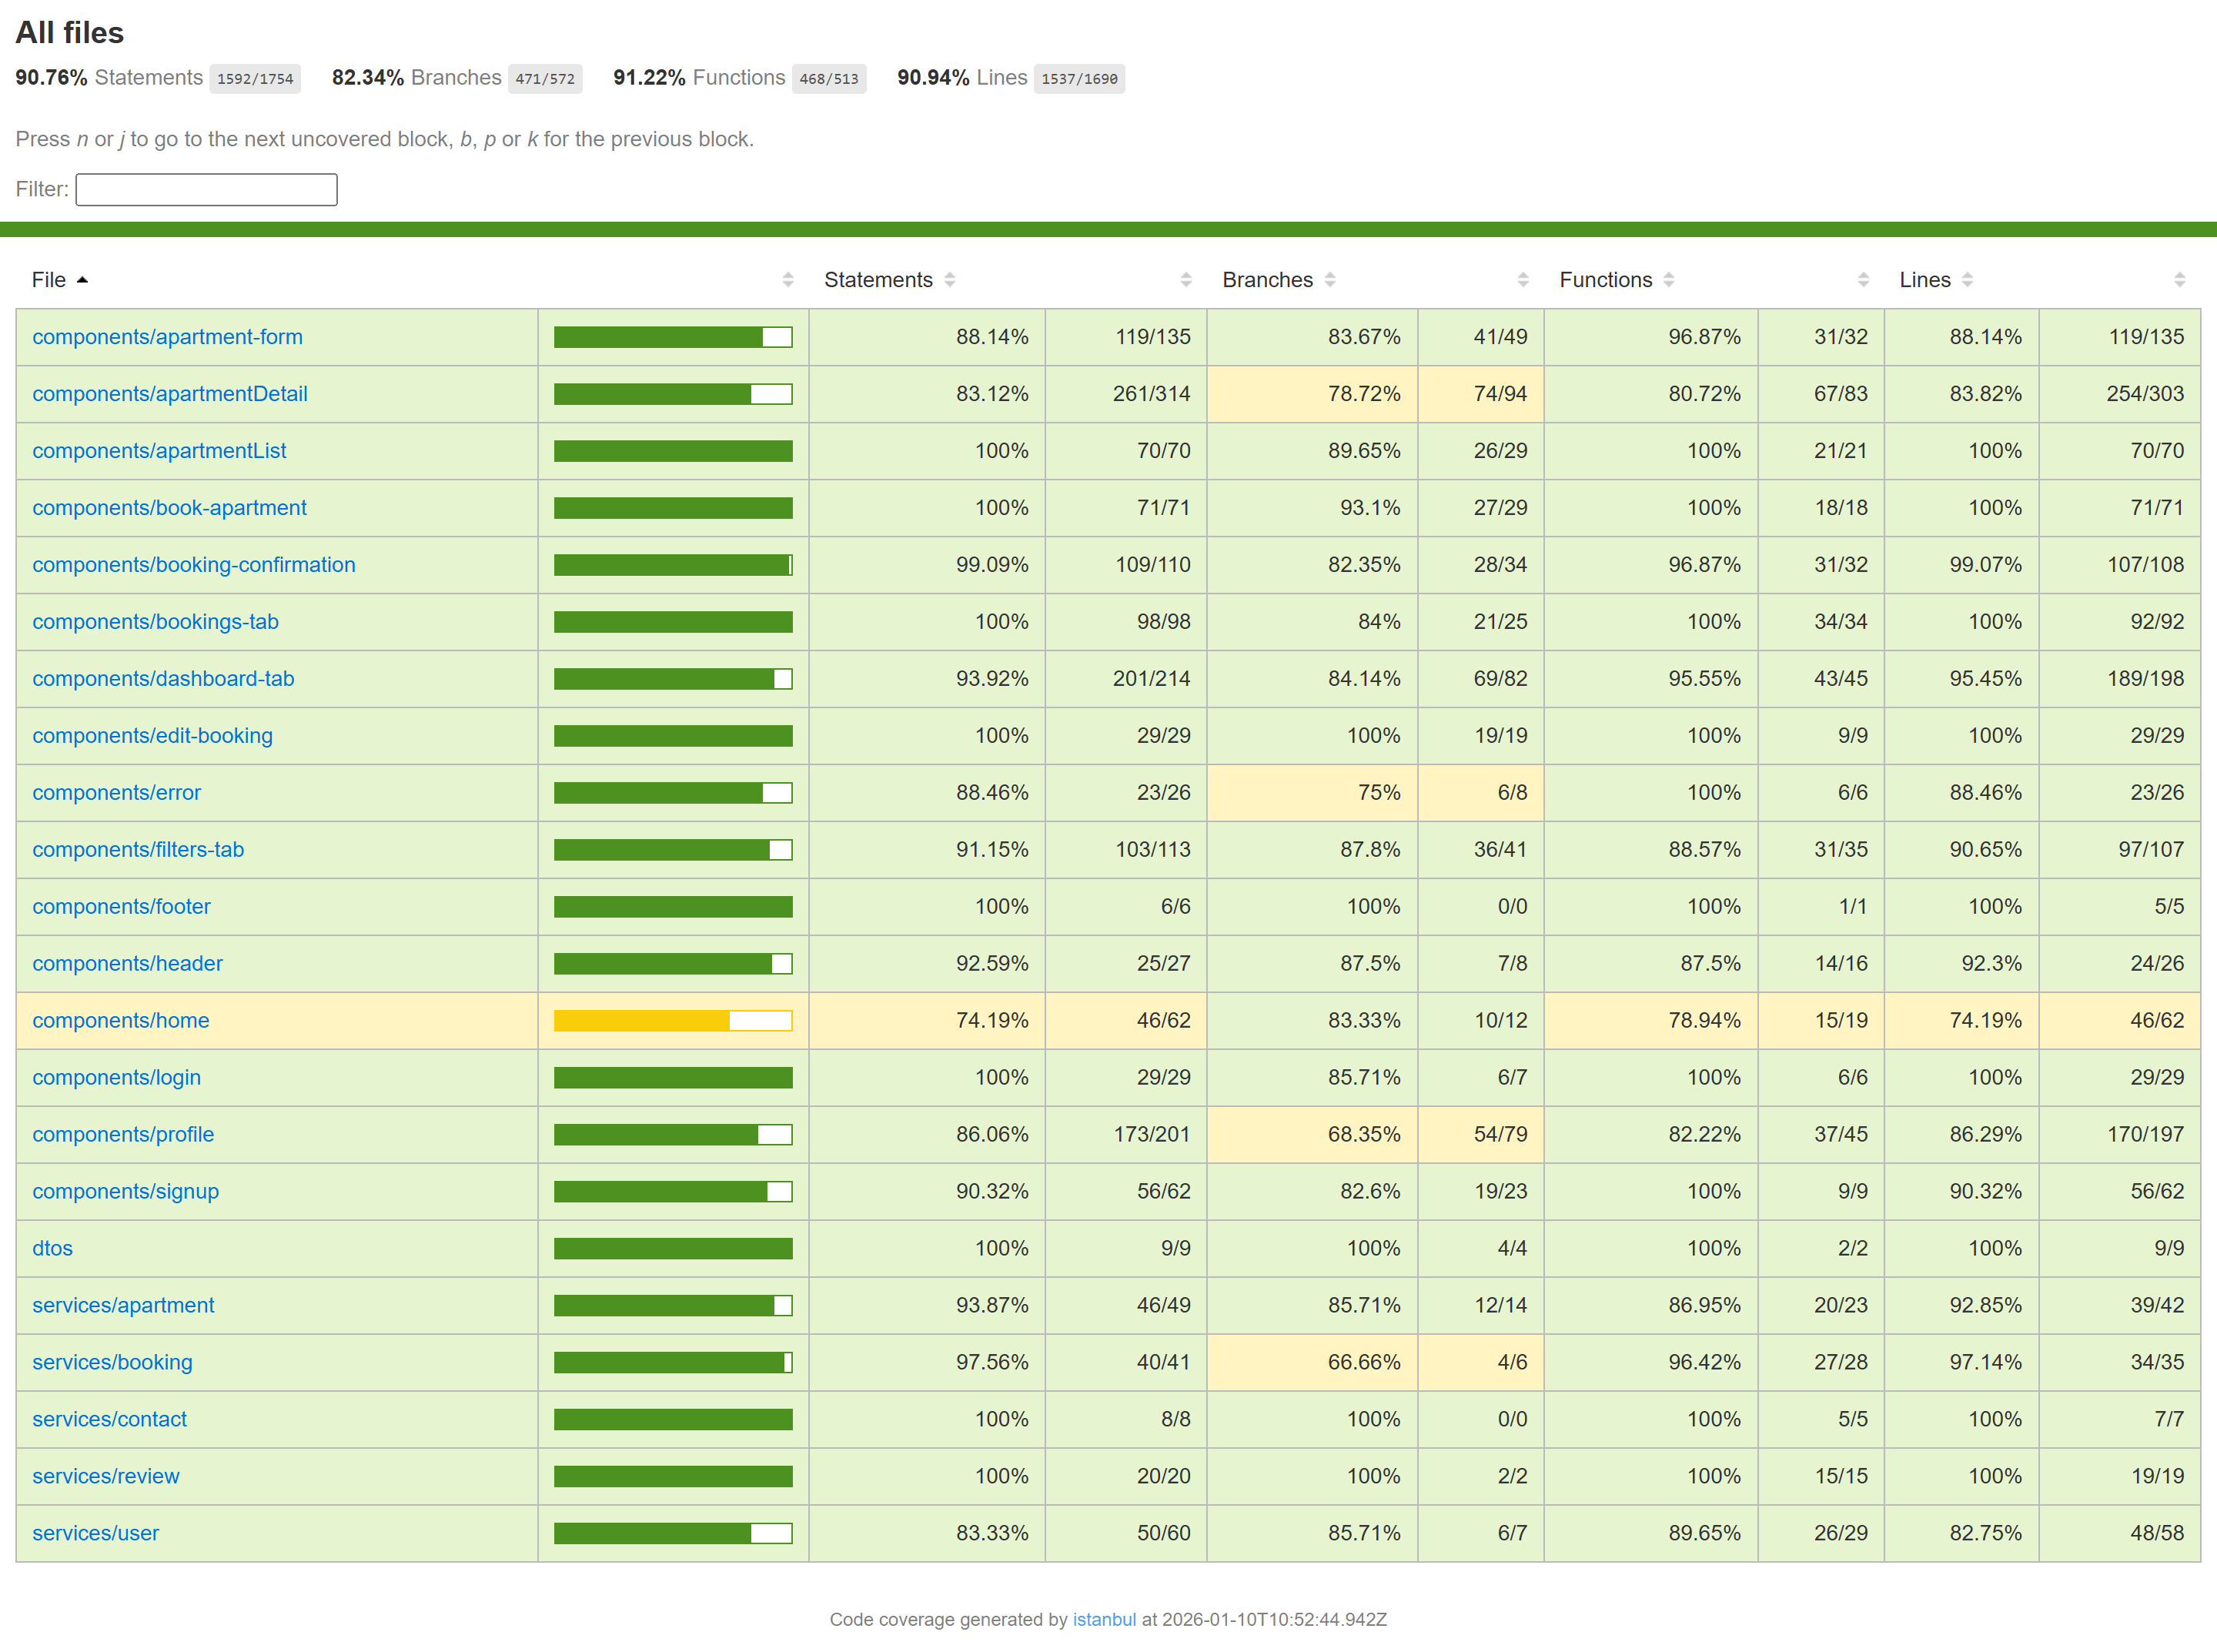
\includegraphics[width=0.95\textwidth]{img/informe_front.png}
\caption{Reporte de cobertura del frontend - Tests unitarios e integración}
\label{fig:frontend_coverage}
\end{figure}

\subsubsection{Tests End-to-End con Playwright}
Los tests E2E validan flujos completos incluyendo autenticación de usuarios, navegación y filtrado de apartamentos, creación y gestión de reservas, escritura de reseñas e interacciones que involucran múltiples microservicios.

\subsection{Análisis de Resultados}
El proyecto alcanza niveles de cobertura satisfactorios: 80-88\% de cobertura de líneas en el backend según el microservicio, 90.94\% en el frontend, y una cobertura global estimada de aproximadamente 85\% considerando todo el código del proyecto. Estos valores superan el umbral mínimo del 75-80\% considerado estándar en la industria, garantizando que la mayor parte del código está cubierta por tests automatizados que detectarían regresiones en futuras modificaciones.
\section{Despliegue}
\label{sec:despliegue}

En esta sección se describe el empaquetado mediante contenedores, la distribución de 
artefactos y el despliegue en la nube (AWS).

\subsection{Empaquetado y Distribución}

Para facilitar la distribución, se utiliza un \textit{Dockerfile multi-etapa} que genera 
\textbf{una única imagen Docker} agrupando el cliente (Angular) y el servidor (microservicios 
Spring Boot, Eureka y \textit{API Gateway}). Esta estrategia, adoptada por las limitaciones de recursos 
del entorno académico, garantiza un versionado coherente y optimiza el consumo de memoria de 
la instancia EC2. El proceso compila el backend (Maven/JDK 17) y el frontend (Node.js) de 
forma independiente, fusionando los binarios resultantes en una imagen final ligera 
(Alpine + JRE 17) orquestada por un \textit{script} de arranque secuencial.

Para gestionar el entorno completo se utiliza \textbf{Docker Compose}, inyectando la 
configuración sensible dinámicamente mediante un archivo \texttt{.env}. Este archivo define 
la infraestructura como código (\textit{Infrastructure as Code}), creando la red virtual, 
los volúmenes persistentes y coordinando:
\begin{itemize}
    \item El contenedor principal de la aplicación Sky Apartments.
    \item Un único motor \textbf{MySQL 8.0} con cuatro esquemas de base de datos independientes 
    (uno por microservicio: \texttt{usersdb}, \texttt{apartmentsdb}, \texttt{bookingsdb} y 
    \texttt{reviewsdb}), preservando el aislamiento lógico de datos que exige el patrón 
    \textit{Database per Service}~\cite[Cap.~5]{richardson2018}.
    \item MinIO (almacenamiento de objetos) y Jaeger (trazabilidad distribuida).
\end{itemize}

La imagen final y el manifiesto de infraestructura se distribuyen de forma pública a través 
de \textbf{DockerHub}, estando disponibles en la siguiente URL: \\
\url{https://hub.docker.com/r/eloydsdlh/apartments-app}

\subsection{Despliegue en la Nube (AWS)}

La aplicación está desplegada en producción sobre \textbf{Amazon Web Services (AWS)}, 
utilizando el servicio \textbf{Amazon EC2}. La Figura~\ref{fig:despliegue_aws} ilustra 
la topología de red del entorno de producción.

\begin{figure}[!h]
\centering
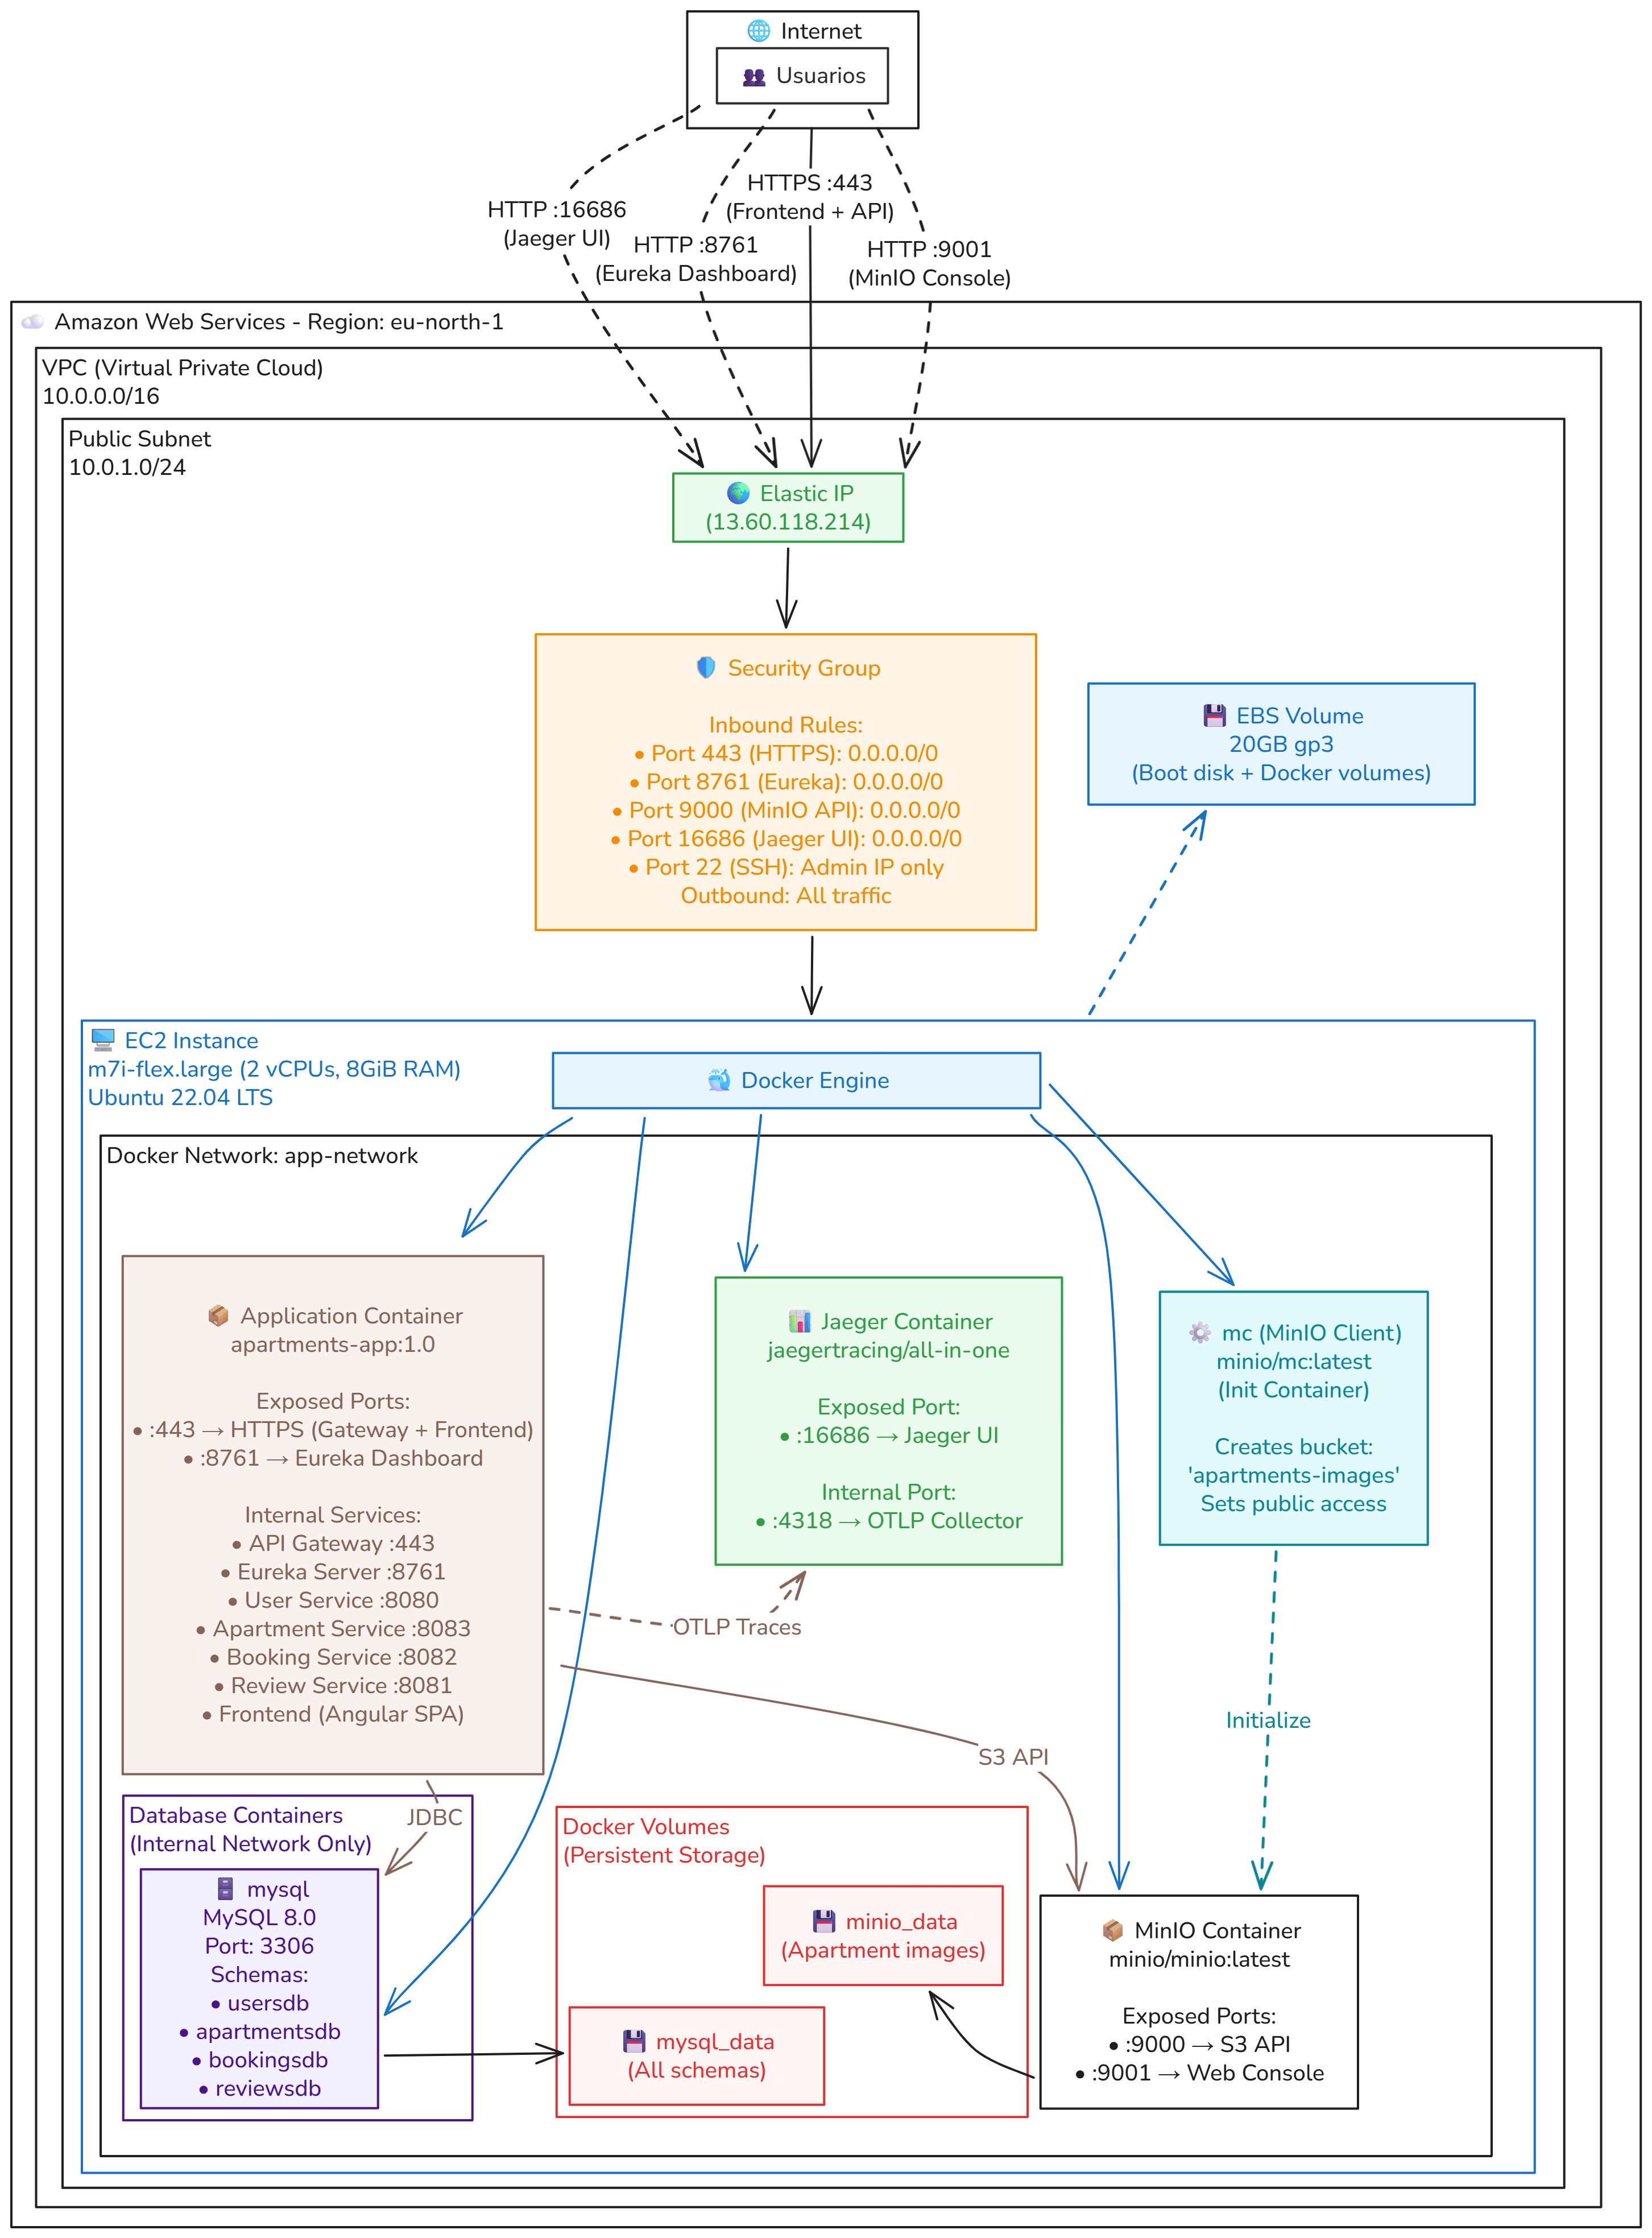
\includegraphics[width=\textwidth]{img/diagrama_despliegue.png}
\caption{Arquitectura de despliegue en Amazon EC2.}
\label{fig:despliegue_aws}
\end{figure}

\subsubsection{Arquitectura de Infraestructura}
La infraestructura consta de los siguientes componentes clave diseñados para garantizar 
el aislamiento y la seguridad:
\begin{itemize}
    \item \textbf{Instancia EC2 (m7i-flex.large):} Máquina con Ubuntu 22.04 LTS, 2 vCPUs 
    y 8 GiB de RAM para soportar las exigencias de memoria de la JVM.
    \item \textbf{Elastic IP:} Dirección IPv4 pública y estática (13.60.118.214).
    \item \textbf{Security Group (Firewall):} Expone el puerto 443 (HTTPS) al público, 
    reserva el 22 (SSH) para el administrador, y habilita los puertos 8761, 9001 y 16686 
    excepcionalmente para la evaluación académica del proyecto.
\end{itemize}

\subsubsection{Procedimiento de Despliegue}
El uso de artefactos OCI (\textit{Open Container Initiative}) hace que el despliegue sea 
altamente predecible y no requiera clonar el código fuente. Tras aprovisionar la máquina 
e instalar Docker, el administrador configura las credenciales y parámetros de 
infraestructura mediante un archivo de variables de entorno \texttt{.env}. El formato 
detallado de este archivo, así como la descripción de todas las variables disponibles, 
se detallan en el Anexo~\ref{anexo:instrucciones-ejecutar-aplicacion}.

Una vez configurado el entorno, se ejecuta un único comando que descarga el manifiesto 
directamente desde DockerHub:

\begin{verbatim}
docker compose -f oci://eloydsdlh/apartments-compose:1.0 up -d
\end{verbatim}

Este comando automatiza la descarga de imágenes, la creación de redes, la inicialización 
de los esquemas de base de datos y el inicio jerárquico dictado por los \textit{healthchecks} 
(levantando primero MySQL y MinIO antes que la aplicación principal). En cuestión de minutos, 
el orquestador registra los microservicios en Eureka y levanta el \textit{API Gateway}, dejando la 
aplicación operativa y accesible de forma segura.

\section{Proceso de Desarrollo} 
\label{sec:proceso_desarrollo}

El desarrollo se ha regido por un proceso \textbf{iterativo e incremental}, fuertemente alineado con los principios del Manifiesto Ágil ~\cite{ManifiestoAgil}. Se ha priorizado la entrega continua de valor, la adaptación al cambio y la automatización de procesos. Para ello, el proyecto se ha apoyado en prácticas fundamentales de la Programación Extrema (XP) ~\cite{Beck1999}, tales como la integración continua, el diseño guiado por pruebas automatizadas y las iteraciones cortas de desarrollo. 

La gestión del flujo de trabajo se ha fundamentado en metodologías visuales basadas en Kanban. Cabe destacar de manera explícita que no se ha aplicado el marco de trabajo Scrum, dado que sus ceremonias y artefactos no se adecúan a la naturaleza de un proyecto individual de esta índole.

\subsection{Gestión de Tareas} 
La planificación y el seguimiento del trabajo se han centralizado utilizando las herramientas nativas del repositorio: \textbf{GitHub Issues} y \textbf{GitHub Projects}. 

\begin{itemize}
    \item \textbf{GitHub Issues:} Se han utilizado como la unidad básica de trabajo, registrando en ellos los requisitos funcionales, la detección de errores (\textit{bugs}), mejoras técnicas y nuevas características.
    \item \textbf{GitHub Projects:} Ha proporcionado la capa de gestión visual. Mediante un tablero \textbf{Kanban}, los \textit{issues} se organizaron en columnas de estado (\textit{To Do}, \textit{In Progress}, \textit{Done}), permitiendo una priorización clara de las tareas y una monitorización en tiempo real del progreso del desarrollo. El tablero de gestión del proyecto es accesible en:
    \newline
    \url{https://github.com/orgs/codeurjc-students/projects/16}
\end{itemize}

Para analizar el progreso del proyecto a lo largo del tiempo, se ha utilizado un gráfico de \textit{Burn up} (Figura \ref{fig:burnup_chart}) extraído directamente de las analíticas del repositorio. Este gráfico ilustra la evolución del alcance del proyecto (tareas abiertas) frente a la velocidad de resolución (tareas completadas), evidenciando la naturaleza iterativa y adaptativa de la metodología empleada.

\begin{figure}[!h]
    \centering
    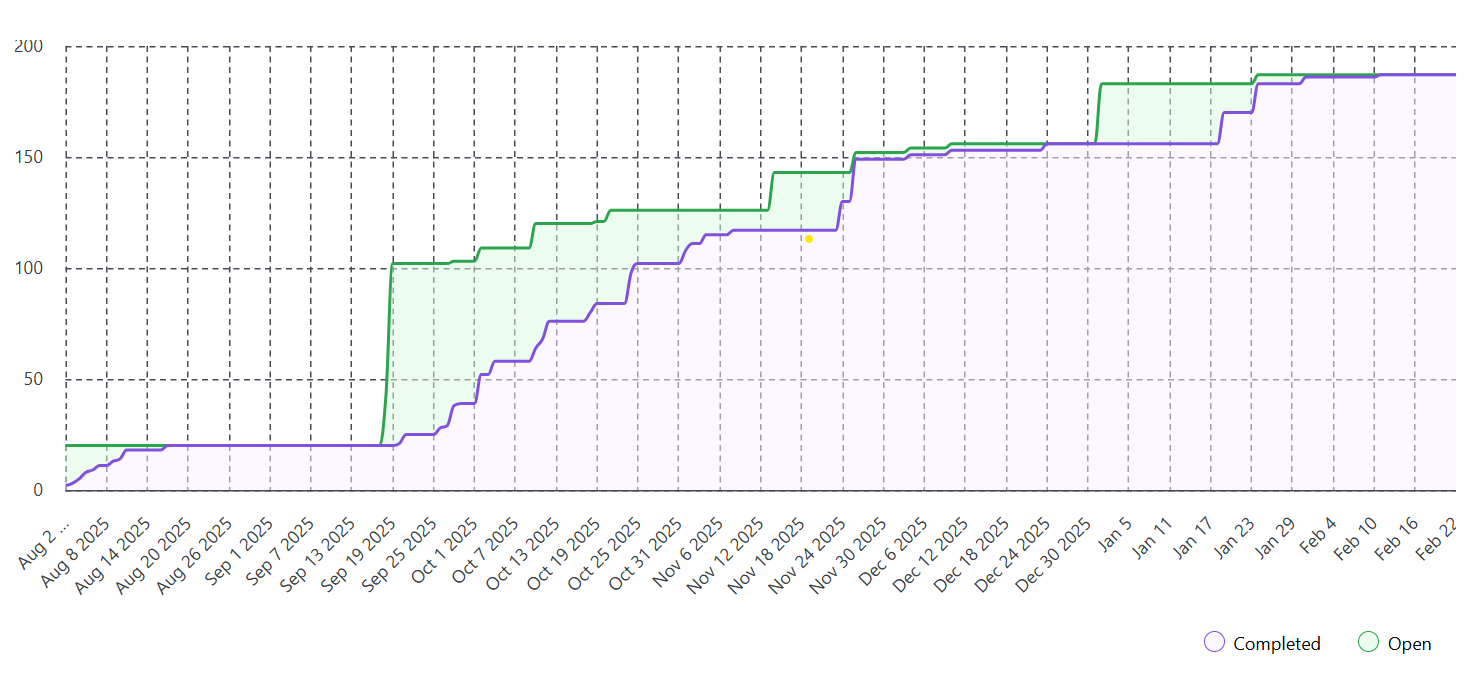
\includegraphics[width=\textwidth]{img/burnup_chart.png}
    \caption{Gráfico de Burn up del proyecto. La línea superior (verde) representa el total de tareas identificadas y la línea inferior (morada) las tareas completadas a lo largo del tiempo.}
    \label{fig:burnup_chart}
\end{figure}

\subsection{Control de Versiones con Git} 
El control de versiones del código fuente se ha gestionado íntegramente con \textbf{Git}, y el repositorio del proyecto se encuentra alojado públicamente en GitHub: \newline
\url{https://github.com/codeurjc-students/2025-sky-apartments}.\newline
Para garantizar la estabilidad del código, se ha implementado una estrategia de ramificación (\textit{branching strategy}) estricta basada en el modelo de \textit{feature branches}:

\begin{itemize}
    \item \textbf{Rama \texttt{main}:} Rama principal protegida. Contiene código estable y siempre listo para ser desplegado.
    \item \textbf{Ramas de característica (\texttt{feature/*}):} Creadas a partir de \texttt{main} para desarrollar de forma aislada cada nueva funcionalidad.
    \item \textbf{Ramas de corrección (\texttt{fix/*}):} Destinadas exclusivamente a la resolución de errores detectados.
    \item \textbf{Ramas auxiliares (\texttt{testing/*}, \texttt{ci/*}, \texttt{docs/*}):} Utilizadas para la configuración de flujos de trabajo, pruebas de integración continua y redacción de documentación.
\end{itemize}

La integración de código hacia la rama \texttt{main} se ha realizado exclusivamente mediante \textbf{Pull Requests} (PR), forzando la revisión de código y la ejecución de los flujos de integración continua antes de permitir la fusión. 

A la fecha de cierre de este documento, el repositorio cuenta con un histórico sólido y altamente estructurado, registrando un total de \textbf{346 \textit{commits}}, \textbf{67 ramas} creadas para aislar el trabajo y \textbf{63 \textit{Pull Requests}}.

\subsection{Integración y Entrega Continua (CI)} 
La automatización de la calidad del código se ha orquestado mediante \textbf{GitHub Actions}, definiendo múltiples flujos de trabajo que actúan como barreras de calidad en diferentes etapas.
\subsubsection{Basic Quality Check}
Se ejecuta con cada (\textit{push}) a las ramas de desarrollo. Su objetivo es proporcionar retroalimentación rápida al desarrollador:
\begin{itemize}
    \item \textbf{\texttt{backend-basic}:} Ejecuta las pruebas unitarias aisladas para todos los microservicios Java (Apartment, User, Booking, Review).
    \item \textbf{\texttt{frontend-basic}:} Instala dependencias y ejecuta la suite de pruebas unitarias de Angular.
\end{itemize}

\subsubsection{Full Quality Check}
Se activa al abrir o actualizar una \textit{Pull Request} hacia la rama \texttt{main}. Es un flujo exhaustivo y secuencial que levanta toda la infraestructura para validar el sistema en su conjunto:
\begin{enumerate}
    \item \textbf{\texttt{backend-unit-integration}:} Ejecuta pruebas unitarias y de integración del backend, utilizando \textbf{Testcontainers} para levantar bases de datos MySQL efímeras.
    \item \textbf{\texttt{backend-e2e}:} Tras compilar los microservicios, utiliza Docker Compose para levantar la infraestructura completa (Bases de datos, MinIO, Eureka, Gateway, Jaeger y microservicios). Valida la comunicación cruzada entre servicios ejecutando pruebas End-to-End en el backend, esperando a que todos los servicios se registren sanos en Eureka.
    \item \textbf{\texttt{frontend-integration}:} Ejecuta pruebas de integración en el cliente web conectándose a los microservicios levantados en el paso anterior a través del \textit{API Gateway}.
    \item \textbf{\texttt{frontend-e2e}:} Instala los navegadores de \textbf{Playwright}, arranca el servidor de desarrollo de Angular y simula interacciones reales de usuario, validando flujos completos desde la interfaz gráfica hasta la base de datos.
    \item \textbf{\texttt{frontend-unit}:} Ejecuta la suite de pruebas unitarias del cliente web mediante Karma y Jasmine para validar la lógica aislada.
\end{enumerate}

Toda esta infraestructura efímera inyecta las variables de entorno mediante los \textit{Secrets} de GitHub de forma segura y destruye los contenedores tras finalizar las pruebas, garantizando un entorno limpio en cada ejecución.

\subsection{Entrega Continua y Versionado} 
El proyecto emplea un sistema de \textbf{entrega continua} automatizado mediante GitHub Actions para publicar las imágenes en DockerHub. El paso a producción (AWS) se realiza de forma manual y controlada, rigiéndose por un \textbf{versionado semántico} gestionado a través de \textit{Releases} de GitHub.

\subsubsection{Gestión de Versiones y Publicación}
Los \textit{merges} en \texttt{main} generan automáticamente la imagen \texttt{:dev}, mientras que al crear una \textit{Release} se sincronizan las versiones internas (\texttt{pom.xml}, \texttt{package.json}) y se publican las imágenes definitivas etiquetadas con su versión (ej. \texttt{:0.1}) y como \texttt{:latest}.


\subsubsection{Historial de Lanzamientos}
A lo largo del proyecto se han publicado tres iteraciones mayores:
\begin{itemize}
    \item \textbf{08/11/2025 -- v0.1 (MVP Técnico):} Cimientos arquitectónicos, seguridad (HTTPS), despliegue inicial con Docker y CRUD básico de usuarios, apartamentos y reservas.
    \item \textbf{24/12/2025 -- v0.2 (UX y Cloud):} Despliegue oficial en AWS EC2. Integró galerías (MinIO), calendarios en tiempo real, emails automatizados, reseñas y el \textit{Dashboard} administrativo.
    \item \textbf{01/02/2026 -- v1.0 (Lógica Avanzada):} Versión final. Introdujo el motor de precios dinámicos, recordatorios automáticos de \textit{check-in} y filtrado avanzado.
\end{itemize}

\subsubsection{Impacto en los usuarios durante el despliegue}
El despliegue sobre Amazon EC2 conlleva un breve \textit{downtime} planificado: el administrador ejecuta \texttt{docker compose down} y \texttt{docker compose up -d} para descargar las nuevas imágenes e iniciar los servicios. Esta sustitución directa, aunque implica unos minutos de inactividad, es adecuada para la escala académica del proyecto.

\blankpage

% Capítulo 5

\chapter{Conclusiones y trabajos futuros}

La culminación de este Trabajo de Fin de Grado permite realizar una evaluación global sobre el cumplimiento de las metas iniciales, el proceso de desarrollo y los conocimientos adquiridos.
\section{Conclusiones}
El objetivo principal era diseñar e implementar un sistema completo de gestión de apartamentos turísticos con arquitectura de microservicios, integrando backend y frontend, y desplegándolo en un entorno de producción real. Este objetivo se ha cumplido satisfactoriamente.
\subsection{Materialización de los Objetivos Funcionales}
Desde la perspectiva del negocio y del usuario, los objetivos funcionales se han cumplido con éxito mediante la entrega de \textbf{Sky Apartments}, una plataforma web plenamente operativa. Se ha logrado materializar:
\begin{itemize}
    \item \textbf{Una experiencia de usuario completa:} Implementando un catálogo interactivo, filtros avanzados y un calendario de disponibilidad en tiempo real que evita problemas críticos como el \textit{overbooking}.
    \item \textbf{Autonomía operativa:} A través de un motor de reservas automatizado, el sistema de notificaciones transaccionales por correo electrónico y el módulo de reseñas y valoraciones.
    \item \textbf{Gestión centralizada:} Mediante un panel de administración que permite controlar el catálogo y aplicar reglas de precios dinámicos altamente flexibles, logrando la ansiada independencia tecnológica respecto a plataformas de terceros.
\end{itemize}

\subsection{Materialización de los Objetivos Técnicos}
A nivel tecnológico, el proyecto ha superado el alcance de una aplicación monolítica tradicional, materializándose en una arquitectura distribuida moderna y robusta:
\begin{itemize}
    \item \textbf{Arquitectura de Microservicios:} Se ha implementado un ecosistema basado en Spring Boot orquestado con API Gateway y Eureka, aplicando rigurosamente patrones de diseño distribuido. El patrón \textit{Database per Service}~\cite[Cap.~5]{richardson2018}, por el que cada microservicio mantiene su propia base de datos MySQL aislada, es una condición esencial de esta arquitectura y ha sido aplicado de forma rigurosa.
    \item \textbf{Despliegue y DevOps:} El empaquetado en contenedores Docker y la automatización del flujo CI/CD mediante GitHub Actions han permitido un despliegue exitoso en Amazon EC2 (AWS).
    \item \textbf{Calidad de Software:} Una estrategia de pruebas exhaustiva ha permitido alcanzar coberturas superiores al 85\% en el backend y 90\% en el frontend, garantizando la mantenibilidad futura.
\end{itemize}

\subsection{Reflexión Personal}
El desarrollo de este proyecto ha constituido una experiencia de aprendizaje extraordinariamente enriquecedora. La arquitectura de microservicios demostró ventajas evidentes, pero también reveló la inmensa complejidad inherente a la coordinación y depuración distribuida. 

Comprender que la observabilidad (mediante Jaeger) y la infraestructura son pilares críticos ha sido fundamental. Con la perspectiva adquirida y evaluando los \textit{trade-offs}\footnote{En ingeniería de software, un \textit{trade-off} es una decisión de diseño donde elegir una solución implica renunciar a ciertos atributos (ej. simplicidad) en favor de otros beneficios (ej. escalabilidad).}, reconozco que en ciertos escenarios un monolito modular podría ser un punto de partida más pragmático para evitar una complejidad prematura~\cite{newman2015}. 

No obstante, superar los retos de integración externa, algoritmos de \textit{pricing} y despliegue \textit{cloud}, ha consolidado competencias técnicas directamente aplicables al mundo profesional.


\section{Trabajos futuros}
\label{sec:trabajos_futuros}

Aunque el sistema es plenamente funcional y se encuentra en producción, la base arquitectónica diseñada permite una evolución continua.

\subsection{Mejoras Funcionales}
\begin{itemize}
    \item \textbf{Pasarela de Pagos Segura:} Integración con Stripe o PayPal\footnote{Stripe: \url{https://stripe.com/docs/api}, PayPal: \url{https://developer.paypal.com/}} para procesar transacciones económicas reales.
    \item \textbf{Experiencia de Usuario:} Inicio de sesión mediante redes sociales (OAuth 2.0)\footnote{OAuth 2.0, RFC 6749: \url{https://tools.ietf.org/html/rfc6749}} y soporte multi-idioma.
    \item \textbf{Inteligencia Artificial aplicada al Negocio:} Sustitución del motor de reglas manual por un modelo predictivo de \textit{Machine Learning} que optimice las tarifas aplicando técnicas de \textit{revenue management}~\cite{talluri2004revenue} basadas en demanda histórica y estacionalidad.
\end{itemize}

\subsection{Mejoras Técnicas}
\begin{itemize}
    \item \textbf{Optimización del Rendimiento:} Implementación de una caché distribuida (como Redis\footnote{Redis: \url{https://redis.io/}}) para reducir la carga de la base de datos en consultas recurrentes.
    \item \textbf{Tolerancia a Fallos:} Transición hacia arquitecturas orientadas a eventos (\textit{message brokers} como RabbitMQ\footnote{RabbitMQ: \url{https://www.rabbitmq.com/}}) para desacoplar operaciones no bloqueantes, e integración de patrones \textit{Circuit Breaker}~\cite{nygard2007release} para evitar fallos en cascada.
    \item \textbf{Evolución del Despliegue:} Separar la imagen Docker única en contenedores independientes por microservicio y migrar la orquestación a \textbf{Kubernetes\footnote{Kubernetes (K8s): \url{https://kubernetes.io/}} (K8s)}, habilitando el escalado horizontal elástico e independiente de cada servicio según la demanda.
\end{itemize}

\blankpage


%%%%%%%%%%%%%%%%%%%%%%%%%%%%%%% Bibliografía %%%%%%%%%%%%%%%%%%%%%%%%%%%%%%%

\phantomsection
\addcontentsline{toc}{chapter}{Bibliografía}

\footnotesize{
%\bibliographystyle{hispa}
\bibliographystyle{IEEEtran}
\bibliography{bibliografia}
}

\normalsize

% No expandir elementos para llenar toda la página
\raggedbottom
\afterpage{\blankpage}

\newpage




%%%%%%%%%%%%%%%%%%%%%%%%%%%%%%% Anexos %%%%%%%%%%%%%%%%%%%%%%%%%%%%%%%

\appendix

\phantomsection
\addcontentsline{toc}{chapter}{Anexos}

\mbox{}
\vfill
\begin{center}
\begin{Huge}
\textbf{Anexos}
\end{Huge}
\end{center}
\vfill
\mbox{}
\thispagestyle{empty}

\newpage
\mbox{}
\thispagestyle{empty}
\newpage


% Primer anexo
\chapter{Funcionalidades detalladas}
\label{anexo:funcionalidades-detalladas}
A continuación se detalla el desglose técnico y funcional de todas las características implementadas en la plataforma \textbf{Sky Apartments}, categorizadas por su nivel de complejidad y alcance operativo.

\section{Funcionalidades Básicas}

\subsubsection{Gestión de Usuarios Anónimos:}
\begin{itemize}
    \item Visualización del catálogo general de apartamentos.
    \item Filtrado básico por capacidad (número de huéspedes).
    \item Filtrado por comodidades específicas (terraza, balcón, ubicación, etc.).
    \item Acceso a la vista de detalle del apartamento (fotografías, descripción, precio por noche).
    \item Consulta de disponibilidad en el calendario sin necesidad de autenticación.
\end{itemize}

\subsubsection{Gestión de Usuarios Registrados:}
\begin{itemize}
    \item Registro de nuevas cuentas (\textit{Sign Up}) con validación de formato de correo electrónico y contraseña segura.
    \item Autenticación segura (\textit{Log In}) mediante Spring Security y contraseñas encriptadas.
    \item Visualización y edición de datos del perfil personal.
    \item Realización de reservas en apartamentos con disponibilidad.
    \item Visualización del historial completo de reservas personales.
    \item Cancelación de reservas activas.
\end{itemize}

\subsubsection{Gestión de Administradores:}
\begin{itemize}
    \item Autenticación segura mediante credenciales predefinidas.
    \item Operaciones CRUD completas (Crear, Leer, Actualizar, Eliminar) sobre el catálogo de apartamentos.
    \item Gestión y subida de imágenes principales para los alojamientos.
    \item Visualización general de todas las reservas registradas en el sistema.
\end{itemize}

\section{Funcionalidades Intermedias}

\subsubsection{Búsqueda y Visualización:}
\begin{itemize}
    \item Motor de búsqueda avanzado con combinación simultánea de múltiples filtros (fechas, comodidades, capacidad).
    \item Soporte para múltiples imágenes por apartamento (Galería multimedia).
    \item Visualización interactiva de la disponibilidad mediante un componente de calendario.
    \item Geolocalización básica de los apartamentos.
\end{itemize}


\subsubsection{Comunicaciones y Experiencia de Usuario:}
\begin{itemize}
    \item Envío automatizado de correos electrónicos transaccionales para la confirmación de reservas.
    \item Sistema de reseñas: posibilidad de valorar la estancia y dejar comentarios de texto.
    \item Páginas de error personalizadas (403, 404, 500, 503) integradas con el diseño general de la aplicación.
\end{itemize}

\section{Funcionalidades Avanzadas}

\subsubsection{Analítica de Negocio (Dashboard Interactivo):}
\begin{itemize}
    \item Gráficos dinámicos de ingresos y reservas por mes.
    \item Estadísticas de ocupación media y duración de las estancias.
    \item Ranking visual de los alojamientos más demandados.
    \item Ranking de los apartamentos con mejores valoraciones.
\end{itemize}


\subsubsection{Motor de Precios Dinámicos y Lógica Avanzada:}

\begin{itemize}
    \item Modificadores de precio automatizados basados en:
    \begin{itemize}
        \item Temporadas del año (Baja, Media, Alta).
        \item Día de la semana (Incrementos en fines de semana).
        \item Proximidad de la fecha de reserva (descuentos \textit{last-minute} o recargos por anticipación).
    \end{itemize}
    \item Desglose transparente del precio base frente a los modificadores aplicados en el momento de la confirmación de la reserva.
    \item Envío de correos electrónicos automatizados de recordatorio de \textit{check-in} en fechas próximas a la llegada.
\end{itemize}

% Segundo anexo
\chapter{Instrucciones para ejecutar la aplicación}
\label{anexo:instrucciones-ejecutar-aplicacion}
Esta guía proporciona las instrucciones detalladas paso a paso para ejecutar la versión 1.0 de \textbf{Sky Apartments} utilizando Docker Compose.

\section{Requisitos Previos}

\subsection{Instalación de Docker}
La aplicación requiere el uso de \textbf{Docker} para su ejecución. Las instrucciones de instalación varían en función del sistema operativo:

\subsubsection*{Windows}
\begin{itemize}
    \item Descargar e instalar \textbf{Docker Desktop para Windows}.
    \item Enlace oficial: \url{https://docs.docker.com/desktop/install/windows-install/}
    \item Requisitos del sistema: Windows 10 de 64 bits o superior.
\end{itemize}

\subsubsection*{macOS}
\begin{itemize}
    \item Descargar e instalar \textbf{Docker Desktop para Mac}.
    \item Enlace oficial: \url{https://docs.docker.com/desktop/install/mac-install/}
    \item Disponible tanto para procesadores Intel como para Apple Silicon.
\end{itemize}

\subsubsection*{Linux}
Es necesario instalar tanto \textbf{Docker Engine} como \textbf{Docker Compose}:

\begin{itemize}
    \item \textbf{Docker Engine:} Visitar \url{https://docs.docker.com/engine/install/} y seleccionar la distribución de Linux correspondiente (Ubuntu, Debian, Fedora, etc.).
    \item \textbf{Docker Compose:} Visitar \url{https://docs.docker.com/compose/install/} y seguir los pasos de instalación para Docker Compose independiente (\textit{standalone}).
\end{itemize}

\subsection{Verificación de la instalación}
Una vez finalizada la instalación, se puede verificar que Docker funciona correctamente abriendo un terminal y ejecutando:

\begin{lstlisting}[language=bash, basicstyle=\ttfamily\small]
docker --version
docker compose version
\end{lstlisting}

\section{Ejecución de la Aplicación}

\subsection{Opción 1: Mediante registro de DockerHub (Recomendada)}
Esta opción utiliza el artefacto OCI directamente sin necesidad de descargar archivos manuales:
\begin{lstlisting}[language=bash, basicstyle=\ttfamily\small]
docker compose -f oci://eloydsdlh/apartments-compose:1.0 up -d
\end{lstlisting}
\textit{Nota: Puede sustituir \texttt{1.0} por cualquier tag disponible en el registro oficial (\url{https://hub.docker.com/r/eloydsdlh/apartments-compose/tags}).}

\subsection{Opción 2: Mediante archivo docker-compose.yml}

\begin{enumerate}
    \item \textbf{Descargar el archivo \texttt{docker-compose.yml}} \\
    Se puede descargar directamente desde el repositorio o crearlo manualmente ejecutando:
\begin{lstlisting}[language=bash, basicstyle=\ttfamily\small]
curl -o docker-compose.yml \
  https://raw.githubusercontent.com/codeurjc-students/\
  2025-sky-apartments/main/docker/docker-compose.yml
\end{lstlisting}

    \item \textbf{Iniciar la aplicación}
\begin{lstlisting}[language=bash, basicstyle=\ttfamily\small]
docker compose up -d
\end{lstlisting}
    Este comando se encargará de:
    \begin{itemize}
        \item Descargar la imagen de Sky Apartments desde DockerHub (etiqueta: \texttt{1.0}).
        \item Descargar la imagen de MySQL.
        \item Crear y arrancar los contenedores.
        \item Configurar la red interna para su comunicación.
    \end{itemize}

    \item \textbf{Esperar al arranque de la aplicación} \\
    La primera vez que se ejecute, el proceso puede tardar unos minutos mientras se descargan las imágenes, se inicializa la base de datos y se cargan los datos de prueba. Se puede monitorizar el progreso con:
\begin{lstlisting}[language=bash, basicstyle=\ttfamily\small]
docker compose logs -f
\end{lstlisting}

    \item \textbf{Acceder a la aplicación} \\
    Una vez que los registros (\textit{logs}) muestren que la aplicación ha arrancado correctamente, se debe abrir el navegador web y acceder a:\newline \url{https://localhost} \\
    
    \textit{\textbf{Nota:}} Es posible que el navegador muestre una advertencia de seguridad debido al uso de un certificado SSL autofirmado (comportamiento esperado en entornos de desarrollo). Para continuar, se debe hacer clic en "Avanzado" y luego en "Aceptar el riesgo y continuar" (o equivalente según el navegador).
\end{enumerate}

\section{Variables de Entorno}
Para el correcto funcionamiento de las \textbf{notificaciones por correo}, cree un archivo \texttt{.env} en el directorio raíz:

\begin{table}[H]
\centering
\begin{tabular}{@{}lll@{}}
\toprule
\textbf{Variable} & \textbf{Requerido} & \textbf{Descripción} \\ \midrule
\texttt{MAIL\_USERNAME} & Sí & Cuenta de correo emisor. \\
\texttt{MAIL\_PASSWORD} & Sí & Contraseña de aplicación del correo. \\
\texttt{JWT\_SECRET}    & No & Clave para tokens (recomendado cambiar). \\ \bottomrule
\end{tabular}
\caption{Variables de configuración principales.}
\end{table}

Ejemplo de archivo \texttt{.env} con todas las variables (necesarias y opcionales):
\begin{lstlisting}
# --- Email (Requerido para notificaciones) ---
MAIL_USERNAME=ejemplo@gmail.com
MAIL_PASSWORD=tu_password_secreto

# --- Base de Datos (MySQL) ---
MYSQL_ROOT_PASSWORD=password
MYSQL_USER=user
MYSQL_PASSWORD=password
MYSQL_USERS_DB=usersdb
MYSQL_APARTMENTS_DB=apartmentsdb
MYSQL_BOOKINGS_DB=bookingsdb
MYSQL_REVIEWS_DB=reviewsdb

# --- Almacenamiento de imagenes (MinIO) ---
MINIO_ROOT_USER=minioadmin
MINIO_ROOT_PASSWORD=minioadmin
MINIO_BUCKET=apartments-images
MINIO_EXTERNAL_URL=https://localhost:443/minio

# --- Seguridad y JWT (Se recomienda cambiar en produccion) ---
JWT_SECRET=Xv5s7JxGg9YhQwD8M1lA0VhG7yJrL6hE9F1N8KxV2bW3ZpQxUsyR7Cj4KsE8YfHd

# --- Configuracion SSL ---
SSL_KEY_STORE=classpath:keystore.p12
SSL_KEY_STORE_PASSWORD=changeit
SSL_KEY_STORE_TYPE=PKCS12
SSL_KEY_ALIAS=apartments

# --- Perfil del Sistema ---
SPRING_PROFILE=prod
\end{lstlisting}

\section{Acceso a la Aplicación y Datos de Prueba}

\subsection{Interfaz Web}
La interfaz web es accesible a través del navegador en:\newline \url{https://localhost}

\subsection{Credenciales de acceso}
La aplicación incluye datos preconfigurados para facilitar las pruebas.

\subsubsection*{Acceso de Administrador}
\begin{itemize}
    \item \textbf{Usuario:} \texttt{admin@example.com}
    \item \textbf{Contraseña:} \texttt{Password@1234}
\end{itemize}
La cuenta de administrador cuenta con acceso completo a la gestión de apartamentos (crear, editar, eliminar), gestión de usuarios y estadísticas del sistema.

\subsubsection*{Cuentas de Usuario Estándar}
Se pueden crear cuentas propias o utilizar la cuenta de prueba existente:
\begin{itemize}
    \item \textbf{Usuario:} \texttt{user@example.com}
    \item \textbf{Contraseña:} \texttt{Password@1234}
\end{itemize}

\subsection{Datos de ejemplo incluidos}
La base de datos arranca con los siguientes elementos preconfigurados:
\begin{itemize}
    \item \textbf{10 apartamentos:} Incluyen nombre, descripción, capacidad máxima, combinaciones de comodidades (terraza, parking, piscina, etc.), imágenes representativas y precio por noche.
    \item \textbf{Reservas:} Muestra de reservas activas y pasadas.
    \item \textbf{Reseñas:} Comentarios de ejemplo para ilustrar el sistema de valoraciones.
\end{itemize}

\section{Administración de la Aplicación}

\subsubsection*{Detener la aplicación}
\begin{lstlisting}[language=bash, basicstyle=\ttfamily\small]
docker compose down
\end{lstlisting}
Este comando detiene y elimina los contenedores, pero \textbf{conserva} los datos de la base de datos.

\subsubsection*{Detener y eliminar todos los datos}
\begin{lstlisting}[language=bash, basicstyle=\ttfamily\small]
docker compose down -v
\end{lstlisting}
\textit{\textbf{Advertencia:}} Esto eliminará todos los datos, incluida la base de datos. En el próximo arranque, se volverán a cargar los datos de prueba iniciales.

\subsubsection*{Visualizar registros (Logs)}
\begin{lstlisting}[language=bash, basicstyle=\ttfamily\small]
# Todos los servicios
docker compose logs

# Seguir logs en tiempo real
docker compose logs -f

# Servicio especifico
docker compose logs app
docker compose logs db
\end{lstlisting}

\subsubsection*{Reiniciar y actualizar}
\begin{lstlisting}[language=bash, basicstyle=\ttfamily\small]
# Reiniciar la aplicacion
docker compose restart

# Actualizar a la ultima version
docker compose pull
docker compose up -d
\end{lstlisting}

\section{Resolución de Problemas}

\subsection{Puerto ya en uso}
Si los puertos 443 o 3306 ya están en uso, se mostrará un error. Posibles soluciones:
\begin{enumerate}
    \item \textbf{Detener servicios en conflicto:} Detener cualquier servidor web (Apache, Nginx) que use el puerto 443 o servicio MySQL/MariaDB en el puerto 3306.
    \item \textbf{Modificar puertos en \texttt{docker-compose.yml}:}
\begin{lstlisting}[language=bash, basicstyle=\ttfamily\small]
services:
  app:
    ports:
      - "8443:443"  # Usar el puerto 8443 en su lugar
\end{lstlisting}
    Tras el cambio, se accederá a través de: \url{https://localhost:8443}
\end{enumerate}

\subsection{Problemas de conexión a la base de datos}
Si la aplicación no logra conectar con la base de datos:
\begin{enumerate}
    \item Esperar unos segundos más (la base de datos necesita tiempo para inicializarse).
    \item Comprobar los logs de la base de datos: \texttt{docker compose logs db}
    \item Reiniciar los servicios: \texttt{docker compose restart}
\end{enumerate}

\subsection{La aplicación no carga}
\begin{enumerate}
    \item Comprobar si los contenedores están en ejecución: \texttt{docker compose ps}
    \item Revisar los logs de la aplicación: \texttt{docker compose logs app}
    \item Vaciar la caché del navegador o probar en modo incógnito.
\end{enumerate}

\section{Versión de Desarrollo}
Para ejecutar la última versión de desarrollo (puede ser inestable):
\begin{lstlisting}[language=bash, basicstyle=\ttfamily\small]
# Descargar docker-compose-dev.yml
curl -o docker-compose-dev.yml \
 https://raw.githubusercontent.com/codeurjc-students/\
 2025-sky-apartments/main/docker/docker-compose-dev.yml

# Ejecutar version de desarrollo
docker compose -f docker-compose-dev.yml up -d
\end{lstlisting}
Esta versión utiliza la etiqueta \texttt{dev} de DockerHub e incluye las últimas funcionalidades en pruebas.

\section{Recursos Adicionales}
\begin{itemize}
    \item \textbf{Documentación de Docker:} \url{https://docs.docker.com}
    \item \textbf{Documentación de Docker Compose:} \url{https://docs.docker.com/compose/}
    \item \textbf{Repositorio del proyecto:} \url{https://github.com/codeurjc-students/2025-sky-apartments}
\end{itemize}

% Tercer anexo
\chapter{Ejecución y edición de código}
\label{anexo:ejecucion-edicion-codigo}
Este anexo detalla las instrucciones necesarias para clonar el repositorio, configurar el entorno de desarrollo local y ejecutar las pruebas de \textbf{Sky Apartments}.

\section{Configuración del Repositorio}
Para clonar el repositorio del proyecto en el equipo local, se debe ejecutar el siguiente comando:

\begin{lstlisting}[language=bash]
git clone https://github.com/codeurjc-students/2025-sky-apartments.git
cd 2025-sky-apartments
\end{lstlisting}

\section{Ejecución con Docker Compose (Recomendado)}
La forma más sencilla de ejecutar la aplicación completa con todos sus servicios es utilizando Docker Compose.

\subsection{Versión Estable}
\begin{lstlisting}[language=bash]
cd docker
docker compose up
\end{lstlisting}
Este comando realizará las siguientes acciones:
\begin{itemize}
    \item Descargar la última imagen estable desde DockerHub.
    \item Iniciar contenedores MySQL independientes para cada microservicio.
    \item Iniciar MinIO para el almacenamiento de objetos.
    \item Iniciar Eureka Server para el descubrimiento de servicios.
    \item Iniciar todos los microservicios de la lógica de negocio (Usuarios, Apartamentos, Reservas, Reseñas).
    \item Iniciar el API Gateway con configuración HTTPS.
    \item Iniciar Jaeger para la trazabilidad distribuida.
    \item Desplegar el \textit{frontend} accesible en \url{https://localhost/}.
\end{itemize}

\subsection{Versión de Desarrollo}
Para probar los últimos cambios integrados en la rama principal (\texttt{main}), se puede utilizar la versión de desarrollo:
\begin{lstlisting}[language=bash]
cd docker
docker compose -f docker-compose-dev.yml up
\end{lstlisting}

\subsection{Accesos a los servicios}
Una vez levantada la infraestructura, los distintos servicios son accesibles a través de las siguientes rutas:
\begin{itemize}
    \item \textbf{Frontend:} \url{https://localhost/}
    \item \textbf{API Gateway:} \url{https://localhost/api/}
    \item \textbf{Panel de Eureka:} \url{http://localhost:8761/}
    \item \textbf{Interfaz de Jaeger:} \url{http://localhost:16686/}
    \item \textbf{Consola de MinIO:} \url{http://localhost:9001/}
\end{itemize}

\section{Ejecución Manual (Entorno de Desarrollo Local)}
Para modificar el código y realizar desarrollo local sin empaquetar en contenedores Docker la propia aplicación, se deben seguir estos pasos.

\subsection{Requisitos Previos}
\begin{itemize}
    \item \textbf{Java:} Versión 17.
    \item \textbf{Node.js:} Versión 20.18.0.
    \item \textbf{MySQL:} Versión 8.0 (mediante Docker o instalación nativa).
    \item \textbf{MinIO:} Para almacenamiento de objetos (mediante Docker).
    \item \textbf{Maven Wrapper:} Incluido en el propio repositorio.
\end{itemize}

\subsection{Configuración de Bases de Datos}
Se deben arrancar los contenedores de MySQL para cada microservicio ejecutando:

\begin{lstlisting}[language=bash]
# Base de datos del Servicio de Usuarios (Puerto 3307)
docker run --name mysql-user -e MYSQL_ROOT_PASSWORD=root -e MYSQL_DATABASE=user_db -e MYSQL_USER=user -e MYSQL_PASSWORD=password -p 3307:3306 -d mysql:8.0

# Base de datos del Servicio de Apartamentos (Puerto 3308)
docker run --name mysql-apartment -e MYSQL_ROOT_PASSWORD=root -e MYSQL_DATABASE=apartment_db -e MYSQL_USER=user -e MYSQL_PASSWORD=password -p 3308:3306 -d mysql:8.0

# Base de datos del Servicio de Reservas (Puerto 3309)
docker run --name mysql-booking -e MYSQL_ROOT_PASSWORD=root -e MYSQL_DATABASE=booking_db -e MYSQL_USER=user -e MYSQL_PASSWORD=password -p 3309:3306 -d mysql:8.0

# Base de datos del Servicio de Resenas (Puerto 3310)
docker run --name mysql-review -e MYSQL_ROOT_PASSWORD=root -e MYSQL_DATABASE=review_db -e MYSQL_USER=user -e MYSQL_PASSWORD=password -p 3310:3306 -d mysql:8.0
\end{lstlisting}

\subsection{Configuración de MinIO}
\begin{lstlisting}[language=bash]
docker run --name minio \
  -e MINIO_ROOT_USER=minioadmin \
  -e MINIO_ROOT_PASSWORD=minioadmin \
  -p 9000:9000 \
  -p 9001:9001 \
  -d minio/minio server /data --console-address ":9001"
\end{lstlisting}

\subsection{Ejecución del Backend (\textit{Microservicios})}
Es necesario abrir un terminal independiente para cada servicio e iniciarlos en el siguiente orden estricto:

\begin{lstlisting}[language=bash]
cd backend

# 1. Iniciar Eureka Server
cd eureka-server && mvn spring-boot:run

# 2. Iniciar Servicio de Usuarios
cd user && mvn spring-boot:run

# 3. Iniciar Servicio de Apartamentos
cd apartment && mvn spring-boot:run

# 4. Iniciar Servicio de Reservas
cd booking && mvn spring-boot:run

# 5. Iniciar Servicio de Resenas
cd review && mvn spring-boot:run

# 6. Iniciar API Gateway
cd api-gateway && mvn spring-boot:run
\end{lstlisting}

\subsection{Ejecución del Frontend (\textit{Angular})}
En un nuevo terminal:
\begin{lstlisting}[language=bash]
cd frontend
npm install
npm start # O alternativamente: ng serve
\end{lstlisting}
El \textit{frontend} estará disponible en \url{http://localhost:4200}. Las peticiones a \texttt{/api} se redirigirán automáticamente al API Gateway mediante la configuración del \textit{proxy} de desarrollo.

\section{Herramientas de Desarrollo Adicionales}
\begin{itemize}
    \item \textbf{IDE:} Visual Studio Code (tanto para los microservicios en Java como para Angular).
    \item \textbf{Postman:} Para interactuar con la API REST a través del Gateway. El repositorio incluye una colección con ejemplos de peticiones y datos de prueba en la ruta: \texttt{backend/postman/Sky\_Apartments.postman\_collection.json}.
\end{itemize}

\section{Ejecución de Pruebas Automáticas}

\subsection{Pruebas del Backend}

\subsubsection*{Pruebas Unitarias}
\begin{lstlisting}[language=bash]
cd backend

# Ejecutar pruebas en todos los microservicios
mvn test -Dtest='*UnitTest'

# Ejecutar pruebas en un microservicio especifico (Ej: apartment)
mvn test -Dtest='*UnitTest' -pl apartment
\end{lstlisting}

\subsubsection*{Pruebas de Integración}
\begin{lstlisting}[language=bash]
cd backend

# Ejecutar pruebas en todos los microservicios
mvn test -Dtest='*IntegrationTest'

# Ejecutar pruebas en un microservicio especifico
mvn test -Dtest='*IntegrationTest' -pl apartment
\end{lstlisting}

\subsubsection*{Pruebas End-to-End (E2E)}
Las pruebas E2E requieren que la infraestructura esté en funcionamiento:
\begin{lstlisting}[language=bash]
# Iniciar infraestructura de pruebas
cd docker
docker compose -f docker-compose-testing.yml up -d

# Esperar a que los servicios esten listos en Eureka y ejecutar:
cd ../backend
mvn test -Dtest='*e2eTest' -pl apartment
mvn test -Dtest='*e2eTest' -pl user

# Detener infraestructura al finalizar
cd ../docker
docker compose -f docker-compose-testing.yml down -v
\end{lstlisting}

\subsection{Pruebas del Frontend}
\begin{lstlisting}[language=bash]
cd frontend

# Pruebas Unitarias
npm run test:unit

# Pruebas de Integracion (Requiere backend en ejecucion)
npm run test:integration

# Pruebas E2E con Playwright (Requiere stack completo)
npm run test:e2e

# Ver el informe de resultados de Playwright
npx playwright show-report
\end{lstlisting}

\section{Construcción de Imágenes Docker}
Para compilar y construir la imagen de Docker localmente:
\begin{lstlisting}[language=bash]
cd docker
docker build -t skyapartments:local .
docker compose -f docker-compose-local.yml up
\end{lstlisting}

\section{Publicación y Gestión de Versiones (\textit{Releases})}
El proyecto implementa un flujo de \textbf{entrega continua} automatizado mediante GitHub Actions. La publicación de una nueva versión se activa manualmente al crear una \textit{Release} en GitHub, momento en el que se dispara automáticamente la \textit{pipeline} de CD. El paso final a producción (AWS EC2) requiere intervención manual del administrador. El proceso completo es el siguiente:

\begin{enumerate}
    \item \textbf{Actualización manual de versiones:}
    \begin{itemize}
        \item Archivo \texttt{backend/pom.xml} (Ej. \texttt{0.1.0}).
        \item Archivo \texttt{frontend/package.json} (Ej. \texttt{0.1.0}).
        \item Archivo \texttt{docker/docker-compose.yml} (Ej. \texttt{0.1}).
    \end{itemize}
    \item \textbf{Creación de la Release en GitHub:} Se genera una nueva \textit{Release} 
    asociándole una etiqueta (\textit{tag}) coincidente con la versión (Ej. \texttt{0.1}). 
    Este evento dispara automáticamente la \textit{pipeline} de entrega continua.
    \item \textbf{Ejecución automática de la \textit{pipeline}:} GitHub Actions construye 
    la imagen, actualiza la etiqueta \texttt{latest}, publica la imagen en DockerHub y sube 
    el archivo \texttt{docker-compose.yml} como artefacto OCI.
    \item \textbf{Preparación del próximo ciclo:} Se actualizan los archivos \texttt{pom.xml} 
    y \texttt{package.json} a la siguiente versión \texttt{SNAPSHOT} 
    (Ej. \texttt{0.2.0-SNAPSHOT}).
\end{enumerate}

\section{Acceso a Imágenes Publicadas}
Las imágenes generadas por la \textit{pipeline} están disponibles públicamente en DockerHub bajo las siguientes etiquetas:
\begin{itemize}
    \item \textbf{Versión específica:} \texttt{eloydsdlh/apartments-app:1.0}
    \item \textbf{Última versión estable:} \texttt{eloydsdlh/apartments-app:latest}
    \item \textbf{Última versión de desarrollo:} \texttt{eloydsdlh/apartments-app:dev}
\end{itemize}

% Cuarto anexo
\chapter{Manual de usuario}
\label{anexo:manual-usuario}

Este anexo proporciona una guía visual paso a paso para la utilización de la plataforma \textbf{Sky Apartments}. Se divide en dos secciones principales según el rol del usuario: la guía para huéspedes (navegación pública y gestión personal) y la guía para administradores (gestión del negocio).

\section{Guía para Huéspedes (Portal Público)}

\subsection{Página Principal (Home)}
La página de inicio de Sky Apartments ofrece la primera toma de contacto con la plataforma. Presenta los alojamientos más destacados, información sobre la empresa y un formulario de contacto directo para resolver dudas generales.

\begin{figure}[H]
    \centering
    \includegraphics[width=0.65\textwidth]{img/home.png}
    \caption{Página principal mostrando alojamientos destacados y formulario de contacto.}
\end{figure}

\subsection{Registro e Inicio de Sesión}
Para acceder a todas las funcionalidades del sistema (realizar reservas o dejar reseñas), es necesario disponer de una cuenta. 
\begin{itemize}
    \item Haga clic en el botón \textbf{"Sign Up"} en la esquina superior derecha para crear una cuenta nueva completando sus datos personales básicos y contraseña.
    \item Si ya dispone de cuenta, haga clic en \textbf{"Log In"} para acceder de forma segura a su panel.
\end{itemize}

\begin{figure}[H]
    \centering
    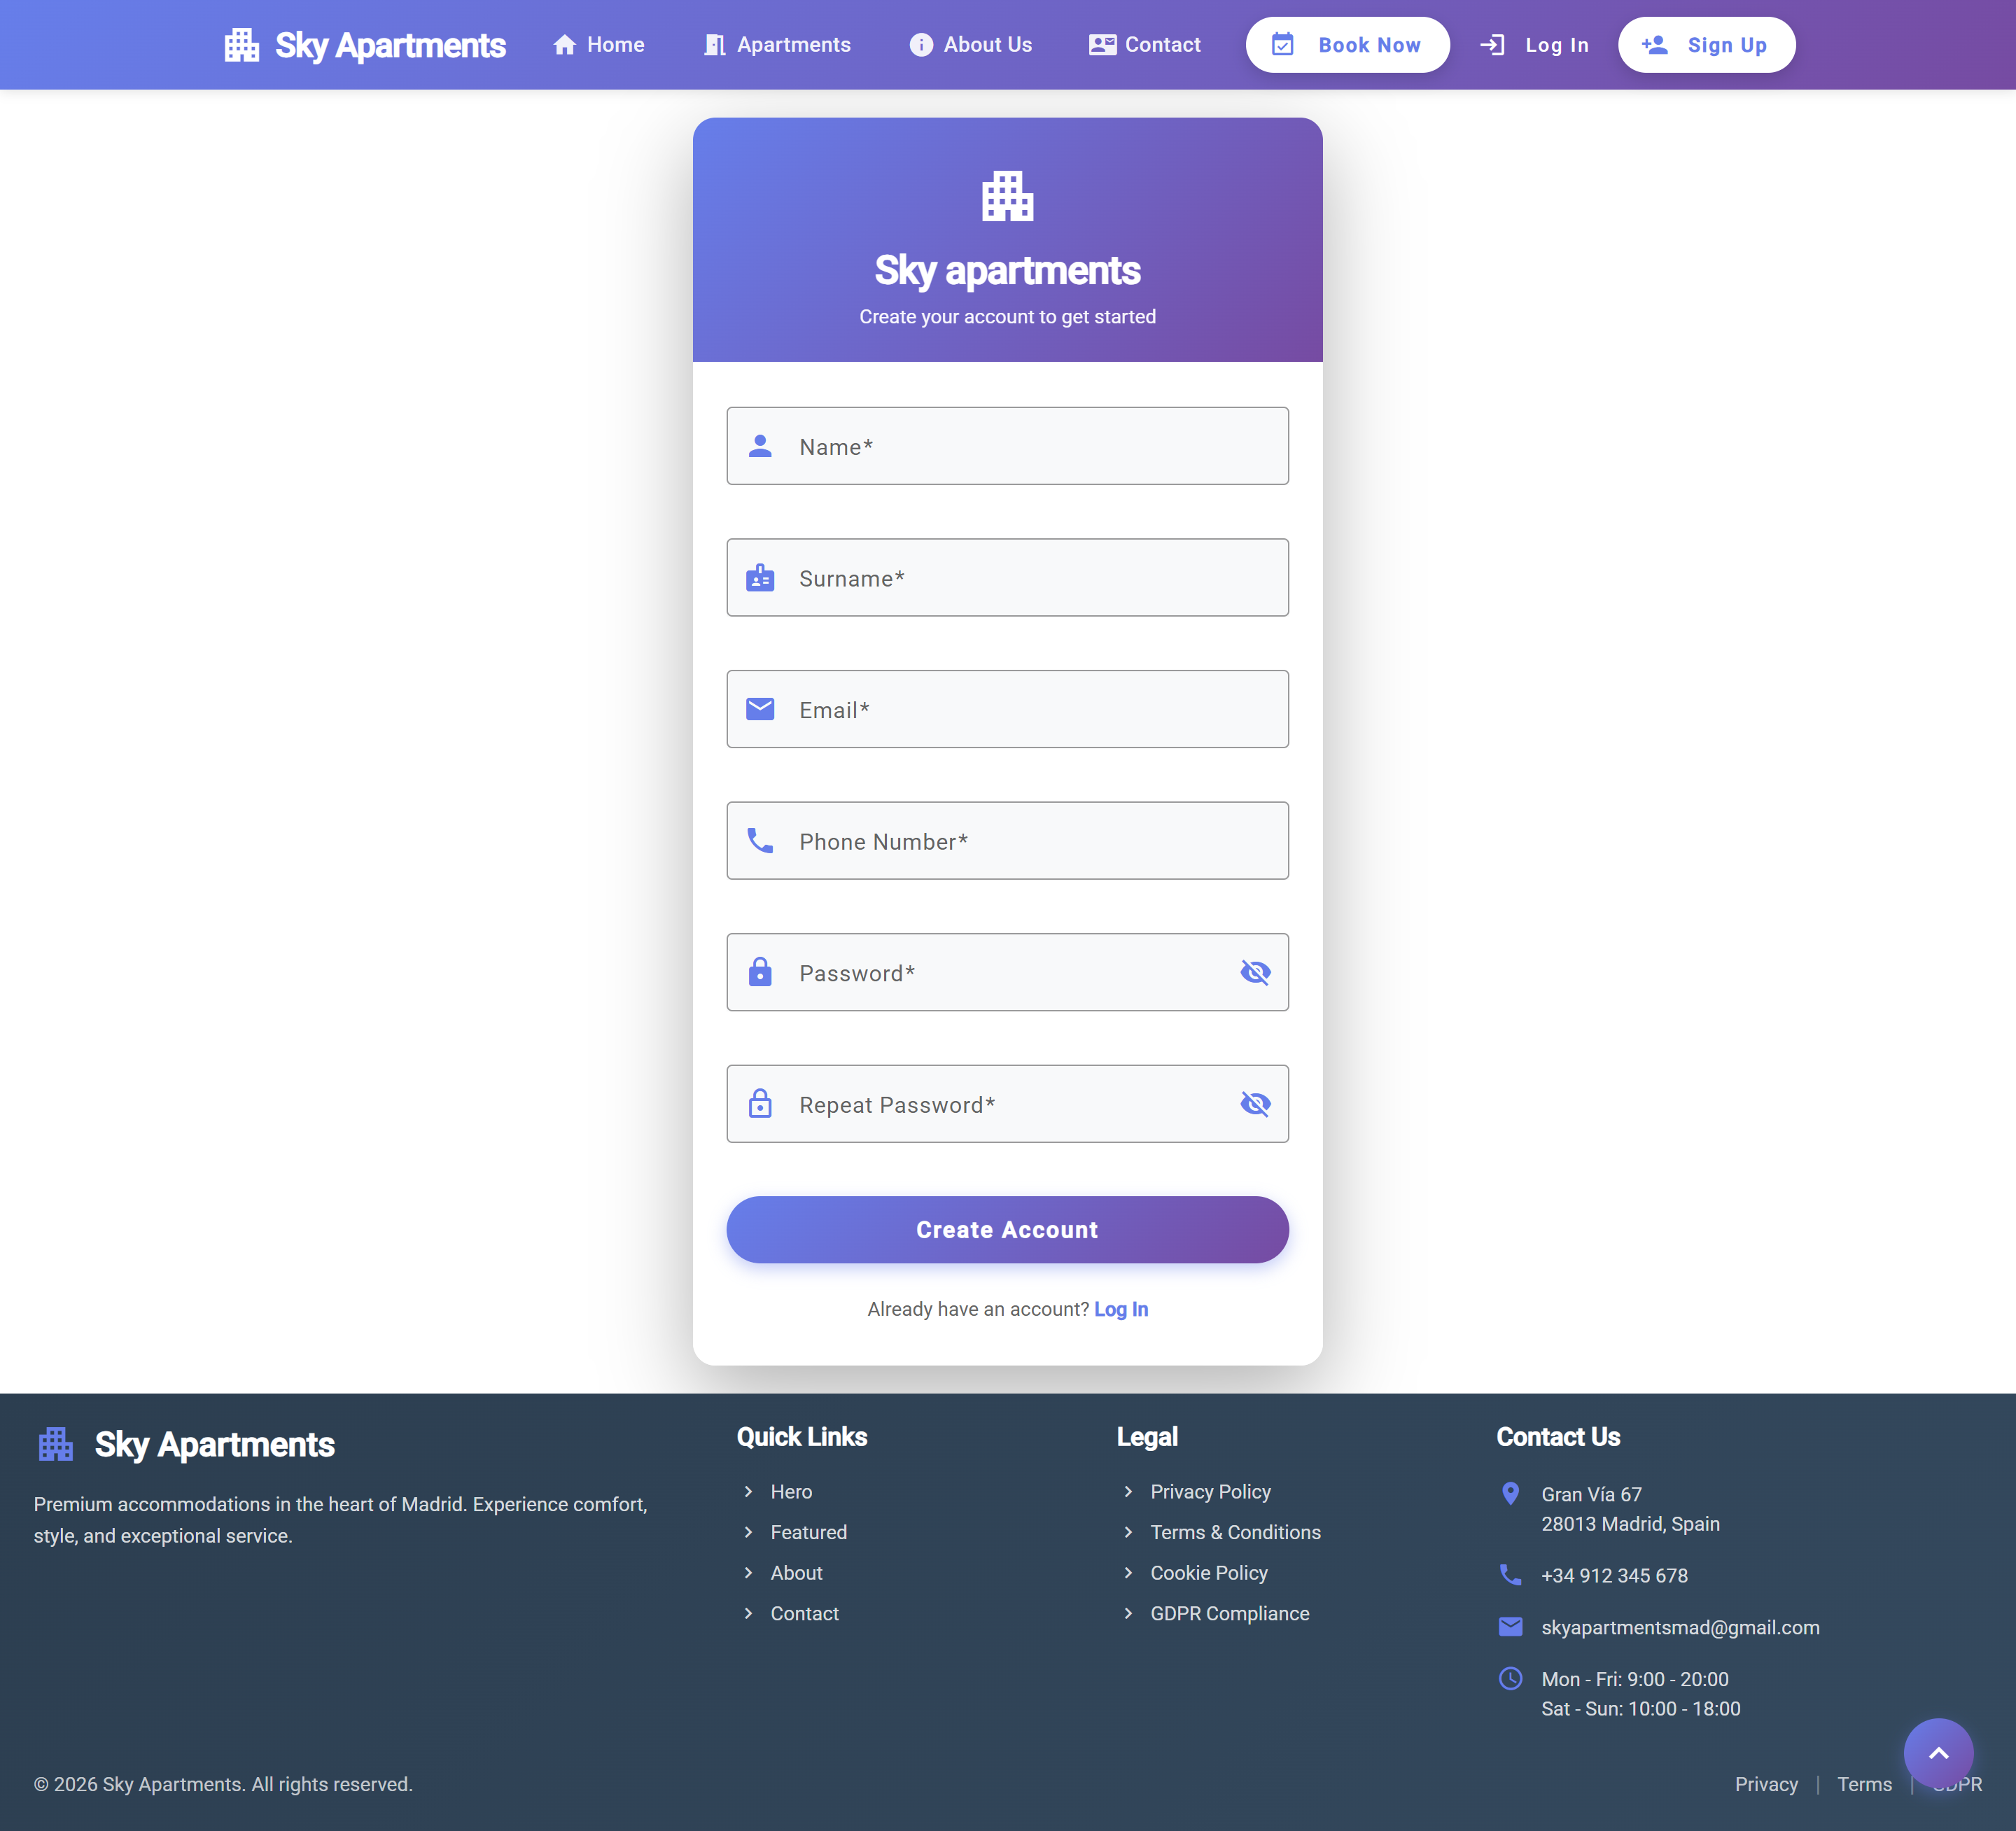
\includegraphics[width=0.8\textwidth]{img/screencapture-13-60-118-214-signup-2026-02-23-21_45_59.png}
    \caption{Formulario de registro para nuevos usuarios (Sign Up).}
\end{figure}

\begin{figure}[H]
    \centering
    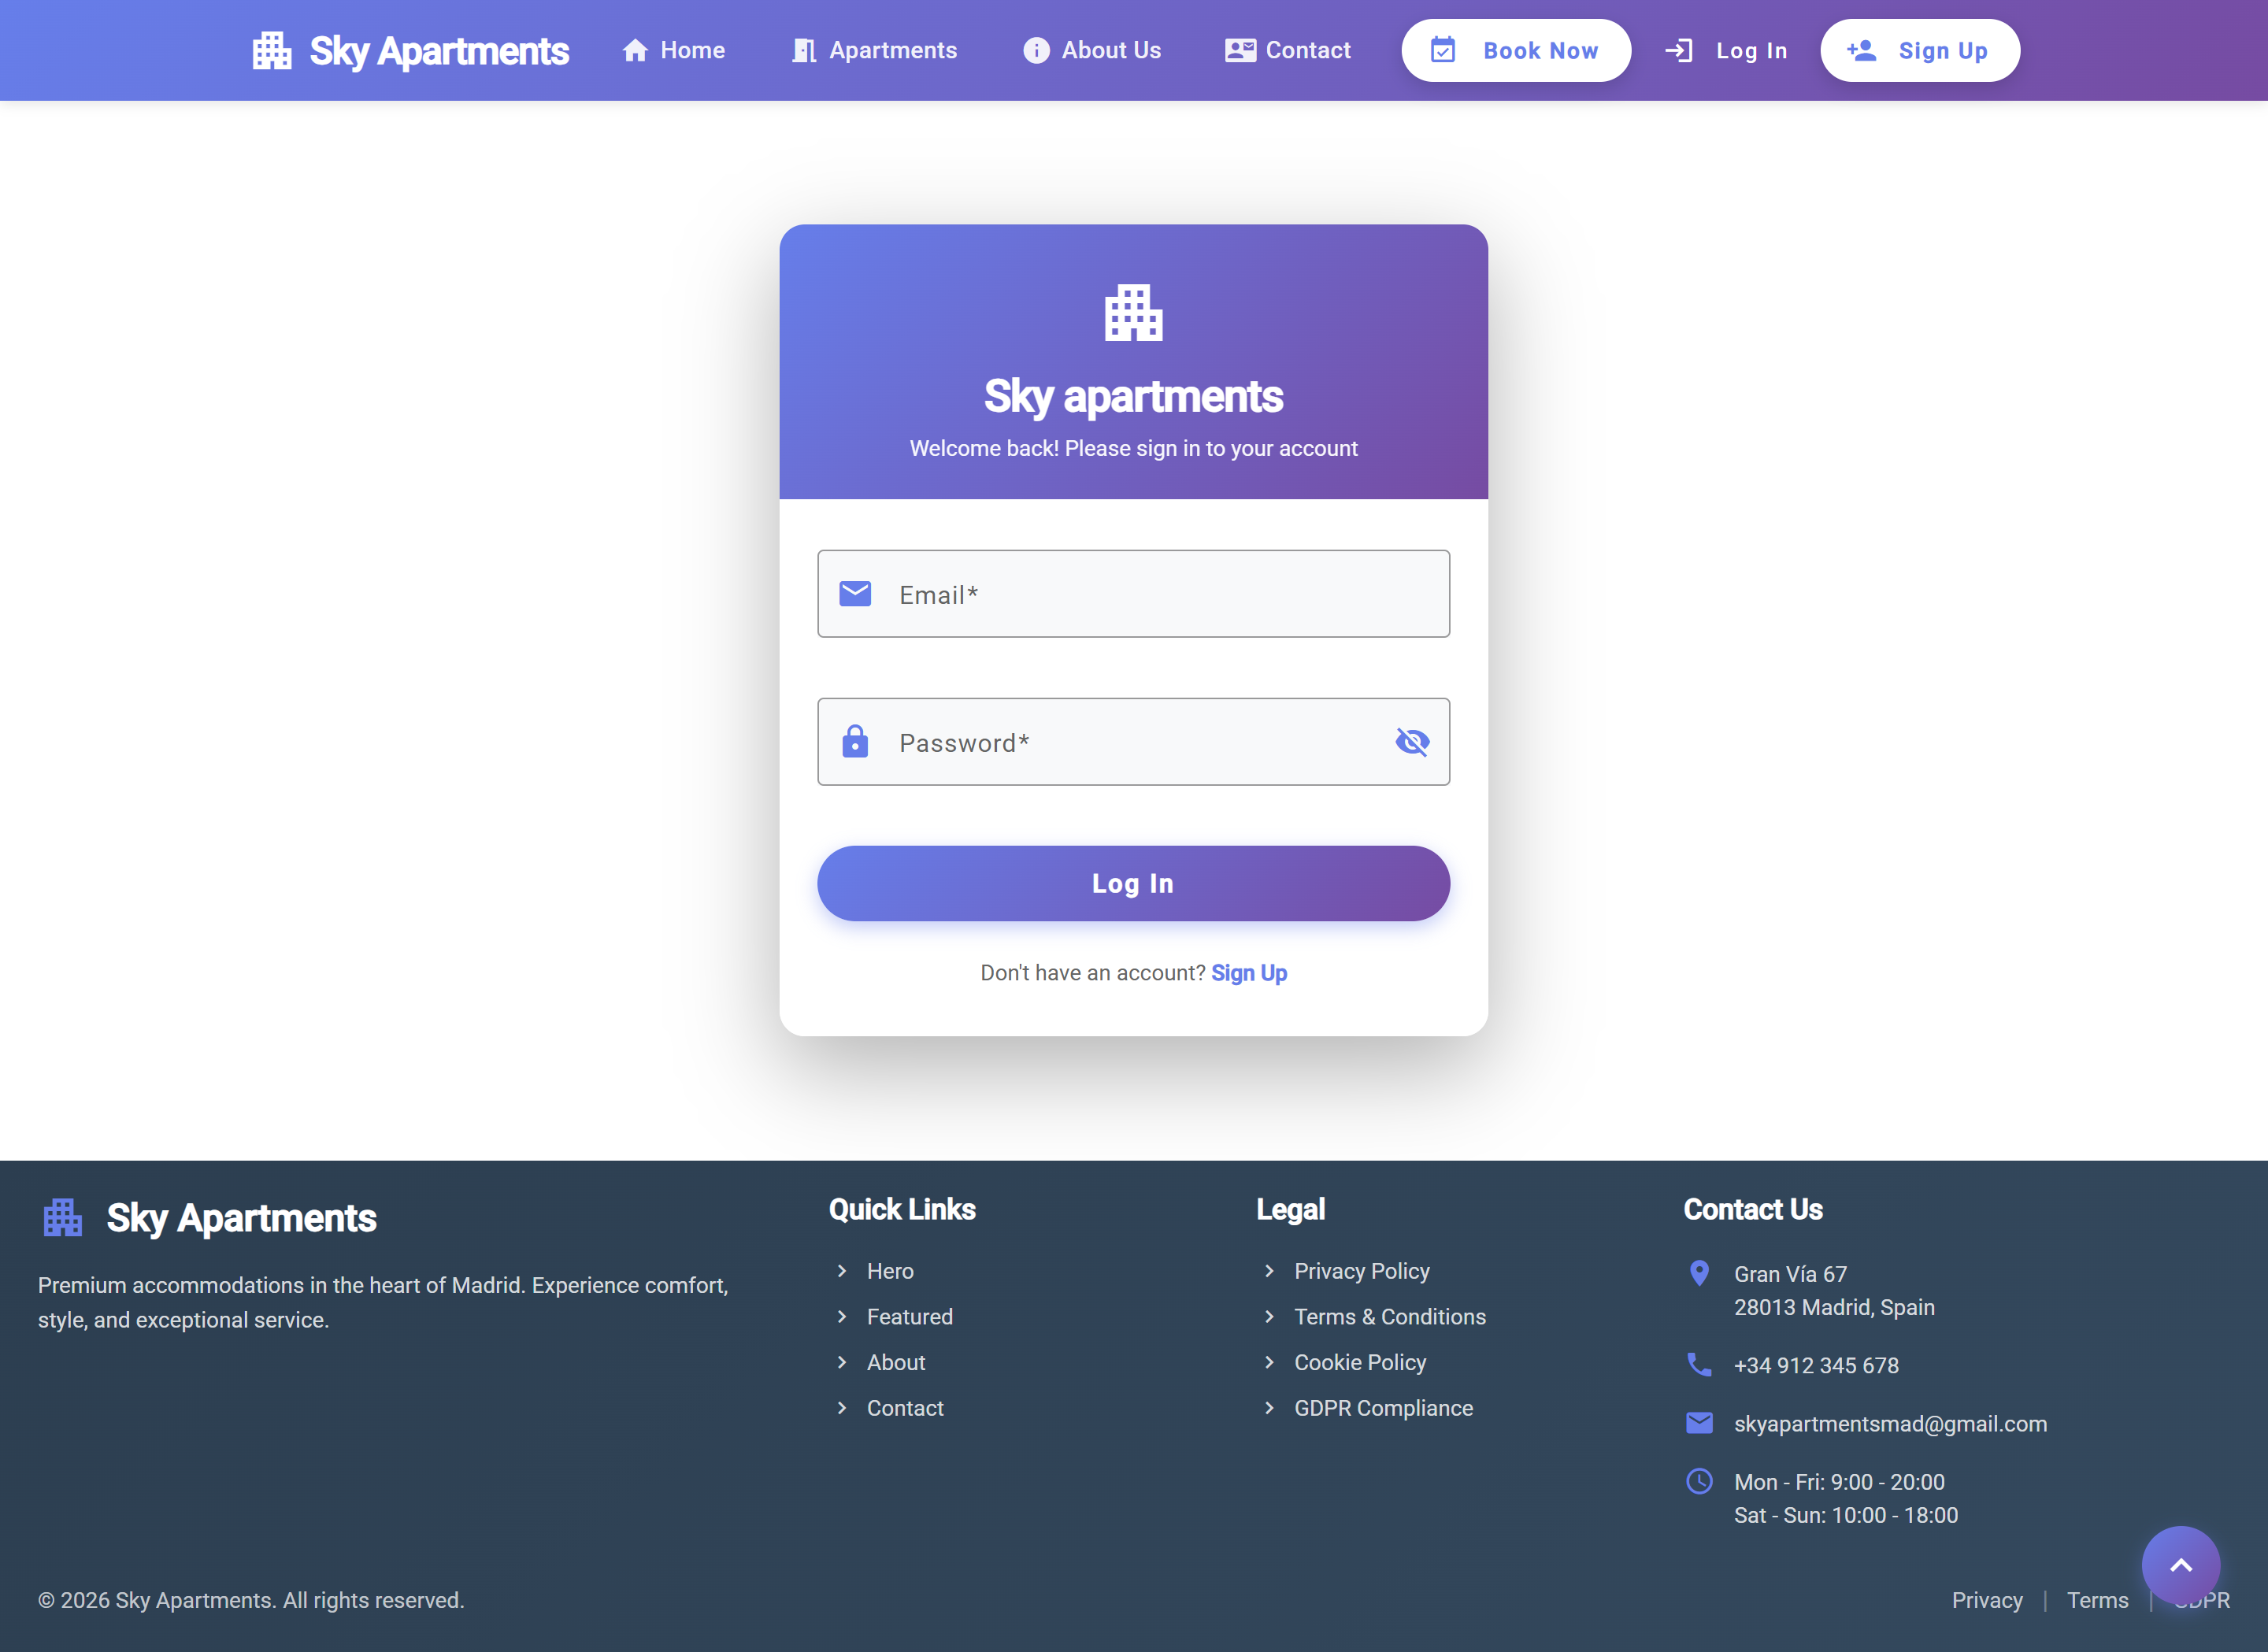
\includegraphics[width=0.8\textwidth]{img/screencapture-13-60-118-214-login-2026-02-23-21_45_52.png}
    \caption{Pantalla de inicio de sesión seguro (Log In).}
\end{figure}

\subsection{Explorando el Catálogo y Filtros}
En la sección principal de alojamientos, dispone de un buscador intuitivo en la barra lateral izquierda. Este panel permite filtrar los resultados en tiempo real basándose en sus necesidades: capacidad mínima (número de huéspedes), valoración media y comodidades requeridas (WiFi, piscina, terraza, etc.).

\begin{figure}[H]
    \centering
    \includegraphics[width=0.55\textwidth]{img/screencapture-13-60-118-214-apartments-2026-02-23-21_45_08.png}
    \caption{Catálogo de apartamentos con filtros avanzados en la barra lateral.}
\end{figure}

\subsection{Búsqueda por Fechas y Proceso de Reserva}
Si tiene unas fechas de viaje cerradas, puede hacer clic en el botón \textbf{"Book Now"}. Esto desplegará una interfaz específica donde podrá establecer las fechas exactas de \textit{Check-in} y \textit{Check-out}. El sistema calculará la disponibilidad en tiempo real y le mostrará únicamente las opciones libres.

\begin{figure}[H]
    \centering
    \includegraphics[width=0.55\textwidth]{img/screencapture-13-60-118-214-book-apartment-2026-02-23-21_45_24.png}
    \caption{Interfaz de selección de fechas para comprobar disponibilidad y calcular precios.}
\end{figure}

\subsection{Detalle del Apartamento y Reseñas}
Al seleccionar un alojamiento, accederá a su página de detalle. Aquí podrá explorar una galería interactiva de imágenes, leer la descripción y utilizar el widget lateral para confirmar la reserva. En la parte inferior, podrá leer las reseñas (de 1 a 5 estrellas) dejadas por huéspedes anteriores, así como escribir la suya propia tras finalizar su estancia.

\begin{figure}[H]
    \centering
    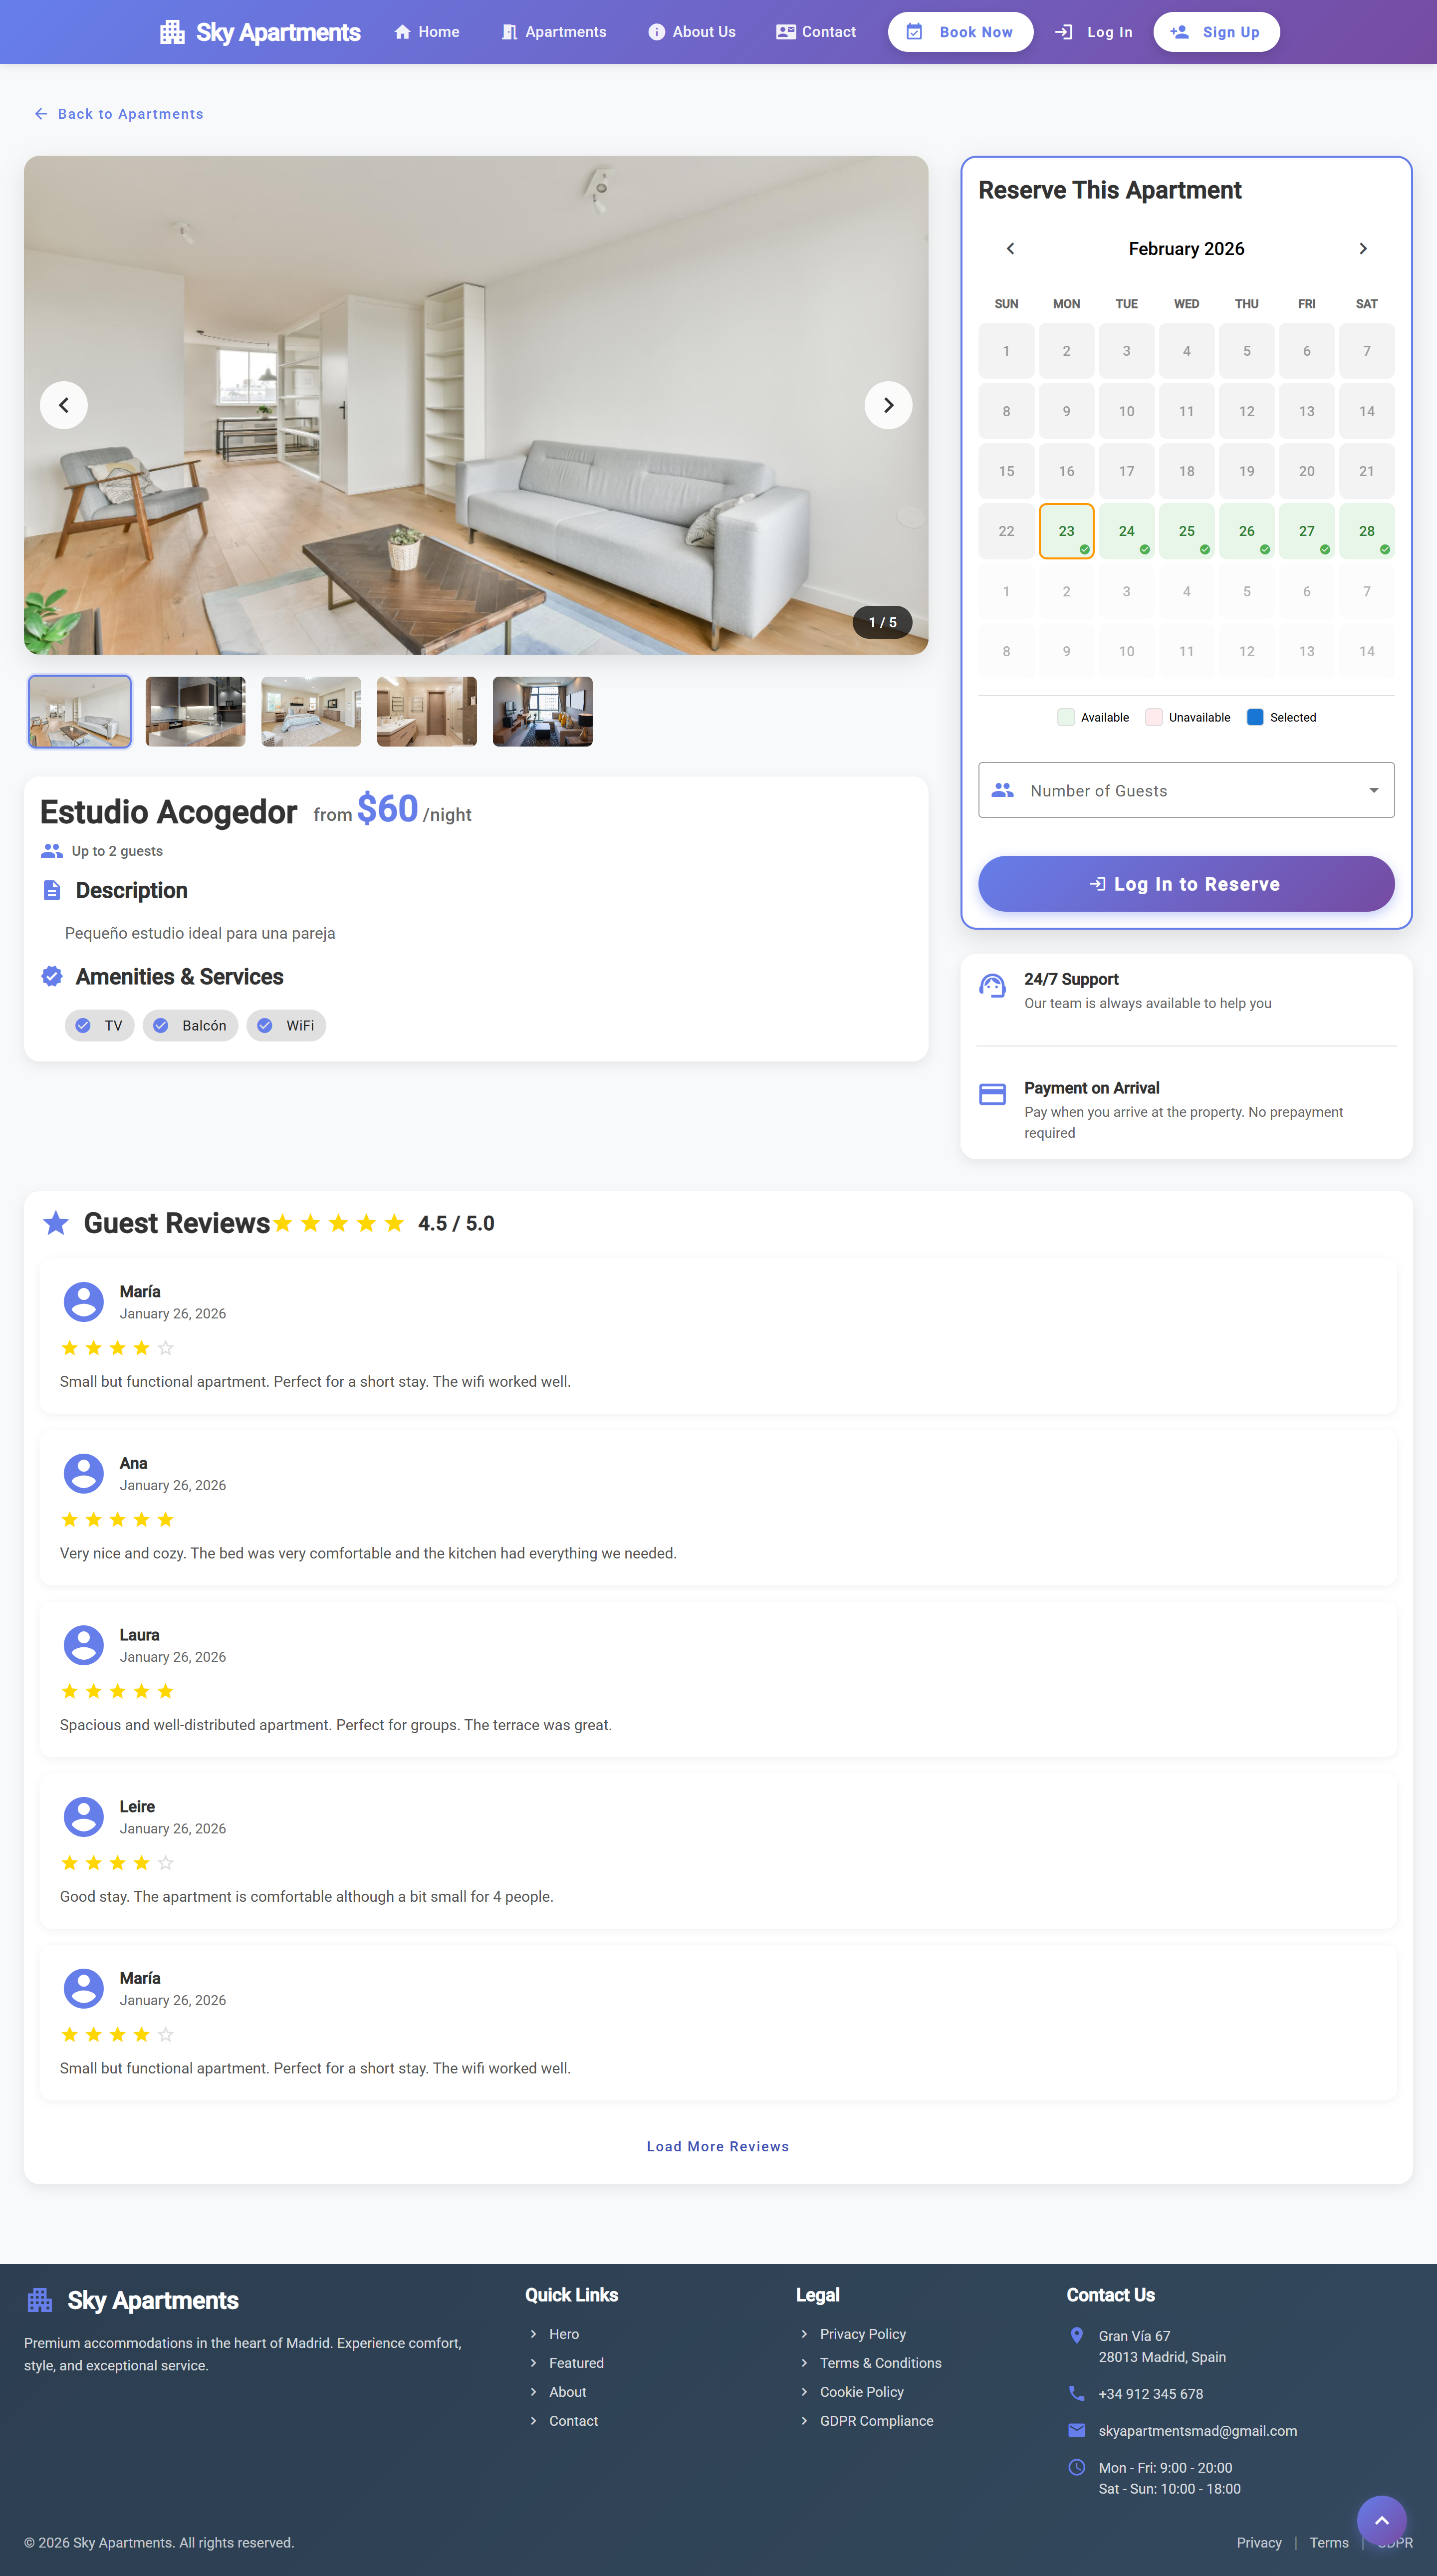
\includegraphics[width=0.8\textwidth]{img/screencapture-13-60-118-214-apartment-3-2026-02-23-21_45_42.png}
    \caption{Vista detallada de un apartamento, calendario de reservas y sistema de reseñas.}
\end{figure}

\subsection{Gestión de la Cuenta y Perfil Personal}
Haciendo clic en el icono de sus iniciales (esquina superior derecha), accederá a su área personal. En la pestaña \textbf{"Personal Information"} podrá consultar y actualizar sus datos de contacto en cualquier momento, así como modificar su contraseña de acceso.

\begin{figure}[H]
    \centering
    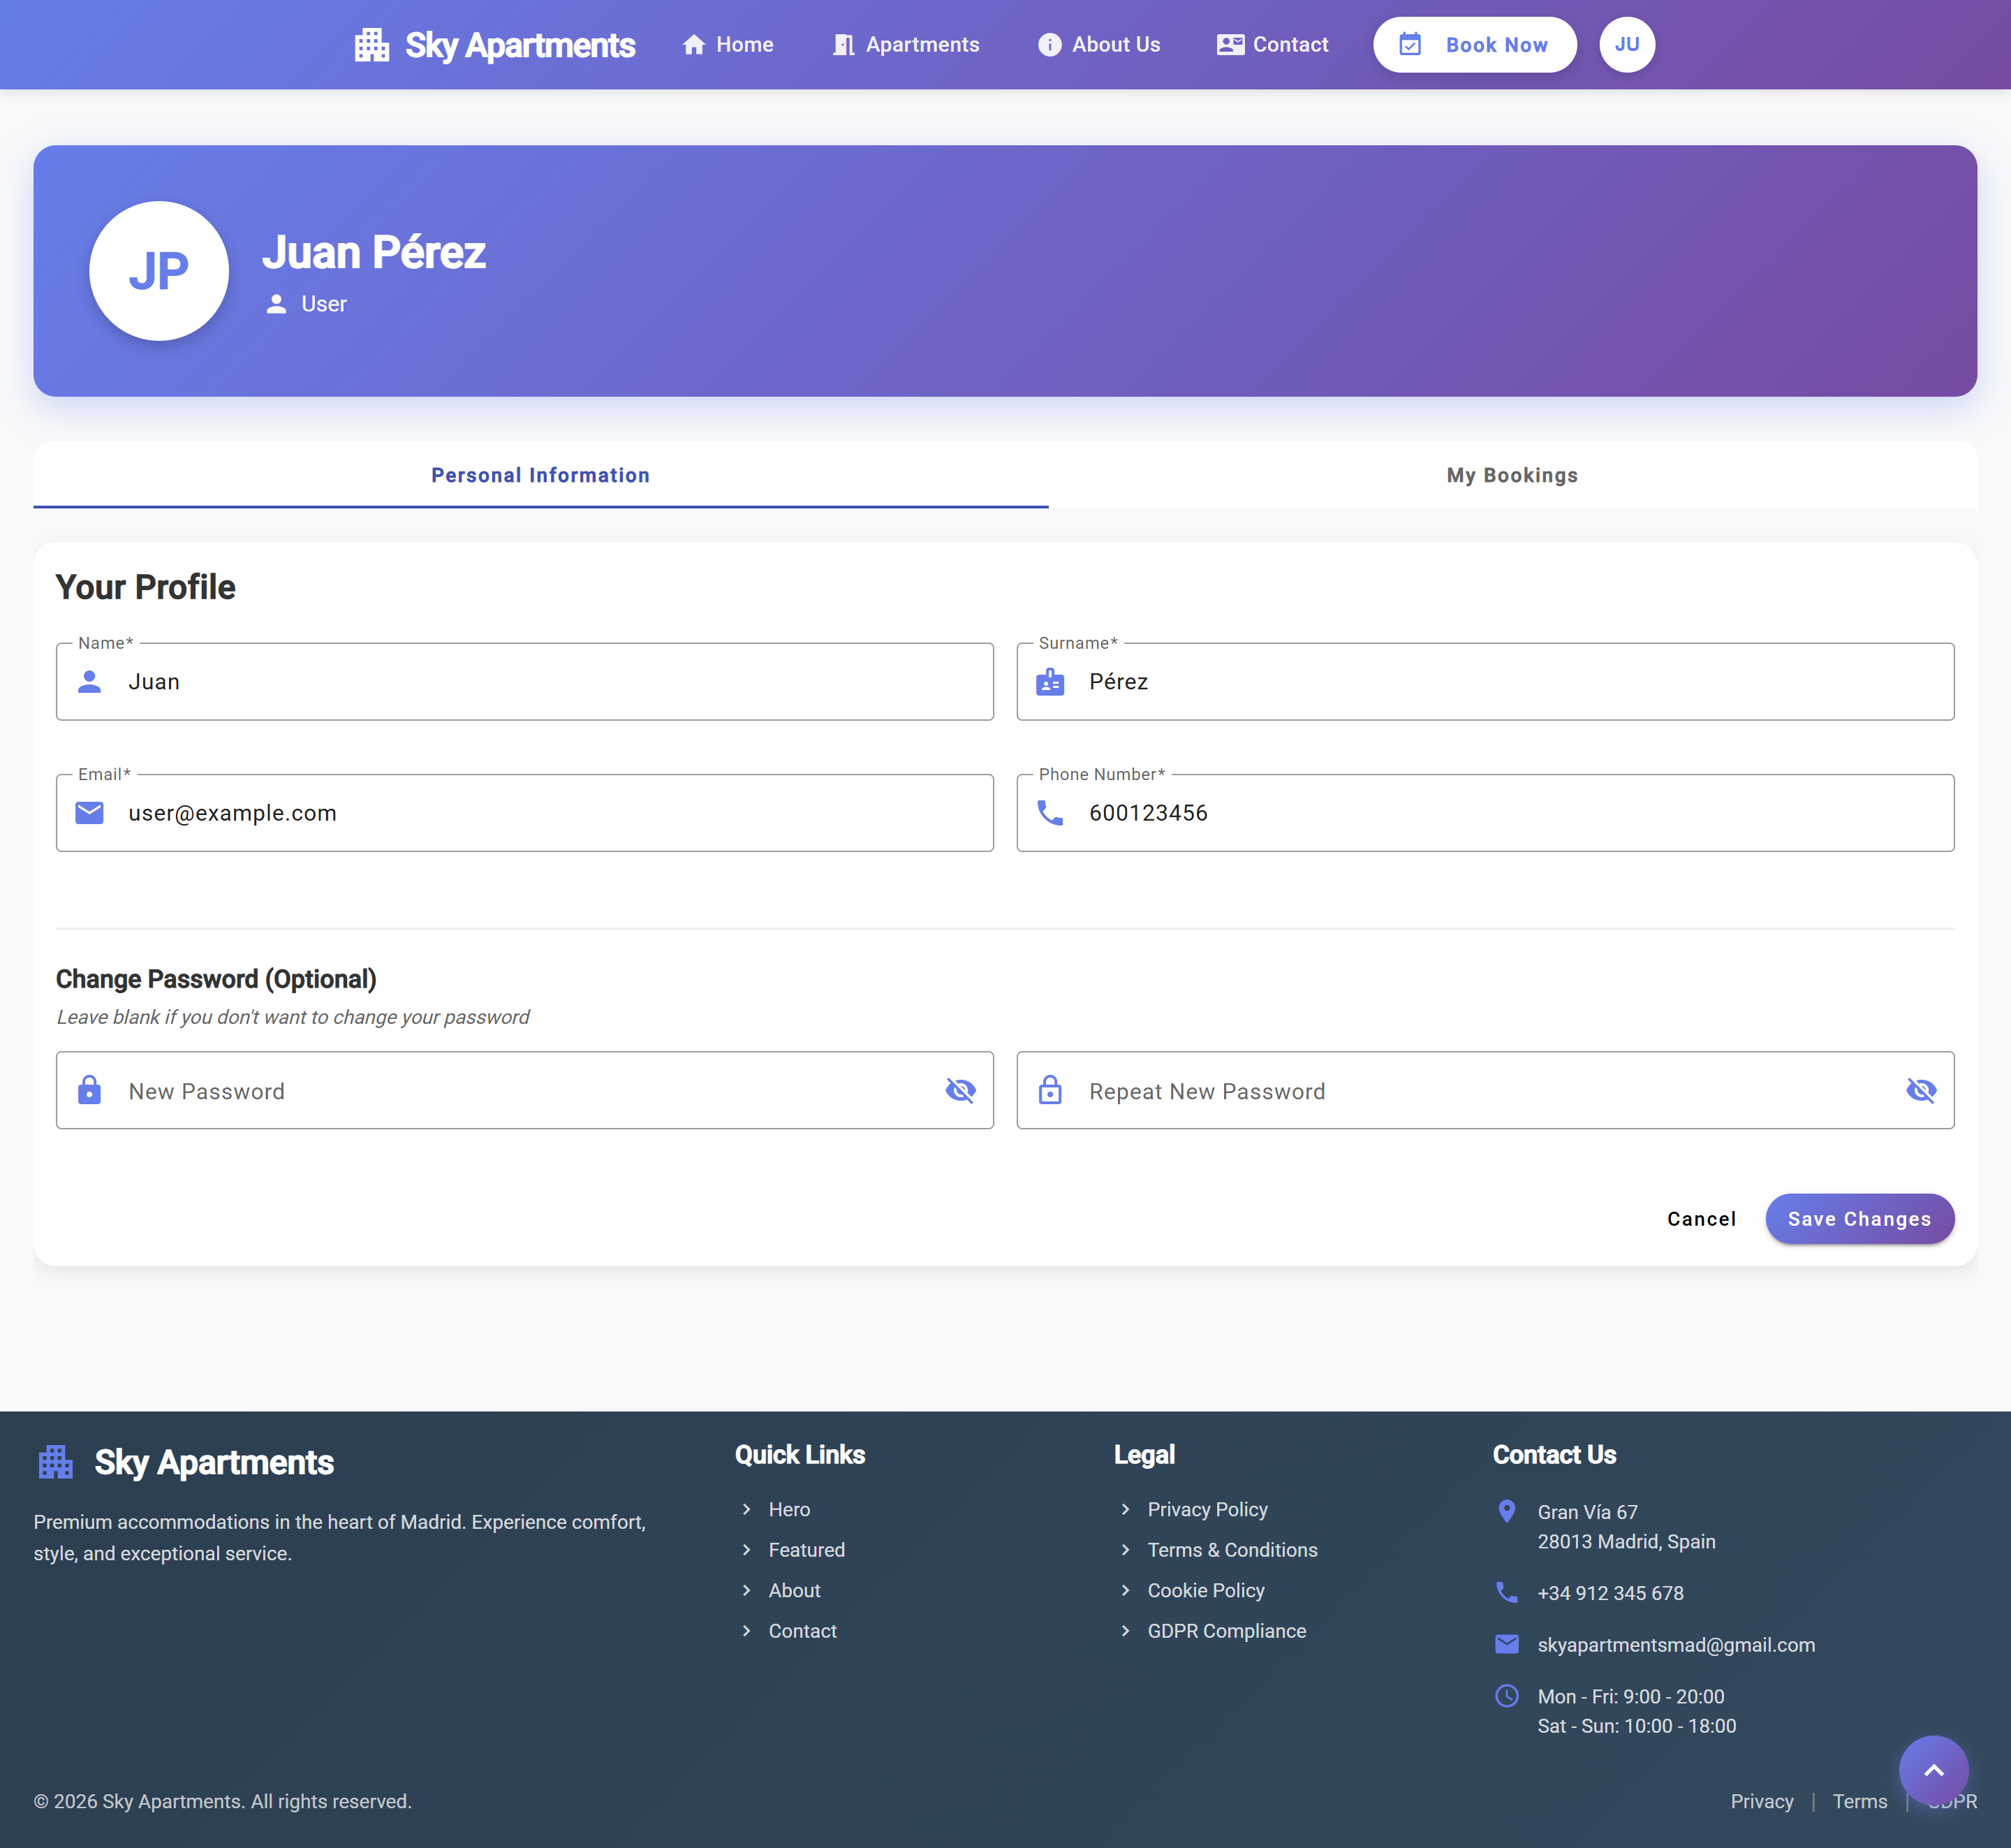
\includegraphics[width=0.8\textwidth]{img/screencapture-13-60-118-214-profile-2026-02-23-21_46_26.png}
    \caption{Área de gestión de datos personales del perfil de usuario.}
\end{figure}

En la pestaña \textbf{"My Bookings"} (Mis Reservas), podrá consultar su historial completo, ver el estado de cada estancia (confirmada, completada, cancelada) y cancelar activamente aquellas reservas que aún no hayan comenzado.

\begin{figure}[H]
    \centering
    \includegraphics[width=0.6\textwidth]{img/screencapture-13-60-118-214-profile-2026-02-23-21_46_40.png}
    \caption{Historial de reservas del usuario y gestión de cancelaciones.}
\end{figure}


\section{Guía de Administración (Panel Privado)}
Los usuarios con el rol de Administrador tienen acceso a un panel de control avanzado desde donde pueden gestionar integralmente el negocio.

\subsection{Dashboard Analítico}
Al entrar al panel, la pestaña \textbf{"Dashboard"} ofrece una visión panorámica del rendimiento. Incluye métricas clave como los ingresos totales generados, una gráfica de la ocupación en el tiempo y ránkings automáticos de los apartamentos más reservados y los mejor valorados. Esta información se puede filtrar por períodos específicos para analizar tendencias estacionales o el impacto de promociones.

\begin{figure}[H]
    \centering
    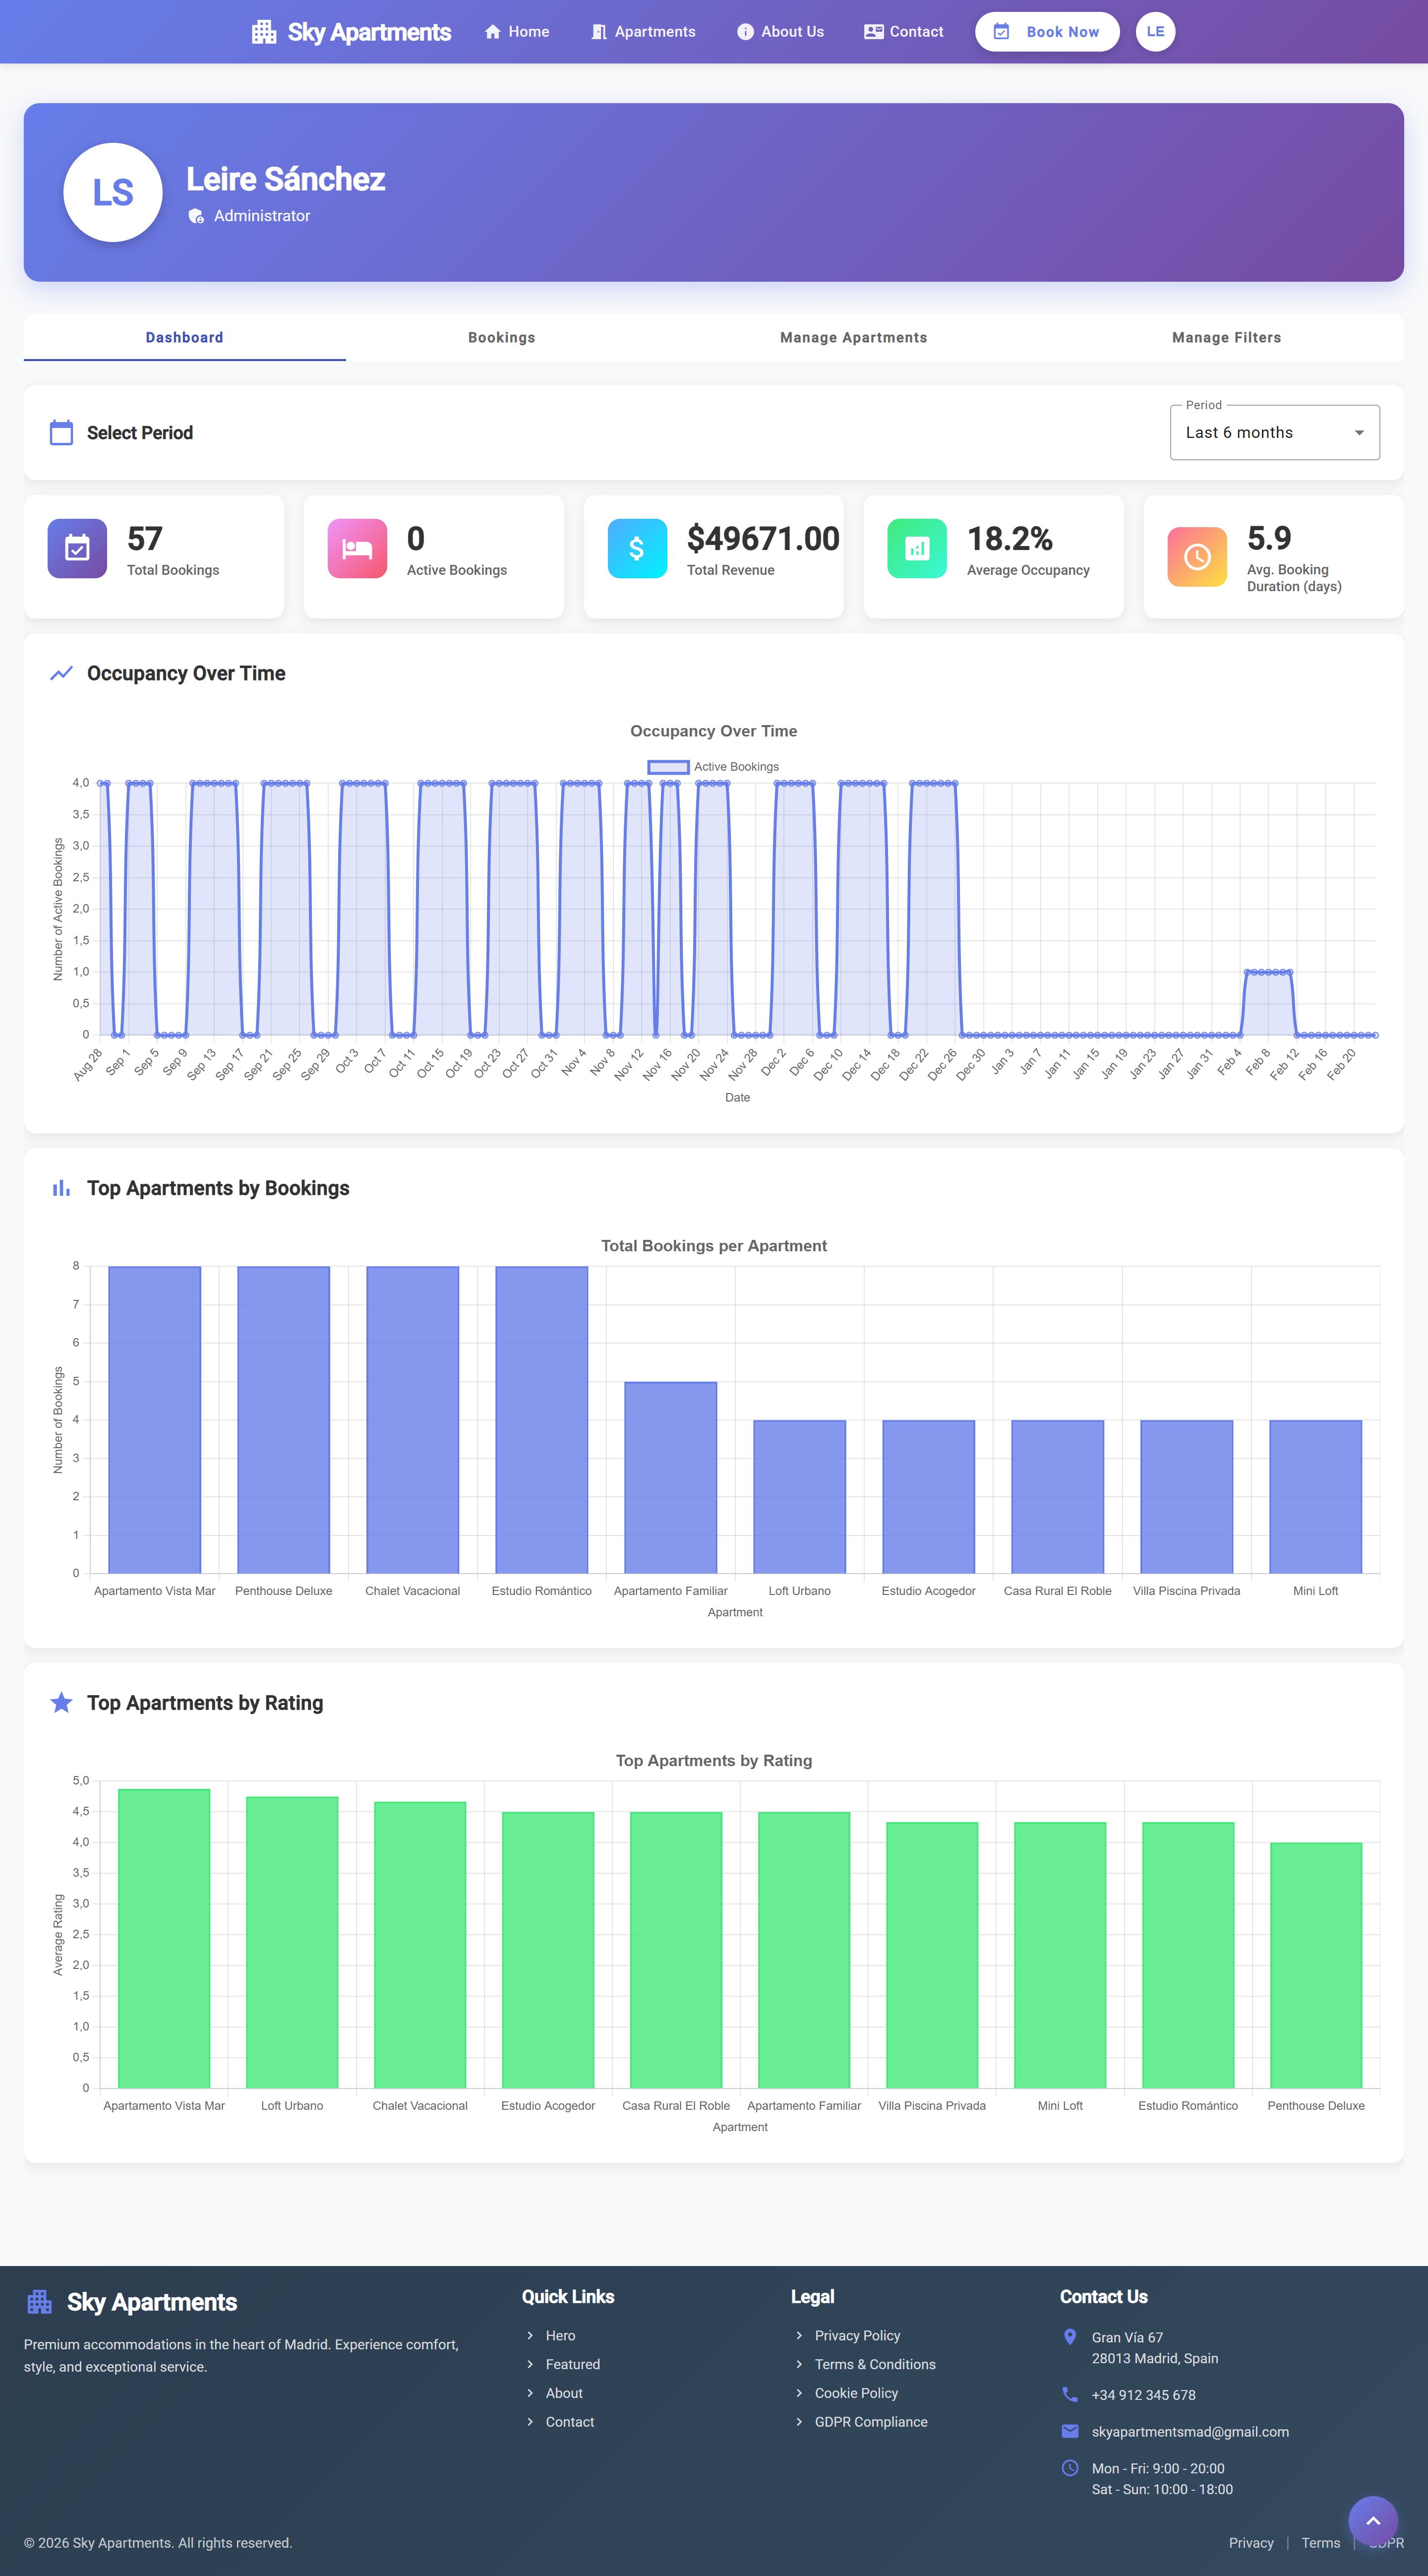
\includegraphics[width=0.8\textwidth]{img/screencapture-13-60-118-214-profile-2026-02-23-21_47_11.png}
    \caption{Dashboard principal de administración con métricas y gráficas de rendimiento.}
\end{figure}

\subsection{Gestión Global de Reservas}
La pestaña \textbf{"Bookings"} permite al administrador supervisar toda la actividad. Ofrece una vista visual de calendario o formato lista, e incorpora un buscador y un filtro por estado para encontrar rápidamente reservas concretas, facilitando la gestión operativa.

\begin{figure}[H]
    \centering
    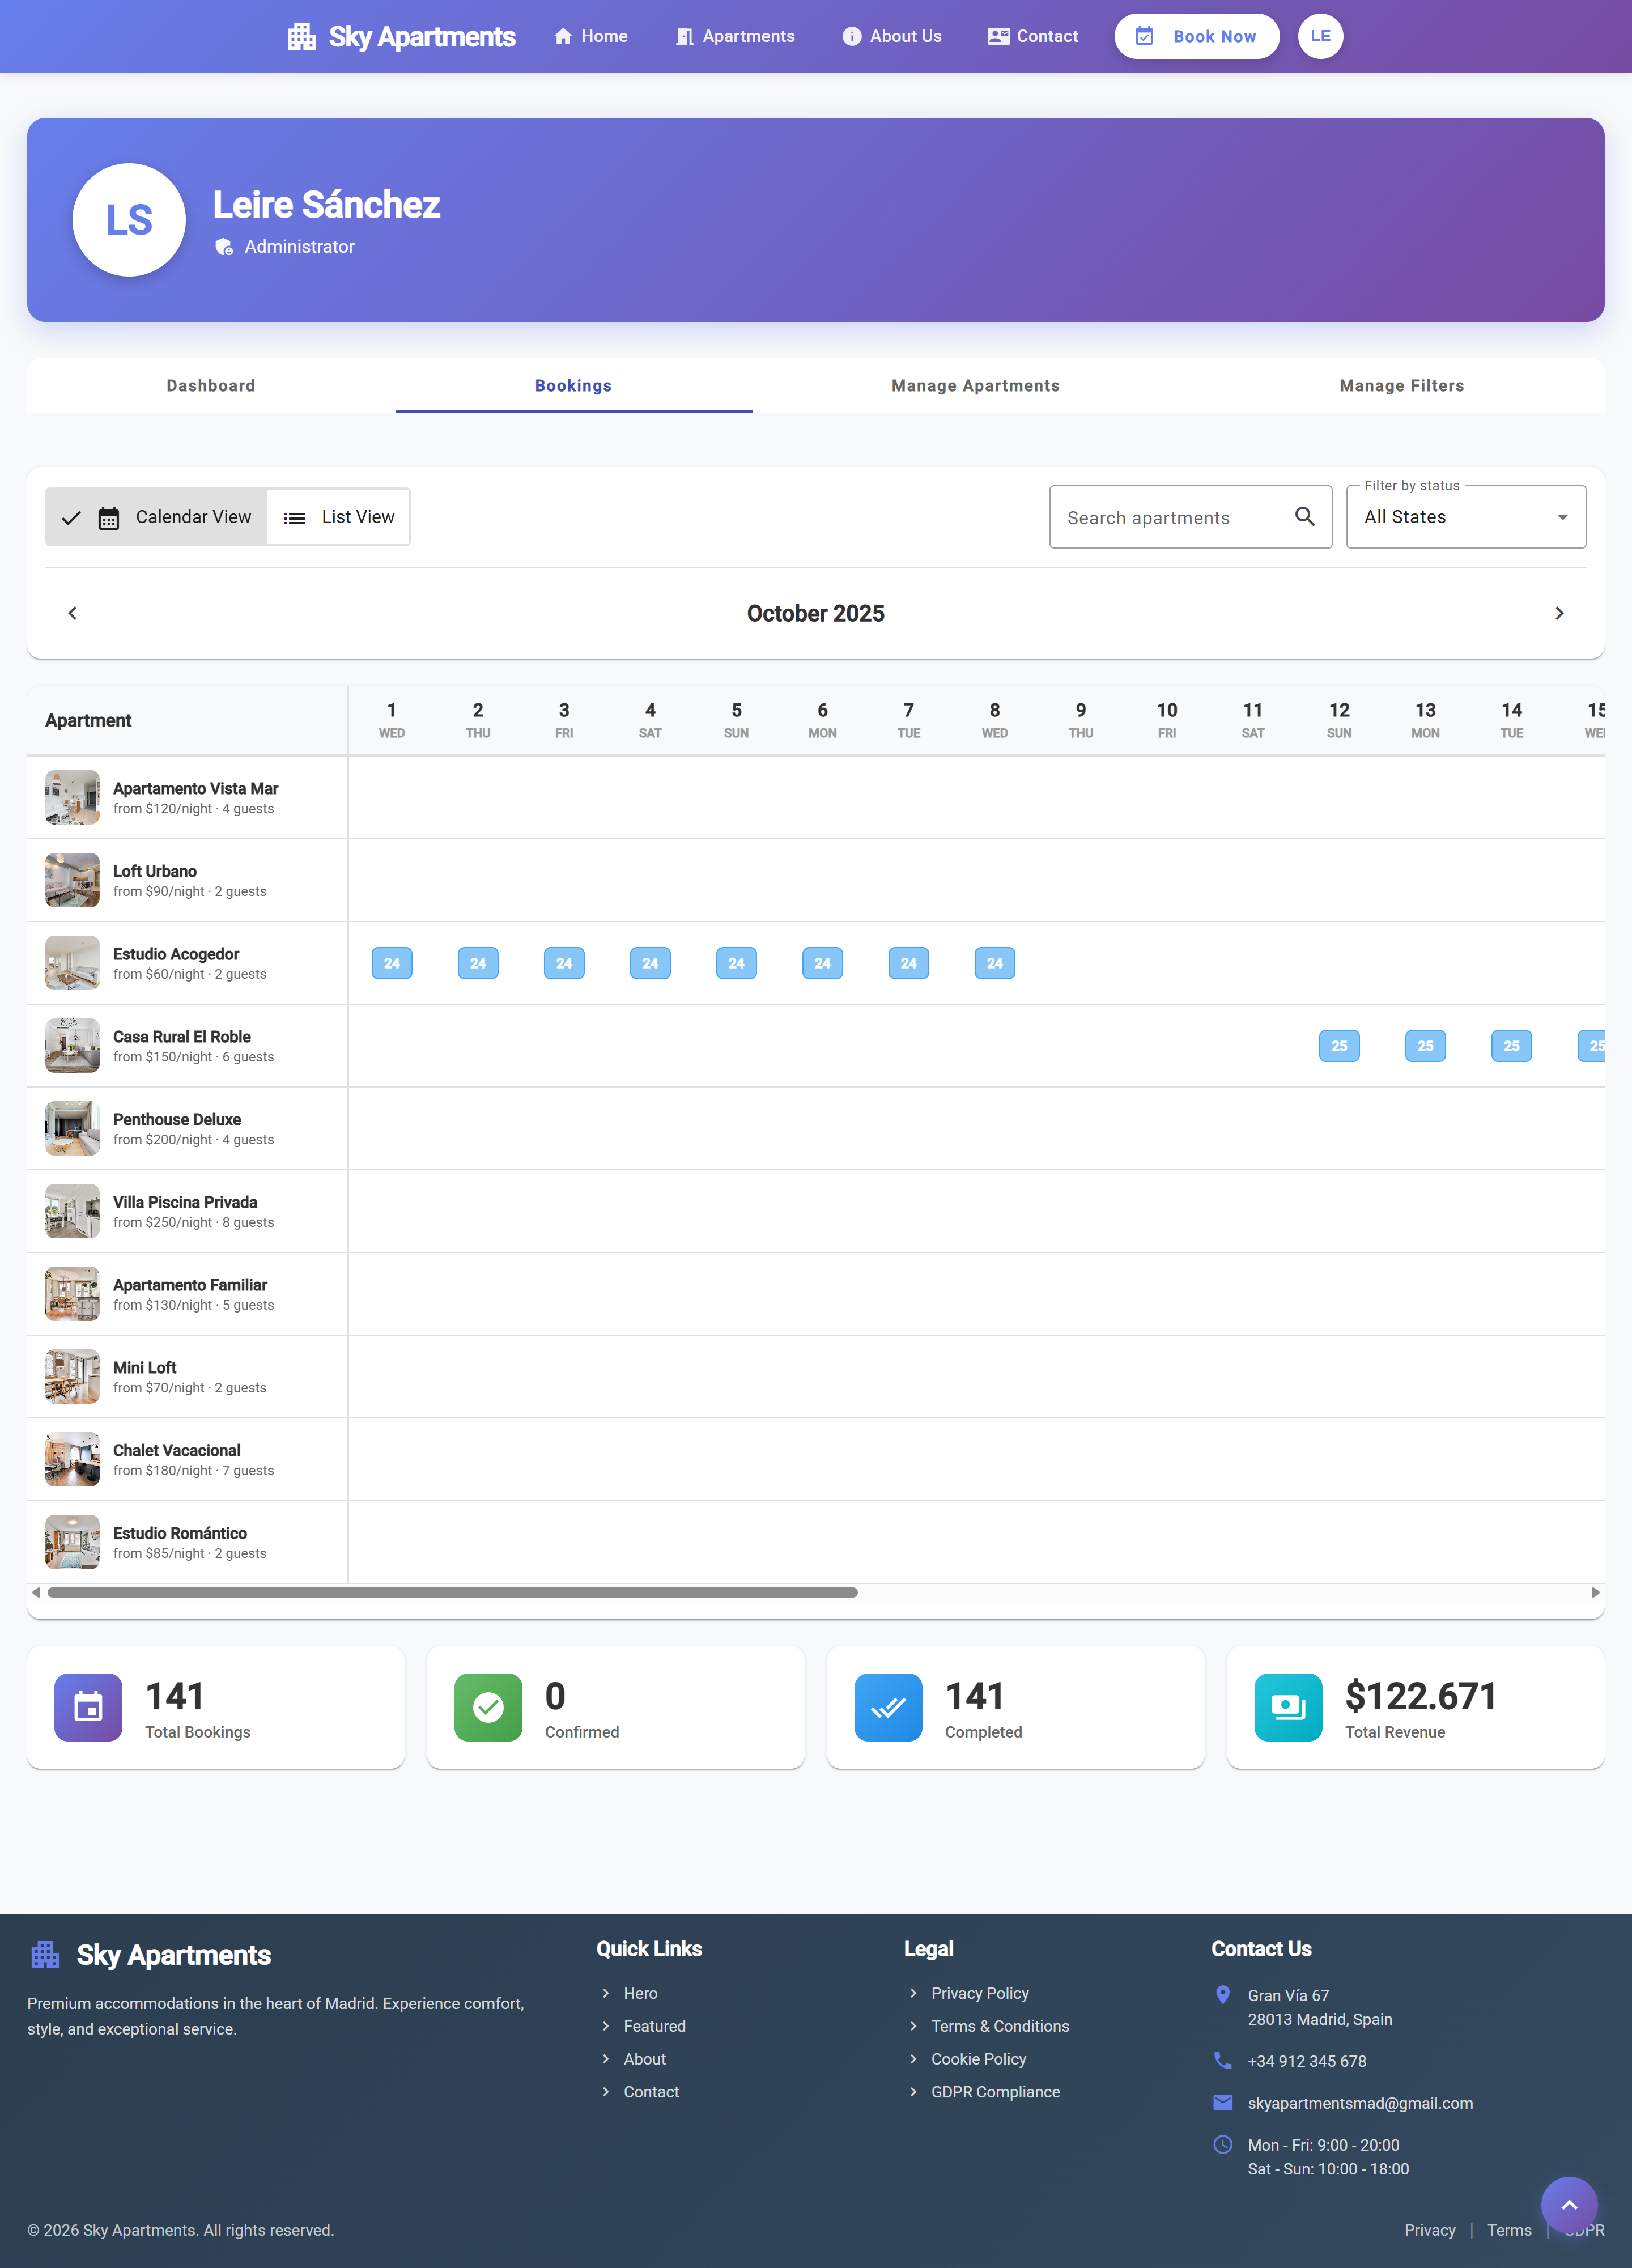
\includegraphics[width=0.8\textwidth]{img/screencapture-13-60-118-214-profile-2026-02-23-21_47_49.png}
    \caption{Panel de gestión y visualización de todas las reservas del sistema.}
\end{figure}

\subsection{Gestión del Catálogo de Apartamentos}
Desde la pestaña \textbf{"Manage Apartments"}, el administrador tiene una vista global de todos los alojamientos activos en el sistema, pudiendo editarlos o darlos de baja directamente desde sus respectivas tarjetas.

\begin{figure}[H]
    \centering
    \includegraphics[width=0.8\textwidth]{img/screencapture-13-60-118-214-profile-2026-02-23-21_48_01.png}
    \caption{Vista general del catálogo de alojamientos desde el panel de administración.}
\end{figure}

Haciendo clic en "Add Apartment", se abre un formulario para introducir todos los detalles de una nueva propiedad (nombre, capacidad, precio base, servicios) y subir de forma simultánea múltiples imágenes que conformarán su galería pública.

\begin{figure}[H]
    \centering
    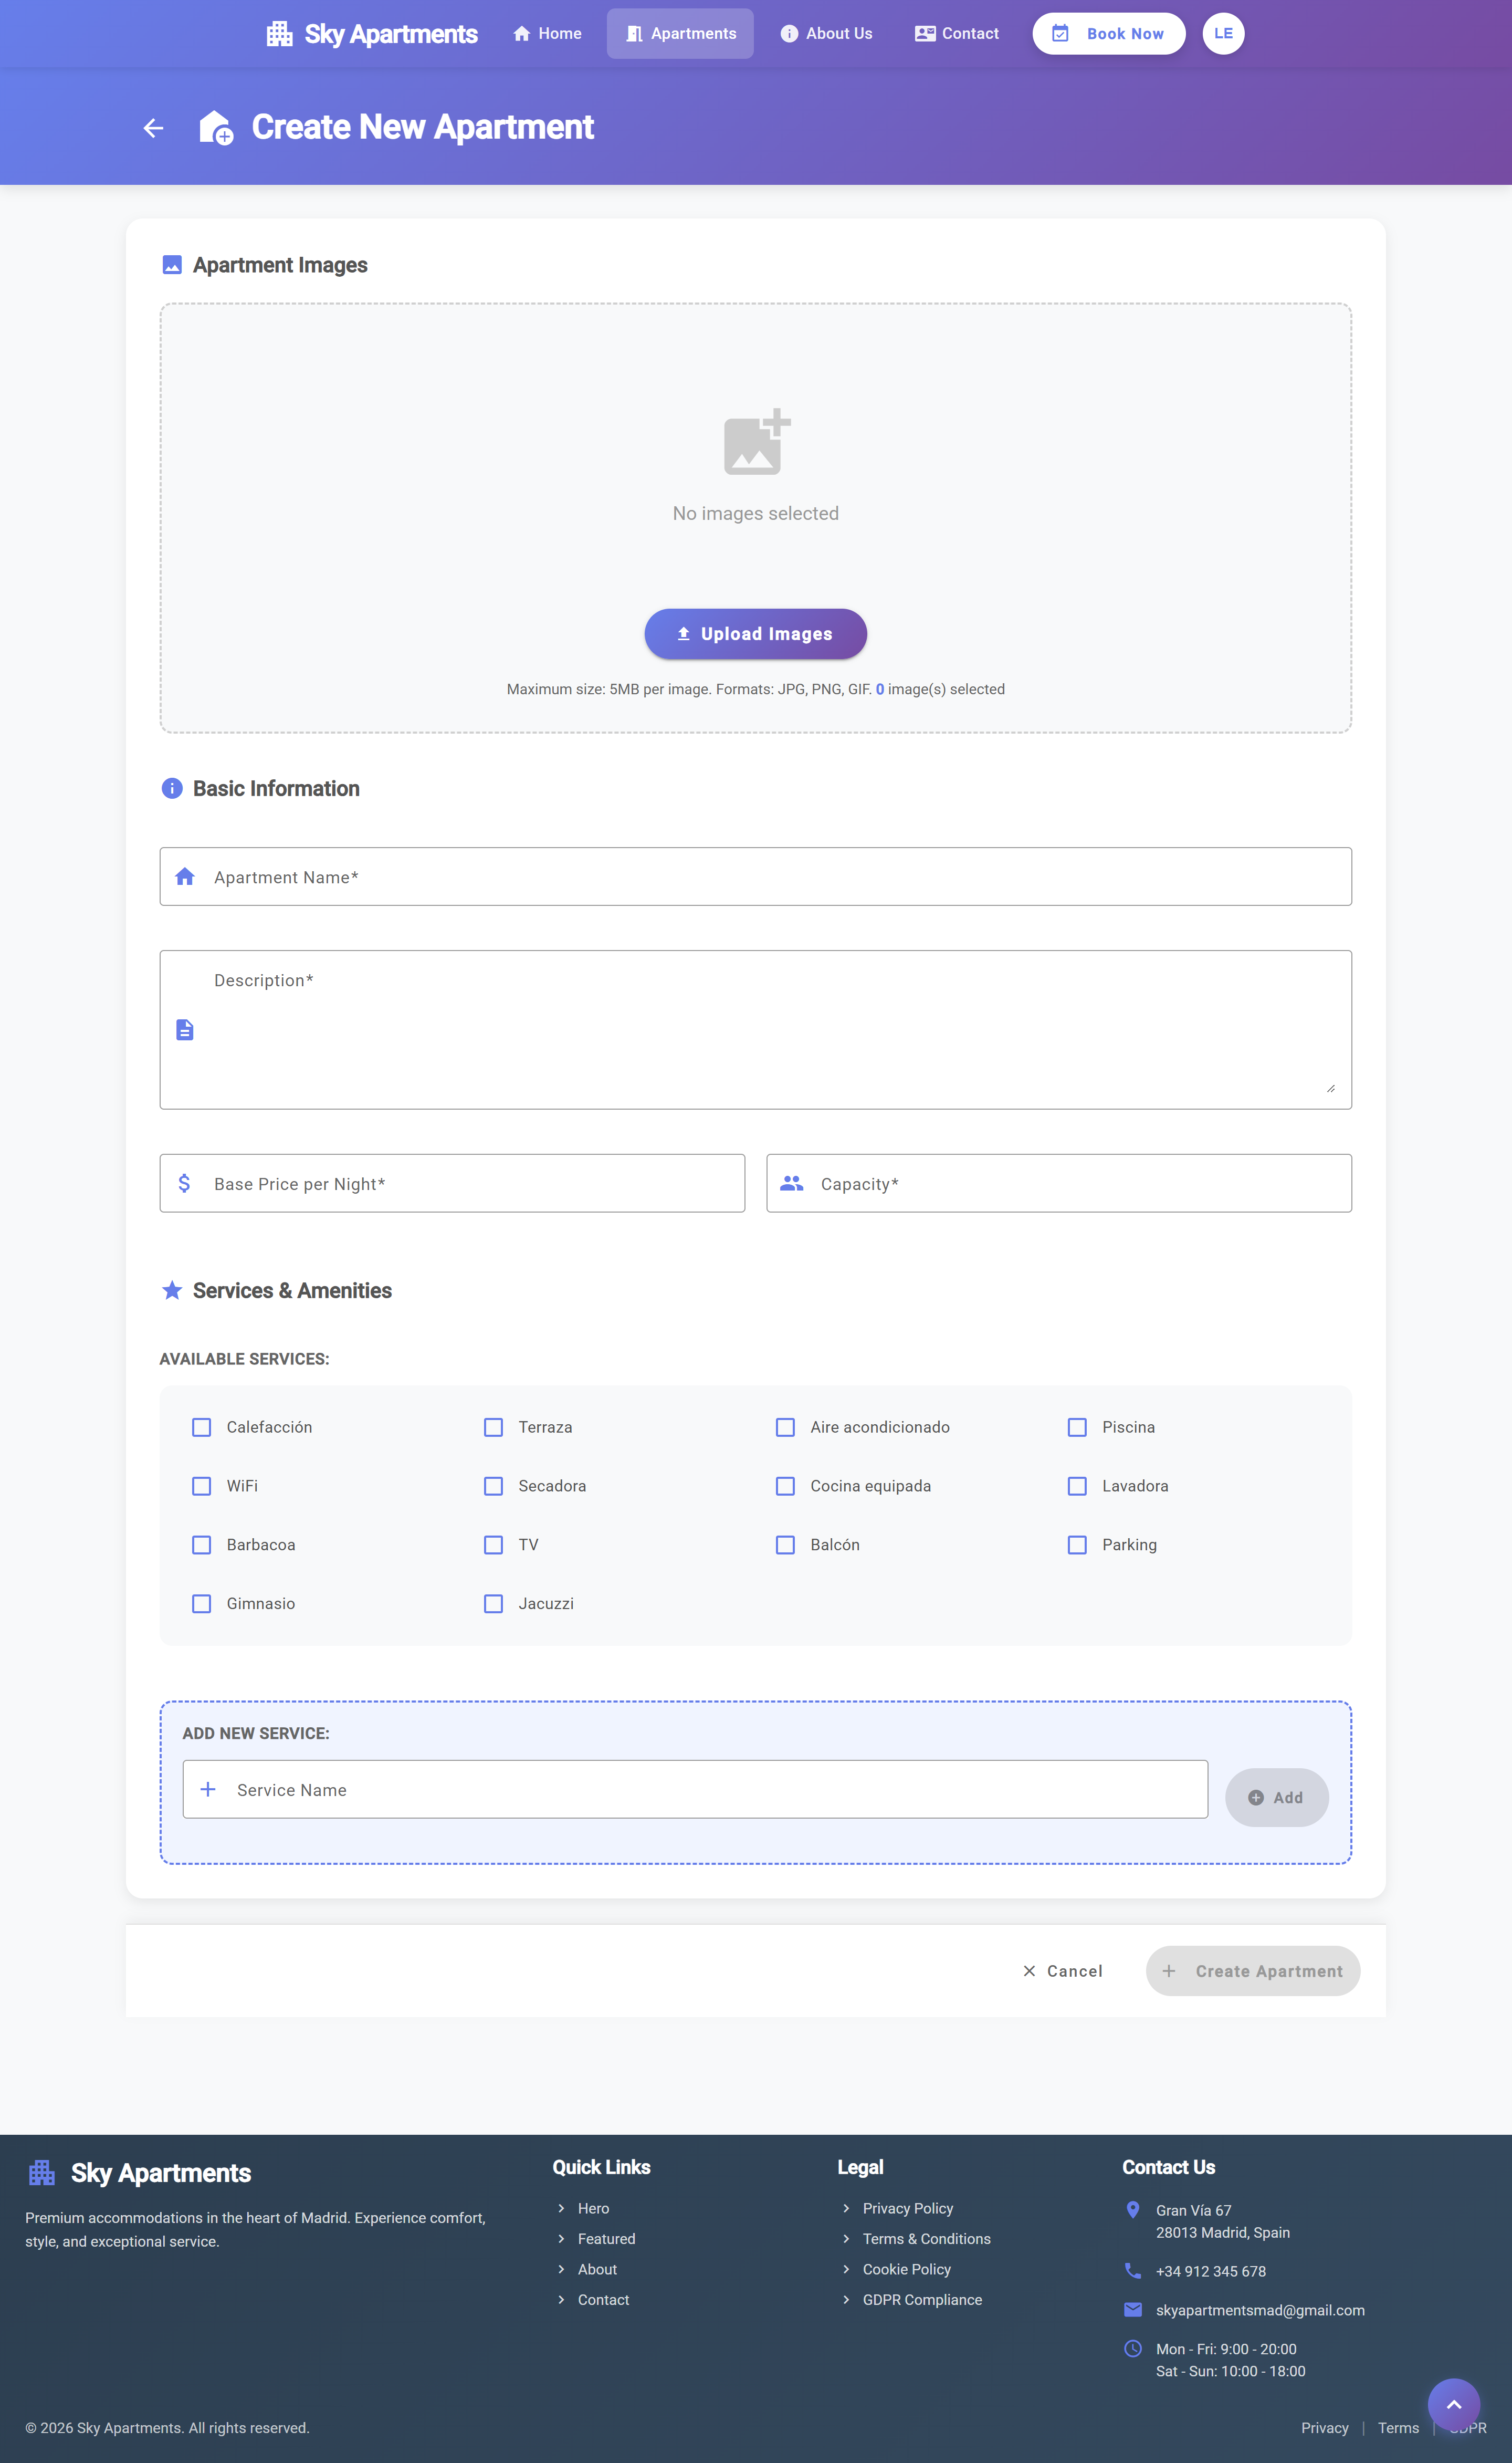
\includegraphics[width=0.8\textwidth]{img/screencapture-13-60-118-214-apartments-new-2026-02-23-21_48_14.png}
    \caption{Formulario de alta de un nuevo apartamento y subida de imágenes.}
\end{figure}

\subsection{Configuración de Precios Dinámicos (Filtros)}
La pestaña \textbf{"Manage Filters"} es el núcleo de la estrategia de ingresos. Aquí, el administrador puede visualizar, editar o eliminar todas las reglas de precio activas en la plataforma.

\begin{figure}[H]
    \centering
    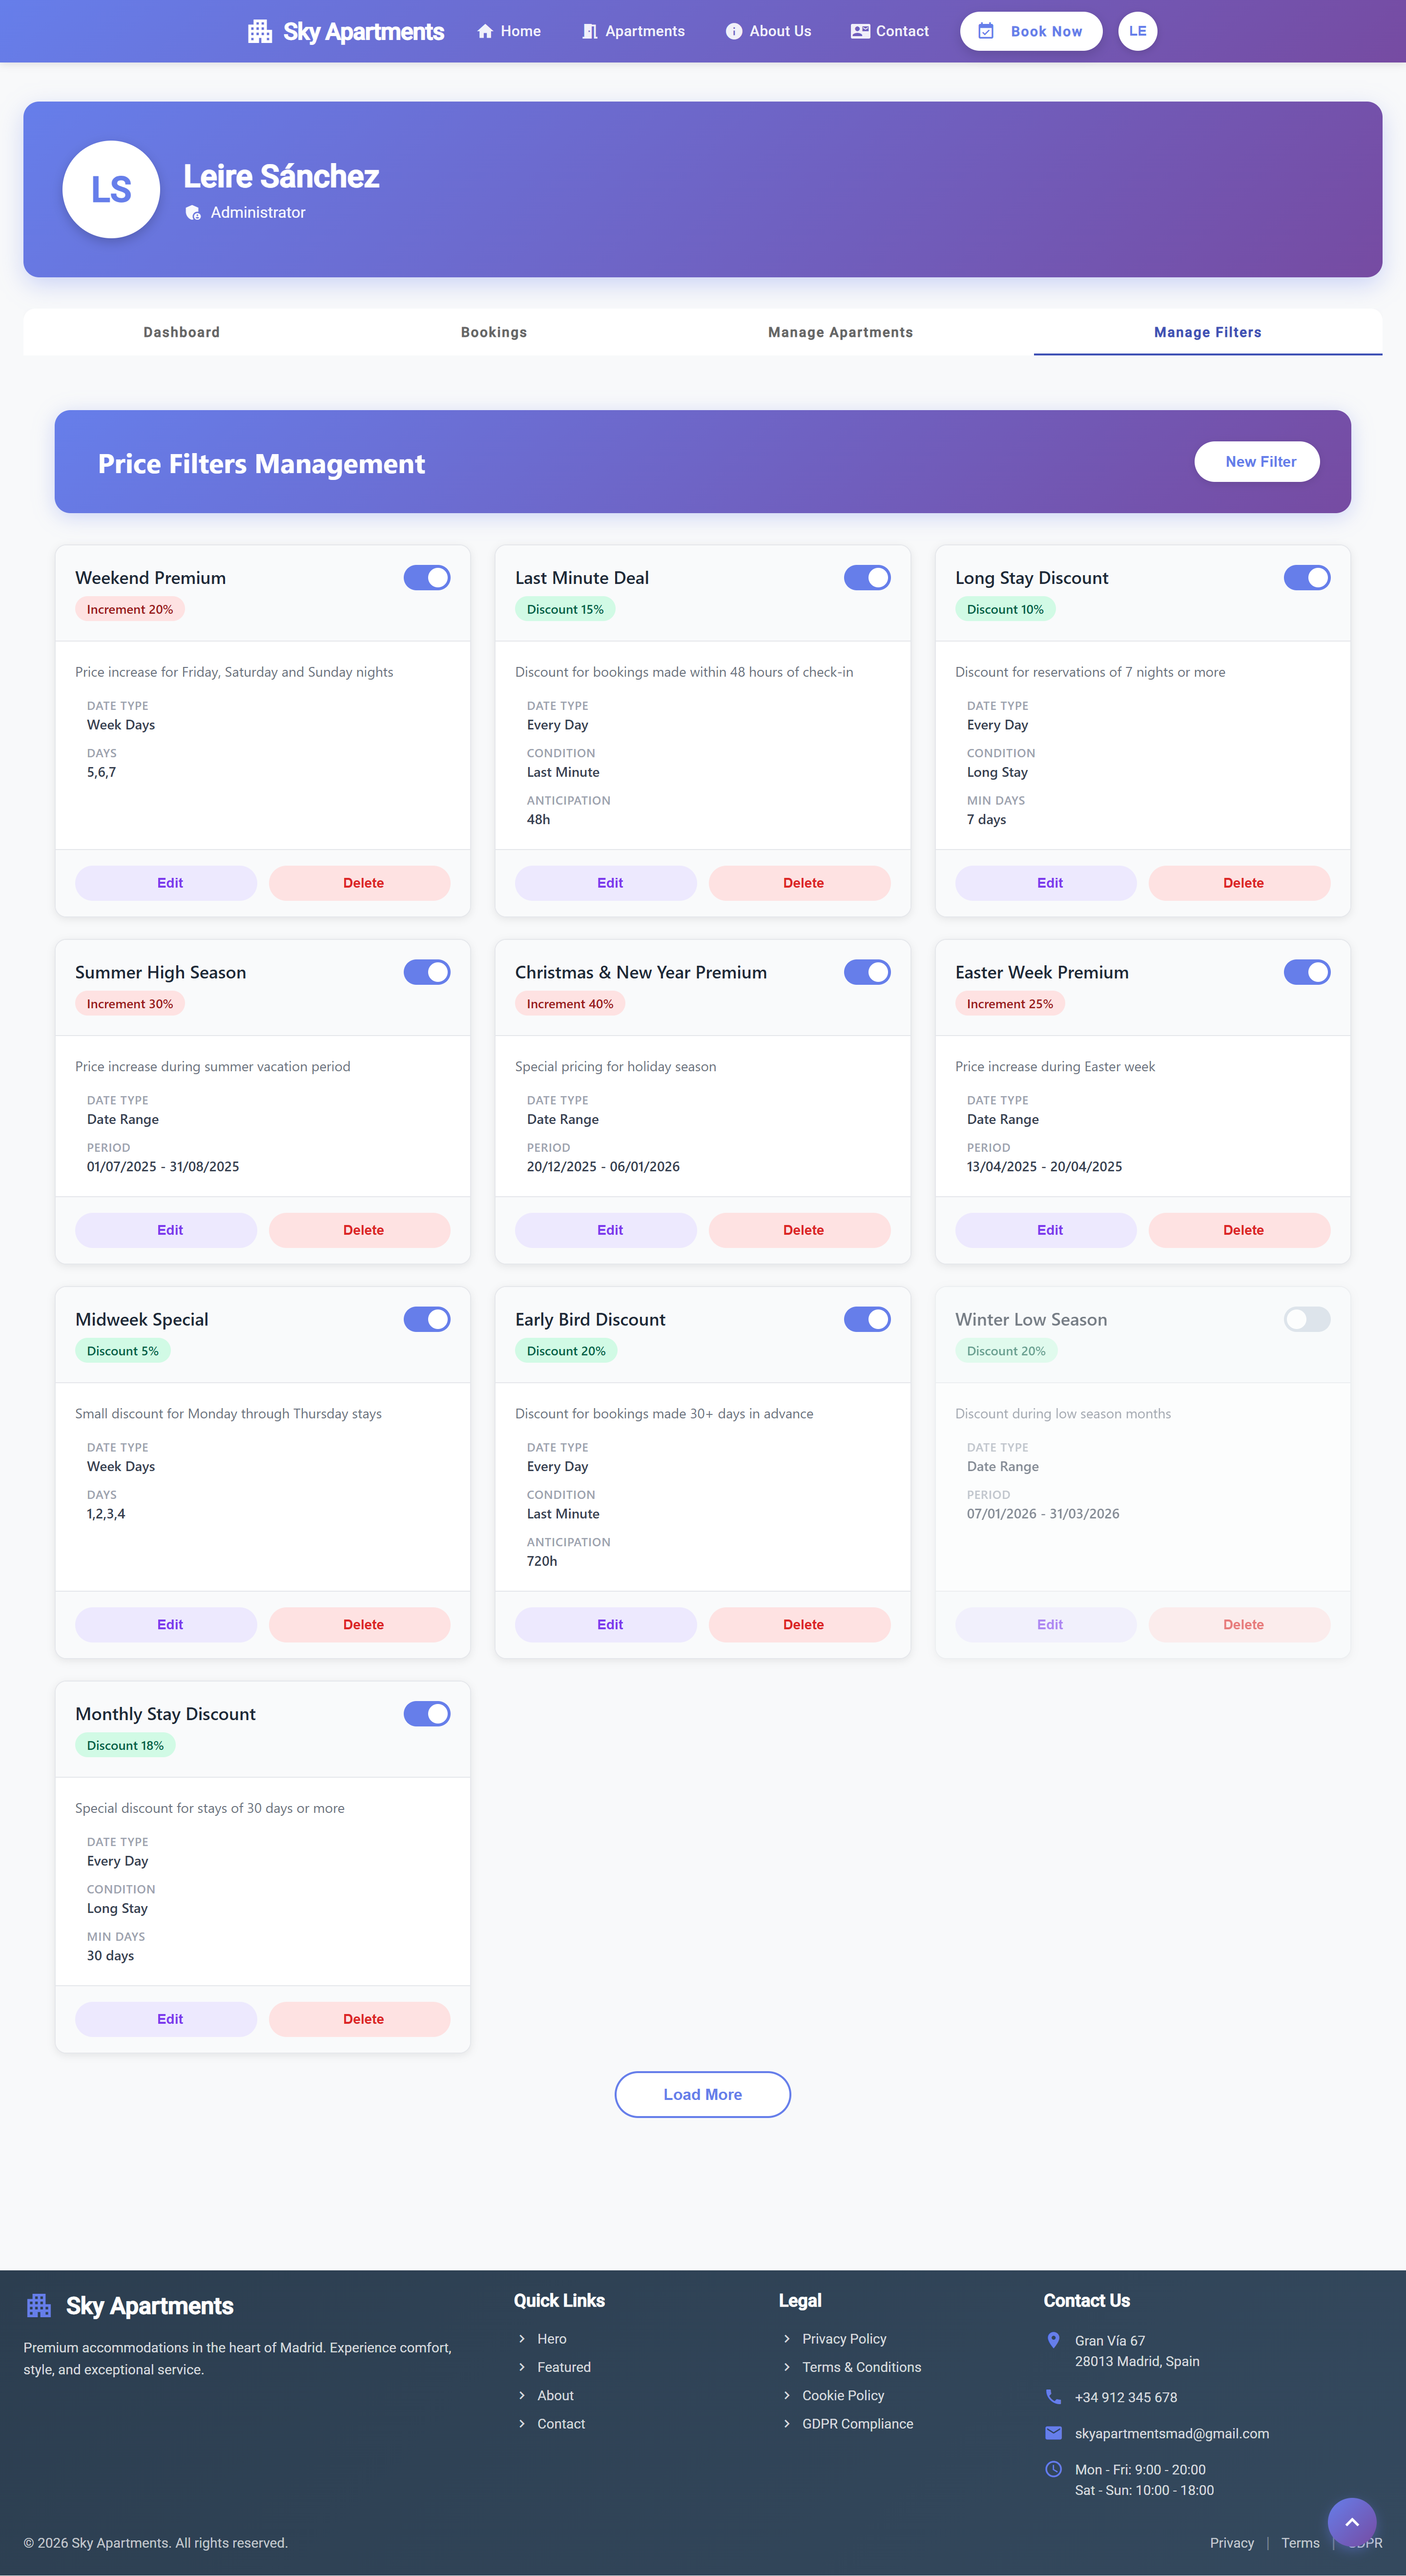
\includegraphics[width=0.8\textwidth]{img/screencapture-13-60-118-214-profile-2026-02-23-21_48_35.png}
    \caption{Listado de reglas y filtros de precios dinámicos configurados en el sistema.}
\end{figure}

Mediante el botón "New Filter", se despliega un modal avanzado que permite crear nuevas reglas. Se pueden configurar incrementos o descuentos porcentuales aplicables a rangos de fechas (temporadas), días de la semana (fines de semana), o condiciones especiales como reservas anticipadas y estancias largas.

\begin{figure}[H]
    \centering
    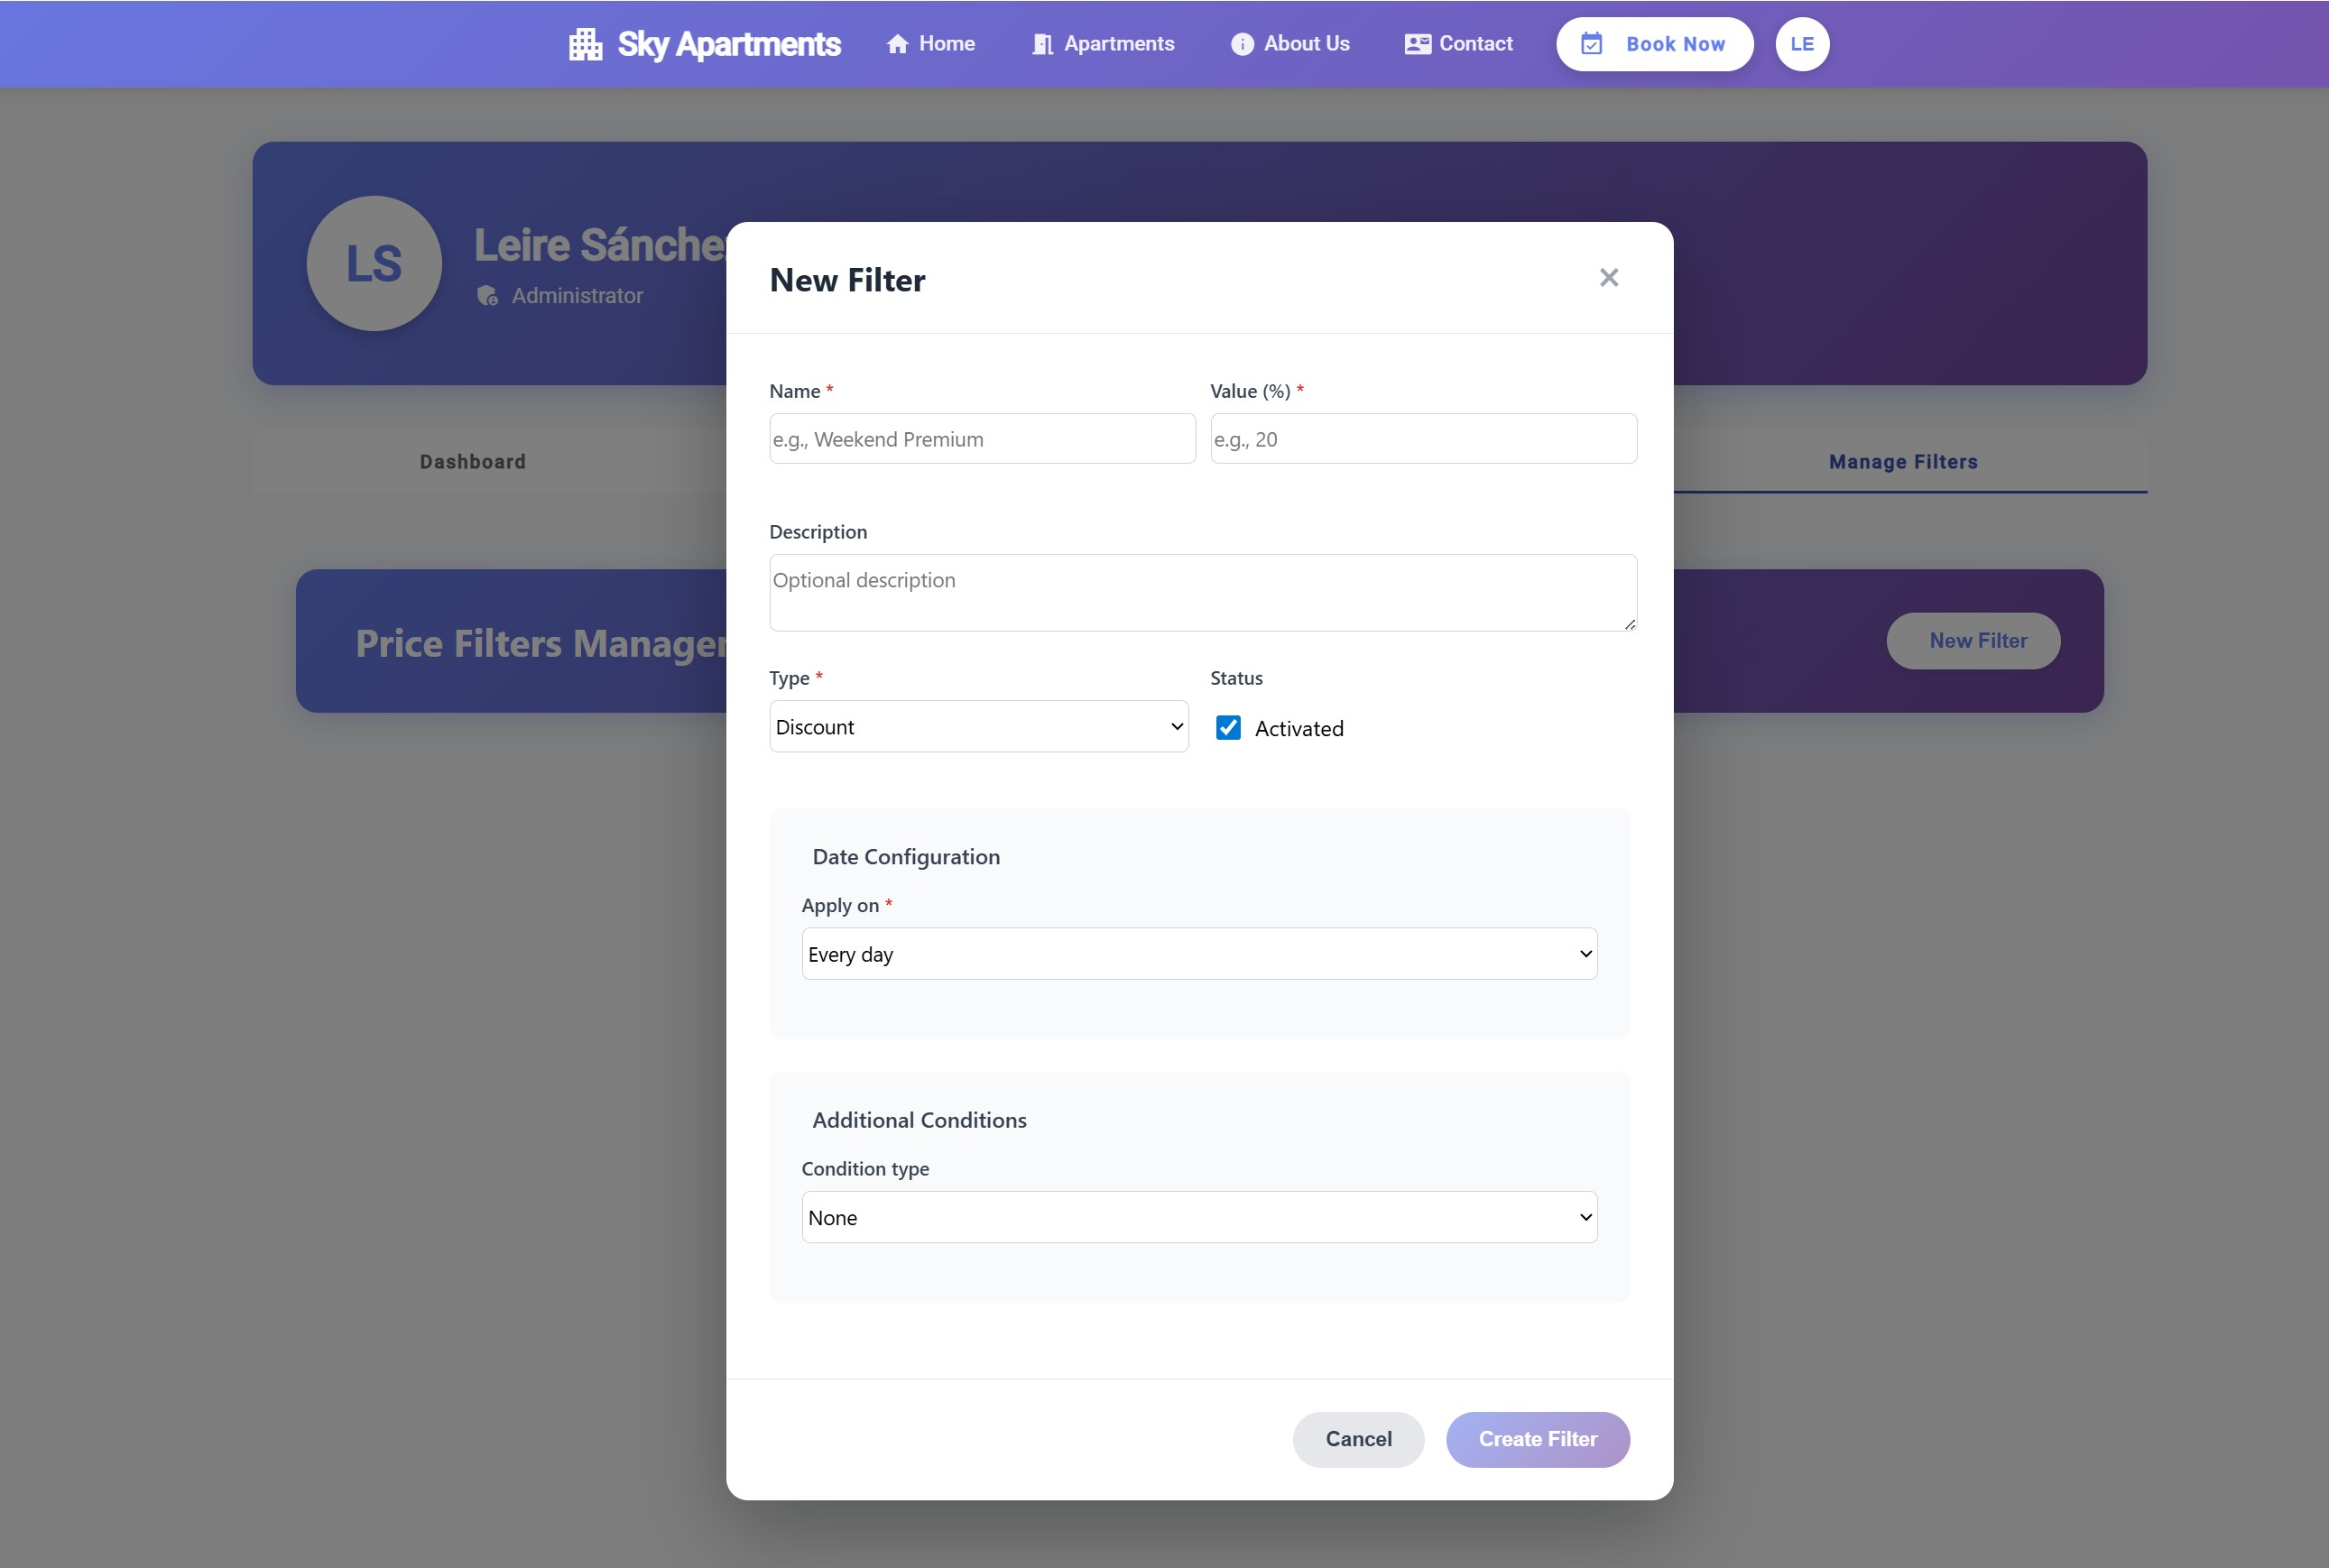
\includegraphics[width=0.8\textwidth]{img/Captura de pantalla 2026-02-23 214959.jpg}
    \caption{Modal de configuración avanzada para una nueva regla de precio dinámico.}
\end{figure}

% Fin del documento
\end{document}
